%********************************************%
%*       Generated from PreTeXt source      *%
%*       on 2020-11-02T16:50:09-06:00       *%
%*   A recent stable commit (2020-08-09):   *%
%* 98f21740783f166a773df4dc83cab5293ab63a4a *%
%*                                          *%
%*         https://pretextbook.org          *%
%*                                          *%
%********************************************%
%% We elect to always write snapshot output into <job>.dep file
\RequirePackage{snapshot}
\documentclass[oneside,10pt,]{book}
%% Custom Preamble Entries, early (use latex.preamble.early)
%% Default LaTeX packages
%%   1.  always employed (or nearly so) for some purpose, or
%%   2.  a stylewriter may assume their presence
\usepackage{geometry}
%% Some aspects of the preamble are conditional,
%% the LaTeX engine is one such determinant
\usepackage{ifthen}
%% etoolbox has a variety of modern conveniences
\usepackage{etoolbox}
\usepackage{ifxetex,ifluatex}
%% Raster graphics inclusion
\usepackage{graphicx}
%% Color support, xcolor package
%% Always loaded, for: add/delete text, author tools
%% Here, since tcolorbox loads tikz, and tikz loads xcolor
\PassOptionsToPackage{usenames,dvipsnames,svgnames,table}{xcolor}
\usepackage{xcolor}
%% begin: defined colors, via xcolor package, for styling
%% end: defined colors, via xcolor package, for styling
%% Colored boxes, and much more, though mostly styling
%% skins library provides "enhanced" skin, employing tikzpicture
%% boxes may be configured as "breakable" or "unbreakable"
%% "raster" controls grids of boxes, aka side-by-side
\usepackage{tcolorbox}
\tcbuselibrary{skins}
\tcbuselibrary{breakable}
\tcbuselibrary{raster}
%% We load some "stock" tcolorbox styles that we use a lot
%% Placement here is provisional, there will be some color work also
%% First, black on white, no border, transparent, but no assumption about titles
\tcbset{ bwminimalstyle/.style={size=minimal, boxrule=-0.3pt, frame empty,
colback=white, colbacktitle=white, coltitle=black, opacityfill=0.0} }
%% Second, bold title, run-in to text/paragraph/heading
%% Space afterwards will be controlled by environment,
%% independent of constructions of the tcb title
%% Places \blocktitlefont onto many block titles
\tcbset{ runintitlestyle/.style={fonttitle=\blocktitlefont\upshape\bfseries, attach title to upper} }
%% Spacing prior to each exercise, anywhere
\tcbset{ exercisespacingstyle/.style={before skip={1.5ex plus 0.5ex}} }
%% Spacing prior to each block
\tcbset{ blockspacingstyle/.style={before skip={2.0ex plus 0.5ex}} }
%% xparse allows the construction of more robust commands,
%% this is a necessity for isolating styling and behavior
%% The tcolorbox library of the same name loads the base library
\tcbuselibrary{xparse}
%% Hyperref should be here, but likes to be loaded late
%%
%% Inline math delimiters, \(, \), need to be robust
%% 2016-01-31:  latexrelease.sty  supersedes  fixltx2e.sty
%% If  latexrelease.sty  exists, bugfix is in kernel
%% If not, bugfix is in  fixltx2e.sty
%% See:  https://tug.org/TUGboat/tb36-3/tb114ltnews22.pdf
%% and read "Fewer fragile commands" in distribution's  latexchanges.pdf
\IfFileExists{latexrelease.sty}{}{\usepackage{fixltx2e}}
%% shorter subnumbers in some side-by-side require manipulations
\usepackage{xstring}
%% Text height identically 9 inches, text width varies on point size
%% See Bringhurst 2.1.1 on measure for recommendations
%% 75 characters per line (count spaces, punctuation) is target
%% which is the upper limit of Bringhurst's recommendations
\geometry{letterpaper,total={340pt,9.0in}}
%% Custom Page Layout Adjustments (use latex.geometry)
%% This LaTeX file may be compiled with pdflatex, xelatex, or lualatex executables
%% LuaTeX is not explicitly supported, but we do accept additions from knowledgeable users
%% The conditional below provides  pdflatex  specific configuration last
%% begin: engine-specific capabilities
\ifthenelse{\boolean{xetex} \or \boolean{luatex}}{%
%% begin: xelatex and lualatex-specific default configuration
\ifxetex\usepackage{xltxtra}\fi
%% realscripts is the only part of xltxtra relevant to lualatex 
\ifluatex\usepackage{realscripts}\fi
%% end:   xelatex and lualatex-specific default configuration
}{
%% begin: pdflatex-specific default configuration
%% We assume a PreTeXt XML source file may have Unicode characters
%% and so we ask LaTeX to parse a UTF-8 encoded file
%% This may work well for accented characters in Western language,
%% but not with Greek, Asian languages, etc.
%% When this is not good enough, switch to the  xelatex  engine
%% where Unicode is better supported (encouraged, even)
\usepackage[utf8]{inputenc}
%% end: pdflatex-specific default configuration
}
%% end:   engine-specific capabilities
%%
%% Fonts.  Conditional on LaTex engine employed.
%% Default Text Font: The Latin Modern fonts are
%% "enhanced versions of the [original TeX] Computer Modern fonts."
%% We use them as the default text font for PreTeXt output.
%% Default Monospace font: Inconsolata (aka zi4)
%% Sponsored by TUG: http://levien.com/type/myfonts/inconsolata.html
%% Loaded for documents with intentional objects requiring monospace
%% See package documentation for excellent instructions
%% fontspec will work universally if we use filename to locate OTF files
%% Loads the "upquote" package as needed, so we don't have to
%% Upright quotes might come from the  textcomp  package, which we also use
%% We employ the shapely \ell to match Google Font version
%% pdflatex: "varl" package option produces shapely \ell
%% pdflatex: "var0" package option produces plain zero (not used)
%% pdflatex: "varqu" package option produces best upright quotes
%% xelatex,lualatex: add OTF StylisticSet 1 for shapely \ell
%% xelatex,lualatex: add OTF StylisticSet 2 for plain zero (not used)
%% xelatex,lualatex: add OTF StylisticSet 3 for upright quotes
%%
%% Automatic Font Control
%% Portions of a document, are, or may, be affected by defined commands
%% These are perhaps more flexible when using  xelatex  rather than  pdflatex
%% The following definitions are meant to be re-defined in a style, using \renewcommand
%% They are scoped when employed (in a TeX group), and so should not be defined with an argument
\newcommand{\divisionfont}{\relax}
\newcommand{\blocktitlefont}{\relax}
\newcommand{\contentsfont}{\relax}
\newcommand{\pagefont}{\relax}
\newcommand{\tabularfont}{\relax}
\newcommand{\xreffont}{\relax}
\newcommand{\titlepagefont}{\relax}
%%
\ifthenelse{\boolean{xetex} \or \boolean{luatex}}{%
%% begin: font setup and configuration for use with xelatex
%% Generally, xelatex is necessary for non-Western fonts
%% fontspec package provides extensive control of system fonts,
%% meaning *.otf (OpenType), and apparently *.ttf (TrueType)
%% that live *outside* your TeX/MF tree, and are controlled by your *system*
%% (it is possible that a TeX distribution will place fonts in a system location)
%%
%% The fontspec package is the best vehicle for using different fonts in  xelatex
%% So we load it always, no matter what a publisher or style might want
%%
\usepackage{fontspec}
%%
%% begin: xelatex main font ("font-xelatex-main" template)
%% Latin Modern Roman is the default font for xelatex and so is loaded with a TU encoding
%% *in the format* so we can't touch it, only perhaps adjust it later
%% in one of two ways (then known by NFSS names such as "lmr")
%% (1) via NFSS with font family names such as "lmr" and "lmss"
%% (2) via fontspec with commands like \setmainfont{Latin Modern Roman}
%% The latter requires the font to be known at the system-level by its font name,
%% but will give access to OTF font features through optional arguments
%% https://tex.stackexchange.com/questions/470008/
%% where-and-how-does-fontspec-sty-specify-the-default-font-latin-modern-roman
%% http://tex.stackexchange.com/questions/115321
%% /how-to-optimize-latin-modern-font-with-xelatex
%%
%% end:   xelatex main font ("font-xelatex-main" template)
%% begin: xelatex mono font ("font-xelatex-mono" template)
%% (conditional on non-trivial uses being present in source)
\IfFontExistsTF{Inconsolatazi4-Regular.otf}{}{\GenericError{}{The font "Inconsolatazi4-Regular.otf" requested by PreTeXt output is not available.  Either a file cannot be located in default locations via a filename, or a font is not known by its name as part of your system.}{Consult the PreTeXt Guide for help with LaTeX fonts.}{}}
\IfFontExistsTF{Inconsolatazi4-Bold.otf}{}{\GenericError{}{The font "Inconsolatazi4-Bold.otf" requested by PreTeXt output is not available.  Either a file cannot be located in default locations via a filename, or a font is not known by its name as part of your system.}{Consult the PreTeXt Guide for help with LaTeX fonts.}{}}
\usepackage{zi4}
\setmonofont[BoldFont=Inconsolatazi4-Bold.otf,StylisticSet={1,3}]{Inconsolatazi4-Regular.otf}
%% end:   xelatex mono font ("font-xelatex-mono" template)
%% begin: xelatex font adjustments ("font-xelatex-style" template)
%% end:   xelatex font adjustments ("font-xelatex-style" template)
%%
%% Extensive support for other languages
\usepackage{polyglossia}
%% Set main/default language based on pretext/@xml:lang value
%% document language code is "en-US", US English
%% usmax variant has extra hypenation
\setmainlanguage[variant=usmax]{english}
%% Enable secondary languages based on discovery of @xml:lang values
%% Enable fonts/scripts based on discovery of @xml:lang values
%% Western languages should be ably covered by Latin Modern Roman
%% end:   font setup and configuration for use with xelatex
}{%
%% begin: font setup and configuration for use with pdflatex
%% begin: pdflatex main font ("font-pdflatex-main" template)
\usepackage{lmodern}
\usepackage[T1]{fontenc}
%% end:   pdflatex main font ("font-pdflatex-main" template)
%% begin: pdflatex mono font ("font-pdflatex-mono" template)
%% (conditional on non-trivial uses being present in source)
\usepackage[varqu,varl]{inconsolata}
%% end:   pdflatex mono font ("font-pdflatex-mono" template)
%% begin: pdflatex font adjustments ("font-pdflatex-style" template)
%% end:   pdflatex font adjustments ("font-pdflatex-style" template)
%% end:   font setup and configuration for use with pdflatex
}
%% Micromanage spacing, etc.  The named "microtype-options"
%% template may be employed to fine-tune package behavior
\usepackage{microtype}
%% Symbols, align environment, commutative diagrams, bracket-matrix
\usepackage{amsmath}
\usepackage{amscd}
\usepackage{amssymb}
%% allow page breaks within display mathematics anywhere
%% level 4 is maximally permissive
%% this is exactly the opposite of AMSmath package philosophy
%% there are per-display, and per-equation options to control this
%% split, aligned, gathered, and alignedat are not affected
\allowdisplaybreaks[4]
%% allow more columns to a matrix
%% can make this even bigger by overriding with  latex.preamble.late  processing option
\setcounter{MaxMatrixCols}{30}
%%
%%
%% Division Titles, and Page Headers/Footers
%% titlesec package, loading "titleps" package cooperatively
%% See code comments about the necessity and purpose of "explicit" option.
%% The "newparttoc" option causes a consistent entry for parts in the ToC 
%% file, but it is only effective if there is a \titleformat for \part.
%% "pagestyles" loads the  titleps  package cooperatively.
\usepackage[explicit, newparttoc, pagestyles]{titlesec}
%% The companion titletoc package for the ToC.
\usepackage{titletoc}
%% Fixes a bug with transition from chapters to appendices in a "book"
%% See generating XSL code for more details about necessity
\newtitlemark{\chaptertitlename}
%% begin: customizations of page styles via the modal "titleps-style" template
%% Designed to use commands from the LaTeX "titleps" package
%% Plain pages should have the same font for page numbers
\renewpagestyle{plain}{%
\setfoot{}{\pagefont\thepage}{}%
}%
%% Single pages as in default LaTeX
\renewpagestyle{headings}{%
\sethead{\pagefont\slshape\MakeUppercase{\ifthechapter{\chaptertitlename\space\thechapter.\space}{}\chaptertitle}}{}{\pagefont\thepage}%
}%
\pagestyle{headings}
%% end: customizations of page styles via the modal "titleps-style" template
%%
%% Create globally-available macros to be provided for style writers
%% These are redefined for each occurence of each division
\newcommand{\divisionnameptx}{\relax}%
\newcommand{\titleptx}{\relax}%
\newcommand{\subtitleptx}{\relax}%
\newcommand{\shortitleptx}{\relax}%
\newcommand{\authorsptx}{\relax}%
\newcommand{\epigraphptx}{\relax}%
%% Create environments for possible occurences of each division
%% Environment for a PTX "preface" at the level of a LaTeX "chapter"
\NewDocumentEnvironment{preface}{mmmmmm}
{%
\renewcommand{\divisionnameptx}{Preface}%
\renewcommand{\titleptx}{#1}%
\renewcommand{\subtitleptx}{#2}%
\renewcommand{\shortitleptx}{#3}%
\renewcommand{\authorsptx}{#4}%
\renewcommand{\epigraphptx}{#5}%
\chapter*{#1}%
\addcontentsline{toc}{chapter}{#3}
\label{#6}%
}{}%
%% Environment for a PTX "chapter" at the level of a LaTeX "chapter"
\NewDocumentEnvironment{chapterptx}{mmmmmm}
{%
\renewcommand{\divisionnameptx}{Chapter}%
\renewcommand{\titleptx}{#1}%
\renewcommand{\subtitleptx}{#2}%
\renewcommand{\shortitleptx}{#3}%
\renewcommand{\authorsptx}{#4}%
\renewcommand{\epigraphptx}{#5}%
\chapter[{#3}]{#1}%
\label{#6}%
}{}%
%% Environment for a PTX "section" at the level of a LaTeX "section"
\NewDocumentEnvironment{sectionptx}{mmmmmm}
{%
\renewcommand{\divisionnameptx}{Section}%
\renewcommand{\titleptx}{#1}%
\renewcommand{\subtitleptx}{#2}%
\renewcommand{\shortitleptx}{#3}%
\renewcommand{\authorsptx}{#4}%
\renewcommand{\epigraphptx}{#5}%
\section[{#3}]{#1}%
\label{#6}%
}{}%
%% Environment for a PTX "subsection" at the level of a LaTeX "subsection"
\NewDocumentEnvironment{subsectionptx}{mmmmmm}
{%
\renewcommand{\divisionnameptx}{Subsection}%
\renewcommand{\titleptx}{#1}%
\renewcommand{\subtitleptx}{#2}%
\renewcommand{\shortitleptx}{#3}%
\renewcommand{\authorsptx}{#4}%
\renewcommand{\epigraphptx}{#5}%
\subsection[{#3}]{#1}%
\label{#6}%
}{}%
%%
%% Styles for six traditional LaTeX divisions
\titleformat{\part}[display]
{\divisionfont\Huge\bfseries\centering}{\divisionnameptx\space\thepart}{30pt}{\Huge#1}
[{\Large\centering\authorsptx}]
\titleformat{\chapter}[display]
{\divisionfont\huge\bfseries}{\divisionnameptx\space\thechapter}{20pt}{\Huge#1}
[{\Large\authorsptx}]
\titleformat{name=\chapter,numberless}[display]
{\divisionfont\huge\bfseries}{}{0pt}{#1}
[{\Large\authorsptx}]
\titlespacing*{\chapter}{0pt}{50pt}{40pt}
\titleformat{\section}[hang]
{\divisionfont\Large\bfseries}{\thesection}{1ex}{#1}
[{\large\authorsptx}]
\titleformat{name=\section,numberless}[block]
{\divisionfont\Large\bfseries}{}{0pt}{#1}
[{\large\authorsptx}]
\titlespacing*{\section}{0pt}{3.5ex plus 1ex minus .2ex}{2.3ex plus .2ex}
\titleformat{\subsection}[hang]
{\divisionfont\large\bfseries}{\thesubsection}{1ex}{#1}
[{\normalsize\authorsptx}]
\titleformat{name=\subsection,numberless}[block]
{\divisionfont\large\bfseries}{}{0pt}{#1}
[{\normalsize\authorsptx}]
\titlespacing*{\subsection}{0pt}{3.25ex plus 1ex minus .2ex}{1.5ex plus .2ex}
\titleformat{\subsubsection}[hang]
{\divisionfont\normalsize\bfseries}{\thesubsubsection}{1em}{#1}
[{\small\authorsptx}]
\titleformat{name=\subsubsection,numberless}[block]
{\divisionfont\normalsize\bfseries}{}{0pt}{#1}
[{\normalsize\authorsptx}]
\titlespacing*{\subsubsection}{0pt}{3.25ex plus 1ex minus .2ex}{1.5ex plus .2ex}
\titleformat{\paragraph}[hang]
{\divisionfont\normalsize\bfseries}{\theparagraph}{1em}{#1}
[{\small\authorsptx}]
\titleformat{name=\paragraph,numberless}[block]
{\divisionfont\normalsize\bfseries}{}{0pt}{#1}
[{\normalsize\authorsptx}]
\titlespacing*{\paragraph}{0pt}{3.25ex plus 1ex minus .2ex}{1.5em}
%%
%% Styles for five traditional LaTeX divisions
\titlecontents{part}%
[0pt]{\contentsmargin{0em}\addvspace{1pc}\contentsfont\bfseries}%
{\Large\thecontentslabel\enspace}{\Large}%
{}%
[\addvspace{.5pc}]%
\titlecontents{chapter}%
[0pt]{\contentsmargin{0em}\addvspace{1pc}\contentsfont\bfseries}%
{\large\thecontentslabel\enspace}{\large}%
{\hfill\bfseries\thecontentspage}%
[\addvspace{.5pc}]%
\dottedcontents{section}[3.8em]{\contentsfont}{2.3em}{1pc}%
\dottedcontents{subsection}[6.1em]{\contentsfont}{3.2em}{1pc}%
\dottedcontents{subsubsection}[9.3em]{\contentsfont}{4.3em}{1pc}%
%%
%% Begin: Semantic Macros
%% To preserve meaning in a LaTeX file
%%
%% \mono macro for content of "c", "cd", "tag", etc elements
%% Also used automatically in other constructions
%% Simply an alias for \texttt
%% Always defined, even if there is no need, or if a specific tt font is not loaded
\newcommand{\mono}[1]{\texttt{#1}}
%%
%% Following semantic macros are only defined here if their
%% use is required only in this specific document
%%
%% Used for warnings, typically bold and italic
\newcommand{\alert}[1]{\textbf{\textit{#1}}}
%% Used for fillin answer blank
%% Argument is length in em
%% Length may compress for output to fit in one line
\newcommand{\fillin}[1]{\leavevmode\leaders\vrule height -1.2pt depth 1.5pt \hskip #1em minus #1em \null}
%% End: Semantic Macros
%% Division Numbering: Chapters, Sections, Subsections, etc
%% Division numbers may be turned off at some level ("depth")
%% A section *always* has depth 1, contrary to us counting from the document root
%% The latex default is 3.  If a larger number is present here, then
%% removing this command may make some cross-references ambiguous
%% The precursor variable $numbering-maxlevel is checked for consistency in the common XSL file
\setcounter{secnumdepth}{3}
%%
%% AMS "proof" environment is no longer used, but we leave previously
%% implemented \qedhere in place, should the LaTeX be recycled
\newcommand{\qedhere}{\relax}
%%
%% A faux tcolorbox whose only purpose is to provide common numbering
%% facilities for most blocks (possibly not projects, 2D displays)
%% Controlled by  numbering.theorems.level  processing parameter
\newtcolorbox[auto counter, number within=section]{block}{}
%%
%% This document is set to number PROJECT-LIKE on a separate numbering scheme
%% So, a faux tcolorbox whose only purpose is to provide this numbering
%% Controlled by  numbering.projects.level  processing parameter
\newtcolorbox[auto counter, number within=section]{project-distinct}{}
%% A faux tcolorbox whose only purpose is to provide common numbering
%% facilities for 2D displays which are subnumbered as part of a "sidebyside"
\makeatletter
\newtcolorbox[auto counter, number within=tcb@cnt@block, number freestyle={\noexpand\thetcb@cnt@block(\noexpand\alph{\tcbcounter})}]{subdisplay}{}
\makeatother
%%
%% tcolorbox, with styles, for THEOREM-LIKE
%%
%% theorem: fairly simple numbered block/structure
\tcbset{ theoremstyle/.style={bwminimalstyle, runintitlestyle, blockspacingstyle, after title={\space}, } }
\newtcolorbox[use counter from=block]{theorem}[3]{title={{Theorem~\thetcbcounter\notblank{#1#2}{\space}{}\notblank{#1}{\space#1}{}\notblank{#2}{\space(#2)}{}}}, phantomlabel={#3}, breakable, parbox=false, after={\par}, fontupper=\itshape, theoremstyle, }
%% corollary: fairly simple numbered block/structure
\tcbset{ corollarystyle/.style={bwminimalstyle, runintitlestyle, blockspacingstyle, after title={\space}, } }
\newtcolorbox[use counter from=block]{corollary}[3]{title={{Corollary~\thetcbcounter\notblank{#1#2}{\space}{}\notblank{#1}{\space#1}{}\notblank{#2}{\space(#2)}{}}}, phantomlabel={#3}, breakable, parbox=false, after={\par}, fontupper=\itshape, corollarystyle, }
%%
%% tcolorbox, with styles, for DEFINITION-LIKE
%%
%% definition: fairly simple numbered block/structure
\tcbset{ definitionstyle/.style={bwminimalstyle, runintitlestyle, blockspacingstyle, after title={\space}, after upper={\space\space\hspace*{\stretch{1}}\(\lozenge\)}, } }
\newtcolorbox[use counter from=block]{definition}[2]{title={{Definition~\thetcbcounter\notblank{#1}{\space\space#1}{}}}, phantomlabel={#2}, breakable, parbox=false, after={\par}, definitionstyle, }
%%
%% tcolorbox, with styles, for EXAMPLE-LIKE
%%
%% example: fairly simple numbered block/structure
\tcbset{ examplestyle/.style={bwminimalstyle, runintitlestyle, blockspacingstyle, after title={\space}, after upper={\space\space\hspace*{\stretch{1}}\(\square\)}, } }
\newtcolorbox[use counter from=block]{example}[2]{title={{Example~\thetcbcounter\notblank{#1}{\space\space#1}{}}}, phantomlabel={#2}, breakable, parbox=false, after={\par}, examplestyle, }
%%
%% tcolorbox, with styles, for inline exercises
%%
%% inlineexercise: fairly simple numbered block/structure
\tcbset{ inlineexercisestyle/.style={bwminimalstyle, runintitlestyle, blockspacingstyle, after title={\space}, } }
\newtcolorbox[use counter from=block]{inlineexercise}[2]{title={{Checkpoint~\thetcbcounter\notblank{#1}{\space\space#1}{}}}, phantomlabel={#2}, breakable, parbox=false, after={\par}, inlineexercisestyle, }
%%
%% tcolorbox, with styles, for FIGURE-LIKE
%%
%% tableptx: 2-D display structure
\tcbset{ tableptxstyle/.style={bwminimalstyle, middle=1ex, blockspacingstyle, coltitle=black, bottomtitle=2ex, titlerule=-0.3pt, fonttitle=\blocktitlefont} }
\newtcolorbox[use counter from=block]{tableptx}[3]{title={{\textbf{Table~\thetcbcounter}\space#1}}, phantomlabel={#2}, unbreakable, parbox=false, tableptxstyle, }
%%
%% xparse environments for introductions and conclusions of divisions
%%
%% introduction: in a structured division
\NewDocumentEnvironment{introduction}{m}
{\notblank{#1}{\noindent\textbf{#1}\space}{}}{\par\medskip}
%%
%% tcolorbox, with styles, for miscellaneous environments
%%
%% proof: title is a replacement
\tcbset{ proofstyle/.style={bwminimalstyle, fonttitle=\blocktitlefont\itshape, attach title to upper, after title={\space}, after upper={\space\space\hspace*{\stretch{1}}\(\blacksquare\)},
} }
\newtcolorbox{proof}[2]{title={\notblank{#1}{#1}{Proof.}}, phantom={\hypertarget{#2}{}}, breakable, parbox=false, after={\par}, proofstyle }
%% Localize LaTeX supplied names (possibly none)
\renewcommand*{\chaptername}{Chapter}
%% Equation Numbering
%% Controlled by  numbering.equations.level  processing parameter
%% No adjustment here implies document-wide numbering
\numberwithin{equation}{section}
%% "tcolorbox" environment for a single image, occupying entire \linewidth
%% arguments are left-margin, width, right-margin, as multiples of
%% \linewidth, and are guaranteed to be positive and sum to 1.0
\tcbset{ imagestyle/.style={bwminimalstyle} }
\NewTColorBox{image}{mmm}{imagestyle,left skip=#1\linewidth,width=#2\linewidth}
%% For improved tables
\usepackage{array}
%% Some extra height on each row is desirable, especially with horizontal rules
%% Increment determined experimentally
\setlength{\extrarowheight}{0.2ex}
%% Define variable thickness horizontal rules, full and partial
%% Thicknesses are 0.03, 0.05, 0.08 in the  booktabs  package
\newcommand{\hrulethin}  {\noalign{\hrule height 0.04em}}
\newcommand{\hrulemedium}{\noalign{\hrule height 0.07em}}
\newcommand{\hrulethick} {\noalign{\hrule height 0.11em}}
%% We preserve a copy of the \setlength package before other
%% packages (extpfeil) get a chance to load packages that redefine it
\let\oldsetlength\setlength
\newlength{\Oldarrayrulewidth}
\newcommand{\crulethin}[1]%
{\noalign{\global\oldsetlength{\Oldarrayrulewidth}{\arrayrulewidth}}%
\noalign{\global\oldsetlength{\arrayrulewidth}{0.04em}}\cline{#1}%
\noalign{\global\oldsetlength{\arrayrulewidth}{\Oldarrayrulewidth}}}%
\newcommand{\crulemedium}[1]%
{\noalign{\global\oldsetlength{\Oldarrayrulewidth}{\arrayrulewidth}}%
\noalign{\global\oldsetlength{\arrayrulewidth}{0.07em}}\cline{#1}%
\noalign{\global\oldsetlength{\arrayrulewidth}{\Oldarrayrulewidth}}}
\newcommand{\crulethick}[1]%
{\noalign{\global\oldsetlength{\Oldarrayrulewidth}{\arrayrulewidth}}%
\noalign{\global\oldsetlength{\arrayrulewidth}{0.11em}}\cline{#1}%
\noalign{\global\oldsetlength{\arrayrulewidth}{\Oldarrayrulewidth}}}
%% Single letter column specifiers defined via array package
\newcolumntype{A}{!{\vrule width 0.04em}}
\newcolumntype{B}{!{\vrule width 0.07em}}
\newcolumntype{C}{!{\vrule width 0.11em}}
%% Program listing support: for listings, programs, consoles, and Sage code
\ifthenelse{\boolean{xetex} \or \boolean{luatex}}%
  {\tcbuselibrary{listings}}%
  {\tcbuselibrary{listingsutf8}}%
%% We define the listings font style to be the default "ttfamily"
%% To fix hyphens/dashes rendered in PDF as fancy minus signs by listing
%% http://tex.stackexchange.com/questions/33185/listings-package-changes-hyphens-to-minus-signs
\makeatletter
\lst@CCPutMacro\lst@ProcessOther {"2D}{\lst@ttfamily{-{}}{-{}}}
\@empty\z@\@empty
\makeatother
%% We define a null language, free of any formatting or style
%% for use when a language is not supported, or pseudo-code, or consoles
%% Not necessary for Sage code, so in limited cases included unnecessarily
\lstdefinelanguage{none}{identifierstyle=,commentstyle=,stringstyle=,keywordstyle=}
\ifthenelse{\boolean{xetex}}{}{%
%% begin: pdflatex-specific listings configuration
%% translate U+0080 - U+00F0 to their textmode LaTeX equivalents
%% Data originally from https://www.w3.org/Math/characters/unicode.xml, 2016-07-23
%% Lines marked in XSL with "$" were converted from mathmode to textmode
\lstset{extendedchars=true}
\lstset{literate={ }{{~}}{1}{¡}{{\textexclamdown }}{1}{¢}{{\textcent }}{1}{£}{{\textsterling }}{1}{¤}{{\textcurrency }}{1}{¥}{{\textyen }}{1}{¦}{{\textbrokenbar }}{1}{§}{{\textsection }}{1}{¨}{{\textasciidieresis }}{1}{©}{{\textcopyright }}{1}{ª}{{\textordfeminine }}{1}{«}{{\guillemotleft }}{1}{¬}{{\textlnot }}{1}{­}{{\-}}{1}{®}{{\textregistered }}{1}{¯}{{\textasciimacron }}{1}{°}{{\textdegree }}{1}{±}{{\textpm }}{1}{²}{{\texttwosuperior }}{1}{³}{{\textthreesuperior }}{1}{´}{{\textasciiacute }}{1}{µ}{{\textmu }}{1}{¶}{{\textparagraph }}{1}{·}{{\textperiodcentered }}{1}{¸}{{\c{}}}{1}{¹}{{\textonesuperior }}{1}{º}{{\textordmasculine }}{1}{»}{{\guillemotright }}{1}{¼}{{\textonequarter }}{1}{½}{{\textonehalf }}{1}{¾}{{\textthreequarters }}{1}{¿}{{\textquestiondown }}{1}{À}{{\`{A}}}{1}{Á}{{\'{A}}}{1}{Â}{{\^{A}}}{1}{Ã}{{\~{A}}}{1}{Ä}{{\"{A}}}{1}{Å}{{\AA }}{1}{Æ}{{\AE }}{1}{Ç}{{\c{C}}}{1}{È}{{\`{E}}}{1}{É}{{\'{E}}}{1}{Ê}{{\^{E}}}{1}{Ë}{{\"{E}}}{1}{Ì}{{\`{I}}}{1}{Í}{{\'{I}}}{1}{Î}{{\^{I}}}{1}{Ï}{{\"{I}}}{1}{Ð}{{\DH }}{1}{Ñ}{{\~{N}}}{1}{Ò}{{\`{O}}}{1}{Ó}{{\'{O}}}{1}{Ô}{{\^{O}}}{1}{Õ}{{\~{O}}}{1}{Ö}{{\"{O}}}{1}{×}{{\texttimes }}{1}{Ø}{{\O }}{1}{Ù}{{\`{U}}}{1}{Ú}{{\'{U}}}{1}{Û}{{\^{U}}}{1}{Ü}{{\"{U}}}{1}{Ý}{{\'{Y}}}{1}{Þ}{{\TH }}{1}{ß}{{\ss }}{1}{à}{{\`{a}}}{1}{á}{{\'{a}}}{1}{â}{{\^{a}}}{1}{ã}{{\~{a}}}{1}{ä}{{\"{a}}}{1}{å}{{\aa }}{1}{æ}{{\ae }}{1}{ç}{{\c{c}}}{1}{è}{{\`{e}}}{1}{é}{{\'{e}}}{1}{ê}{{\^{e}}}{1}{ë}{{\"{e}}}{1}{ì}{{\`{\i}}}{1}{í}{{\'{\i}}}{1}{î}{{\^{\i}}}{1}{ï}{{\"{\i}}}{1}{ð}{{\dh }}{1}{ñ}{{\~{n}}}{1}{ò}{{\`{o}}}{1}{ó}{{\'{o}}}{1}{ô}{{\^{o}}}{1}{õ}{{\~{o}}}{1}{ö}{{\"{o}}}{1}{÷}{{\textdiv }}{1}{ø}{{\o }}{1}{ù}{{\`{u}}}{1}{ú}{{\'{u}}}{1}{û}{{\^{u}}}{1}{ü}{{\"{u}}}{1}{ý}{{\'{y}}}{1}{þ}{{\th }}{1}{ÿ}{{\"{y}}}{1}}
%% end: pdflatex-specific listings configuration
}
%% End of generic listing adjustments
%% The listings package as tcolorbox for Sage code
%% We do as much styling as possible with tcolorbox, not listings
%% Sage's blue is 50%, we go way lighter (blue!05 would also work)
%% Note that we defuse listings' default "aboveskip" and "belowskip"
\definecolor{sageblue}{rgb}{0.95,0.95,1}
\tcbset{ sagestyle/.style={left=0pt, right=0pt, top=0ex, bottom=0ex, middle=0pt, toptitle=0pt, bottomtitle=0pt,
boxsep=4pt, listing only, fontupper=\small\ttfamily,
breakable, parbox=false, 
listing options={language=Python,breaklines=true,breakatwhitespace=true, extendedchars=true, aboveskip=0pt, belowskip=0pt}} }
\newtcblisting{sageinput}{sagestyle, colback=sageblue, sharp corners, boxrule=0.5pt, toprule at break=-0.3pt, bottomrule at break=-0.3pt, }
\newtcblisting{sageoutput}{sagestyle, colback=white, colframe=white, frame empty, before skip=0pt, after skip=0pt, }
%% Fancy Verbatim for consoles, preformatted, code display, literate programming
\usepackage{fancyvrb}
%% Pre-formatted text, a peer of paragraphs
\DefineVerbatimEnvironment{preformatted}{Verbatim}{}
%% More flexible list management, esp. for references
%% But also for specifying labels (i.e. custom order) on nested lists
\usepackage[inline]{enumitem}
%% hyperref driver does not need to be specified, it will be detected
%% Footnote marks in tcolorbox have broken linking under
%% hyperref, so it is necessary to turn off all linking
%% It *must* be given as a package option, not with \hypersetup
\usepackage[hyperfootnotes=false]{hyperref}
%% configure hyperref's  \url  to match listings' inline verbatim
\renewcommand\UrlFont{\small\ttfamily}
%% Hyperlinking active in electronic PDFs, all links solid and blue
\hypersetup{colorlinks=true,linkcolor=blue,citecolor=blue,filecolor=blue,urlcolor=blue}
\hypersetup{pdftitle={Essentials of Mathematical Probability and Statistics}}
%% If you manually remove hyperref, leave in this next command
\providecommand\phantomsection{}
%% Graphics Preamble Entries
\usepackage{tikz}
\usetikzlibrary{backgrounds}
\usetikzlibrary{arrows,matrix}
\usetikzlibrary{snakes}
%% If tikz has been loaded, replace ampersand with \amp macro
%% tcolorbox styles for sidebyside layout
\tcbset{ sbsstyle/.style={raster before skip=2.0ex, raster equal height=rows, raster force size=false} }
\tcbset{ sbspanelstyle/.style={bwminimalstyle, fonttitle=\blocktitlefont} }
%% Enviroments for side-by-side and components
%% Necessary to use \NewTColorBox for boxes of the panels
%% "newfloat" environment to squash page-breaks within a single sidebyside
%% "xparse" environment for entire sidebyside
\NewDocumentEnvironment{sidebyside}{mmmm}
  {\begin{tcbraster}
    [sbsstyle,raster columns=#1,
    raster left skip=#2\linewidth,raster right skip=#3\linewidth,raster column skip=#4\linewidth]}
  {\end{tcbraster}}
%% "tcolorbox" environment for a panel of sidebyside
\NewTColorBox{sbspanel}{mO{top}}{sbspanelstyle,width=#1\linewidth,valign=#2}
%% extpfeil package for certain extensible arrows,
%% as also provided by MathJax extension of the same name
%% NB: this package loads mtools, which loads calc, which redefines
%%     \setlength, so it can be removed if it seems to be in the 
%%     way and your math does not use:
%%     
%%     \xtwoheadrightarrow, \xtwoheadleftarrow, \xmapsto, \xlongequal, \xtofrom
%%     
%%     we have had to be extra careful with variable thickness
%%     lines in tables, and so also load this package late
\usepackage{extpfeil}
%% Custom Preamble Entries, late (use latex.preamble.late)
%% Begin: Author-provided packages
%% (From  docinfo/latex-preamble/package  elements)
%% End: Author-provided packages
%% Begin: Author-provided macros
%% (From  docinfo/macros  element)
%% Plus three from MBX for XML characters

\newcommand{\lt}{<}
\newcommand{\gt}{>}
\newcommand{\amp}{&}
%% End: Author-provided macros
\begin{document}
\frontmatter
%% begin: half-title
\thispagestyle{empty}
{\titlepagefont\centering
\vspace*{0.28\textheight}
{\Huge Essentials of Mathematical Probability and Statistics}\\}
\clearpage
%% end:   half-title
%% begin: title page
%% Inspired by Peter Wilson's "titleDB" in "titlepages" CTAN package
\thispagestyle{empty}
{\titlepagefont\centering
\vspace*{0.14\textheight}
%% Target for xref to top-level element is ToC
\addtocontents{toc}{\protect\hypertarget{x:book:Essentials_Probability_And_Statistics}{}}
{\Huge Essentials of Mathematical Probability and Statistics}\\[3\baselineskip]
{\Large John Travis}\\[0.5\baselineskip]
{\Large Mississippi College}\\[3\baselineskip]
{\Large }\\[0.5\baselineskip]
[3\baselineskip]
{\Large November 2, 2020}\\}
\clearpage
%% end:   title page
%% begin: copyright-page
\thispagestyle{empty}
\hypertarget{g:colophon:idp1}{}\noindent
John Travis grew up in Mississippi and did his graduate work at the University of Tennessee and Mississippi State University. As a numerical analyst, since 1988 he has been a professor of mathematics at his undergraduate alma mater Mississippi College where he currently serves as Professor of Mathematics.%
\par
John is married to Ruth Page Travis and together they have three unique daughters.  All are good at mathematics.%
\par
You can find him playing racquetball or guitar but not generally at the same time. He is also an active supporter and organizer for the opensouce online homework system WeBWorK.%
\par
\vspace*{\stretch{2}}
\noindent\textcopyright{}2015 \textendash{}today\quad{}John Travis\\[0.5\baselineskip]
Permission is granted to copy, distribute and\slash{}or modify this document under the terms of the GNU Free Documentation License, Version 1.2 or any later version published by the Free Software Foundation; with no Invariant Sections, no Front-Cover Texts, and no Back-Cover Texts.  A copy of the license is included in the appendix entitled ``GNU Free Documentation License.''\par\medskip
\vspace*{\stretch{1}}
\null\clearpage
%% end:   copyright-page
%
%
\typeout{************************************************}
\typeout{Preface  Preface}
\typeout{************************************************}
%
\begin{preface}{Preface}{}{Preface}{}{}{g:preface:idp2}
This text is intended for a one-semester course in probability and statistics that presumes calculus knowledge up to integration techniques. It is perhaps helpful if a student has already been exposed to sequences and series but much of what is needed is reviewed in the text.%
\par
An interactive version of this text is available at%
\par
\href{http://math.mc.edu/travis/mathbook/Probability/Essentials_Probability_And_Statistics.html}{http:\slash{}\slash{}math.mc.edu\slash{}travis\slash{}mathbook\slash{}Probability\slash{}Essentials\textunderscore{}Probability\textunderscore{}And\textunderscore{}Statistics.html} http:\slash{}\slash{}math.mc.edu\slash{}travis\slash{}mathbook\slash{}Probability\slash{}Essentials\textunderscore{}Probability\textunderscore{}And\textunderscore{}Statistics.html%
\par
and an pdf version with active links is available at%
\par
\href{http://math.mc.edu/travis/mathbook/Probability/Essentials_Probability_And_Statistics.pdf}{http:\slash{}\slash{}math.mc.edu\slash{}travis\slash{}mathbook\slash{}Probability\slash{}Essentials\textunderscore{}Probability\textunderscore{}And\textunderscore{}Statistics.pdf} http:\slash{}\slash{}math.mc.edu\slash{}travis\slash{}mathbook\slash{}Probability\slash{}Essentials\textunderscore{}Probability\textunderscore{}And\textunderscore{}Statistics.pdf .%
\par
A collection of WeBWorK online homework problems are available to correlate with the material in this text. Copies of these sets of problems are available by contacting the author. These exercises are considered an integral part when using this text although a static version of these is included in the appendix.%
\par
To successfully utilize this text, a student should review the requisite material and perhaps review the proofs and derivations if appropriate. While moving through the text, the student should review each of the examples and then attempt each of the interactive WeBWorK exercises. Whenever an interactive cell comes up, the student should play around with the cell and perhaps change the input data as appropriate to experiment. When a section is completed, a student should work the WeBWorK exercises (not part of this text) or some other exercises provided by the instructor and attempt the exercises provided in this text...many of which are famous examples or exercises that might have special significance.  Some are (of course) just easy and most of the textbook exercises have solutions provided.%
\par
WeBWorK (\href{http://webwork.maa.org}{webwork.maa.org}) is an open-source online homework system for math and science courses. WeBWorK is supported by the MAA and the NSF and comes with a Open Problem Library (OPL) of over 35,000 homework problems. Problems in the OPL target most lower division undergraduate math courses and some advanced courses. Supported courses include college algebra, discrete mathematics, probability and statistics, single and multivariable calculus, differential equations, linear algebra and complex analysis.%
\par
Sage (\href{http://sagemath.org}{sagemath.org}) is a free, open-source, software system for advanced mathematics, which is ideal for assisting with a study of abstract algebra. Sage can be used either on your own computer, a local server, or on SageMathCloud (\href{https://cloud.sagemath.com}{https:\slash{}\slash{}cloud.sagemath.com}).%
\par
R (\href{https://www.r-project.org/}{https:\slash{}\slash{}www.r-project.org\slash{}}) is a programming language and free software environment for statistical computing and graphics supported by the R Foundation for Statistical Computing. The R language is widely used among statisticians and data miners for developing statistical software and data analysis. In this text, the sage cell is used also for interactive computations related to R.%
\nopagebreak\par%
\hfill\begin{tabular}[t]{l@{}}
John Travis\\
Clinton, Mississippi 2015-2019
\end{tabular}\\\par
\end{preface}
%% begin: table of contents
%% Adjust Table of Contents
\setcounter{tocdepth}{1}
\renewcommand*\contentsname{Contents}
\tableofcontents
%% end:   table of contents
\mainmatter
%
%
\typeout{************************************************}
\typeout{Chapter 1 Statistical Measures}
\typeout{************************************************}
%
\begin{chapterptx}{Statistical Measures}{}{Statistical Measures}{}{}{x:chapter:RepresentingData}
%
%
\typeout{************************************************}
\typeout{Section 1.1 Making Inferences}
\typeout{************************************************}
%
\begin{sectionptx}{Making Inferences}{}{Making Inferences}{}{}{x:section:DataIntroduction}
To compute your final grade in a class your teacher will likely consider the scores you have earned on various assignments and examinations completed during the duration of the course. However, she ultimately will likely be required to assign some numerical score indicating your level of success in the course. One grade to rule them all. This final grade can only be one value and it would make sense that the grade be a reflection of your work on these tasks. So, what is a fair way for your teacher to complete this task?%
\par
Through this process, you will also often need to take into account whether that data set is the entire list of possibilities-{}-{}known as the population-{}-{}or just a subset of that population perhaps obtained by taking repeated measurements -{}-{}that is, a sample.%
\par
In general, it is often useful to make decisions using quantitative data but making those decisions can be somewhat arbitrary without a mathematical basis supporting those decisions. In this chapter, you will consider a number of ways to use point values to represent a given set of data. Each of these quantitative metrics will be called a "statistical measure" and will, in some fashion, describe using one number some property of the entire data set. Such measures are part of what is known as "descriptive statistics".  Later, you will learn about how other metrics can be used to predict properties of the underlying situation. Doing this is part of what is known as "inferential statistics".%
\par
So, let's go and hopefully you will in some measure enjoy the ride!%
\end{sectionptx}
%
%
\typeout{************************************************}
\typeout{Section 1.2 Measurement Scales}
\typeout{************************************************}
%
\begin{sectionptx}{Measurement Scales}{}{Measurement Scales}{}{}{x:section:MeasurementScales}
In creating statistical measures, you might want to consider one of the following general types.%
\par
%
\begin{itemize}[label=\textbullet]
\item{}Nominal measures - In this case, data falls into mutually exclusive and exhaustive categories for which the numerical value is only used for identification purposes. For example, assigning Male = 1, Female = -1.%
\item{}Ordinal measures - In this case, data consists of discrete numerical values which can be ranked from lowest to highest or vice versa. For example, your grades in a number of classes are used to compute your GPA-{}-{}which is a single number.%
\item{}Interval measures - In this case, data possesses an order and where the distance between data values is of significance. For example, heights and weights.%
\item{}Ratio measures - In this case, data can be expressed as a position in some interval and where ratios between observations have meaning. For example, percentile rankings%
\end{itemize}
%
\par
In the subsequent sections of this chapter, you will see that a number of different measures are available for most data sets. Determining which "correct" measure to use for describing any given data set will depend the actual situation surrounding the collection of the data.%
\par
Below are a couple of active WeBWorK exercises that you can continue to attempt until you get the correct answer.  Try to avoid clicking on the provided solution unless you are hopelessly stuck on exercises like this throughout the text.%
\begin{inlineexercise}{WebWork - Types of Data.}{g:exercise:idp3}%
Before leaving a particular restaurant, patrons are asked to respond to a questionaire containing the questions given below.  For each question, indicate (using the pull-down menu) whether the possible responses are Interval, Nominal, or Ordinal.%
\par
%
\begin{enumerate}
\item{}Would your overall rating of this restaurant be excellent, good, fair, or poor?%
\item{}Would you recommend this restaurant to a friend?%
\item{}Have you eaten at this restaurant previously?%
\item{}Do you consider our prices to be high, average, or low?%
\end{enumerate}
%
\end{inlineexercise}%
\begin{inlineexercise}{WebWork - Types of Data Again.}{g:exercise:idp4}%
Determine whether the following possible responses should be classified as ratio, interval, nominal or ordinal data.%
\par
%
\begin{enumerate}
\item{}The letter grades received by students in a computer science class%
\item{}The number of students in a statistics course%
\item{}Your hometown%
\item{}The college (Arts and Science, Business, etc.) you are enrolled in%
\end{enumerate}
%
\end{inlineexercise}%
\end{sectionptx}
%
%
\typeout{************************************************}
\typeout{Section 1.3 Statistical Measures of Position}
\typeout{************************************************}
%
\begin{sectionptx}{Statistical Measures of Position}{}{Statistical Measures of Position}{}{}{x:section:MeasuresOfPosition}
\begin{introduction}{}%
Given a collection of data, sorting the data may provide several useful descriptors. When sorting data, you can easily use something like a spreadsheet for larger data sets but in this section you will also see there are ways to perform a sort by hand. In either case, statistical measures of position generally involve very little computational work once the data is sorted and take into account only the order of the data from lowest to highest.  To assist with notation, we will generally use x-values to represent the original raw data and y-values to represent that same data when ordered with the subscript indicating the positional placement.%
\end{introduction}%
\begin{definition}{Order Statistic.}{x:definition:DefnOrderStatistics}%
\hypertarget{x:p:OrderStatistics}{}%
From the data set%
\begin{equation*}
x_1, x_2, ... , x_n,
\end{equation*}
assume that when sorted it is denoted%
\begin{equation*}
y_1, y_2, ..., y_n
\end{equation*}
where%
\begin{equation*}
y_1 \le y_2 \le ... \le y_n.
\end{equation*}
Then, \(y_k\) is known as the kth order statistic.%
\end{definition}
\begin{example}{Age of Presidents - order statistics.}{x:example:PresidentAge}%
The age at inauguration for presidents from 1981-2019 gives the data%
\begin{equation*}
x_1 = 69, x_2 = 64, x_3 = 46, x_4 = 54, x_5 = 47, x_6 = 70
\end{equation*}
(Reagan, Bush, Clinton, Bush, Obama, Trump). For this data, the order statistics are denoted%
\begin{equation*}
y_1 = 46, y_2 = 47, y_3 = 54, y_4 = 64, y_5 = 69, y_6 = 70.
\end{equation*}
%
\end{example}
Once the data is sorted, it should be very easy for you to locate the smallest and largest values.%
\begin{definition}{Minimum\slash{}Maximum:.}{x:definition:DefnMaxMin}%
For a given data set, the smallest and largest values are known as the minimum and maximum, respectively. In our notation and presuming a data set of size n, the minimum = \(y_1\) and the maximum = \(y_n\)%
\end{definition}
\begin{example}{Age of Presidents - Minimum\slash{}Maximum.}{g:example:idp5}%
Using the \hyperref[x:example:PresidentAge]{President inauguration data~{\xreffont\ref{x:example:PresidentAge}}}, minimum = \(y_1 = 46\) and maximum = \(y_6 = 70\).%
\end{example}
A value that separates ordered data into two groups with a desired percentage on each side is called a percentile. There are multiple ways that have been created that achieve this goal. In this text we present two and will consistently use the first one presented below. For each, in general, a given percentile is a numerical value at which approximately a given percentage of the data is smaller.%
\par
The definition presented below provides for a unique measure for each unique value of s that corresponds to the PERCENTILE.EXC macro in Excel.  This version starts by computing \((n+1)s\) where \(0 < s < 1\) and using this to linearly interpolate between two adjacent entries in the sorted list.  Another option that corresponds to PERCENTILE.INC (and PERCENTILE) in Excel is to start with \((n-1)p+1\) for determining how to pick the two adjacent entries and then proceeding with linear interpolation. Again, the definition below utilizes the first approach.%
\begin{definition}{Percentiles.}{x:definition:DefnPercentiles}%
For \(0 \lt s \lt 1\) and for order statistics \(y_1, y_2, ..., y_n\) define the 100s-th percentile to be%
\begin{equation*}
P^{s} = (1-r)y_m + ry_{m+1}
\end{equation*}
where m is the integer part of \((n+1)s\), namely%
\begin{equation*}
m = \left\lfloor (n+1)s \right\rfloor
\end{equation*}
and%
\begin{equation*}
r = (n+1)s - m,
\end{equation*}
the fractional part of \((n+1)s\).%
\par
In Excel, this is PERCENTILE.EXC.%
\end{definition}
\begin{definition}{Alternate Percentile Definition.}{x:definition:DefnPercentilesAlt}%
For \(0 \lt s \lt 1\) and for order statistics \(y_1, y_2, ..., y_n\) define the 100s-th percentile to be%
\begin{equation*}
P^{s} = (1-r)y_m + ry_{m+1}
\end{equation*}
where m is the integer part of \((n-1)s + 1\), namely%
\begin{equation*}
m = \left\lfloor (n-1)s + 1 \right\rfloor 
\end{equation*}
and%
\begin{equation*}
r = (n-1)s + 1 - m,
\end{equation*}
the fractional part of \((n-1)s+1\).%
\par
In Excel, this is PERCENTILE.INC or just PERCENTILE.%
\end{definition}
Compute the following \hyperref[x:definition:DefnPercentilesAlt]{percentile values using the alternate formula~{\xreffont\ref{x:definition:DefnPercentilesAlt}}}.%
\begin{inlineexercise}{WeBWorK - Computing Percentiles.}{g:exercise:idp6}%
Consider the following data set:%
\begin{equation*}
\begin{array}{ccccccccc} 
47 \amp  37 \amp  30 \amp  65 \amp  20 \amp  38 \amp  37 \amp  45 \amp  59\\
49 \amp  53 \amp  21 \amp  23 \amp  37 \amp  49 \amp  20 \amp  62 \amp  62  
\end{array}
\end{equation*}
%
\par
Find the 15th and 89th percentiles for this data.%
\par
15th percentile = \fillin{6.818181818181818}%
\par
89th percentile = \fillin{6.818181818181818}%
\par\smallskip%
\noindent\textbf{\blocktitlefont Answer 1}.\hypertarget{g:answer:idp7}{}\quad{}\(20.85\)%
\par\smallskip%
\noindent\textbf{\blocktitlefont Answer 2}.\hypertarget{g:answer:idp8}{}\quad{}\(62\)%
\end{inlineexercise}%
\begin{example}{Presidential Percentile.}{g:example:idp9}%
To compute, say, the 42nd \hyperref[x:definition:DefnPercentiles]{percentile using the definition~{\xreffont\ref{x:definition:DefnPercentiles}}} for the \hyperref[x:example:PresidentAge]{President inauguration data presented earlier~{\xreffont\ref{x:example:PresidentAge}}} consider s = 0.42. Since there are 6 numbers in our data set, then%
\begin{equation*}
(n+1)s = 7 \cdot 0.42 = 2.94
\end{equation*}
and so m = 2 and r = 0.94.  Thus, the percentile will lie between \(y_2 = 47\) and \(y_3 = 54\) and much closer to 54 than 47.  Numerically%
\begin{equation*}
P^{0.42} = 0.06 \cdot 47 + 0.94 \cdot 54 = 53.58.
\end{equation*}
%
\end{example}
Both formula approaches for percentiles determine a weighted average between \(y_m\) and \(y_{m+1}\) which is unique for distinct values of p provided each of the data values are distinct. Note that if some of the y-values are equal then some of these averages might be averages of equal numbers and will therefore be the common value.%
\par
Some special percentiles are provided special names...%
\begin{definition}{Quartiles.}{x:definition:DefnQuartiles}%
Given a sorted data set, the first, second, and third quartiles are the values of%
\begin{equation*}
Q_1 = P^{0.25}, Q_2 = P^{0.5}
\end{equation*}
and%
\begin{equation*}
Q_3 = P^{0.75}.
\end{equation*}
%
\end{definition}
It should be noted that many graphing calculators often compute quartiles using a straight average of two adjacent entries rather than by using the formula above. This causes some difficulty and especially so when n mod 4 = 2.%
\begin{example}{\(Q_1\) and \(Q_3\) vs Calculators.}{g:example:idp10}%
Suppose n = 22 = 5(4) + 2. Computing the first quartile as defined above gives (n+1)s = 23(0.25) = 5.75 = 5 + 0.75 = m + r.  Therefore,%
\begin{equation*}
Q_1 = 0.25 \times y_5 + 0.75 \times y_6
\end{equation*}
which is a value closer to \(y_6\).  Many graphing calculators however quickly approximate this with%
\begin{equation*}
0.5 \times y_5 + 0.5 \times y_6
\end{equation*}
so you should be aware of this possible difference.  You should also notice that in this case s = 0.25 but r = 0.75 so these values are not required to be the same.%
\end{example}
\begin{definition}{Deciles:.}{x:definition:DefnDeciles}%
Given a sorted data set, the first, second, ..., ninth deciles are the value of%
\begin{equation*}
D_1 = P^{0.1}, D_2 = P^{0.2}, ... , D_9 = P^{0.9}
\end{equation*}
%
\end{definition}
\begin{example}{Small Example - Quartiles.}{g:example:idp11}%
Consider the data set%
\begin{equation*}
\{2, 5, 8, 10 \}.
\end{equation*}
The 50th percentile should be a numerical value for which approximately 50\% of the data is smaller. In this case, that would be some number between 5 and 8.  For now, let's just take 6.5 so that two numbers in the set lie below 6.5 and two lie above. This is a perfect 50\% for the 50th percentile. In a similar manner, the 25th percentile would be some number between 2 and 5, say 2.75, so that one number lies below 2.75 and three numbers lie above.%
\par
Using the \hyperref[x:definition:DefnPercentiles]{percentile definition~{\xreffont\ref{x:definition:DefnPercentiles}}}, the 25th percentile is computed by considering%
\begin{equation*}
(n+1)s = (4+1)0.25 = 5/4 = 1.25\text{.}
\end{equation*}
So, m = 1 and r = 0.25. Therefore%
\begin{equation*}
P^{0.25} = 0.75 \times 2 + 0.25 \times 5 = 2.75
\end{equation*}
as noted above.%
\par
Similarly, the 75th percentile is given by%
\begin{equation*}
(n+1)s = (4+1)0.75 = 15/4 = 3.75\text{.}
\end{equation*}
So, m = 3 and r = 0.75. Therefore%
\begin{equation*}
P^{0.75} = 0.25 \times 8 + 0.75 \times 10 = 9.5
\end{equation*}
It is interesting to note that 3 also lies between 2 and 5 as does 2.75 and has the same percentages above (75 percent) and below (25 percent). However, it should designate a slightly larger percentile location. Indeed, going backward:%
\begin{gather*}
3 = (1-r) \times 2 + r \times 5\\
\Rightarrow r = \frac{1}{3}\\
\Rightarrow (n+1)s = 1 + \frac{1}{3} = \frac{4}{3}\\
\Rightarrow s = \frac{4}{15} \approx 0.267
\end{gather*}
and so 3 would actually be at approximately the 26.7th percentile.%
\end{example}
In general, given a numerical value within the range of a given data set, one can determine the percentile ranking of that value by reversing the general formula for percentile and solving for s, given \(P^s\). Since two ways to determine percentiles have been provided above then there will be two possible answers. Let's address this usinging the main definition above.%
\begin{theorem}{}{}{g:theorem:idp12}%
Given any value y with \(y_1 < y < y_n\), then y is at the \(P_s\) percentile with%
\begin{equation*}
s = \frac{r+m}{n+1}
\end{equation*}
where n = the number of data items, m = the positional subscript such that \(y_m < y < y_{m+1}\) and \(r = \frac{y - y_m}{y_{m+1} - y\)\end{theorem}
\begin{proof}{}{g:proof:idp13}
By the definition of percentile with \(y = P^s\),%
\begin{equation*}
y = (1-r) y_m + r y_{m+1}.
\end{equation*}
Solving for r and equating to the formula for \(r\) in the definition of percentile yields%
\begin{equation*}
r = \frac{y - y_m}{y_{m+1} -y_m} = (n+1)s - m.
\end{equation*}
Solving this for s given%
\begin{equation*}
s = \frac{r+m}{n+1}.
\end{equation*}
Hence,%
\begin{equation*}
y = P^s. \qedhere
\end{equation*}
\end{proof}
Again using your data set \textbraceleft{}2, 5, 8, 10\textbraceright{},%
\begin{equation*}
Q_1 = 2.75, Q_2 = 6.5, Q_3 = 9.5.
\end{equation*}
%
\par
For a given data set, a summary of these statistics is often desired in order to give the user a quick overview of the more important order statistics.%
\begin{definition}{5-number summary.}{x:definition:DefnFiveNumberSummary}%
Given a set of data, the 5-number summary is a vector of the order statistics given by%
\begin{equation*}
\lt \text{minimum}, Q_1, Q_2, Q_3, \text{maximum} \gt .
\end{equation*}
%
\end{definition}
You can also compute these statistics automatically using the opensource statistical software known simply as "R".  The following interactive cell uses the opensource software "Sage" to perform this calculation using the freely available web portal at sagemath.sagecell.org. You can change the data list if you want to use this to compute values for a different collections of numbers. The five-number-summary is displayed graphically using a "Box-Plot". Graphical representations of data will be discussed later in this chapter. You should compare the answers found using R with the values produced by our \hyperref[x:definition:DefnPercentiles]{definition~{\xreffont\ref{x:definition:DefnPercentiles}}}%
\begin{sageinput}
data <- c( 1, 2, 5, 7, 7, -1, 3, 2)   # concatenate the following items into a list
print(paste("Quartiles:"))
print(quantile(data))
print(paste("Specific Percentiles:"))
print(quantile(data, c(.32, .57, .98)))   # find the 32nd, 57th and 98th percentiles
print(paste("Box and Whisker Diagram:"))
boxplot(data, horizontal=TRUE)
\end{sageinput}
\begin{example}{Small example - 5 number summary.}{g:example:idp14}%
Returning to our previous example, the \hyperref[x:definition:DefnFiveNumberSummary]{five number summary~{\xreffont\ref{x:definition:DefnFiveNumberSummary}}} would be%
\begin{equation*}
\lt 2, 2.75, 6.5, 9.5, 10 \gt .
\end{equation*}
%
\end{example}
Of course, the data sets you can utilize by manually entering data will be relatively small and tedious to deal with. The open source statistical software R however has a number of built in data sets with many of them including a relatively large number of values. We will be utilizing some of those data sets throughout the remainder of this text. To see what data sets are actually available, execute the command data(). You can load the data from one of these sets by executing the data command with the desired data set name inside the parenthesis and then print out the first few data values with headers using the head command. Execute the interactive cell below and play around with some of the data sets. Remove the hash tag symbol to 'uncomment' those lines as needed.%
\begin{sageinput}
data()
# data(faithful)
# head(faithful,10)
# nrow(faithful)  # returns the number of observations (rows)
# ncol(faithful)  # returns the number of variables per observation (columns)
# print(? faithful)            # returns a more exhaustive description of the data
\end{sageinput}
Now that you can access large ready-to-go data sets, you will want to evaluate them in various ways. The following interactive cell helps you calculate the measures presented in this section as well as a few measures we will investigate in the next section. Note that an R cell only routinely outputs the final command. If you want to output any of the intermediate values, use the print() command as shown below. Also, to make things easier to enter, let's just go ahead and give the formal data set name a smaller local identifier x.%
\begin{sageinput}
data(faithful)
x <- faithful
x1 <- x[,1]
x2 <- x[,2]
m <- min(faithful, 2)
M <- max(faithful, 2)
print(paste("Minimum of the second outcome = ",m))
print(paste("Maximum of the second outcome = ",M))
cat("\n\n")   #  a couple of blank lines in the displayed output
quantile(x[,1], c(.25,.29,.57))
cat("\n\n")   #  a couple of blank lines in the displayed output
# mu1 <- mean(x1)
# mu2 <- mean(x2)
# med1 <- median(x1)
# med2 <- median(x2)
# print(paste("Mean of the first outcome = ",mu1))
# print(paste("Mean of the second outcome = ",mu2))
# print(paste("Median of the first outcome = ",med1))
# print(paste("Median of the second outcome = ",med2))
\end{sageinput}
\end{sectionptx}
%
%
\typeout{************************************************}
\typeout{Section 1.4 Statistical Measures of the Middle}
\typeout{************************************************}
%
\begin{sectionptx}{Statistical Measures of the Middle}{}{Statistical Measures of the Middle}{}{}{x:section:MeasuresOfTheMiddle}
\begin{definition}{Arithmetic Mean.}{x:definition:DefnMean}%
Suppose X is a discrete random variable with range \(R = {x_1, x_2, ..., x_n}\). The arithmetic mean is given by%
\begin{equation*}
\frac{x_1 + ... + x_n}{n} = \frac{\sum_{k=1}^n x_k}{n}.
\end{equation*}
If this data comes from sample data then we call it a sample mean and denote this value by \(\overline{x}\). If this data comes from the entire universe of possibilities then we call it a population mean and denote this value by \(\mu\).  When presented with raw data, it might be good to generally presume that data comes from a sample and utilize \(\overline{x}\).%
\end{definition}
To illustrate, consider the previous data set: \textbraceleft{}2, 5, 8, 10\textbraceright{}. The arithmetic mean is given by%
\begin{equation*}
\overline{x} = \frac{2+5+8+10}{4} = \frac{25}{4} = 6.25.
\end{equation*}
%
\par
The \hyperref[x:definition:DefnMean]{mean~{\xreffont\ref{x:definition:DefnMean}}} is often called the centroid in the sense that if the x values were locations of objects of equal weight, then the centroid would be the point where this system of n equal masses would balance. Play around with the interactive cell below by entering your own data values into the first list.%
\par
\leavevmode%
\begin{sageinput}
@interact
def _(x = input_box(default=[2, 5, 8, 10, 11])):     # Put your data values in this list
    x.sort()
    mu = mean(x)
    n = len(x)
    pts = [(x[0],0.05)]
    M = 0.2
    for k in range(1,n):
        if x[k]==x[k-1]:
            pts.append((x[k],pts[k-1][1]+0.1))
            M += 0.1
        else:
            pts.append((x[k],0.05))
    G = points(pts,size=100,ymin=-0.5,ymax = M,xmin=min(x)-2,xmax=max(x)+2,ticks=[[], []],figsize=[12,2])
    G += polygon([(mu,0), (mu+0.2,-0.5), (mu-0.2,-0.5)],color='brown')
    G.show()
\end{sageinput}
%
\par
The values can all be provided with varying weights if desired and the result is called the weighted arithmetic mean and is given by%
\begin{equation*}
\frac{m_1 x_1 + ... + m_n x_n}{m_1 + ... + m_n} = \frac{\sum_{k=1}^n m_k x_k}{\sum_{k=1}^n m_k}.
\end{equation*}
This is often how your teacher will actually compute your final grade in a class where the \(m_k\) are the relative weights for each assignment grade.%
\par
\leavevmode%
\begin{sageinput}
x = [2, 5, 8, 10, 10]     # Put data values in this list
w = [1, 2.5, 2.5, 4,2]  # Scale to be at most 10 and not tiny for good image
wsum = sum(w)

n = len(x)
pts = [(x[0],0.05)]
M = 0.2
mu = 0
for k in range(1,n):
    mu += x[k]*w[k]
    if x[k]==x[k-1]:
        pts.append((x[k],pts[k-1][1]+0.2*w[k]))
        M += 0.2
    else:
        pts.append((x[k],0.05))
mu = mu/wsum
G = Graphics()
for k in range(n):
    G += point(pts[k],size=100*w[k]) 
P = polygon([(mu,0), (mu+0.2,-0.5), (mu-0.2,-0.5)],color='brown')
(G+P).show(xmin=min(x)-0.5, xmax=max(x)+0.5, ymin=-2*M, ymax = 2*M, ticks=[[], []])
\end{sageinput}
%
\par
\begin{example}{Computing class final grade.}{g:example:idp15}%
Suppose in a given class you have a daily grade of 92, exam 1 grade of 85, exam 2 grade of 87, and a final exam grade of 93.  IF the daily grade counts 10 percent, the first two exams count 25 percent each and the final counts 40 percent then your final grade would be%
\begin{equation*}
\frac{0.10 \cdot 92 + 0.25 \cdot 85 + 0.25 \cdot 87 + 0.40 \cdot 0.93}{0.10 + 0.25 + 0.25 + 0.40} = 89.4 .
\end{equation*}
It would then appear that you might want to do some bargaining with your teacher about how nice it would be to round that up.%
\end{example}
%
\par
\begin{definition}{Mode.}{x:definition:DefnMode}%
The mode for a given data set is the data value that repeats the greatest number of times. If there are two or more such data values, then each is a mode. If all of the data values are unique, then there is no mode.%
\end{definition}
%
\par
\begin{example}{Computing mode.}{g:example:idp16}%
Consider the data set%
\begin{equation*}
2,4,2,5,5,7,3,2,5,9
\end{equation*}
Notice the number 2 is included 3 times in this set as is the number 5. Hence both are modes and we might say that this data set is "bi-modal".%
\end{example}
%
\par
\begin{definition}{Median:.}{x:definition:DefnMedian}%
A positional measure of the middle is often utilized by finding the location of the 50th percentile. This value is also called the median and indicates the value at which approximately half the sorted data lies below and half lies above.%
\end{definition}
%
\par
For data sets with an odd number of values, this is the "middle" data value if one were to successively cross off pairs from the two ends of the sorted data. For data sets with an even number of values, this is a average of the two data values left after crossing off all other pairs.  Using the order statistics, the median equals%
\begin{equation*}
y_{\frac{n+1}{2}}
\end{equation*}
if n is odd and%
\begin{equation*}
\frac{y_\frac{n}{2} + y_{\frac{n}{2}+1}}{2}
\end{equation*}
if n is even.%
\begin{inlineexercise}{WeBWorK - Computing Mean, Median and Mode.}{g:exercise:idp17}%
Your school basketball team posted the following (sorted) scores in 14 recent games:%
\par
51  52  52  53  53  53  53  53  59  65  65  67  68  70%
\par
The average game score is \fillin{4.545454545454546} while the median score is \fillin{4.545454545454546}.  The modal score is \fillin{4.545454545454546}.%
\par
Express answers that are not integers to two decimal places.%
\par\smallskip%
\noindent\textbf{\blocktitlefont Answer 1}.\hypertarget{g:answer:idp18}{}\quad{}\(58.1429\)%
\par\smallskip%
\noindent\textbf{\blocktitlefont Answer 2}.\hypertarget{g:answer:idp19}{}\quad{}\(53\)%
\par\smallskip%
\noindent\textbf{\blocktitlefont Answer 3}.\hypertarget{g:answer:idp20}{}\quad{}\(53\)%
\end{inlineexercise}%
From the \hyperref[x:example:PresidentAge]{Presidential data~{\xreffont\ref{x:example:PresidentAge}}}, note that you are considering an even number of data values and so the median is given by (54+64)\slash{}2 = 59.%
\par
\begin{definition}{Midrange:.}{x:definition:DefnMidrange}%
The midrange is a mixture of the mean and median where one takes the simple average of the maximum and minimum values in the data set. Using the order statistics, this equals%
\begin{equation*}
\frac{y_1+y_n}{2}
\end{equation*}
%
\end{definition}
%
\par
From the \hyperref[x:example:PresidentAge]{Presidential data~{\xreffont\ref{x:example:PresidentAge}}}, the maximum is 70 and the minimum is 46 so the midrange is 58, the average of these two.%
\par
There are several advantages and disadvantages associated with each of these measures. The mean utilizes all of the data values so each term is important. Utilizes them all even if some of the data values might suffer from collection errors. The median ignores outliers (which might be a result of collection errors) but does not account for the relative differences between terms. The midrange is very easy to compute but ignores the relative differences for all terms but the two extremes. A similar collection of features and drawbacks are associated with all descriptive statistics.%
\par
You can again compute many statistics automatically using R... \leavevmode%
\begin{sageinput}
data <- c( 1, 2, 5, 7, 7, -1, 3, 2)   # concatenate the following items into a list
print(paste("Mean = ", mean(data)))
paste("Median =", median(data))
\end{sageinput}
%
\par
Now, replace the explicit data in the above interactive cell and replace with one of the built in data sets.  For example, comment out the first line and replace with something like data = faithful[,2] .%
\par
\begin{example}{USA State Population Measures of the Middle.}{x:example:StatePopulations}%
The US Census Bureau reported the following state populations (in millions) for 2013: \href{Data/USA_States_Populations_2014.xlsx}{Spreadsheet}%
\par
\begin{tableptx}{\textbf{USA State Populations - 2014}}{g:table:idp21}{}%
\centering
{\tabularfont%
\begin{tabular}{rr}
State&Population\tabularnewline\hrulemedium
Wyoming&0.6\tabularnewline[0pt]
Vermont&0.6\tabularnewline[0pt]
District of Columbia&0.6\tabularnewline[0pt]
North Dakota&0.7\tabularnewline[0pt]
Alaska&0.7\tabularnewline[0pt]
South Dakota&0.8\tabularnewline[0pt]
Delaware&0.9\tabularnewline[0pt]
Montana&1\tabularnewline[0pt]
Rhode Island&1.1\tabularnewline[0pt]
New Hampshire&1.3\tabularnewline[0pt]
Maine&1.3\tabularnewline[0pt]
Hawaii&1.4\tabularnewline[0pt]
Idaho&1.6\tabularnewline[0pt]
West Virginia&1.9\tabularnewline[0pt]
Nebraska&1.9\tabularnewline[0pt]
New Mexico&2.1\tabularnewline[0pt]
Nevada&2.8\tabularnewline[0pt]
Kansas&2.9\tabularnewline[0pt]
Utah&2.9\tabularnewline[0pt]
Arkansas&3\tabularnewline[0pt]
Mississippi&3\tabularnewline[0pt]
Iowa&3.1\tabularnewline[0pt]
Connecticut&3.6\tabularnewline[0pt]
Oklahoma&3.9\tabularnewline[0pt]
Oregon&3.9\tabularnewline[0pt]
Kentucky&4.4\tabularnewline[0pt]
Louisiana&4.6\tabularnewline[0pt]
South Carolina&4.8\tabularnewline[0pt]
Alabama&4.8\tabularnewline[0pt]
Colorado&5.3\tabularnewline[0pt]
Minnesota&5.4\tabularnewline[0pt]
Wisconsin&5.7\tabularnewline[0pt]
Maryland&5.9\tabularnewline[0pt]
Missouri&6\tabularnewline[0pt]
Tennessee&6.5\tabularnewline[0pt]
Indiana&6.6\tabularnewline[0pt]
Arizona&6.6\tabularnewline[0pt]
Massachusetts&6.7\tabularnewline[0pt]
Washington&7\tabularnewline[0pt]
Virginia&8.3\tabularnewline[0pt]
New Jersey&8.9\tabularnewline[0pt]
North Carolina&9.8\tabularnewline[0pt]
Michigan&9.9\tabularnewline[0pt]
Georgia&10\tabularnewline[0pt]
Ohio&11.6\tabularnewline[0pt]
Pennsylvania&12.8\tabularnewline[0pt]
Illinois&12.9\tabularnewline[0pt]
Florida&19.6\tabularnewline[0pt]
New York&19.7\tabularnewline[0pt]
Texas&26.4\tabularnewline[0pt]
California&38.3
\end{tabular}
}%
\end{tableptx}%
 Determine the minimum, maximim, \hyperref[x:definition:DefnMidrange]{midrange~{\xreffont\ref{x:definition:DefnMidrange}}}, and \hyperref[x:definition:DefnMean]{mean~{\xreffont\ref{x:definition:DefnMean}}} for this data.%
\par\smallskip%
\noindent\textbf{\blocktitlefont Solution}.\hypertarget{g:solution:idp22}{}\quad{}Notice that these are already in order so you can presume \(y_1 = 0.6\) million is the minimum and \(y_{50} = 38.3\) million is the maximum. Therefore, the midrange is given by%
\begin{equation*}
\frac{0.6+38.3}{2} = \frac{38.9}{2} = 19.45  \text{million}.
\end{equation*}
In this collection of "states" data the District of Columbia is included so that the number of data items is n=51. The mean of this data takes a bit of arithmetic but gives%
\begin{equation*}
\overline{x} = \frac{\sum_{k=1}^{51} y_k }{51} = \frac{316.1}{51} \approx 6.20
\end{equation*}
million residents.%
\par
Since the number of states is odd, the median is found by looking at the 26th order statistic. In this case, that is the 4.4 million residents of Kentucky, i.e. \(y_{26} = 4.4\).%
\end{example}
%
\end{sectionptx}
%
%
\typeout{************************************************}
\typeout{Section 1.5 Statistical Measures of Variation}
\typeout{************************************************}
%
\begin{sectionptx}{Statistical Measures of Variation}{}{Statistical Measures of Variation}{}{}{x:section:MeasuresOfVariation}
These measures provide some indication of how much the data set is "spread out". Indeed, note that the data sets \textbraceleft{}-2,-1,0,1,2\textbraceright{} and \textbraceleft{}-200,-100,0,100,200\textbraceright{} have the same mean but one is much more spread out than the other. Measures of variation should catch this difference.%
\par
\begin{definition}{Range:.}{x:definition:DefnRange}%
Using the order statistics,%
\begin{equation*}
y_n - y_1.
\end{equation*}
%
\end{definition}
%
\par
It is trivial to note that the range is very easy to compute but it completely ignores all data values except for the two ends.%
\par
From the \hyperref[x:example:PresidentAge]{Presidential data~{\xreffont\ref{x:example:PresidentAge}}}, the maximum is 69 and the minimum is 46 so the range is 23, the difference of these two.%
\par
\begin{definition}{Interquartile Range (IQR):.}{x:definition:DefnIQR}%
%
\begin{equation*}
IQR = P^{0.75} - P^{0.25}.
\end{equation*}
%
\end{definition}
%
\par
For the data set \textbraceleft{}2, 5, 8, 10\textbraceright{}, you have found that \(Q_1 = 2.75\) and \(Q_3 = 9.5\). Therefore,%
\begin{equation*}
IQR = 9.5 - 2.75 = 6.75.
\end{equation*}
%
\par
Average Deviation from the Mean (Population):  Given a population data set \(x_1, x_2, ... , x_n\) with mean \(\mu\) each term deviates from the mean by the value \(x_k - \mu\). So, averaging these gives%
\begin{equation*}
\frac{\sum_{k=1}^n (x_k-\mu)}{n} = \frac{\sum_{k=1}^n x_k}{n} - \frac{\sum_{k=1}^n \mu}{n} = \mu - \mu = 0.
\end{equation*}
This metric is therefore always zero for any provided set of data since cancellation makes this not useful. So, we need to determine ways to avoid cancellation.%
\par
Average Absolute Deviation from the Mean (Population):%
\begin{equation*}
\frac{\sum_{k=1}^n \left | x_k-\mu \right |}{n} 
\end{equation*}
which, although nicely stated, is difficult to deal with algebraically since the absolute values do not simplify well algebraically. Indeed, it is easy to see that, for example when n=3, the mean lies somewhere between \(y_1\) and \(y_3\) (using the ordered data) but could be on either side of \(y_2\) and so%
\begin{equation*}
|y_1-\mu| + |y_2 - \mu| + |y_3 - \mu| = -(x_1-\mu) + ?(x_2 - \mu) + |y_3 - \mu|.
\end{equation*}
To avoid this algebraic roadblock, we can look for another way to nearly accomplish the same goal by squaring and then square rooting.%
\par
Average Squared Deviation from the Mean (Population):%
\begin{equation*}
\frac{\sum_{k=1}^n ( x_k-\mu )^2}{n} 
\end{equation*}
which will always be non-negative but can be easily expanded using algebra. Since this is a mouthful, this measure is generally called the "variance".%
\par
Using the average squared deviation from the mean, differences have been squared. Thus all of the squared differences added are non-negative but very small ones have been made even smaller and larger ones have been made relatively larger. To undo this scaling issue, one must take a square root to get things back into the right ball park.%
\par
\begin{definition}{Variance and Standard Deviation.}{x:definition:DefnVarianceSD}%
The variance is the average squared deviation from the mean. If this data comes from the entire universe of possibilities then we call it a population variance and denote this value by \(\sigma^2\). Therefore%
\begin{equation*}
\sigma^2 = \frac{\sum_{k=1}^n ( x_k-\mu )^2}{n} 
\end{equation*}
%
\par
The standard deviation is the square root of the variance. If this data comes from the entire universe of possibilities then we call it a population standard deviation and denote this value by \(\sigma\). Therefore%
\begin{equation*}
\sigma = \sqrt{\frac{\sum_{k=1}^n ( x_k-\mu )^2}{n}}.
\end{equation*}
%
\par
If data comes from a sample of the population then we call it a sample variance and denote this value by v. Since sample data tends to reflect certain "biases" then we increase this value slightly by \(\frac{n}{n-1}\) to give the sample variance%
\begin{equation*}
s^2 = \frac{n}{n-1}\frac{\sum_{k=1}^n ( x_k-\overline{x} )^2}{n} = \frac{\sum_{k=1}^n ( x_k-\overline{x} )^2}{n-1}.
\end{equation*}
and the sample standard deviation similarly as the square root of the sample variance.%
\end{definition}
%
\par
From the data \textbraceleft{}2,5,8,10\textbraceright{}, you have found that the mean is 6.25. Computing the variance then involves accumulating and averaging the squared differences of each data value and this mean. Then%
\begin{align*}
& \frac{1}{4} \left ( (2-6.25)^2 + (5-6.25)^2 + (8-6.25)^2 + (10-6.25)^2 \right ) \\
& = \frac{18.0625 + 1.5625 + 3.0625 + 14.0625}{4} \\
& = \frac{36.75}{4}\\
& = 9.1875.
\end{align*}
%
\begin{theorem}{Alternate Forms for Variance.}{}{x:theorem:AlternateVariance}%
%
\begin{align*}
\sigma^2 & = \left ( \frac{\sum_{k=1}^n x_k^2 }{n} \right ) - \mu^2 \\
& = \left [ \frac{\sum_{k=1}^n x_k(x_k - 1)}{n} \right ] + \mu - \mu^2
\end{align*}
\end{theorem}
\begin{proof}{}{g:proof:idp23}
%
\begin{align*}
\sigma^2 & = \frac{\sum_{k=1}^n ( x_k-\mu )^2}{n}\\
& = \frac{\sum_{k=1}^n ( x_k^2 - 2x_k \mu + \mu^2 )}{n}\\
& = \frac{\sum_{k=1}^n x_k^2 - 2\mu \sum_{k=1}^n x_k  + n \mu^2 )}{n}\\
& = \left ( \frac{\sum_{k=1}^n x_k^2 }{n} \right ) - \mu^2
\end{align*}
%
\par
The second part is proved similarly. Using the first part of the proof above,%
\begin{align*}
\sigma^2 & = \frac{\sum_{k=1}^n ( x_k-\mu )^2}{n}\\
& = \left ( \frac{\sum_{k=1}^n x_k^2 }{n} \right ) - \mu^2\\
& = \left ( \frac{\sum_{k=1}^n x_k (x_k - 1) + x_k }{n} \right ) - \mu^2\\
& = \left ( \frac{\sum_{k=1}^n x_k (x_k - 1)}{n} \right ) + \mu - \mu^2\qedhere
\end{align*}
%
\end{proof}
\begin{example}{Computing means and variances by hand.}{g:example:idp24}%
In the data table below, notice that the \(x_k\) column would be the given data values but the column for \(x_k^2\) you could easily compute. \begin{tableptx}{\textbf{Sample Grouped Data}}{g:table:idp25}{}%
\centering
{\tabularfont%
\begin{tabular}{rr}
\(x_k\)&\(x_k^2\)\tabularnewline\hrulemedium
1&1\tabularnewline[0pt]
-1&1\tabularnewline[0pt]
0&0\tabularnewline[0pt]
2&4\tabularnewline[0pt]
2&4\tabularnewline[0pt]
5&25
\end{tabular}
}%
\end{tableptx}%
 So, \(\Sigma x_k = 9\) and \(\Sigma x_k^2 = 35\).  Therefore \(\overline{x} = \frac{9}{6} = \frac{3}{2}\) and \(v = \frac{\Sigma x_k^2}{6} - (\overline{x})^2 = ( \frac{35}{6} - \frac{3}{2}^2 = \frac{70-18}{12} = \frac{26}{6}\).  Therefore, \(s^2 = \frac{6}{5} \times v = \frac{26}{5}\).%
\end{example}
\begin{inlineexercise}{Computing Descriptive Statistics.}{g:exercise:idp26}%
The times (in seconds) between fifteen consecutive eruptions of a geyser were as follows:%
\par
878, 871, 906, 933, 930, 852, 890, 861, 882, 888, 897, 899, 879, 888, 848%
\par
By entering the data into R, find the following (giving answers to two decimal places):%
\par
\alert{Part a)} The sample mean is \fillin{2.727272727272727}  (\({\rm sec}\)).%
\par
\alert{Part b)} The sample variance is \fillin{2.727272727272727}  (\({\rm sec}^{2}\)).%
\par
\alert{Part c)} The sample median is \fillin{2.727272727272727}   (\({\rm sec}\)).%
\par
\alert{Part d)} The sample IQR is \fillin{2.727272727272727}  (\({\rm sec}\)).%
\par
\alert{Part e)} Which of the following is a boxplot of the data?%
\par
\quad(\begin{itemize*}[label=$\square$,leftmargin=3em,itemjoin=\hspace{1em}]
\item{}A%

\item{}B%

\item{}C%

\item{}D%

\end{itemize*})\quad
%
\begin{sidebyside}{1}{0}{0}{0}%
\begin{sbspanel}{1}%
{\centering%
{\tabularfont%
\begin{tabular}{ll}
\multicolumn{1}{c}{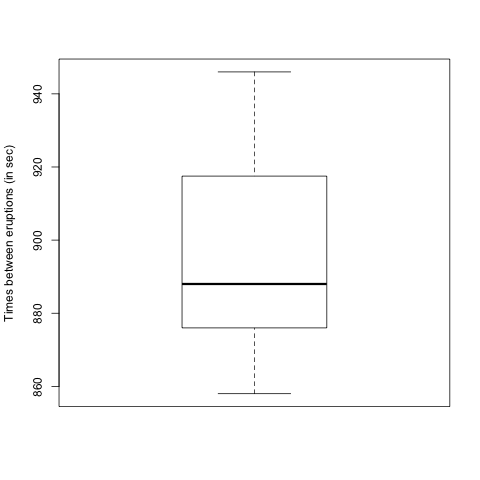
\includegraphics[width=\linewidth]{images/webwork-5-image-1.png}
}&\multicolumn{1}{c}{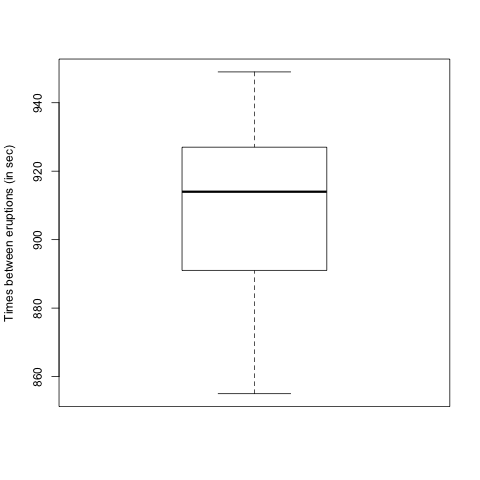
\includegraphics[width=\linewidth]{images/webwork-5-image-2.png}
}\tabularnewline[0pt]
\multicolumn{1}{c}{A}&\multicolumn{1}{c}{B}\tabularnewline[0pt]
\multicolumn{1}{c}{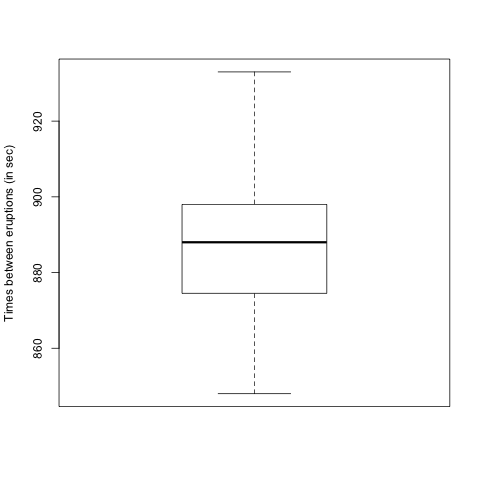
\includegraphics[width=\linewidth]{images/webwork-5-image-3.png}
}&\multicolumn{1}{c}{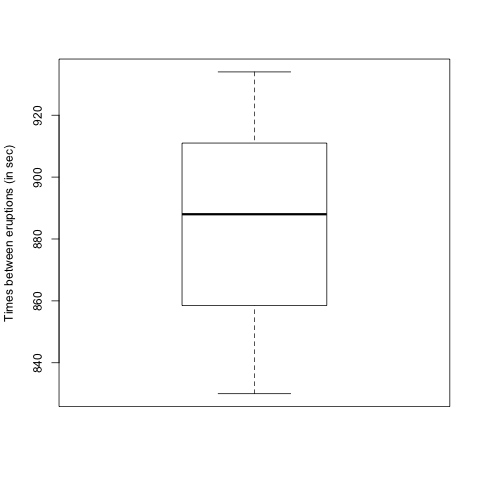
\includegraphics[width=\linewidth]{images/webwork-5-image-4.png}
}\tabularnewline[0pt]
\multicolumn{1}{c}{C}&\multicolumn{1}{c}{D}
\end{tabular}
}%
\par}
\end{sbspanel}%
\end{sidebyside}%
\par
(Click on a graph to enlarge it.)%
\par\smallskip%
\noindent\textbf{\blocktitlefont Answer 1}.\hypertarget{g:answer:idp27}{}\quad{}\(886.8\)%
\par\smallskip%
\noindent\textbf{\blocktitlefont Answer 2}.\hypertarget{g:answer:idp28}{}\quad{}\(602.029\)%
\par\smallskip%
\noindent\textbf{\blocktitlefont Answer 3}.\hypertarget{g:answer:idp29}{}\quad{}\(888\)%
\par\smallskip%
\noindent\textbf{\blocktitlefont Answer 4}.\hypertarget{g:answer:idp30}{}\quad{}\(23.5\)%
\par\smallskip%
\noindent\textbf{\blocktitlefont Answer 5}.\hypertarget{g:answer:idp31}{}\quad{}\(\text{C}\)%
\par\smallskip%
\noindent\textbf{\blocktitlefont Solution}.\hypertarget{g:solution:idp32}{}\quad{}Suppose you have entered the data in R as follows:%
\par
\(\verb| x \lt -  c( 878, 871, 906, 933, 930, 852, 890, 861, 882, 888, 897, 899, 879, 888, 848 ) |\)%
\par
Then the sample mean, sample variance, sample median, and sample IQR are obtained as follows:%
\par
\(\verb|mean(x) |\)%
\par
\(\verb|var(x) |\)%
\par
\(\verb|median(x) |\)%
\par
\(\verb|IQR(x) |\)%
\par
You can obtain a boxplot by typing%
\par
\(\verb|boxplot( x, ylab = "Times between eruptions (in sec)", id.method="y")  |\)%
\par
For the data as given, the sample mean is 886.8 sec, the variance is 602.029 min\({}^{2}\), the median is 888 min and the IQR is 23.5 min (from R's default type; it may be quite different if you used a different type.)%
\end{inlineexercise}%
Once again, we can compute these descriptive statistics using R. We again display a box and whisker diagram and you should now notice the the "box" corresponds to the IQR.%
\begin{sageinput}
data <- c( 1, -1, 0, 2, 2, 5)   # concatenate the following items into a list
print(paste("Variance = ", var(data)))
print(paste("Standard Dev = ", sd(data)))
print(paste("Inter Quantile Range =",IQR(data)))
boxplot(data, horizontal=TRUE)
\end{sageinput}
Experiment in the above interactive cell by using one of the built-in data sets.%
\par
We can also consider once again the Population of the individual USA states according to the 2013 Census is considered below.%
\begin{inlineexercise}{USA State Population Measures of Variation.}{g:exercise:idp33}%
Using the \hyperref[x:example:StatePopulations]{US Census Bureau state populations~{\xreffont\ref{x:example:StatePopulations}}} (in millions) for 2014 provided earlier, determine the range, quartiles, and variance for this sample data.%
\par\smallskip%
\noindent\hypertarget{g:solution:idp34}{}Again, you should note that these are already in order so the range is quickly found to be%
\begin{equation*}
y_n - y_1 = 38.3 - 0.6 = 37.7
\end{equation*}
million residents.%
\par
For IQR, we first must determine the quartiles. The median (found earlier) already is the second quartile so we have \(Q_2 = 4.5\) million. For the other two, the formula for computing percentiles gives you the 25th percentiile%
\begin{gather*}
(n+1)p = 51(1/4) = 12.75\\
Q_1 = P^{0.25} = 0.25 \times 1.9 + 0.75 \times 2.1 = 2.05
\end{gather*}
and the 75th percentile%
\begin{gather*}
(n+1)p = 51(3/4) = 38.25\\
Q_3 = P^{0.75} = 0.75 \times 7 + 0.25 \times 8.3 = 7.325.
\end{gather*}
Hence, the IQR = 7.325 - 2.05 = 5.275 million residents.%
\par
From the computation before, again note that n=51 since the District of Columbia is included. The mean of this data found before was found to be approximately 6.20 million residents. So, to determine the variance you may find it easier to compute using the the alternate variance formulas \hyperref[x:theorem:AlternateVariance]{Theorem~{\xreffont\ref{x:theorem:AlternateVariance}}}.%
\begin{align*}
v & = \left ( \frac{\sum_{k=1}^n y_k^2 }{n} \right ) - \mu^2\\
& \approx \frac{4434.37}{51} - (6.20)^2\\
& = 48.51
\end{align*}
and so you get a sample variance of%
\begin{equation*}
s^2 \approx \frac{51}{50} \cdot 48.51 = 49.48
\end{equation*}
and a sample standard deviation of%
\begin{equation*}
s \approx \sqrt{49.48} \approx 7.03
\end{equation*}
million residents.%
\end{inlineexercise}%
The interquartile range is sometimes also called the interquantile range. It must be noted that R computes the IQR differently for some reason. You can look up the R documentation to see what they do but notice that you can force R to use the standard approach as well.  Below, for example, the interactive cell determine the IQR using R's preferred method. However, to use the method from this text, you can make the function call IQR(data, type=2). This might be helpful to know when working on some WeBWorK exercises where the author could be using R to compute the correct answer.%
\par
The state population data set has been entered for you in the R cell below... \leavevmode%
\begin{sageinput}
data <- c (0.6,0.6,0.6,0.7,0.7,0.8,0.9,1,1.1,1.3,1.3,1.4,1.6,
1.9,1.9,2.1,2.8,2.9,2.9,3,3,3.1,3.6,3.9,3.9,4.4,4.6,
4.8,4.8,5.3,5.4,5.7,5.9,6,6.5,6.6,6.6,6.7,7,8.3,
8.9,9.8,9.9,10,11.6,12.8,12.9,19.6,19.7,26.4,38.3)
print(paste("Variance = ", var(data)))
print(paste("Standard Dev = ", sd(data)))
paste("Inter Quantile Range =",IQR(data))
\end{sageinput}
%
\end{sectionptx}
%
%
\typeout{************************************************}
\typeout{Section 1.6 Adjusting Statistical Measures for Grouped Data}
\typeout{************************************************}
%
\begin{sectionptx}{Adjusting Statistical Measures for Grouped Data}{}{Adjusting Statistical Measures for Grouped Data}{}{}{x:section:GroupedData}
\begin{introduction}{}%
As you considered the measures of the center and spread before, each data point was considered individually. Often, data may however be grouped into categories. The number of data items in each category is called the "frequency" of that outcome and the collection of these frequencies for all outcomes is called a "frequency distribution".%
\end{introduction}%
Data Grouped into Single-valued Categories%
\par
\hypertarget{x:p:GroupedDataDiscrete}{}%
Rather than considering \(x_k\) to be the kth data value, take advantage of the grouping to perhaps save a bit on arithmetic. Indeed, let's assume that data is grouped into m categories \(x_1, x_2, ..., x_m\) with corresponding frequencies \(f_1, f_2, ..., f_m\). Then, for example, when computing the mean rather than adding \(x_1\) with itself \(f_1\) times just compute \(x_1 \times f_1\) for the first category and continuing through the remaining categories. This gives the following grouped data formula for the mean%
\begin{equation*}
\mu = \frac{x_1 f_1 + ... + x_m f_m}{f_1 + ... + f_m} = \frac{\sum_{k=1}^m x_k f_k}{\sum_{k=1}^m f_k}.
\end{equation*}
and the following grouped data formula for the variance (along with one equivalent form)%
\begin{equation*}
\sigma^2 = \frac{\sum_{k=1}^m ( x_k-\mu )^2 f_k}{\sum_{k=1}^m f_k} = \frac{\sum_{k=1}^m x_k^2 f_k}{\sum_{k=1}^m f_k} - \mu^2
\end{equation*}
%
\begin{inlineexercise}{}{g:exercise:idp35}%
Consider the following data set%
\par
\textbraceleft{}3, 1, 2, 2, 3, 1, 3, 4, 5, 5, 1, 4, 5, 1, 2, 4, 5, 3, 2, 5, 2, 1, 2, 2, 5\textbraceright{}%
\par
Create a frequency distribution and determine the sample mean and variance.%
\par
\par\smallskip%
\noindentCollecting this data into a frequency distribution gives \begin{tableptx}{\textbf{Grouped Discrete Data}}{g:table:idp36}{}%
\centering
{\tabularfont%
\begin{tabular}{rr}
\(x_k\)&\(f_k\)\tabularnewline\hrulemedium
1&5\tabularnewline[0pt]
2&7\tabularnewline[0pt]
3&4\tabularnewline[0pt]
4&3\tabularnewline[0pt]
5&6
\end{tabular}
}%
\end{tableptx}%
 Therefore,%
\begin{equation*}
\overline{x} = \frac{1 \times 5 + 2 \times 7 + 3 \times 4 + 4 \times 3 + 5 \times 6}{5+7+4+3+6} \\
= \frac{5 + 14 + 12 + 12 + 30}{25} = \frac{43}{25}
\end{equation*}
and%
\begin{align*}
v & = \frac{1^2 \times 5 + 2^2 \times 7 + 3^2 \times 4 + 4^2 \times 3 + 5^2 \times 6}{5+7+4+3+6} - \left ( \frac{43}{25} \right )^2 \\
& = \frac{5 + 28 + 36 + 48 + 150}{25} - \left ( \frac{43}{25} \right )^2 \\
& = \frac{4826}{625}\\
& \approx 7.7216
\end{align*}
and so \(s^2 = \frac{25}{24} \frac{4826}{625} \approx 8.043\).%
%
\end{inlineexercise}%
\begin{inlineexercise}{WeBWorK - Grouped Discrete Data.}{g:exercise:idp37}%
The U.S. Bureau of the Census conducts nationwide surveys on characteristics of U.S. households.  Following are data on the number of people per household for a sample of 50 households.  Construct a grouped data table for these household sizes.%
\begin{sidebyside}{1}{0}{0}{0}%
\begin{sbspanel}{1}%
{\centering%
{\tabularfont%
\begin{tabular}{BlBlBlBlBlBlBlBlBlBlB}\hrulemedium
4&1&2&4&6&1&6&6&5&7\tabularnewline\hrulemedium
3&2&4&3&6&3&1&3&2&5\tabularnewline\hrulemedium
5&2&5&2&2&4&5&6&5&6\tabularnewline\hrulemedium
5&1&4&7&2&5&7&6&7&1\tabularnewline\hrulemedium
4&3&3&5&3&2&5&6&1&6\tabularnewline\hrulemedium
\end{tabular}
}%
\par}
\end{sbspanel}%
\end{sidebyside}%
\begin{sidebyside}{1}{0}{0}{0}%
\begin{sbspanel}{1}%
{\centering%
{\tabularfont%
\begin{tabular}{BlBlBlB}\hrulemedium
Household size&Frequency&Relative Frequency\tabularnewline\hrulemedium
1&\fillin{4.545454545454546}&\fillin{4.545454545454546}\tabularnewline\hrulemedium
2&\fillin{4.545454545454546}&\fillin{4.545454545454546}\tabularnewline\hrulemedium
3&\fillin{4.545454545454546}&\fillin{4.545454545454546}\tabularnewline\hrulemedium
4&\fillin{4.545454545454546}&\fillin{4.545454545454546}\tabularnewline\hrulemedium
5&\fillin{4.545454545454546}&\fillin{4.545454545454546}\tabularnewline\hrulemedium
6&\fillin{4.545454545454546}&\fillin{4.545454545454546}\tabularnewline\hrulemedium
7&\fillin{4.545454545454546}&\fillin{4.545454545454546}\tabularnewline\hrulemedium
\alert{Total}&50&1\tabularnewline\hrulemedium
\end{tabular}
}%
\par}
\end{sbspanel}%
\end{sidebyside}%
\par\smallskip%
\noindent\textbf{\blocktitlefont Answer 1}.\hypertarget{g:answer:idp38}{}\quad{}\(6\)%
\par\smallskip%
\noindent\textbf{\blocktitlefont Answer 2}.\hypertarget{g:answer:idp39}{}\quad{}\(0.12\)%
\par\smallskip%
\noindent\textbf{\blocktitlefont Answer 3}.\hypertarget{g:answer:idp40}{}\quad{}\(8\)%
\par\smallskip%
\noindent\textbf{\blocktitlefont Answer 4}.\hypertarget{g:answer:idp41}{}\quad{}\(0.16\)%
\par\smallskip%
\noindent\textbf{\blocktitlefont Answer 5}.\hypertarget{g:answer:idp42}{}\quad{}\(7\)%
\par\smallskip%
\noindent\textbf{\blocktitlefont Answer 6}.\hypertarget{g:answer:idp43}{}\quad{}\(0.14\)%
\par\smallskip%
\noindent\textbf{\blocktitlefont Answer 7}.\hypertarget{g:answer:idp44}{}\quad{}\(6\)%
\par\smallskip%
\noindent\textbf{\blocktitlefont Answer 8}.\hypertarget{g:answer:idp45}{}\quad{}\(0.12\)%
\par\smallskip%
\noindent\textbf{\blocktitlefont Answer 9}.\hypertarget{g:answer:idp46}{}\quad{}\(10\)%
\par\smallskip%
\noindent\textbf{\blocktitlefont Answer 10}.\hypertarget{g:answer:idp47}{}\quad{}\(0.2\)%
\par\smallskip%
\noindent\textbf{\blocktitlefont Answer 11}.\hypertarget{g:answer:idp48}{}\quad{}\(9\)%
\par\smallskip%
\noindent\textbf{\blocktitlefont Answer 12}.\hypertarget{g:answer:idp49}{}\quad{}\(0.18\)%
\par\smallskip%
\noindent\textbf{\blocktitlefont Answer 13}.\hypertarget{g:answer:idp50}{}\quad{}\(4\)%
\par\smallskip%
\noindent\textbf{\blocktitlefont Answer 14}.\hypertarget{g:answer:idp51}{}\quad{}\(0.08\)%
\end{inlineexercise}%
\hypertarget{x:p:GroupedDataContinuous}{}%
For measures on data grouped into intervals, it is somewhat difficult to do calculations when the data no longer exists as individual values since all you know is the frequencies of each interval. You can use "class marks"...the midpoints of each interval...as representers for all of the items that fell into that interval for computing means and variances.  For positional measures, you want to approach this in the same manner as with percentiles before.  That is, my doing some sort of linear interpolation on the width of each interval.%
\par
So, for medians, consider the following approach:  Consider data collected into intervals of the form%
\begin{itemize}[label=\textbullet]
\item{}\(\displaystyle [a_1,b_1)\)%
\item{}\(\displaystyle [a_2,b_2)\)%
\item{}\(\displaystyle [a_3,b_3)\)%
\item{}...%
\item{}\(\displaystyle [a_n,b_n)\)%
\end{itemize}
where \(f_k\) is the frequency of data items in interval \([a_k,b_k)\) with corresponding cummulative frequency \(F_k\).%
\par
%
\begin{enumerate}
\item{}Set m = total cummulative frequency\slash{}2 = \(F_{last}/2\)%
\item{}Determine the interval \(k\) where \(m \in [F_{k-1},F_k]\)%
\item{}Set median = \((b_k-a_k)\frac{m - F_{k-1}}{f_k}+a_k\)%
\end{enumerate}
%
\par
\begin{example}{Computing Median for Interval Grouped Data.}{g:example:idp52}%
\begin{tableptx}{\textbf{Interval Frequency Distribution}}{g:table:idp53}{}%
\centering
{\tabularfont%
\begin{tabular}{rr}
\([a_k,b_k]\)&\(f_k\)\tabularnewline\hrulemedium
[0,5)&5\tabularnewline[0pt]
[5,10)&7\tabularnewline[0pt]
[10,20)&4\tabularnewline[0pt]
[20,23)&3\tabularnewline[0pt]
[23,30)&6
\end{tabular}
}%
\end{tableptx}%
 The total cummulative frequency is 25 and so \(m = \frac{25}{2} = 12.5\) which lies in the k = 3 interval [10,20) and \(F_2 = 12\).  Therefore%
\begin{equation*}
\text{median} = (20-10) \frac{12.5-12}{4} + 10 = 11.25
\end{equation*}
%
\end{example}
%
\begin{inlineexercise}{Statistics using Continuous Grouped Data.}{g:exercise:idp54}%
Given the following table, compute the mean of the grouped data.%
\begin{sidebyside}{1}{0}{0}{0}%
\begin{sbspanel}{1}%
{\centering%
{\tabularfont%
\begin{tabular}{BlBlBlB}\hrulemedium
Class&Midpoint&Frequency\tabularnewline\hrulemedium
\([9,15)\)&\fillin{9.090909090909092}&\(2\)\tabularnewline\hrulemedium
\([15,21)\)&\fillin{9.090909090909092}&\(1\)\tabularnewline\hrulemedium
\([21,27)\)&\fillin{9.090909090909092}&\(9\)\tabularnewline\hrulemedium
\([27,33)\)&\fillin{9.090909090909092}&\(7\)\tabularnewline\hrulemedium
\([33,39)\)&\fillin{9.090909090909092}&\(5\)\tabularnewline\hrulemedium
\([39,45)\)&\fillin{9.090909090909092}&\(1\)\tabularnewline\hrulemedium
\([45,51)\)&\fillin{9.090909090909092}&\(0\)\tabularnewline\hrulemedium
Totals&&\fillin{9.090909090909092}\tabularnewline\hrulemedium
\end{tabular}
}%
\par}
\end{sbspanel}%
\end{sidebyside}%
\par
What is the mean of the grouped data?  \fillin{9.090909090909092}%
\par\smallskip%
\noindent\textbf{\blocktitlefont Answer 1}.\hypertarget{g:answer:idp55}{}\quad{}\(12\)%
\par\smallskip%
\noindent\textbf{\blocktitlefont Answer 2}.\hypertarget{g:answer:idp56}{}\quad{}\(18\)%
\par\smallskip%
\noindent\textbf{\blocktitlefont Answer 3}.\hypertarget{g:answer:idp57}{}\quad{}\(24\)%
\par\smallskip%
\noindent\textbf{\blocktitlefont Answer 4}.\hypertarget{g:answer:idp58}{}\quad{}\(30\)%
\par\smallskip%
\noindent\textbf{\blocktitlefont Answer 5}.\hypertarget{g:answer:idp59}{}\quad{}\(36\)%
\par\smallskip%
\noindent\textbf{\blocktitlefont Answer 6}.\hypertarget{g:answer:idp60}{}\quad{}\(42\)%
\par\smallskip%
\noindent\textbf{\blocktitlefont Answer 7}.\hypertarget{g:answer:idp61}{}\quad{}\(48\)%
\par\smallskip%
\noindent\textbf{\blocktitlefont Answer 8}.\hypertarget{g:answer:idp62}{}\quad{}\(25\)%
\par\smallskip%
\noindent\textbf{\blocktitlefont Answer 9}.\hypertarget{g:answer:idp63}{}\quad{}\(27.6\)%
\end{inlineexercise}%
\end{sectionptx}
%
%
\typeout{************************************************}
\typeout{Section 1.7 Other Statistical Point Measures}
\typeout{************************************************}
%
\begin{sectionptx}{Other Statistical Point Measures}{}{Other Statistical Point Measures}{}{}{x:section:OtherPointMeasures}
Above, we have investigated statistical measures that help determine the middle and the spread of a given data set. There are however other metrics available that help describe the distribution of that data.  Skewness is one of those metrics and describes any lack of symmetry of the data set's distribution and whether data is stretched out to one side or the other.%
\par
\begin{definition}{Skewness.}{x:definition:DefnSkewness}%
For population data, the Skewness of \(x_1, x_2, ..., x_n\) is given by%
\begin{equation*}
\frac{1}{\sigma^3} \frac{\sum_{k=1}^n ( x_k-\mu )^3}{n}.
\end{equation*}
%
\par
For sample data, the Skewness of \(x_1, x_2, ..., x_n\) is given by%
\begin{equation*}
\frac{1}{s^3} \frac{\sum_{k=1}^n ( x_k-\overline{x} )^3}{n}.
\end{equation*}
%
\end{definition}
%
\par
A positive skewness indicates that the positive \((x_k - \mu)^3\) terms (likewise \((x_k - \overline{x})^3\) terms) overwhelm the negative terms. So, a positive skewness indicates that the data set is strung out to the right. Likewise, a negative skewness indicates a data set that is strung out to the left.%
\par
Data might tend to be clustered around the mean. The "kurtosis" can be used to measure how closely data resembles a "bell-shaped" collection.%
\par
\begin{definition}{Kurtosis.}{x:definition:DefnKurtosis}%
For population data, the Kurtosis of \(x_1, x_2, ..., x_n\) is given by%
\begin{equation*}
\frac{1}{\sigma^4} \frac{\sum_{k=1}^n ( x_k-\mu )^4}{n}.
\end{equation*}
%
\par
For sample data, the Kurtosis of \(x_1, x_2, ..., x_n\) is given by%
\begin{equation*}
\frac{1}{s^4} \frac{\sum_{k=1}^n ( x_k-\overline{x} )^4}{n}.
\end{equation*}
%
\end{definition}
%
\par
A kurtosis of 3 indicates that the data is perfectly bell shaped (a "normal" distribution) whereas data further away from 3 indicates data that is less bell shaped.%
\begin{theorem}{Alternate Formulas for Skewness and Kurtosis.}{}{x:theorem:AlternateSkewnessAndKurtosis}%
Skewness =%
\begin{equation*}
\text{skewness} = \frac{1}{s^3} 
\left [ \frac{\sum_{k=1}^n x_k^3}{n} - 3 \overline{x}\sum_{k=1}^n \frac{x_k^2}{n} + 2 \overline{x}^3 \right ]
\\ = \frac{1}{s^3} 
\left [ \frac{\sum_{k=1}^n x_k^3}{n} - 3 v \overline{x} - \overline{x}^3 \right ]
\end{equation*}
and Kurtosis =%
\begin{equation*}
\text{kurtosis}  = \frac{1}{s^4} 
\left [ 
\frac{\sum_{k=1}^n x_k^4}{n} - 4 \overline{x} \frac{\sum_{k=1}^n x_k^3 }{n} + 6 \overline{x}^2 \frac{\sum_{k=1}^n x_k^2}{n} - 3 \overline{x}^4  \right ]
\\ = \frac{1}{s^4} \left [ \frac{\sum_{k=1}^n x_k^4}{n} - 4 \overline{x} \frac{\sum_{k=1}^n x_k^3 }{n} + 6 \overline{x}^2 v + 3 \overline{x}^4  
\right ]
\end{equation*}
\begin{proof}{}{g:proof:idp64}
For skewness, expand the cubic and break up the sum. Factoring out constants (such as \(\overline{x}\)) gives%
\begin{align*}
& \frac{\sum_{k=1}^n ( x_k-\overline{x} )^3}{n}\\
& = \frac{\sum_{k=1}^n x_k^3}{n} - 3 \overline{x} \frac{\sum_{k=1}^n x_k^2 }{n} + 3 \overline{x}^2 \frac{\sum_{k=1}^n x_k}{n} - \frac{\sum_{k=1}^n \overline{x}^3}{n}\\
& = \frac{\sum_{k=1}^n x_k^3}{n} - 3 \overline{x}(v + \overline{x}^2) + 3 \overline{x}^3 - \overline{x}^3\\
& = \frac{\sum_{k=1}^n x_k^3}{n} - 3 \overline{x}v - \overline{x}^3
\end{align*}
and divide by the cube of the standard deviation to finish. Note that the first expansion in the derivation above can be used quickly if the data is collected in a table and powers easily computed.%
\par
For kurtosis, similarly expand the quartic and break up the sum as before. Note that you can extract the value of the cubic term by solving for that term in the skewness formula above. Then,%
\begin{align*}
& \frac{\sum_{k=1}^n ( x_k-\overline{x} )^4}{n}\\
& = \frac{\sum_{k=1}^n x_k^4}{n} - 4 \overline{x} \frac{\sum_{k=1}^n x_k^3 }{n} + 6 \overline{x}^2 \frac{\sum_{k=1}^n x_k^2}{n} - 4 \overline{x}^3 \frac{\sum_{k=1}^n x_k}{n} + \frac{\sum_{k=1}^n \overline{x}^4}{n}\\
& = \frac{\sum_{k=1}^n x_k^4}{n} - 4 \overline{x} \frac{\sum_{k=1}^n x_k^3 }{n} + 6 \overline{x}^2 (v+\overline{x}^2) - 4 \overline{x}^4 + \overline{x}^4\\
& = \frac{\sum_{k=1}^n x_k^4}{n} - 4 \overline{x} \frac{\sum_{k=1}^n x_k^3 }{n} + 6 \overline{x}^2 v + 3 \overline{x}^4 
\end{align*}
and then divide by the fourth power of the standard deviation.  Note again that the first expansion in the derivation above might also be a useful shortcut.%
\end{proof}
\end{theorem}
It should be noted that there are other possible ways to come up with interesting alternate ways to compute the kurtosis, etc. based on previous values. The ones presented above relate back to the mean and variance whose values might be more readily obtained from calculators for example.%
\par
Going back to a previous example...%
\par
Computing skewness and kurtosis by hand can often be better organized using a table. Below, notice that the \(x_k\) column would be the given data values but the other columns you could again easily compute. \begin{tableptx}{\textbf{Computing data statistics by hand}}{g:table:idp65}{}%
\centering
{\tabularfont%
\begin{tabular}{rrrr}
\(x_k\)&\(x_k^2\)&\(x_k^3\)&\(x_k^4\)\tabularnewline\hrulemedium
1&1&1&1\tabularnewline[0pt]
-1&1&-1&1\tabularnewline[0pt]
0&0&0&0\tabularnewline[0pt]
2&4&8&16\tabularnewline[0pt]
2&4&8&16\tabularnewline[0pt]
5&25&125&625
\end{tabular}
}%
\end{tableptx}%
 So, \(\Sigma x_k = 9\) and \(\Sigma x_k^2 = 35\) as before and so%
\begin{equation*}
\overline{x} = \frac{9}{6} = \frac{3}{2}
\end{equation*}
and%
\begin{gather*}
v = \frac{25}{6} - \left ( \frac{3}{2} \right )^2 = \frac{43}{12} \approx 3.58 ,\\
s^2 = \frac{6}{5} \times v = \frac{43}{10} = 4.3,\\
\text{and so} s = \sqrt{4.3} \approx 2.07\text{.}
\end{gather*}
But also, \(\Sigma x_k^3 = 141\) and \(\Sigma x_k^4 = 659\).  Use these in the formulas above to obtain skewness of%
\begin{equation*}
\left [ \frac{141}{6} - 3 \cdot \frac{26}{5} \cdot \frac{3}{2} - \left ( \frac{3}{2} \right )^2 \right ] / s^3 
\end{equation*}
and kurtosis of%
\begin{equation*}
\left [ \frac{659}{6} - 4 \cdot \frac{3}{2} \cdot \frac{141}{6} + 6 \left ( \frac{3}{2} \right )^2  \cdot \frac{26}{5}  - 3 \cdot \left ( \frac{3}{2} \right )^4 \right ] / s^4.
\end{equation*}
%
\end{sectionptx}
%
%
\typeout{************************************************}
\typeout{Section 1.8 Visual Statistical Measures - Graphical Representation of Data}
\typeout{************************************************}
%
\begin{sectionptx}{Visual Statistical Measures - Graphical Representation of Data}{}{Visual Statistical Measures - Graphical Representation of Data}{}{}{x:section:GraphicalStatistics}
\begin{introduction}{}%
Data sets can range from small to very large. Visual representations of these data sets often allow you to see trends and reveal a lot about the distribution of the data values. Several ways to describe data using graphical means are presented below.%
\end{introduction}%
\hypertarget{x:p:GraphicalStatisticsHistograms}{}%
 Often the quantity of data available makes it difficult to see trends and general relationships within the data. As the saying goes "A picture is worth a thousand words" and one way to express data with a picture is with a bar chart called a "histogram".  Most gnerally, histograms describe frequencies or relative frequencies and are more specifically described with additional modifers such as "relative frequence histogram".%
\par
Frequency Histograms - height matters%
\par
Consider the data set given by \begin{tableptx}{\textbf{Basic Frequency Table}}{g:table:idp66}{}%
\centering
{\tabularfont%
\begin{tabular}{rr}
\(x_k\)&\(f_k\)\tabularnewline\hrulemedium
1&8\tabularnewline[0pt]
2&12\tabularnewline[0pt]
3&6\tabularnewline[0pt]
4&3\tabularnewline[0pt]
5&1\tabularnewline[0pt]
6&2
\end{tabular}
}%
\end{tableptx}%
%
\par
A frequency histogram representing this data looks like \begin{image}{0}{1}{0}%
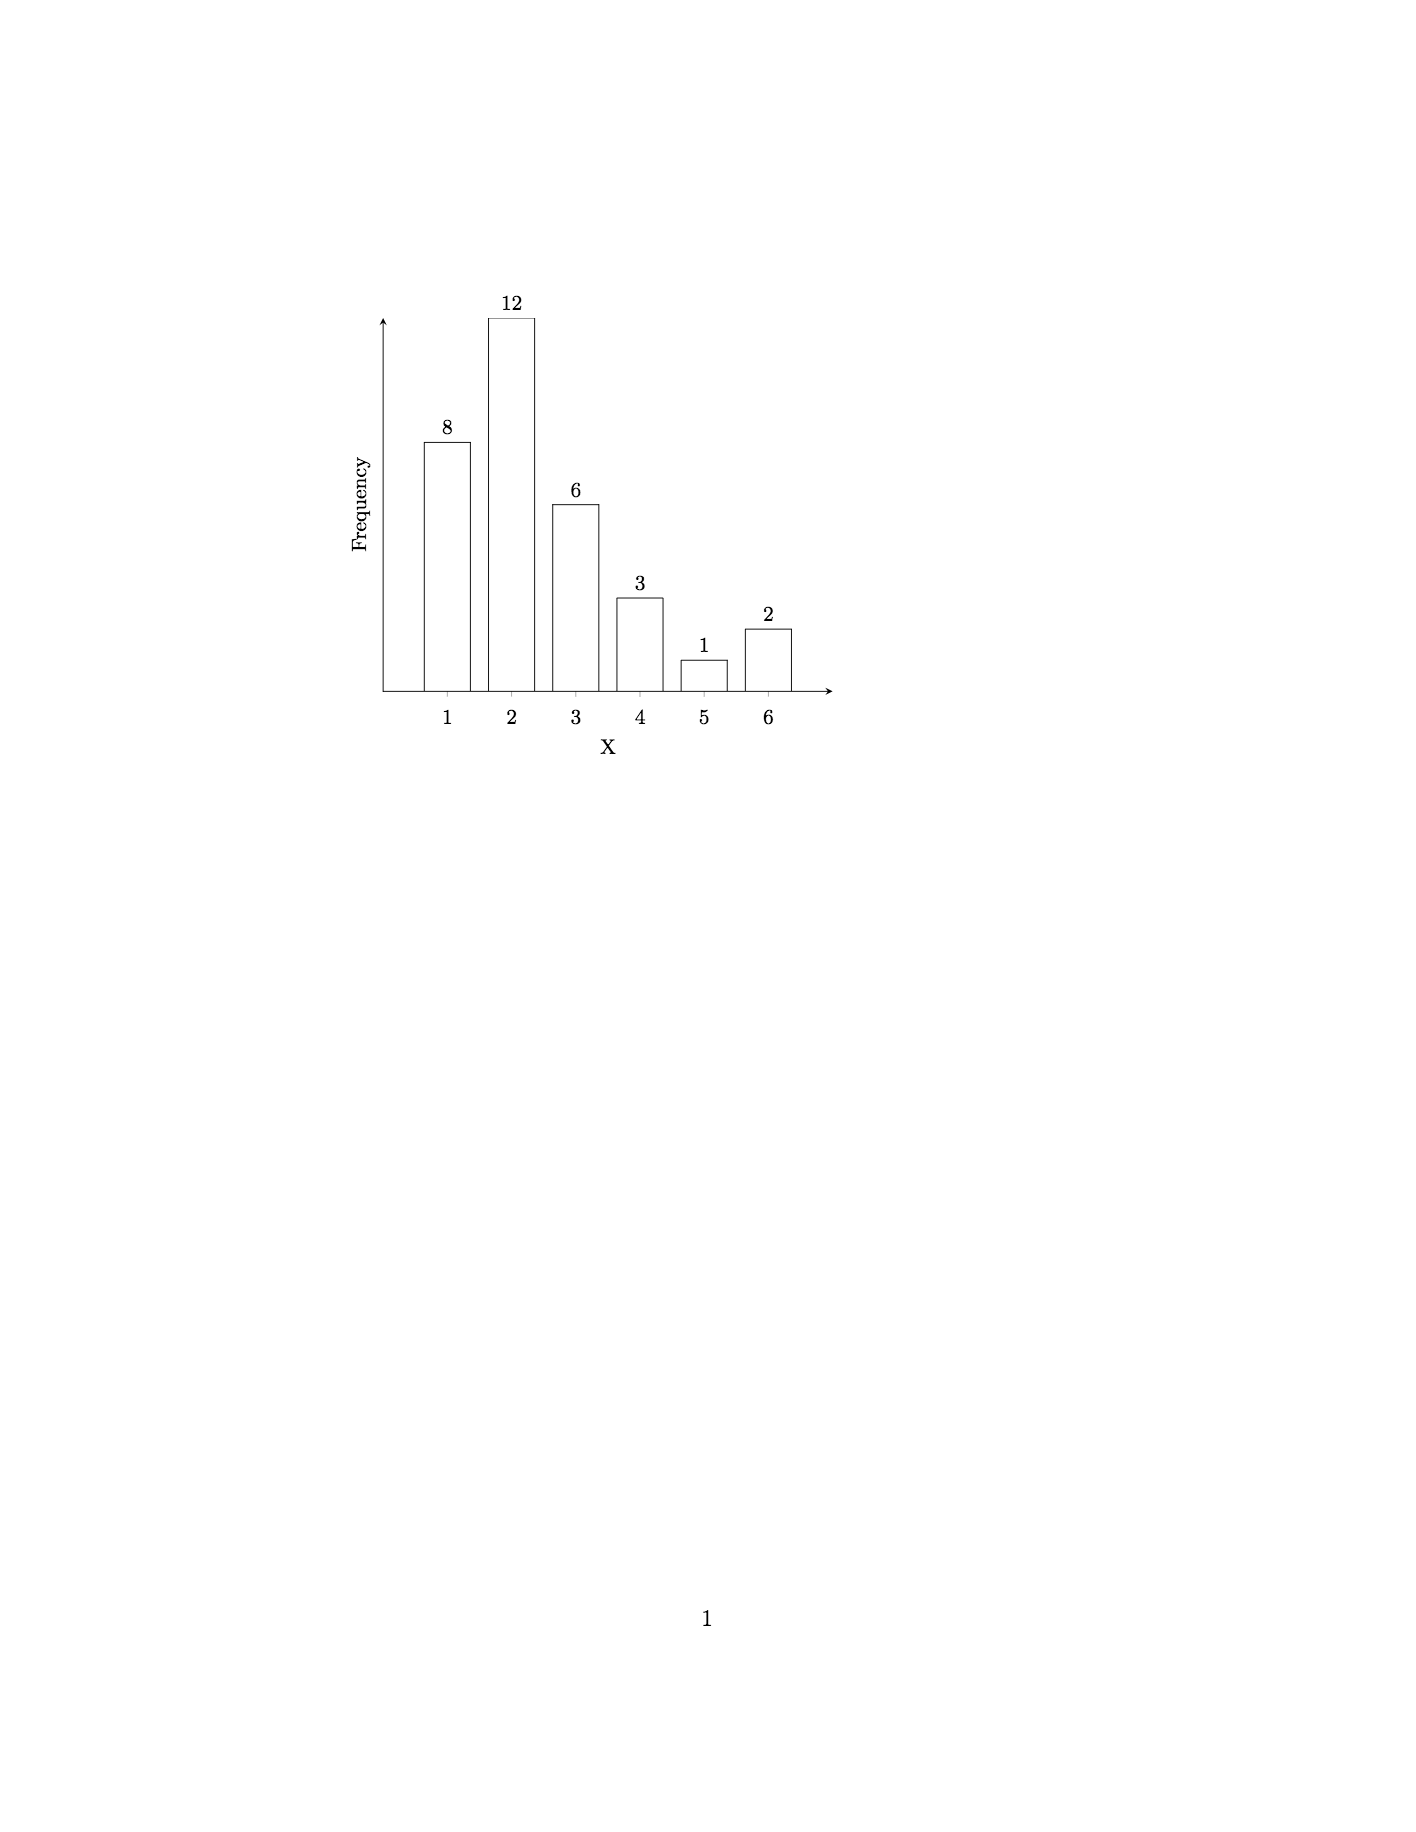
\includegraphics[width=\linewidth]{images/frequencyhistogram.png}
\end{image}%
%
\par
Experiment with creating your own histogram by inputting your data into the interactive Sage cell below. \leavevmode%
\begin{sageinput}
#  This function is used to convert an input string into separate entries
def g(s): return str(s).replace(',',' ').replace('(',' ').replace(')',' ').split()

@interact
def _(freq = input_box("1,1,1,1,2,2,2,3,3,3,3,1,5",label="Enter data separated by commas")):
    freq = g(freq)
    freq = [int(k) for k in freq]
    m = min(freq)
    M = max(freq)
    bn = M-m+1
    histogram( freq, range=[m-1/2,M+1/2], bins = bn, align="mid", linewidth=2, edgecolor="blue", color="yellow").show()
\end{sageinput}
%
\par
Relative Frequency Histograms - In this case, area describes relative frequency.  Notice in the interactive cell above that each bar is of width one. Therefore, frequency = area. In some instances where data may be grouped the total width of the interval may be different and so the height will need to be adjusted so that the total area of each bar corresponds to the relative frequency of that category.%
\par
Cummulative Histograms.  In these a running total is presented using all values from the given point and below.%
\begin{sageinput}
#  This function is used to convert an input string into separate entries
def g(s): return str(s).replace(',',' ').replace('(',' ').replace(')',' ').split()

@interact
def _(freq = input_box("1,1,1,1,2,2,2,3,3,3,3,1,5",label="Enter data separated by commas")):
    freq = g(freq)
    freq = [int(k) for k in freq]
    top = len(freq)
    m = min(freq)
    M = max(freq)
    bn = M-m+1
    histogram( freq, range=[m-1/2,M+1/2], cumulative = "true", bins = bn, align="mid", linewidth=2, edgecolor="blue", color="yellow").show(ymax=top)
\end{sageinput}
\hypertarget{x:p:GraphicalStatisticsStemAndLeaf}{}%
 A Stem and Leaf Plot allows you to create a histogram of sorts but maintain the individual data values. To create one of these plots, you will need to consider your particular data set and create a two-step sieve for organizing the set.  The first part is to create "stems" that are often associated with the highest digit(s) of each data value and the "leaves" that are often associated with the remaining digit(s) of the data value.%
%
\par
Once the data set is broken down into stems and leaves, it is often simple to sort the leaves under each stem to yield an "ordered Stem and Leaf Plot". Such as mechanism is a simple two-step procedure that allows you to sort a data set by hand.%
\par
\begin{example}{Simple Stem and Leaf Plot.}{g:example:idp67}%
Consider the data points 25, 3, 17, 12, 22, 34, 12, 11, 16, 42, 9, 12, 17. In this case we will consider the stems to be the tens digits and the leaves to be the ones digits. This gives%
\par
\begin{tableptx}{\textbf{Stem and Leaf Plot (unordered)}}{g:table:idp68}{}%
\centering
{\tabularfont%
\begin{tabular}{rr}
Stems&Leaves\tabularnewline\hrulemedium
0&\multicolumn{1}{l}{3 9}\tabularnewline[0pt]
1&\multicolumn{1}{l}{7 2 2 1 6 2 7}\tabularnewline[0pt]
2&\multicolumn{1}{l}{5 2}\tabularnewline[0pt]
3&\multicolumn{1}{l}{4}\tabularnewline[0pt]
4&\multicolumn{1}{l}{2}
\end{tabular}
}%
\end{tableptx}%
 Then, an ordered Stem and Leaf Plot would be \begin{tableptx}{\textbf{Stem and Leaf Plot (ordered)}}{g:table:idp69}{}%
\centering
{\tabularfont%
\begin{tabular}{rr}
Stems&Leaves\tabularnewline\hrulemedium
0&\multicolumn{1}{l}{3 9}\tabularnewline[0pt]
1&\multicolumn{1}{l}{1 2 2 2 6 7 7}\tabularnewline[0pt]
2&\multicolumn{1}{l}{2 5}\tabularnewline[0pt]
3&\multicolumn{1}{l}{4}\tabularnewline[0pt]
4&\multicolumn{1}{l}{2}
\end{tabular}
}%
\end{tableptx}%
%
\par
Notice, in each case you can extract the original data values by recombining the stem with a corresponding leaf. Indeed, for these 13 data values the median should be be 7th in the sorted list or the value in the 10's stem with leaf 6...that is, 16.%
\end{example}
%
\par
\begin{example}{Stem and Leaf Plot for State Populations.}{g:example:idp70}%
Using the state population data above, consider organizing the data but using a "two-pass sort" where you first roughly break data up into groups based upon ranges which relate to their first digit(s). In this case, let's break up into groups according to populations corresponding to 0-4 million, 5-9 million, 10-14 million, 15-19, million, 20-24 million, 25-29 million, 30-35 million, and 35-39 million. We can represent these classes by using the stems 0L, 0H, 1L, 1H, 2L, 2H, 3L, and 3H where the L and H represent the one's digits L in \textbraceleft{}0, 1, 2, 3, 4\textbraceright{} and H in \textbraceleft{}5, 6, 7, 8, 9\textbraceright{}.  Once we group the data into these smaller groups then we can write the remaining portion of the number horizontally as leaves (in this case with one decimal place for all values.) This gives a step-and-leaf plot. If we additionally sort the data in the leaves then this gives you an ordered stem-and-leaf plot. For the state population data, the ordered stem-and-leaf plot is given by \begin{image}{0}{1}{0}%
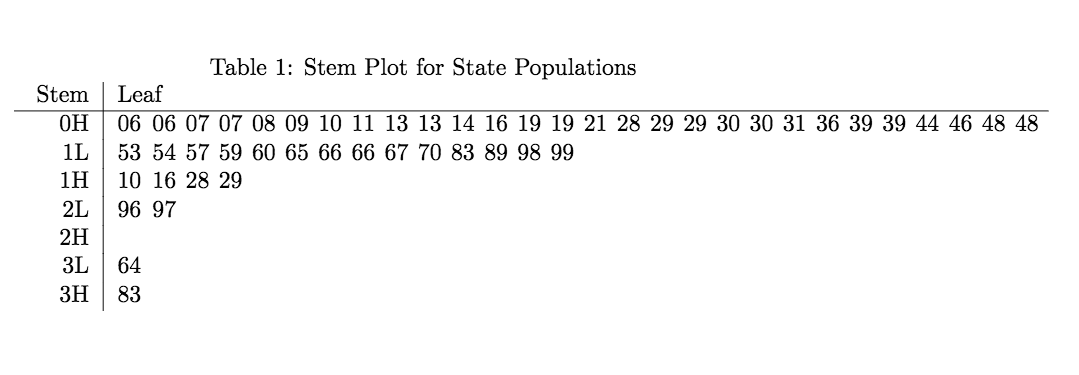
\includegraphics[width=\linewidth]{images/stemandleaf.png}
\end{image}%
 Notice how it is easy to now see that most state populations are relatively small and that there are relatively few states with larger population. Also, notice that you can use this plot to relatively easily identify minimum, maximum, and other order statistics.%
\end{example}
%
\par
\hypertarget{x:p:GraphicalStatisticsBoxAndWhisker}{}%
 This graphical display identifies the \hyperref[x:definition:DefnFiveNumberSummary]{5-number-summary~{\xreffont\ref{x:definition:DefnFiveNumberSummary}}} associated with the minimum, \hyperref[x:definition:DefnQuartiles]{quartiles~{\xreffont\ref{x:definition:DefnQuartiles}}}, and the maximum. That is, \(y_1, Q_1, Q_2, Q_3, y_n\).  These values separate the data roughly into quarters. To distinguish these quarters connect \(y_1\) and \(Q_1\) with a straight line (a whisker) and do the same with \(Q_3\) and \(y_n\). Use a box to connect \(Q_1\) with \(Q_2\) and the same to connect \(Q_2\) with \(Q_3\). Then the boxed areas also identify the IQR.%
%
\par
\leavevmode%
\begin{sageinput}
data <- c (0.6,0.6,0.6,0.7,0.7,0.8,0.9,1,1.1,1.3,1.3,
1.4,1.6,1.9,1.9,2.1,2.8,2.9,2.9,3,3,3.1,
3.6,3.9,3.9,4.4,4.6,4.8,4.8,5.3,5.4,5.7,
5.9,6,6.5,6.6,6.6,6.7,7,8.3,8.9,9.8,9.9,
10,11.6,12.8,12.9,19.6,19.7,26.4,38.3)
paste("Inter Quantile Range =",IQR(data))
paste("Box and Whisker Diagram - Box Plot):")
boxplot(data, horizontal=TRUE)
\end{sageinput}
%
\begin{inlineexercise}{WeBWorK - Computing Percentiles.}{g:exercise:idp71}%
Consider the following box and whisker plot.  Find the indicated values of the represented data.%
\begin{sidebyside}{1}{-0.083333333333335}{-0.083333333333335}{0}%
\begin{sbspanel}{1.16666666666667}%
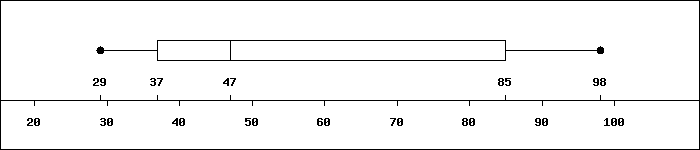
\includegraphics[width=\linewidth]{images/webwork-8-image-1.png}
\end{sbspanel}%
\end{sidebyside}%
\par
Minimum: \fillin{2.272727272727273}%
\par
Maximum: \fillin{2.272727272727273}%
\par\smallskip%
\noindent\textbf{\blocktitlefont Answer 1}.\hypertarget{g:answer:idp72}{}\quad{}\(29\)%
\par\smallskip%
\noindent\textbf{\blocktitlefont Answer 2}.\hypertarget{g:answer:idp73}{}\quad{}\(98\)%
\end{inlineexercise}%
\end{sectionptx}
%
%
\typeout{************************************************}
\typeout{Section 1.9 Summary}
\typeout{************************************************}
%
\begin{sectionptx}{Summary}{}{Summary}{}{}{x:section:RepresentingDataSummary}
Links to the main formulas related to descriptive statistics:%
\par
\hyperref[x:definition:DefnOrderStatistics]{Order Statistics~{\xreffont\ref{x:definition:DefnOrderStatistics}}}%
\par
\hyperref[x:definition:DefnMaxMin]{Maximum and Minimum~{\xreffont\ref{x:definition:DefnMaxMin}}}%
\par
\hyperref[x:definition:DefnPercentiles]{Percentiles~{\xreffont\ref{x:definition:DefnPercentiles}}}%
\par
\hyperref[x:definition:DefnQuartiles]{Quartiles~{\xreffont\ref{x:definition:DefnQuartiles}}}%
\par
\hyperref[x:definition:DefnDeciles]{Deciles~{\xreffont\ref{x:definition:DefnDeciles}}}%
\par
\hyperref[x:definition:DefnFiveNumberSummary]{5-number summary~{\xreffont\ref{x:definition:DefnFiveNumberSummary}}}%
\par
\hyperref[x:definition:DefnMean]{Mean~{\xreffont\ref{x:definition:DefnMean}}}%
\par
\hyperref[x:definition:DefnMedian]{Median~{\xreffont\ref{x:definition:DefnMedian}}}%
\par
\hyperref[x:definition:DefnMidrange]{Midrange~{\xreffont\ref{x:definition:DefnMidrange}}}%
\par
\hyperref[x:definition:DefnRange]{Range~{\xreffont\ref{x:definition:DefnRange}}}%
\par
\hyperref[x:definition:DefnIQR]{Inter Quartile Range~{\xreffont\ref{x:definition:DefnIQR}}}%
\par
\hyperref[x:definition:DefnVarianceSD]{Variance~{\xreffont\ref{x:definition:DefnVarianceSD}}}%
\par
\hyperref[x:definition:DefnSkewness]{Skewness~{\xreffont\ref{x:definition:DefnSkewness}}}%
\par
\hyperref[x:definition:DefnKurtosis]{Kurtosis~{\xreffont\ref{x:definition:DefnKurtosis}}}%
\end{sectionptx}
%
%
\typeout{************************************************}
\typeout{Section 1.10 Exercises}
\typeout{************************************************}
%
\begin{sectionptx}{Exercises}{}{Exercises}{}{}{x:section:RepresentingDataExercises}
Complete the online WebWorK homework set "Computational Measures".%
\begin{inlineexercise}{}{g:exercise:idp74}%
Create a data set with about 10 elements. For your data set, compute each of the measures from this chapter and present your data using a frequency histogram.%
\end{inlineexercise}%
\begin{inlineexercise}{}{g:exercise:idp75}%
Find a "real-world" data set (similar perhaps to the Census data presented above.) Compute each of the measures from this chapter. Interpret and present your conclusions in an electronic report which can include an excel spreadsheet.%
\end{inlineexercise}%
\end{sectionptx}
\end{chapterptx}
%
%
\typeout{************************************************}
\typeout{Chapter 2 Regression}
\typeout{************************************************}
%
\begin{chapterptx}{Regression}{}{Regression}{}{}{x:chapter:Regression}
%
%
\typeout{************************************************}
\typeout{Section 2.1 Introduction}
\typeout{************************************************}
%
\begin{sectionptx}{Introduction}{}{Introduction}{}{}{x:section:RegressionIntroduction}
Given two distinct points, there is one line which passes exactly through both.  Indeed, if the points are \((x_1,y_1), (x_2,y_2)\) then presuming the x-values are different gives the equation%
\begin{equation*}
y = \frac{y_2 - y_1}{x_2 - x_1}(x - x_1) + y_1
\end{equation*}
is the linear function which passes through both points.  If the x's are equal then%
\begin{equation*}
x = x_1
\end{equation*}
is your linear equation. However, once you collect three or more points it is likely that there is no line which exactly "interpolates" all of the points.%
\par
In this chapter, you will investigate how to create polynomial functions which in some manner approximate a collection of data point in some "best" manner.%
\end{sectionptx}
%
%
\typeout{************************************************}
\typeout{Section 2.2 Best-fit Line}
\typeout{************************************************}
%
\begin{sectionptx}{Best-fit Line}{}{Best-fit Line}{}{}{x:section:BestFitLine}
In this section, we will presume only one independent variable x and one dependent variable y.%
\par
Consider a collection of data points%
\begin{equation*}
(x_1,y_1), (x_2,y_2), ... , (x_n,y_n)
\end{equation*}
and a general linear function%
\begin{equation*}
f(x) = mx + b.
\end{equation*}
It is possible that each of the given data points are exactly "interpolated" by the linear function so that%
\begin{equation*}
f(x_k) = y_k
\end{equation*}
for k = 1, 2, ... , n.  However, in general this is unlikely since even three points are not likely to be colinear. However, you may notice that the data points exhibit a linear tendency or that the underlying physics might suggest a linear model. If so, you may find it easier to predict values of y for given values of x using a linear approximation. Here you will investigate a method for doing so called "linear regression", "least-squares", or "best-fit line".%
\par
But why even bother creating a formula (a line here) to approximate data that does not satisfy that formula? Remember that you would expect collected data to vary slightly as one repeatedly collects that data in the same way that you would expect to make a slightly different score on repeated attempts at exams on the same material. Creating a forumla that is close to your data gives a well-defined way to predict a y value for a given x value. This predictive behavior is illustrated in the exercise below.%
\begin{inlineexercise}{WeBWorK - best-fit line for approximation.}{g:exercise:idp76}%
An train station has determined that the relationship between the number of passengers on a train and the total weight of luggage stored in the baggage compartment can be estimated by the least squares regression equation \(y = 177 + 24 x\). Predict the weight of luggage for a flight with 148 passengers.%
\par
Answer: \fillin{6.818181818181818} pounds%
\par\smallskip%
\noindent\textbf{\blocktitlefont Answer}.\hypertarget{g:answer:idp77}{}\quad{}\(3729\)%
\end{inlineexercise}%
To determine the best-fit line, you need to determine what is meant by the word "best". Here, we will derive the standard approach which interprets this to mean that the total vertical error between the line and the provided data points is minimized in some fashion.  Indeed, this vertical error would be of the form%
\begin{equation*}
e_k = f(x_k) - y_k
\end{equation*}
and would be zero if f(x) exactly interpolated at the given data point.  Note, some of these errors will be positive and some will be negative. To avoid any possible cancellation of errors, you can look at taking absolute values (which is tough to deal with algebraically) or by squaring the errors. This second option will be the approach taken here. This is similar to the approach taken earlier when developing formulas for the variance.%
\par
The best-fit line therefore will be the line \(f(x) = mx+b\) so that the "total squared error" is minimized. This total squared error is given by%
\begin{equation*}
TSE(m,b) = \sum_{k=1}^n e_k^2 = \sum_{k=1}^n (f(x_k) - y_k)^2 = \sum_{k=1}^n (m x_k + b - y_k)^2.
\end{equation*}
%
\par
For the following interactive cell, consider for the given data points various values for the slope and y-intercept and see if you can make the total squared error as small as possible. In doing so, notice the vertical distances from the line to the given data points generally decreases as this error measure gets smaller.%
\begin{sageinput}
var('x')
@interact
def _(Points = input_box([(-1,1),(3,1),(4,3),(6,4)]), m = slider(-4,4,0.05,1),b = slider(-2,2,0.05,1)):   
    G = points(Points,size=20)
    xpt = []
    ypt = []
    f = m*x + b
    TSE = 0
    for k in range(len(Points)):
        x0 = Points[k][0]
        xpt.append(x0)
        y0 = Points[k][1]
        ypt.append(y0)
        TSE += (f(x=x0) - y0)^2
        G += line([(x0,f(x=x0)),(x0,y0)],color='orange')
    G += plot(f,x,min(xpt),max(xpt),color='gray')
    T = 'Total Squared Error = $%s$'%str(TSE)
    G.show(title = T)
\end{sageinput}
So that we don't have to guess the best values for slope and intercept, we can appeal to calculus. Indeed, to minimize this function of the two variables m and b take partial derivatives and set them equal to zero to get the critical values:%
\begin{equation*}
TSE_m = \sum_{k=1}^n 2(m x_k + b - y_k) \cdot x_k
\end{equation*}
and%
\begin{equation*}
TSE_b = \sum_{k=1}^n 2(m x_k + b - y_k) \cdot 1 .
\end{equation*}
Setting equal to zero and solving gives what is known as the "normal equations":%
\begin{equation*}
m \sum_{k=1}^n x_k^2 + b \sum_{k=1}^n x_k = \sum_{k=1}^n x_k y_k
\end{equation*}
and%
\begin{equation*}
m \sum_{k=1}^n x_k + b \sum_{k=1}^n 1 = \sum_{k=1}^n y_k.
\end{equation*}
Solving these for m and b gives the best fit line.%
\begin{inlineexercise}{WeBWorK - Best fit line.}{g:exercise:idp78}%
A study was conducted to detemine whether a the final grade of a student in an introductory psychology course is linearly related to his or her performance on the verbal ability test administered before college entrance.  The verbal scores and final grades for \(10\) students are shown in the table below.%
\begin{sidebyside}{1}{0}{0}{0}%
\begin{sbspanel}{1}%
{\centering%
{\tabularfont%
\begin{tabular}{BlBlBlB}\hrulemedium
Student&Verbal Score \(x\)&Final Grade \(y\)\tabularnewline\hrulemedium
\(1\)&\(31\)&\(38\)\tabularnewline\hrulemedium
\(2\)&\(77\)&\(91\)\tabularnewline\hrulemedium
\(3\)&\(68\)&\(84\)\tabularnewline\hrulemedium
\(4\)&\(40\)&\(48\)\tabularnewline\hrulemedium
\(5\)&\(76\)&\(93\)\tabularnewline\hrulemedium
\(6\)&\(77\)&\(88\)\tabularnewline\hrulemedium
\(7\)&\(32\)&\(39\)\tabularnewline\hrulemedium
\(8\)&\(36\)&\(39\)\tabularnewline\hrulemedium
\(9\)&\(44\)&\(53\)\tabularnewline\hrulemedium
\(10\)&\(46\)&\(59\)\tabularnewline\hrulemedium
\end{tabular}
}%
\par}
\end{sbspanel}%
\end{sidebyside}%
\par
Find the least squares line.%
\par
\(\hat{y} =\) \fillin{4.545454545454546} \(+\) \fillin{4.545454545454546} \(x\)%
\par
Should the regression be used to predict the final grade of a student with a verbal score of 100?%
\par
answer: \fillin{4.545454545454546}%
\par\smallskip%
\noindent\textbf{\blocktitlefont Answer 1}.\hypertarget{g:answer:idp79}{}\quad{}\(0.717328340306011\)%
\par\smallskip%
\noindent\textbf{\blocktitlefont Answer 2}.\hypertarget{g:answer:idp80}{}\quad{}\(1.18562944325795\)%
\par\smallskip%
\noindent\textbf{\blocktitlefont Answer 3}.\hypertarget{g:answer:idp81}{}\quad{}no%
\end{inlineexercise}%
\end{sectionptx}
%
%
\typeout{************************************************}
\typeout{Section 2.3 Correlation}
\typeout{************************************************}
%
\begin{sectionptx}{Correlation}{}{Correlation}{}{}{x:section:Correlation}
You can plot points and plot the resulting best-fit line determined in the previous section but the question remains whether the line is any good. In particular, the real use of the line often is to subsequently predict y-values for a given x-value. However, it is very likely that the best-fit line does not even pass through any of the provided data points.  So, how can something that misses every marker still be considered a good fit. To quantify this, we first need to discuss a way to measure how well two variables vary with each other.%
\begin{definition}{Sample Covariance.}{x:definition:DefnSampleCovariance}%
Given paired data%
\begin{equation*}
(x_1,y_1), (x_2,y_2), ... , (x_n,y_n)
\end{equation*}
with corresponding means \(\overline{x}\) and \(\overline{y}\), the sample covariance is given by%
\begin{equation*}
s_{xy} = \sum_{k=1}^n \frac{(x_k-\overline{x})(y_k-\overline{y})}{n-1}.
\end{equation*}
%
\end{definition}
This general definition provides a general measure which is a second order term (like variance) but also maintains "units". To provide a unit-less metric, consider the following measure.%
\begin{definition}{Spearman's Rho (Correlation Coefficient).}{x:definition:DefnCorrelationCoefficient}%
Given a collection of data points, the Spearman's Rho correlation coefficient is given by%
\begin{equation*}
r = \frac{s_{xy}}{s_x s_y}
\end{equation*}
where \(s_x\) is the standard deviation of the x-values only and \(s_y\) is the standard deviation of the y-values only.%
\end{definition}
\begin{theorem}{Interpretation of the Spearman's Rho Correlation Coefficient.}{}{g:theorem:idp82}%
If the points are co-linear with a positive slope then r = 1 and if the points are co-linear with a negative slope then r = -1.\end{theorem}
\begin{proof}{}{g:proof:idp83}
Assume the data points are co-linear with a positive slope. Then the%
\begin{equation*}
TSE(m_0,b_0) = 0
\end{equation*}
for some \(m_0\) and \(b_0\). For this line notice that \(f(x_k) = y_k\) exactly for all data points. It is easy to show then that%
\begin{equation*}
\overline{y} = m_0 \overline{x} + b_0
\end{equation*}
and%
\begin{equation*}
s_y = | m_0 | s_x\text{.}
\end{equation*}
Therefore,%
\begin{equation*}
s_{xy} = \sum_{k=1}^n \frac{(x_k - \overline{x})(m_0 x_k + b_0 - (m_0 \overline{x} + b_0))}{n-1} = m_0 s_x^2
\end{equation*}
Putting these together gives correlation coefficient%
\begin{equation*}
r = \frac{m_0 s_x^2}{s_x m_0 s_x} = 1.
\end{equation*}
A similar proof follows in the second case by noting that%
\begin{equation*}
m_0 / | m_0 | = -1.\qedhere
\end{equation*}
%
\end{proof}
\begin{theorem}{Alternate formula for r.}{}{g:theorem:idp84}%
%
\begin{equation*}
s_{xy} = \frac{n}{n-1} \left [ \frac{\sum_{k=1}^n x_k y_k}{n} - \overline{x} \overline{y} \right ].
\end{equation*}
%
\end{theorem}
\begin{proof}{}{g:proof:idp85}
Expand \((x_k-\overline{x})(y_k-\overline{y})\) and notice that the sample means are actually constants with respect to the summation.%
\end{proof}
To compute the best-fit line and correlation coefficient by hand, it is often easiest to construct a table in a manner similar to how you might have computed the mean, variance, skewness and kurtosis in the previous chapter.  Indeed, \begin{tableptx}{\textbf{Computing best fit line and correlation coefficient by hand}}{g:table:idp86}{}%
\centering
{\tabularfont%
\begin{tabular}{rrrrr}
\(x_k^2\)&\(x_k\)&\(y_k\)&\(y_k^2\)&\(x_k \cdot y_k\)\tabularnewline\hrulemedium
4&-2&3&9&-6\tabularnewline[0pt]
0&0&1&1&0\tabularnewline[0pt]
0&0&-1&1&0\tabularnewline[0pt]
1&1&1&1&1\tabularnewline[0pt]
9&3&1&1&3\tabularnewline[0pt]
9&3&-1&1&-3\tabularnewline[0pt]
16&4&0&0&0\tabularnewline\hrulemedium
39&9&4&14&7
\end{tabular}
}%
\end{tableptx}%
 Therefore%
\begin{equation*}
\overline{x} = \frac{9}{7}
\end{equation*}
%
\begin{equation*}
\overline{y} = \frac{4}{7}
\end{equation*}
%
\begin{equation*}
s_x^2 = \frac{7}{6} \cdot \left [ \frac{39}{7} - \left ( \frac{9}{7} \right )^2 \right ] = \frac{32}{7}
\end{equation*}
%
\begin{equation*}
s_y^2 = \frac{7}{6} \cdot \left [ \frac{14}{7} - \left ( \frac{4}{7} \right )^2 \right ] = \frac{41}{21}
\end{equation*}
%
\begin{equation*}
s_{xy} = \frac{7}{6} \cdot \left [ \frac{7}{7} - \frac{9}{7} \cdot \frac{4}{7} \right ] = \frac{13}{42} 
\end{equation*}
%
\begin{equation*}
r = \frac{\frac{13}{42}}{\sqrt{\frac{32}{7}} \sqrt{\frac{41}{21}}}
\end{equation*}
and the normal equations to find the actual line are%
\begin{equation*}
39m + 9 b = 7 \text{  and  } 9m + 7b = 4.
\end{equation*}
You should go ahead and simplify these values, solve the system of equations, plot the points and draw the line to complete the creation and evaluation of this best-fit line.%
\begin{inlineexercise}{WeBWorK - Interpreting correlation coefficients..}{g:exercise:idp87}%
For each problem, select the best response.%
\par
(a) For a biology project, you measure the weight in grams and the tail length in millimeters of a group of mice. The correlation is \emph{r} = 0.4. If you had measured tail length in centimeters instead of millimeters, what would be the correlation? (There are 10 millimeters in a centimeter.)%
\par
\begin{itemize}[label=$\odot$,leftmargin=3em,]
\item{}(0.4)(10) = 4%

\item{}0.4%

\item{}0.4\slash{}10 = 0.04%

\item{}None of the above.%

\end{itemize}
%
\par
(b) A study found a correlation of \emph{r} = -0.61 between the gender of a worker and his or her income.  You may correctly conclude%
\par
\begin{itemize}[label=$\odot$,leftmargin=3em,]
\item{}women earn less than men on average.%

\item{}an arithmetic mistake was made.  Correlation must be positive.%

\item{}this is incorrect because \emph{r} makes no sense here.%

\item{}women earn more than men on average.%

\item{}None of the above.%

\end{itemize}
%
\end{inlineexercise}%
\begin{inlineexercise}{WeBWorK - Interpreting correlation coefficients again..}{g:exercise:idp88}%
For each problem, select the best response.%
\par
(a)   In a scatterplot of the average price of a barrel of oil and the average retail price of a gallon of gasoline, you expect to see%
\par
\begin{itemize}[label=$\odot$,leftmargin=3em,]
\item{}a positive association.%

\item{}very little association.%

\item{}a negative association.%

\item{}None of the above.%

\end{itemize}
%
\par
(b)   If the correlation between two variables is close to 0, you can conclude that a scatterplot would show%
\par
\begin{itemize}[label=$\odot$,leftmargin=3em,]
\item{}no straight-line pattern, but there might be a strong pattern of another form.%

\item{}a cloud of points with no visible pattern.%

\item{}a strong straight-line pattern.%

\item{}None of the above.%

\end{itemize}
%
\par
(c)   What are all the values that a correlation \emph{r} can possibly take?%
\par
\begin{itemize}[label=$\odot$,leftmargin=3em,]
\item{}-1  \(\le\) \emph{r} \(\le\) 1%

\item{}0 \(\le\) \emph{r} \(\le\) 1%

\item{}\emph{r} \(\ge\) 0%

\item{}None of the above.%

\end{itemize}
%
\end{inlineexercise}%
Once again, we can use R to determine and display the data points and best-fit line with one of the built-in data sets. To do this, that data set needs to have the opportunity to utilize paired data. Below, we use the 'cars' data set since that set has speed paired with a corresponding stopping distance from some experiment. See if you can use one of the other data sets to create a best-fit line and determine if the correlation coefficient is sufficiently 'good' or not.%
\begin{sageinput}
data(cars)
x <- cars[,1]
y <- cars[,2]
head = paste("Scatter Plot and Best-Fit Line for \n Speed vs Stoping Distance \n Correlation Coefficient = ",cor(x,y))   
pts = data.frame(x, y)
plot(pts,pch = 16, cex = 1.0, col = "blue", main = head, xlab = "x", ylab = "y")
# pch = 16 creates solid dots, while cex = 1.5 creates dots that are 1.5 times bigger than the default.
lm(y ~ x)
abline(lm(y ~ x))
\end{sageinput}
Repeat the above R code but instead use two of the columns from EuStockMarkets for the data. Consider why you might get a relatively high correlation coefficient with this data.%
\par
Again, repeat the above R code by instead use columns 2 and 4 from USJudgeRatings. Notice the relatively large correlation coefficient but ponder if there is really any connection between these two columns. Repeat for columns 1 and 4 and interpret the results.%
\end{sectionptx}
%
%
\typeout{************************************************}
\typeout{Section 2.4 Higher Degree Regression}
\typeout{************************************************}
%
\begin{sectionptx}{Higher Degree Regression}{}{Higher Degree Regression}{}{}{x:section:HigherDegreeRegression}
Continuing in a similar fashion to the previous section, consider now an approximation using a quadratic function \(f(x) = ax^2 + bx + c\).  In this case, the total squared error would be of the form%
\begin{equation*}
TSE(a,b,c) = \sum_{k=0}^n (a x_k^2 + b x_k + c - y_k)^2.
\end{equation*}
Taking all three partials gives%
\begin{equation*}
TSE_a = \sum_{k=1}^n 2(a x_k^2 + b x_k + c - y_k) \cdot x_k^2
\end{equation*}
%
\begin{equation*}
TSE_b = \sum_{k=1}^n 2(a x_k^2 + b x_k + c - y_k) \cdot x_k
\end{equation*}
%
\begin{equation*}
TSE_c = \sum_{k=1}^n 2(a x_k^2 + b x_k + c - y_k) \cdot 1 .
\end{equation*}
Once again, setting equal to zero and solving gives the normal equations for the best-fit quadratic%
\begin{equation*}
a \sum_{k=1}^n x_k^4 + b \sum_{k=1}^n x_k^3 + c \sum_{k=1}^n x_k^2 = \sum_{k=1}^n x_k^2 y_k
\end{equation*}
%
\begin{equation*}
a \sum_{k=1}^n x_k^3 + b \sum_{k=1}^n x_k^2 + c \sum_{k=1}^n x_k = \sum_{k=1}^n x_k y_k
\end{equation*}
%
\begin{equation*}
a \sum_{k=1}^n x_k^2 + b \sum_{k=1}^n x_k + c \sum_{k=1}^n 1 = \sum_{k=1}^n y_k.
\end{equation*}
%
\par
One can easily use software to perform these calculations of course. Further, you can extend the ideas from above and derivate formulas for a best-fit cubic. The interactive cell below determines the optimal quadratic polynomial for a given set of data points and by commenting and uncommenting as suggested will also determine the best fit cubic.%
\begin{sageinput}
var('x')
xpts = vector([-1, 0, 1, 3, 5, 5])
ypts = vector([5, 3, 0, -1, 3, 6])
ones = vector([1, 1, 1, 1, 1, 1])
xpts3 = []
xpts2 = []
pts = []
for k in range(len(xpts)):
#    xpts3.append(xpts[k]^3)   # uncomment this for best cubic
    xpts2.append(xpts[k]^2)
    pts.append((xpts[k],ypts[k]))
# xpts3 = vector(xpts3)        # uncomment this for best cubic
xpts2 = vector(xpts2)

# For best cubic, instead uncomment the first and comment the second
# X = matrix([xpts3]).stack(xpts2).stack(xpts).stack(ones).transpose()
X = matrix([xpts2]).stack(xpts).stack(ones).transpose()

Y = matrix(ypts).transpose()
Xt = X.transpose()
print(X)

A = (Xt*X).inverse()*Xt*Y

# For best cubic, instead uncomment the first and comment the second
# [a,b,c,d] = [A[0][0],A[1][0],A[2][0],A[3][0]]
[a,b,c] = [A[0][0],A[1][0],A[2][0]]

# For best cubic, instead uncomment the first and comment the second
# f = a*x^3 + b*x^2 + c*x + d
f = a*x^2 + b*x + c

banner = "The interpolant is given by $%s$"%str(latex(f))
G = points(pts,size=20)
H = plot(f,x,min(xpts),max(xpts),title=banner)
show(G+H)
\end{sageinput}
\end{sectionptx}
%
%
\typeout{************************************************}
\typeout{Section 2.5 Multi-variable Regression}
\typeout{************************************************}
%
\begin{sectionptx}{Multi-variable Regression}{}{Multi-variable Regression}{}{}{x:section:MultiVariableRegressionExample}
The regression models that we have looked at till now have always presumed a single independent variable and with "linear" coefficients. It is much more likely when investigating cause and effect relationships that there are perhaps many variables that contribute or perhaps using a non-linear relationship between the unknown coefficients.  To tease you to consider taking another course that covers multi-variate regression, in this section we briefly consider a two-variable model. We also consider an interesting example that illustrates the danger in using models to estimate values well beyond the range of the relevant data that has been used to create the model.%
\par
Consider then a model of the form%
\begin{equation*}
z = \alpha_1 x + \alpha_2 y + \beta
\end{equation*}
and the data points%
\begin{equation*}
(x_1,y_1,z_1), (x_2,y_2,z_2), ... , (x_n,y_n,z_n). 
\end{equation*}
Evaluating at these data points gives, in matrix form%
\begin{equation*}
\begin{bmatrix}
z_1
\\ z_2
\\ ...
\\ z_n
\end{bmatrix}
=
\begin{bmatrix}
x_1 \amp y_1 \amp 1 \\ 
x_2 \amp y_2 \amp 1 \\ 
... \amp ... \amp ... \\ 
x_n \amp y_n \amp 1 
\end{bmatrix} 
\cdot 
\begin{bmatrix}
\alpha_1
\\ 
\alpha_2
\\
\beta
\end{bmatrix}
+
\begin{bmatrix}
\epsilon_1 \\ 
\epsilon_2 \\ 
... \\ 
\epsilon_n 
\end{bmatrix}
\end{equation*}
where the \(\epsilon_k\) terms are the deviation between the exact data point and the approximation of that point on some plane. Symbolically%
\begin{equation*}
Z = XA + \epsilon.
\end{equation*}
Unless all of the points lie on the same plane (unlikely) then when the vector \(\epsilon = 0\), this system will overdetermined with more independent equations than unknowns. Applying a least squares solution approach is the same as minimizing \(\epsilon^t \epsilon\) and eventually gives%
\begin{equation*}
A = (X^t X)^{-1} X^t Z
\end{equation*}
in general.  Evaluating this with X and Z as above gives the matrix%
\begin{equation*}
A = \begin{bmatrix}
\alpha_1 \\ 
\alpha_2 \\  
\beta 
\end{bmatrix}
\end{equation*}
%
\par
A good example of the usefulness and limitations of multi-variate regression is the calculation of the "Heat Index". This measure determines a measure of discomfort relative to the ambient temperature and the relative humidity. Indeed, in warm climates a high temperature is more difficult to bear if the humidity is also high. One reason is that with high humidity the body is less effective in shedding heat through evaporation of body sweat.%
\par
The National Weather Service in 1990 published the following multiple regression equation for Heat Index (HI) relative to the ambient temperature (T) and the relative humidity (RH)%
\begin{equation*}
H = -42.379 + 2.04901523 \cdot T + 10.14333127 \cdot R - 0.22475541 \cdot T \cdot R \\ - 6.83783 \cdot 10^{-3} \cdot T^2 - 5.481717 \cdot 10^{-2} \cdot R^2 + 1.22874 \cdot 10^{-3} \cdot T^2 \cdot R \\ + 8.5282 \cdot 10^{-4} \cdot T \cdot R^2-1.99 \cdot 10^{-6} \cdot T^2 \cdot R^2.
\end{equation*}
Notice, their model utilizes quadratic terms and therefore uses a generalization of the linear result presented above. Details on how this equation was determined and other details are available at https:\slash{}\slash{}www.wpc.ncep.noaa.gov\slash{}html\slash{}heatindex\textunderscore{}equation.shtml .%
\begin{sageinput}
@interact
def _(T = (90),R = (95)):
    H = -42.379+2.04901523*T+10.14333127*R-0.22475541*T*R -6.83783*10^(-3)*T^2-5.481717*10^(-2)*R^2+1.22874*10^(-3)*T^2*R +8.5282*10^(-4)*T*R^2-1.99*10^(-6)*T^2*R^2
    pretty_print(html("At %s"% str(T)+"$ ^o $ with %s"%str(R)+" percent relative humidity,"))
    pretty_print(html("Heat Index =%s"%str(H)))
\end{sageinput}
Below one can compute a table for various ambient Temperature readings given one value for relative humidity.  Notice what happens for a relatively high humidity and relatively high temperature.%
\begin{sageinput}
@interact
def _(R = input_box(default=95,width=10,label="Relative Humidity")):
    for T in range(80,121):
        H = -42.379+2.04901523*T+10.14333127*R-0.22475541*T*R-6.83783*10^(-3)*T^2-5.481717*10^(-2)*R^2+1.22874*10^(-3)*T^2*R+8.5282*10^(-4)*T*R^2-1.99*10^(-6)*T^2*R^2
        H = H.n(digits=4)
        pretty_print(html("At %s"%str(T)+"$ ^o $ with  relative humidity %s "%str(R)+"the Heat Index = %s "%str(H)+" degrees."))
\end{sageinput}
Indeed, you cannot roast a turkey by simply turning the oven on 120 and pumping in a lot of humidity since the turkey is not trying to cool itself anymore. Any discomfort measured on the turkey's behalf would certainly be matched by the human since the bird would remain very much uncooked. The issue is that this model doesn't presume the possibility of 120F and 95\% humidity. Often, in situations where the temperature is able to reach that level, such as a desert, then the relative humidity is correspondingly low. This idea of using a model to predict extreme values beyond the measured data is called extrapolation and should be utilized with care. Interpolation to estimate values within the confines of the measured data is however generally a safe bet.%
\end{sectionptx}
\end{chapterptx}
%
%
\typeout{************************************************}
\typeout{Chapter 3 Counting and Combinatorics}
\typeout{************************************************}
%
\begin{chapterptx}{Counting and Combinatorics}{}{Counting and Combinatorics}{}{}{x:chapter:Combinatorics}
%
%
\typeout{************************************************}
\typeout{Section 3.1 Counting without Counting?}
\typeout{************************************************}
%
\begin{sectionptx}{Counting without Counting?}{}{Counting without Counting?}{}{}{x:section:CombinatoricsIntroduction}
One of the earliest applications of mathematics you probably remember is how you could use number to count things. For many, this is what they think people do when they do mathematics. In this chapter, we will discover that it is possible to count items without actually listing them all.%
\par
T o illustrate, consider counting the number of ways one can arrange Peter, Paul, and Mary with the order important.  Listing the possibilities:%
\begin{itemize}[label=\textbullet]
\item{}Peter, Paul, Mary%
\item{}Peter, Mary, Paul%
\item{}Paul, Peter, Mary%
\item{}Paul, Mary, Peter%
\item{}Mary, Peter, Paul%
\item{}Mary, Paul, Peter%
\end{itemize}
So, it is easy to see that these are all of the possible outcomes and that the total number of such outcomes is 6. What happens however if we add Simone to the list?%
\begin{itemize}[label=\textbullet]
\item{}Simone, Peter, Paul, Mary%
\item{}Simone, Peter, Mary, Paul%
\item{}Simone, Paul, Peter, Mary%
\item{}Simone, Paul, Mary, Peter%
\item{}Simone, Mary, Peter, Paul%
\item{}Simone, Mary, Paul, Peter%
\item{}Peter, Simone, Paul, Mary%
\item{}Peter, Simone, Mary, Paul%
\item{}Paul, Simone, Peter, Mary%
\item{}Paul, Simone, Mary, Peter%
\item{}Mary, Simone, Peter, Paul%
\item{}Mary, Simone, Paul, Peter%
\item{}Peter, Paul, Simone, Mary%
\item{}Peter, Mary, Simone, Paul%
\item{}Paul, Peter, Simone, Mary%
\item{}Paul, Mary, Simone, Peter%
\item{}Mary, Peter, Simone, Paul%
\item{}Mary, Paul, Simone, Peter%
\item{}Peter, Paul, Mary, Simone%
\item{}Peter, Mary, Paul, Simone%
\item{}Paul, Peter, Mary, Simone%
\item{}Paul, Mary, Peter, Simone%
\item{}Mary, Peter, Paul, Simone%
\item{}Mary, Paul, Peter, Simone%
\end{itemize}
Notice how the list quickly grows when just one more choice is added. This example illustrates how keeping track of the number of items in a set can quickly get impossible to manage unless we can use a more mathematical approach that allows you to count the number of possibilities without having to list them all.%
\end{sectionptx}
%
%
\typeout{************************************************}
\typeout{Section 3.2 General Counting Principles}
\typeout{************************************************}
%
\begin{sectionptx}{General Counting Principles}{}{General Counting Principles}{}{}{x:section:CombinatoricsGeneralities}
\begin{definition}{Cardinality.}{x:definition:DefnCardinality}%
Given a set of elements A, the number of elements in the set is known as its cardinality and is denoted \textbar{}A\textbar{}. If the set has an infinite number of elements then we set \textbar{}A\textbar{} = \(\infty\).%
\end{definition}
In order to "count without counting" we establish the following foundational principle:%
\begin{theorem}{Multiplication Principle.}{}{x:theorem:MultiplicationPrinciple}%
Given two successive events A and B, the number of ways to perform A and then B is \textbar{}A\textbar{}\textbar{}B\textbar{}.%
\end{theorem}
\begin{proof}{}{g:proof:idp89}
If either of the events has infinite cardinality, then it is clear that the number of ways to perform A and then B will also be infinite. So, assume that both \textbar{}A\textbar{} and \textbar{}B\textbar{} are finite. In order to count the successive events, enumerate the elements in each set%
\begin{gather*}
A = \left \{ a_1, a_2, a_3, ... , a_{|A|} \right \}\\
B = \left \{  b_1, b_2, b_3, ... , b_{|B|} \right \}
\end{gather*}
and consider the function f(k,j) = (k-1)\textbar{}B\textbar{} + j. This function is one-to-one and onto from the set%
\begin{equation*}
\left \{ (k,j): 1 \le k \le |A|, 1 \le j \le |B| \right \} 
\end{equation*}
onto%
\begin{equation*}
\left \{ s : 1 \le s \le |A| |B| \right \}.
\end{equation*}
Since this second set has \textbar{}A\textbar{} \textbar{}B\textbar{} elements then the conclusion follows.%
\end{proof}
\begin{inlineexercise}{WebWork - Multiplications Principle.}{g:exercise:idp90}%
A fair \(6\)-sided die is rolled \(7\) times and the resulting sequence of \(7\) numbers is recorded.%
\par
How many different sequences are possible?  \fillin{9.090909090909092}%
\par
How many different sequences consist entirely of even numbers? \fillin{9.090909090909092}%
\par
How many different sequences are possible if the first, third, and fourth numbers must be the same? \fillin{9.090909090909092}%
\par\smallskip%
\noindent\textbf{\blocktitlefont Answer 1}.\hypertarget{g:answer:idp91}{}\quad{}\(279936\)%
\par\smallskip%
\noindent\textbf{\blocktitlefont Answer 2}.\hypertarget{g:answer:idp92}{}\quad{}\(2187\)%
\par\smallskip%
\noindent\textbf{\blocktitlefont Answer 3}.\hypertarget{g:answer:idp93}{}\quad{}\(7776\)%
\end{inlineexercise}%
\begin{inlineexercise}{WebWork - Counting without Counting.}{g:exercise:idp94}%
Find how many positive integers with exactly four decimal digits, that is, positive integers between 1000 and 9999 inclusive, have the following properties:%
\par
(a) are divisible by 5 and by 7.%
\par
(b) have distinct digits.%
\par
(c) are divisible by 5 or by 7 (inclusive or).%
\par
(d) are divisible by 5.%
\par\smallskip%
\noindent\textbf{\blocktitlefont Answer 1}.\hypertarget{g:answer:idp95}{}\quad{}\(257\)%
\par\smallskip%
\noindent\textbf{\blocktitlefont Answer 2}.\hypertarget{g:answer:idp96}{}\quad{}\(4536\)%
\par\smallskip%
\noindent\textbf{\blocktitlefont Answer 3}.\hypertarget{g:answer:idp97}{}\quad{}\(2829\)%
\par\smallskip%
\noindent\textbf{\blocktitlefont Answer 4}.\hypertarget{g:answer:idp98}{}\quad{}\(1800\)%
\end{inlineexercise}%
\begin{definition}{Factorial.}{x:definition:DefnFactorial}%
For any natural number n,%
\begin{equation*}
n! = n(n-1)(n-2) ... 3 \cdot 2 \cdot 1
\end{equation*}
and by convention set 0! = 1.%
\end{definition}
\begin{example}{iPad security code.}{g:example:idp99}%
Consider your ipad's security. To unlock the screen suppose you need to enter a four digit pass code. How easy is it to guess this pass code?%
\par
Using the standard 10 digit keypad, we first have two questions to consider?%
\begin{enumerate}
\item{}Does the order in which the digits are entered matter?%
\item{}Can you reuse a digit more than once?%
\end{enumerate}
For the ipad, if the order does matter and you cannot reuse digits, the number of possible codes can be determined by considering each digit as a separate event with four such events in succession providing the right code. By successively applying the multiplication principle, you find that the number of possible codes is the number of remaining available digits at each step.  Namely, \(10 \times 9 \times 8 \times 7 = 5040.\)%
\par
On the other hand, if you were allowed to reuse the digits then the number of possible outcomes would be more since all 10 digits would be available for each event.  Namely, \(10 \times 10 \times 10 \times 10 = 10000.\)%
\par
Now, consider how this changes if you can use a 4 or 6 digit passcode. Determine the number of possible passcodes.%
\end{example}
\begin{example}{iPad security code with greasy fingers.}{g:example:idp100}%
Reconsider your ipad's security. In this case, you like to eat chocolate bars and have greasy fingers. When you type in your passcode your fingers leave a residue over the four numbers pressed. If someone now tries to guess your passcode, how many possible attempts are necessary?%
\par
Since there are only four numbers to pick from with order important, the number of possible passcodes remaining is \(4 \times 3 \times 2 \times 1 = 24\)%
\end{example}
\begin{example}{National Treasure.}{g:example:idp101}%
In the 2004 movie National Treasure, Ben and Riley are attempting to guess Abagail's password to enter the room with the Declaration. They are able to determine the passphrase to get into the vault room by doing a scan that detects the buttons pushed (not due to chocolate but just due to the natural oils on fingers). They notice that the buttons pushed include the characters AEFGLORVY.%
\par
Assuming these characters are used only once each, how many possible passphrases are possible?%
\par
In this case, the order of the characters matters but all of the characters are distinct. Since we have 9 characters provided, the we can consider each character as an event with the first event as a choice from the 9, the second event as a choice from the remaining 8, etc. This gives \(9 \times 8 \times ... \times 1 = 362880\) possible passphrases.%
\par
Assuming that some of the characters could be used more than once, how many passphrases need to be considered if the total length of passphrase can be at most 12 characters?%
\par
Notice, in this case you don't know which characters might be reused and so the number of possible outcomes will be much larger. What is the answer?%
\par
You can break this problem down into distinct cases:%
\begin{itemize}[label=\textbullet]
\item{}Using 9 characters: The answer was computed above.%
\item{}Using 10 characters: In this case, 1 character can be used twice. To determine the number of possibilities, let's first pick which character can be doubled. There are 9 options for picking that character.  Next, if we consider the two instances of that letter as distinct values then we can just count the number of ways to arrange unique 10 characters which is 10! However, swapping the two characters (which are actually identical) would not give a new passphrase. Since these are counted twice, let's divide these out to give 10!\slash{}2.%
\item{}Using 11 characters: In this situation we have two unique options:%
\begin{itemize}[label=$\circ$]
\item{}One character is used three times and the others just once.%
\par
Continuing as in the previous case, 11!\slash{}3!.%
Two characters are used twice and the others just once.\end{itemize}
%
\item{}Using 12 characters%
%
\begin{enumerate}
\item{}One letter from the nine is used four times and all the others are used once.%
\item{}One letter is used three times, another letter is used two times, and the others are used once.%
\item{}Three letters are used twice and the others are used once.%
\end{enumerate}
\end{itemize}
%
\par
With this large collection of possible outcomes, how are the movie characters able to determine the correct "VALLEYFORGE" passphrase?%
\end{example}
\end{sectionptx}
%
%
\typeout{************************************************}
\typeout{Section 3.3 Permutations}
\typeout{************************************************}
%
\begin{sectionptx}{Permutations}{}{Permutations}{}{}{x:section:Permutations}
When counting various outcomes the order of things sometimes matters. When the order of a set of elements changes we call the second a permutation (or an arrangement) of the first.%
\begin{theorem}{Permutations of everything.}{}{x:theorem:PermuationsOfAll}%
The number of permutations of n distinct items is n!%
\end{theorem}
\begin{proof}{}{g:proof:idp102}
Notice that if n=1, then there is only 1 item to arrange and that there is only one possible arrangment.%
\par
By induction, assume that any set with n elements has n! arrangments and assume that%
\begin{gather*}
A = \left \{ a_1, a_2, ... , a_n, a_{n+1} \right \}.
\end{gather*}
Notice that there are n+1 ways to choose 1 element from A and that in doing so leaves a set with n elements. Combining the induction hypothesis with the multiplication principle this gives (n+1)n! = (n+1)! possible outcomes.%
\end{proof}
One can interpret successive ordered selections as branching through a "tree" structure.  Indeed, starting with the set \textbraceleft{}A,B,C\textbraceright{} one may pick any of the three but then a subsequent selection only has two possibilities for the next selection and so forth. The tree below illustrates that there are six ways to order two items from a group of size three. \begin{image}{0}{1}{0}%
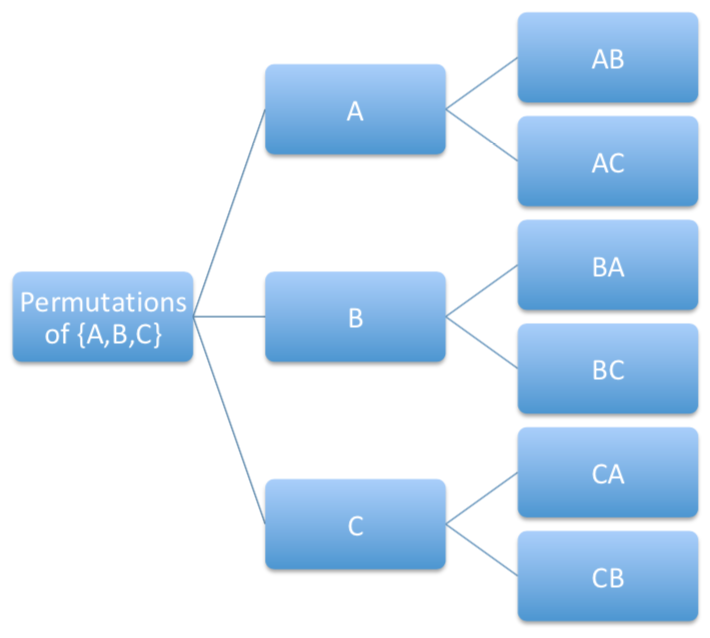
\includegraphics[width=\linewidth]{images/PermutationSmall.png}
\end{image}%
%
\par
Going one step further, what about ordering the letters in \textbraceleft{}A, B, C, D\textbraceright{}? You can start by picking one of the four letters, say A, and then arranging B, C, and D.  Then, start with B and arrange A, C, and D and so on.  This gives:%
\par
ABCD, ABDC, ACBD, ACDB, ADBC, ADCB%
\par
BACD, BADC, BCAD, BCAB, BDAC, BDCA%
\par
CBAD, CBDA, CABD, CADB, CDBA, CDAB%
\par
DBCA, DBAC, DCBA, DCAB, DABC, DACB%
\par
which is 24 different options or \(4! = 4 \cdot 3 \cdot 2 \cdot 1 = 24\).  This can be viewed using a tree structure where each decision creates a new branch. \begin{image}{0}{1}{0}%
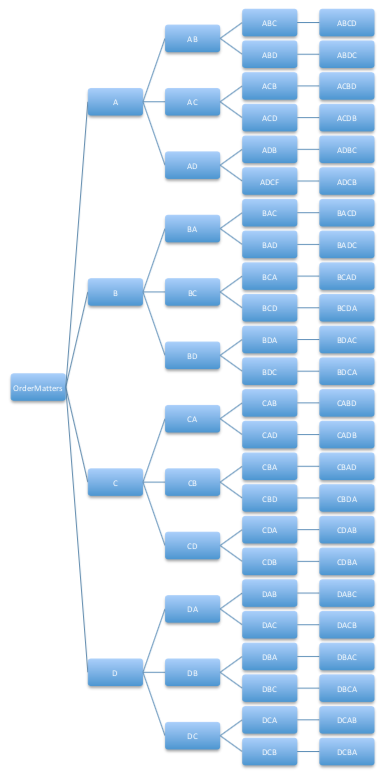
\includegraphics[width=\linewidth]{images/PermutationAllTree.png}
\end{image}%
%
\begin{theorem}{Permutations of a subset without replacement.}{}{x:theorem:PermutationWithoutReplacementDistinguishable}%
The number of ways to arrange r items from a set of n distinct items is%
\begin{equation*}
_nP_r = \frac{n!}{(n-r)!} 
\end{equation*}
This is sometimes denoted also as P(n,r) or \(P_r^n\).%
\end{theorem}
\begin{proof}{}{g:proof:idp103}
If \(r \gt n\) or \(r \lt 0 \) then this is not possible and so the result would be no permuatations. Otherwise, apply the multiplication principle r times noting that there are n choices for the first selection, n-1 choices for the second selection, and with n-r+1 choices for the rth selection. This gives%
\begin{align*}
_nP_r & = n(n-1) ... (n-r+1)\\
& = n(n-1) ... (n-r+1)\frac{(n-r)!}{(n-r)!}\\
& = \frac{n(n-1) ... (n-r+1)(n-r)!}{(n-r)!}\\
& = \frac{n!}{(n-r)!}\qedhere
\end{align*}
%
\end{proof}
Following the tree idea from above, continue for several steps but then stop once you have gone r steps in.  For example, it is easy to see that \(_5P_2 = 20\) using a tree. \begin{image}{0.25}{0.5}{0.25}%
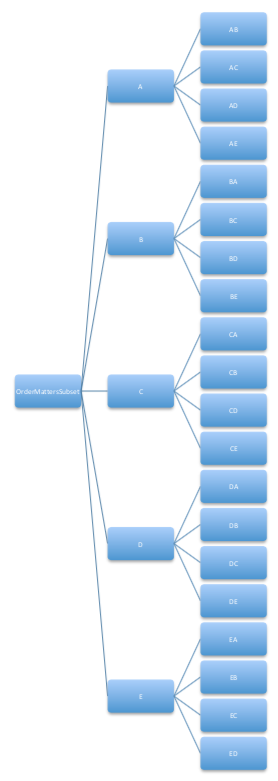
\includegraphics[width=\linewidth]{images/PermutationSubTree.png}
\end{image}%
%
\begin{inlineexercise}{WebWork - Permutations.}{g:exercise:idp104}%
In how many ways can 4 different novels, 2 different mathematics books, and 1 biology book be arranged on a bookshelf if%
\par
(a) the books can be arranged in any order?%
\par
Answer: \fillin{9.090909090909092}%
\par
(b) the mathematics books must be together and the novels must be together?%
\par
Answer: \fillin{9.090909090909092}%
\par
(c) the novels must be together but the other books can be arranged in any order?%
\par
Answer: \fillin{9.090909090909092}%
\par\smallskip%
\noindent\textbf{\blocktitlefont Answer 1}.\hypertarget{g:answer:idp105}{}\quad{}\(5040\)%
\par\smallskip%
\noindent\textbf{\blocktitlefont Answer 2}.\hypertarget{g:answer:idp106}{}\quad{}\(288\)%
\par\smallskip%
\noindent\textbf{\blocktitlefont Answer 3}.\hypertarget{g:answer:idp107}{}\quad{}\(576\)%
\end{inlineexercise}%
\begin{theorem}{Permutations of a subset with replacement.}{}{x:theorem:PermutationWithReplacementDistinguishable}%
The number of ways to obtain an arrangement of r choices from a group of size n is%
\begin{equation*}
n^r
\end{equation*}
%
\end{theorem}
\begin{proof}{}{g:proof:idp108}
Use the multiplication principle r times and see that for each choice all n objects in the universe remain available.  That is,%
\begin{equation*}
n \cdot n \cdot n ... n = n^r\qedhere
\end{equation*}
%
\end{proof}
\begin{theorem}{Permutations when not all items are distinguishable (Multinomial Coefficients).}{}{x:theorem:MultinomialCoefficients}%
If n items belong to s categories, \(n_1\) in first, \(n_2\) in second, ... , \(n_s\) in the last, the number of ways to pick all is%
\begin{equation*}
\frac{n!}{n_1! \cdot n_2! ... n_s!}
\end{equation*}
%
\end{theorem}
\begin{proof}{}{g:proof:idp109}
Enumerate all of the n data items individually with the \(n_1!\) identical values first and the remaining groups in like manner to get the enumerated list%
\begin{equation*}
\left \{ x_{1,1}, ..., x_{1,n_1}, x_{2,1}, ..., x_{2,n_2}, ... , x_{s,1}, ..., x_{s,n_s} \right \}
\end{equation*}
In this order, there are \(n_1!\) ways to arrange the first group, \(n_2!\) ways to arrange the second, etc. There are \(n_1! \times n_2! \times ... \times \n_s!\) ways to arrange all of the categories together with groups in this order but none of those group reorders does anything since those data values are all the same. Dividing out those from the \(n!\) original permutations of all items leaves one with the multinomial coefficient.%
\end{proof}
\begin{inlineexercise}{WebWork - More Permutations.}{g:exercise:idp110}%
How many anagrams can be created from the word 'metamorphosis' if the new words do not need to be meaningful? \fillin{15.9090909090909}%
\par\smallskip%
\noindent\textbf{\blocktitlefont Answer}.\hypertarget{g:answer:idp111}{}\quad{}\(7.78378\times 10^{8}\)%
\end{inlineexercise}%
\end{sectionptx}
%
%
\typeout{************************************************}
\typeout{Section 3.4 Combinations}
\typeout{************************************************}
%
\begin{sectionptx}{Combinations}{}{Combinations}{}{}{x:section:Combinations}
When counting various outcomes sometimes the order of things does not matter. If so, each unique unordered outcome is called a combination.%
\par
Once again, consider the permutations when selecting three letters from \textbraceleft{}A, B, C, D\textbraceright{}.%
\begin{enumerate}
\item{}%
\begin{itemize}[label=\textbullet]
\item{}A,B,C%
\item{}A,C,B%
\item{}B,A,C%
\item{}B,C,A%
\item{}C,A,B%
\item{}C,B,A%
\end{itemize}
%
\item{}%
\begin{itemize}[label=\textbullet]
\item{}A,B,D%
\item{}A,D,B%
\item{}B,A,D%
\item{}B,D,A%
\item{}D,A,B%
\item{}D,B,A%
\end{itemize}
%
\item{}%
\begin{itemize}[label=\textbullet]
\item{}A,C,D%
\item{}A,D,C%
\item{}C,A,D%
\item{}C,D,A%
\item{}D,A,C%
\item{}D,C,A%
\end{itemize}
%
\item{}%
\begin{itemize}[label=\textbullet]
\item{}B,C,D%
\item{}B,D,C%
\item{}C,B,D%
\item{}C,D,B%
\item{}D,B,C%
\item{}D,C,B%
\end{itemize}
%
\end{enumerate}
Notice how these 24 permutations fall into only four distinct categories if the order does not matter. Therefore, from a group of size four you can pick an unordered subset of size three in only 4 ways rather than the original 24.%
\par
In general, it would be nice to have a direct formula to determine the number of such combinations without having to explicitly list them all out.%
\begin{theorem}{Combinations of a subset without replacement.}{}{x:theorem:CombinationWithoutReplacementDistinguishable}%
The number of ways to arrange r items from a set of n distinct items is%
\begin{equation*}
_nC_r = \frac{n!}{r!(n-r)!} 
\end{equation*}
This is sometimes denoted C(n,r) or \(C_r^n\) or \({n \choose r}\).%
\end{theorem}
\begin{proof}{}{g:proof:idp112}
Consider creating a permutation of r objects from a set of size n by first picking an unordered subset of size r and then counting the number of ways to order that subset. Using our notation and the multiplication principle,%
\begin{equation*}
_nP_r = _nC_r \cdot r!
\end{equation*}
Dividing by \(r!\) gives the result.%
\end{proof}
\begin{theorem}{Combinations of a subset with replacement.}{}{x:theorem:CombinationWithReplacementDistinguishable}%
The number of ways to arrange r items from a set of n distinct items is%
\begin{equation*}
_{n+r-1}C_r = {{n+r-1} \choose r} = \frac{(r+n-1)!}{r!(n-1)!} 
\end{equation*}
%
\end{theorem}
\begin{proof}{}{g:proof:idp113}
Label each item in your group in some defined order. Since order doesn't matter, as you repeatedly sample r times with replacement you can always write down your outcomes sorted from low to high placement. Finally, separate like values by some symbol, say "\textbar{}", and consider each of the n distinct objects as indistinct \textasteriskcentered{}'s. There will be n-1 of these separators since there will be n to choose from. For example, if choosing r=6 times from the set \textbraceleft{}a, b, c, d\textbraceright{}, then the outcome b, b, a, d, a, b could be collected as a, a, b, b, b, d and written in our code as \textasteriskcentered{}\textasteriskcentered{}\textbar{}\textasteriskcentered{}\textasteriskcentered{}\textasteriskcentered{}\textbar{}\textbar{}\textasteriskcentered{} .  Notice that shuffling around the identical \textasteriskcentered{}'s would not change the code (and similarly for the identical \textbar{}'s) but swapping a \textasteriskcentered{} with a \textbar{} would be a different outcome. Therefore, we can consider this to be a \hyperref[x:theorem:MultinomialCoefficients]{multinomial coefficient~{\xreffont\ref{x:theorem:MultinomialCoefficients}}} and the number of ways to rearrange this code is%
\begin{equation*}
\frac{(r + n-1)!}{r!(n-1)!}.\qedhere
\end{equation*}
%
\end{proof}
\begin{inlineexercise}{WebWork - Combinations.}{g:exercise:idp114}%
A standard deck of cards consists of four suits (clubs, diamonds, hearts, and spades), with each suit containing 13 cards (ace, two through ten, jack, queen, and king) for a total of 52 cards in all.%
\par
How many 7-card hands will consist of exactly 2 hearts and 3 clubs?%
\par\smallskip%
\noindent\textbf{\blocktitlefont Answer}.\hypertarget{g:answer:idp115}{}\quad{}\(7.2501\times 10^{6}\)%
\par\medskip\noindent Notice that to determine the number of outcomes required you to use the combination forumula several times and then multiply the results using the multiplication principle.%
\par
\end{inlineexercise}%
\begin{inlineexercise}{WebWork - More Combinations.}{g:exercise:idp116}%
A school dance committee is to consist of 2 freshmen, 3 sophomores, 4 juniors, and 5 seniors. If 7 freshmen, 9 sophomores, 7 juniors, and 7 seniors are eligible to be on the committee, in how many ways can the committee be chosen?%
\par
Your answer is : \fillin{11.3636363636364}%
\par\smallskip%
\noindent\textbf{\blocktitlefont Answer}.\hypertarget{g:answer:idp117}{}\quad{}\(1296540\)%
\par\smallskip%
\noindent\textbf{\blocktitlefont Solution}.\hypertarget{g:solution:idp118}{}\quad{}\({7 \choose 2}\) ways to choose 2 freshmen for the committee, \({9 \choose 3}\) ways to choose 3 sophomores for the committee, \({7 \choose 4}\) ways to choose 4 juniors for the committee, and \({7 \choose 5}\) ways to choose 5 seniors for the committee. So by the generalized basic principle of counting, there are a total of%
\begin{equation*}
{7 \choose 2} \cdot {9 \choose 3} \cdot {7 \choose 4} \cdot {7 \choose 5}
= \frac{7 !}{2!5 !} \cdot \frac{9 !}{3! 6 !} \cdot \frac{7 !}{4! 3 !} \cdot \frac{7 !}{5! 2 !} = 1296540
\end{equation*}
\par\medskip\noindent Once again, you can see that using the formulas can be easy and also can be part of a bigger problem pasted together using the multiplication principle.%
\par
\end{inlineexercise}%
\begin{example}{Ipad Security.}{g:example:idp119}%
Revisiting your ipad's security, what happens if the order in which the digits are entered does not matter? If so, then you would be picking a combination of 4 digits without replacement from a group of 10 digits. Namely,%
\begin{align*}
\frac{10!}{4!6!} & = \frac{10 \times 9 \times 8 \times 7 \times 6!}{4 \times 3 \times 2 \times 1 \times 6!}\\
& = \frac{10 \times 9 \times 8 \times 7}{4 \times 3 \times 2 \times 1}\\
& = \frac{5040}{24}\\
& = 210.
\end{align*}
Notice that the total number of options is much smaller when order does not matter.%
\par
Note that if you were allowed to reuse the digits then the number of possible outcomes would be%
\begin{align*}
\frac{13!}{4!9!} & = \frac{13 \times 12 \times 11 \times 10}{4 \times 3 \times 2 \times 1} \\
& = 715
\end{align*}
which once again is more since numbers are allowed to repeat.%
\end{example}
\begin{definition}{Binomial Coefficients.}{x:definition:BinomialCoefficients}%
The value \(_nC_r\) is known as the binomial coefficient. It is denoted by \({n \choose r}\) and is read "n choose r".%
\end{definition}
Binomial coefficients have a number of interesting properties.  Many of these are very useful as well in probability calculations.  Several of these properties are collected below. In particular, these relationships verify that the binomial coefficients are the values found in Pascal's Triangle.%
\begin{sageinput}
@interact
def _(n = slider(1,15,1,5)):
    for row in range(n+1):
        binoms = sorted(binomial_coefficients(row).items())
        given_n = []
        for k in range(row+1):
            given_n.append(binoms[k][1])
        pretty_print('%s'%given_n)
\end{sageinput}
\begin{theorem}{Binomial Coefficient Formulas.}{}{x:theorem:BinomialCoefficientFormulas}%
For \(n \in \mathbb{N}\),%
\begin{enumerate}
\item{}\(\displaystyle \binom{n}{0} = 1\)%
\item{}\(\displaystyle \binom{n}{n} = 1\)%
\item{}\(\displaystyle \binom{n}{1} = n\)%
\item{}\(\displaystyle \binom{n}{n-1} = n\)%
\item{}\(\displaystyle \binom{n}{r} = \binom{n}{n-r}\)%
\item{}\(\displaystyle \binom{n+1}{r+1} = \binom{n}{r} + \binom{n}{r+1}\)%
\end{enumerate}
%
\end{theorem}
\begin{proof}{}{g:proof:idp120}
%
\begin{enumerate}
\item{}\(\displaystyle \binom{n}{0} = \frac{n!}{0!(n-0)!} = 1\)%
\item{}\(\displaystyle \binom{n}{n} = \frac{n!}{n!(n-n)!} = 1\)%
\item{}\(\displaystyle \binom{n}{1} = \frac{n!}{1!(n-1)!} = n\)%
\item{}\(\displaystyle \binom{n}{n-1} = \frac{n!}{(n-1)!(n-(n-1))!} = n\)%
\item{}\(\displaystyle \binom{n}{r} = \frac{n!}{r!(n-r)!} = \frac{n!}{(n-r)!(n-(n-r))!} = \binom{n}{n-r}\)%
\item{}%
\begin{align*}
\binom{n}{r} + \binom{n}{r+1} & = \frac{n!}{r!(n-r)!} + \frac{n!}{(r+1)!(n-(r+1))!}\\
& = (r+1) \frac{n!}{(r+1)!(n-r)!} \\ + (n-r) \frac{n!}{(r+1)!(n-r))!}\\
& = \frac{(r+1) n! + (n-r)n!}{(r+1)!(n-r)!}\\
& = \frac{(n+1) n!}{(r+1)!((n+1)-(r+1))!}\\
& = \binom{n+1}{r+1}
\end{align*}
%
\end{enumerate}
%
\end{proof}
\end{sectionptx}
%
%
\typeout{************************************************}
\typeout{Section 3.5 Summary}
\typeout{************************************************}
%
\begin{sectionptx}{Summary}{}{Summary}{}{}{x:section:CombinatoricsSummary}
\begin{introduction}{}%
Here are the important results from this chapter:%
\end{introduction}%
\hyperref[x:theorem:MultiplicationPrinciple]{Multiplication Principle~{\xreffont\ref{x:theorem:MultiplicationPrinciple}}}%
\par
\hyperref[x:definition:DefnFactorial]{Factorial~{\xreffont\ref{x:definition:DefnFactorial}}}%
\par
\hyperref[x:theorem:PermutationWithoutReplacementDistinguishable]{Permutations without replacement~{\xreffont\ref{x:theorem:PermutationWithoutReplacementDistinguishable}}}%
\par
\hyperref[x:theorem:PermutationWithReplacementDistinguishable]{Permutations with replacement~{\xreffont\ref{x:theorem:PermutationWithReplacementDistinguishable}}}%
\par
\hyperref[x:theorem:MultinomialCoefficients]{Multinomial Coefficients~{\xreffont\ref{x:theorem:MultinomialCoefficients}}}%
\par
\hyperref[x:theorem:CombinationWithoutReplacementDistinguishable]{Combinations without replacement~{\xreffont\ref{x:theorem:CombinationWithoutReplacementDistinguishable}}}%
\par
\hyperref[x:theorem:CombinationWithReplacementDistinguishable]{Combinations with replacement~{\xreffont\ref{x:theorem:CombinationWithReplacementDistinguishable}}}%
\par
\hyperref[x:definition:BinomialCoefficients]{Binomial Coefficients~{\xreffont\ref{x:definition:BinomialCoefficients}}}%
\end{sectionptx}
%
%
\typeout{************************************************}
\typeout{Section 3.6 Exercises}
\typeout{************************************************}
%
\begin{sectionptx}{Exercises}{}{Exercises}{}{}{x:section:CombinatoricsExercises}
Complete the online homework "Counting".%
\par
A standard deck of playing cards consists of 52 cards broken up into four "suits" known as Hearts, Spades, Diamonds, and Clubs. Each suit is broken up additionally into unique cards with "face values" from \textbraceleft{}2, 3, 4, 5, 6, 7, 8, 9, 10, Jack, Queen, King, Ace\textbraceright{} and generally in that order from low to high.%
\par
1.  Pick two cards without replacement one after the other from this deck and determine the following number of possible outcomes:%
\begin{itemize}[label=\textbullet]
\item{}The number of ways to get an Ace for both cards.%
\item{}The number of ways to get an Ace for only one of the two cards.%
\item{}The number of ways to get an Ace on the first draw and a Spade on the second draw.%
\end{itemize}
2.  Pick five cards without replacement one after the other from a newly shuffled full deck and determine the following number of possible outcomes:%
\begin{itemize}[label=\textbullet]
\item{}All cards have different faces%
\item{}"A pair". That is, two cards have the same face but the others are from three other faces.%
\item{}"Three of a kind".  That is, three cards have the same face but the others are from two other faces.%
\item{}"Two Pair". That is, two cards come from one face, two other cards come from a common face that is not the same as the first two cards, and the last card comes from some other face.%
\item{}"Full House". That is, three cards have the same face and the other two come from a common face that is not the same as the first three cards.%
\item{}"Four of a Kind". That is, four cards have the same face and the other card comes from some other face.%
\item{}"Flush". That is, the five cards for a sequence in order of adjacent faces in the original list and from the same suit.%
\item{}"Royal Flush". That is, a flush but only with the cards \textbraceleft{}Ace, King, Queen, Jack, 10\textbraceright{}.%
\end{itemize}
%
\par
Completely determine the number of possible passphrases for the National Treasure example started above. Present your answer in a report form.%
\end{sectionptx}
\end{chapterptx}
%
%
\typeout{************************************************}
\typeout{Chapter 4 Probability Theory}
\typeout{************************************************}
%
\begin{chapterptx}{Probability Theory}{}{Probability Theory}{}{}{x:chapter:ProbabilityGeneralities}
%
%
\typeout{************************************************}
\typeout{Section 4.1 Quantifying Uncertainty?}
\typeout{************************************************}
%
\begin{sectionptx}{Quantifying Uncertainty?}{}{Quantifying Uncertainty?}{}{}{x:section:ProbabilityGeneralitiesIntro}
Mathematics generally focuses on providing precise answers with absolute certainty. For example, solving an equation generates specific (and non-varying) solutions. Statistics on the other hand deals with providing precise answers to questions when there is uncertainty. It might seem impossible to provide such precise answers but the focus of this text is to show how that can be done so long as the questions are properly posed and the answers properly interpreted.%
\par
Indeed, people often make claims about being the biggest, best, most often recommended, etc. One sometimes even believes these claims based upon subjective metrics. In this chapter, we will start by looking at relative frequency and notice several properties regarding relative frequencies as the number of trials increases. We will use these examples to motivate a definition for probability and investigate the resulting consequences of that definition.%
\end{sectionptx}
%
%
\typeout{************************************************}
\typeout{Section 4.2 Relative Frequency}
\typeout{************************************************}
%
\begin{sectionptx}{Relative Frequency}{}{Relative Frequency}{}{}{x:section:RelativeFrequency}
When attempting to precisely measure uncertainty one often resorts to examples or experiments that model the theoretical question of interest. Before we investigate statistical experiments, we need to create some notation that we will utilize throughout the rest of this text.%
%
\begin{itemize}[label=\textbullet]
\item{}S = Universal Set or Sample Space Experiment or Outcome Space. This is the collection of all possiblilities.%
\item{}Random Experiment. A random experiment is a repeatable activity that has more than one possible outcome all of which can be specified in advance but can not be known in advance with certainty.%
\item{}Trial. Performing a Random Experiment one time and measuring the result.%
\item{}A = Event. A collection of outcomes.  Generally denoted by an upper case letter such as A, B, C, etc.%
\item{}Success\slash{}Failure. When recording the result of a trial, a success for event A occurs when the outcome lies in A. If not, then the trial was a failure. There is no qualitative meaning to this term.%
\item{}Mutually Exclusive Events. Two events that share no common outcomes. Also known as disjoint events.%
\item{}\textbar{}A\textbar{} = Frequency. In a sequence of n events, the frequency is the number of trials which resulted in a success for event A.%
\item{}\textbar{}A\textbar{} \slash{} n = Relative Frequency. A proportion of successes to total number of trials.%
\item{}Histogram. A bar chart representation of data where area corresponds to the value being described.%
\end{itemize}
To investigate these terms and to motivate our discussion of probability, consider flipping coins using the interactive cell below. Notice in this case, the sample space S = \textbackslash{}\textbraceleft{} Heads, Tails \textbackslash{}\textbraceright{} and the random experiment consists of flipping a fair coin one time. Each trial results in either a Head or a Tail. Since we are measuring both Heads and Tails then we will not worry about which is a success or failure. Further, on each flip the outcomes of Heads or Tails are mutually exclusive events. We count the frequencies and compute the relative frequencies for a varying number of trials selected by you as you move the slider bar. Results are displayed using a histogram.%
\begin{sageinput}
coin = ["Heads", "Tails"]
@interact
def _(num_rolls = slider([5..5000],label="Number of Flips")):
	rolls = [choice(coin) for roll in range(num_rolls)]
	show(rolls)   
	freq = [0,0]
	for outcome in rolls:
		if (outcome=='Tails'):
			freq[0] = freq[0]+1
		else:
			freq[1] = freq[1]+1
	print("The frequency of tails = %s"%str(freq[0])+" and heads = %s"%str(freq[1]))
	rel = [freq[0]/num_rolls,freq[1]/num_rolls]
	print("\nThe relative frequencies for Tails and Heads:"+str(rel))
	show(bar_chart(freq,axes=False,ymin=0,xmin=-1/2))     #  A histogram of the results
\end{sageinput}
Question 1: What do you notice as the number of flips increases?%
\par
Question 2: Why do you rarely (if ever) get exactly the same number of Heads and Tails? Would you not "expect" that to happen?%
\par
You should have noticed that as the number of flips increases, the relative frequency of Heads (and Tails) stabilized around 0.5. This makes sense intuitively since there are two options for each individual flip and 1\slash{}2 of those options are Heads while the other 1\slash{}2 is Tails.%
\par
Let's try again by doing a random experiment consisting of rolling a single die one time. Note that the sample space in this case will be the outcomes S = \textbraceleft{} 1, 2, 3, 4, 5, 6 \textbackslash{}.%
\begin{sageinput}
@interact
def _(num_rolls = slider([20..5000],label='Number of rolls'),Number_of_Sides = [4,6,8,12,20]):
	die = list((1..Number_of_Sides))
	rolls = [choice(die) for roll in range(num_rolls)]
	show(rolls)   

	freq = [rolls.count(outcome) for outcome in set(die)]  # count the numbers for each outcome
	print('The frequencies of each outcome is %s'%str(freq))

	print('The relative frequencies of each outcome:')
	rel_freq = [freq[outcome-1]/num_rolls for outcome in set(die)]  # make frequencies relative
	print(rel_freq)
	fs = []
	for f in rel_freq:
		fs.append(f.n(digits=4))
	print(fs)
	show(bar_chart(freq,axes=False,ymin=0,xmin=-1/2))
\end{sageinput}
Notice for a single die there are a larger number of options (for example 6 on a regular die) but once again the relative frequencies of each  outcome was close to 1\slash{}n (i.e. 1\slash{}6 for the regular die) as the number of rolls increased.%
\par
In general, this suggests a rule: if there are n outcomes and each one has the same chance of occurring on a given trial then on average on a large number of trials the relative frequency of that outcome is 1\slash{}n. In general, if a number of outcomes are "equally likely" then this is a good model for measuring the proportion of outcomes that would be expected to have any given outcome. However, it is not always true that outcomes are equally likely. Consider rolling two die and measuring their sum:%
\begin{sageinput}
@interact
def _(num_rolls = slider([20..5000],label='Number of rolls'),num_sides = slider(4,20,1,6,label='Number of sides')):
    die = list((1..num_sides))
    dice = list((2..num_sides*2))
    rolls = [(choice(die),choice(die)) for roll in range(num_rolls)]
    sums = [sum(rolls[roll]) for roll in range(num_rolls)]
    show(rolls)   

    freq = [sums.count(outcome) for outcome in set(dice)]  # count the numbers for each outcome
    print('The frequencies of each outcome is %s'%str(freq))
    
    print('The relative frequencies of each outcome:')
    rel_freq = [freq[outcome-2]/num_rolls for outcome in set(dice)]  # make frequencies relative
    print(rel_freq)
    show(bar_chart(freq,axes=False,ymin=0, xmin=-1))     #  A histogram of the results
    print("Relative Frequence of %s"%str(dice[0])+" is about %s"%str(rel_freq[0].n(digits=4)))
    print("Relative Frequence of %s"%str(dice[num_sides-1])+" is about %s"%str(rel_freq[num_sides-1].n(digits=4)))
\end{sageinput}
Question 1: What do you notice as the number of rolls increases?%
\par
Question 2: What do you expect for the relative frequencies and why are they not all exactly the same?%
\par
Notice, not only are the answers not the same but they are not even close. To understand why this is different from the examples before, consider the possible outcomes from each pair of die. Since we are measuring the sum of the dice then (for a pair of standard 6-sided dice) the possible sums are from 2 to 12. However, there is only one way to get a 2-{}-{}namely from a (1,1) pair-{}-{}while there are 6 ways to get a 7-{}-{}namely from the pairs (1,6), (2,5), (3,4), (4,3), (5,2), and (6,1). So it might make some sense that the likelihood of getting a 7 is 6 times larger than that of getting a 2. Check to see if that is the case with your experiment above.%
\par
Play with the following several times to investigate what you might expect to get when you repeatedly receive a "hand" of 5 standard playing cards. Can you imagine how you might possible enumerate the entire list of possible outcomes by hand? However, using this interactive cell, you can shuffle and deal 5-card hands over and over easily and then count the number of special poker outcomes.%
\begin{sageinput}
var('A C D H J K Q S') 

suits = [S, D, C, H] 
values = [2, 3, 4, 5, 6, 7, 8, 9, 10, J, Q, K, A] 

full_deck = [(value, suit) for suit in suits for value in values]
@interact
def _(num_hands=slider[50..5000]):                  # Set up the number of hands to create
    hands= []                    # Start with a blank list. 
    for i in range(num_hands):   # This loops the following operation num_hands times. 
        deck = copy(full_deck)   # start over
        shuffle(deck)
        hands.append([deck.pop() for card in range(5)])
    freq_values = []
    one_pair = 0
    two_pair = 0
    three_kind = 0
    full_house = 0
    four_kind = 0
    for i in range(num_hands):
        hand = hands[i]
        hand_values = [hand[k][0] for k in range(5)]
        freq_values = [hand_values.count(value) for value in set(values)]
        freq_values.sort(reverse=True)
        if freq_values[0]==4:
            four_kind=four_kind+1
        if freq_values[0]==3:
            if freq_values[1]==2:
                full_house=full_house+1
            if freq_values[1]==1:
                three_kind=three_kind+1
        if freq_values[0]==2:
            if freq_values[1]==2:
                two_pair=two_pair+1
            if freq_values[1]==1:
                one_pair=one_pair+1
    print("       One Pair frequency = %s"%str(one_pair)+" with relative frequency %s"%str(one_pair/num_hands))
    print("       Two Pair frequency = %s"%str(two_pair)+" with relative frequency %s"%str(two_pair/num_hands))
    print("Three of a Kind frequency = %s"%str(three_kind)+" with relative frequency %s"%str(three_kind/num_hands))
    print("     Full House frequency = %s"%str(full_house)+" with relative frequency %s"%str(full_house/num_hands))
    print(" Four of a Kind frequency = %s"%str(four_kind)+" with relative frequency %s"%str(four_kind/num_hands))
\end{sageinput}
Sometimes you will find it useful to keep a running total of the relative frequencies. Such a cumulative approach is often called a distribution function.%
\begin{definition}{Cumulative relative frequency.}{g:definition:idp121}%
For a collection of ordered events \(x_1 \lt x_2 \lt ... \lt x_s\) with corresponding frequencies \(f_1, f_2, ..., f_s\), the cumulative relative frequency is the function%
\begin{equation*}
F(x) = \sum_{x_k \le x} f_{x_k}
\end{equation*}
%
\end{definition}
Let's consider the cumulative relative frequency with the sum of dice example seen at the beginning of this chapter.%
\begin{sageinput}
@interact
def _(num_rolls = slider([20..5000],label='Number of rolls'),num_sides = slider(4,20,1,6,label='Number of sides')):
    die = list((1..num_sides))
    dice = list((2..num_sides*2))
    rolls = [(choice(die),choice(die)) for roll in range(num_rolls)]
    sums = [sum(rolls[roll]) for roll in range(num_rolls)]
    show(rolls)   

    freq = [sums.count(outcome) for outcome in set(dice)]  # count the numbers for each outcome
    n = len(freq)
    CF = freq
    for k in range(1,n):
        CF[k] = freq[k] + CF[k-1]
    
    print('The cumulative relative frequencies of each outcome:')
    Crel_freq = [CF[outcome-2]/num_rolls for outcome in set(dice)]  # make frequencies relative
    print(Crel_freq)        
    show(bar_chart(CF,axes=False,ymin=0, xmin= -1))     #  A histogram of the results
    print("Cumulative Relative Frequence of %s"%str(dice[0])+" is about %s"%str(Crel_freq[0].n(digits=4)))
    print("Cumulative Relative Frequence of %s"%str(dice[num_sides-1])+" is about %s"%str(Crel_freq[num_sides-1].n(digits=4)))
\end{sageinput}
\end{sectionptx}
%
%
\typeout{************************************************}
\typeout{Section 4.3 Definition of Probability}
\typeout{************************************************}
%
\begin{sectionptx}{Definition of Probability}{}{Definition of Probability}{}{}{x:section:ProbabilityBasics}
Relative frequency gives a way to measure the proportion of "successful" outcomes when doing an experimental approach. From the interactive applications above, it appears that the relative frequency does jump around as the experiment is repeated but that the amount of variation decreases as the number of experiments increases. This is known to be true in general and is known as the "Law of Large Numbers".%
\par
We would like to formalize what these relative frequencies are approaching and will call this theoretical limit the "probability" of the outcome. In doing so, we will do our best to model our definition so that it follow the behavior of relative frequency.%
\par
To generate a general definition for probability, we need to know what is is that we measuring. In general, we will be finding the probability of sets of possible outcomes...that is, a subset of the Sample Space S. Toward that end, it is important to briefly look at some properties of sets.%
\begin{definition}{Pairwise Disjoint Sets.}{x:definition:DefnMutuallyExclusive}%
\(\{ A_1, A_2, ... , A_n \}\) are pairwise disjoint provided \(A_k \cap A_j = \emptyset\) so long as \(k \ne j\). Disjoint sets as also often called mutually exclusive.%
\end{definition}
Play around with the interactive cell below by adding and removing items in each of the three sets. Find elements so that the intersection of all three sets is empty but at least one of the paired sets are not disjoint.  See if you can make all of the paired sets not disjoint but the intersection of all three disjoint. This is why we need to consider "pairwise" disjoint sets.%
\begin{sageinput}
def f(s, braces=True): 
    t = ', '.join(sorted(list(s)))
    if braces: return '{' + t + '}'
    return t
def g(s): return set(str(s).replace(',',' ').split())

@interact
def _(X='1,2,3', Y='2,a,3,4,apple', Z='a,b,10,apple'):
    S = [g(X), g(Y), g(Z)]
    X,Y,Z = S
    XY = X & Y
    XZ = X & Z
    YZ = Y & Z
    XYZ = XY & Z

    Txy = " - NOT disjoint "
    if Set(XY).is_empty():
        Txy = ' - disjoint '
    pretty_print(html("$X \\cap Y$ = %s"%f(XY)+"%s"%Txy))
    Txz = " - NOT disjoint "
    if Set(XZ).is_empty():
        Txz = ' - disjoint '
    pretty_print(html("$X \\cap Z$ = %s"%f(XZ)+"%s"%Txz))
    Tyz = " - NOT disjoint "
    if Set(YZ).is_empty():
        Tyz = ' - disjoint ' 
    pretty_print(html("$Y \\cap Z$ = %s"%f(YZ)+"%s"%Tyz))
    Txyz = " - NOT disjoint "
    if Set(XYZ).is_empty():
        Txyz = ' - disjoint ' 
    pretty_print(html("$X \\cap Y \\cap Z$ = %s"%f(XYZ)+"%s"%Txyz))
    centers = [(cos(n*2*pi/3), sin(n*2*pi/3)) for n in [0,1,2]]
    scale = 1.7
    clr = ['yellow', 'blue', 'green']
    G = Graphics()
    for i in range(len(S)):
        G += circle(centers[i], scale, rgbcolor=clr[i], 
             fill=True, alpha=0.3)
    for i in range(len(S)):
        G += circle(centers[i], scale, rgbcolor='black')

    # Plot what is in one but neither other
    for i in range(len(S)):
        Z = set(S[i])
        for j in range(1,len(S)):
            Z = Z.difference(S[(i+j)%3])
        G += text(f(Z,braces=False), (1.5*centers[i][0],1.7*centers[i][1]), rgbcolor='black')


    # Plot pairs of intersections
    for i in range(len(S)):
        Z = (set(S[i]) & S[(i+1)%3]) - set(XYZ)
        C = (1.3*cos(i*2*pi/3 + pi/3), 1.3*sin(i*2*pi/3 + pi/3))
        G += text(f(Z,braces=False), C, rgbcolor='black')

    # Plot intersection of all three
    G += text(f(XYZ,braces=False), (0,0), rgbcolor='black')

    # Show it
    G.show(aspect_ratio=1, axes=False)
\end{sageinput}
Consider how we might create a definition for the expectation of a given outcome. To do so, first consider a desired collection of outcomes A. If each outcome in A is chosen randomly then we might consider using a formula similar to relative frequency and set a measure of expectation to be \textbar{}A\textbar{}\slash{}\textbar{}S\textbar{}. For example, on a standard 6-sided die, the expectation of the outcome A=\textbraceleft{}2\textbraceright{} from the collection S = \textbraceleft{}1,2,3,4,5,6\textbraceright{} could be \textbar{}A\textbar{}\slash{}\textbar{}S\textbar{} = 1\slash{}6.%
\par
From our example where we take the sum of two die, the outcome A = \textbraceleft{} 4,5 \textbraceright{} from the collection S = \textbraceleft{}2,3,4,...,12\textbraceright{} would be%
\begin{gather*}
|A| = | \{ (1,3),(2,2),(3,1),(1,4),(2,3),(3,2),(4,1) \}| = 7\\
|S| = | \{ (1,1),...,(1,6),(2,1),...,(2,6),...,(6,1),...,(6,6) \}| = 36
\end{gather*}
and so the expected relative frequency would be \textbar{}A\textbar{}\slash{}\textbar{}S\textbar{} = 7\slash{}36. Compare this theoretical value with the sum of the two outcomes from your experiment above.%
\par
We are ready to now formally give a name to the theoretical measure of expectation for outcomes from an experiment. Taking our cue from our examples, let's make our definition agree with the following relative frequency properties:%
\begin{enumerate}
\item{}Relative frequency cannot be negative, since cardinality cannot be negative%
\item{}Relative frequencies for disjoint events should sum to one%
\item{}Relative frequencies for collections of disjoint outcomes should equal the sum of the individual relative frequencies%
\end{enumerate}
%
\par
which leads us to the following formal definition...%
\begin{definition}{Probability.}{x:definition:DefnProb}%
The probability P(A) of a given outcome A is a set function that satisfies:%
\par
%
\begin{enumerate}
\item{}(Nonnegativity) P(A) \(\ge 0\)%
\item{}(Totality) P(S) = 1%
\item{}(Subadditivity) If A \(\cap\) B = \(\emptyset\), then P(A \(\cup\) B) = P(A) + P(B). In general, if \textbraceleft{}\(A_k\)\textbraceright{} are pairwise disjoint then \(P( \cup_k A_k) = \sum_k P(A_k)\).%
\end{enumerate}
%
\end{definition}
\begin{inlineexercise}{WeBWorK - Using the definition.}{g:exercise:idp122}%
Suppose you select a letter at random from the word MISSISSIPPI.%
\par
The probability of selecting the letter M is \fillin{1.818181818181818}%
\par
The probability of selecting the letter S is \fillin{1.818181818181818}%
\par
The probability of selecting the letters P or I is \fillin{1.818181818181818}%
\par
The probability of not selecting the letter I is \fillin{1.818181818181818}%
\par\smallskip%
\noindent\textbf{\blocktitlefont Hint}.\hypertarget{g:hint:idp123}{}\quad{}Count the number of letters in the word.  When computing each probability, this is the number that goes on the bottom.%
\par\smallskip%
\noindent\textbf{\blocktitlefont Answer 1}.\hypertarget{g:answer:idp124}{}\quad{}\({\textstyle\frac{1}{11}}\)%
\par\smallskip%
\noindent\textbf{\blocktitlefont Answer 2}.\hypertarget{g:answer:idp125}{}\quad{}\({\textstyle\frac{4}{11}}\)%
\par\smallskip%
\noindent\textbf{\blocktitlefont Answer 3}.\hypertarget{g:answer:idp126}{}\quad{}\({\textstyle\frac{2}{11}}+{\textstyle\frac{4}{11}}\)%
\par\smallskip%
\noindent\textbf{\blocktitlefont Answer 4}.\hypertarget{g:answer:idp127}{}\quad{}\(1-{\textstyle\frac{4}{11}}\)%
\par\smallskip%
\noindent\textbf{\blocktitlefont Solution}.\hypertarget{g:solution:idp128}{}\quad{}The probability of 'M's is 1\slash{}11.%
\par
The probability of 'I's is 4\slash{}11.%
\par
The probability of 'S's is 4\slash{}11.%
\par
The probability of 'P's is 2\slash{}11.%
\par\medskip\noindent Notice when you are given complete information regarding the entire data set then determining probabilities for events can be relatively easy to compute.%
\par
\end{inlineexercise}%
Based upon this definition we can immediately establish a number of results.%
\begin{theorem}{Probability of Complements.}{}{x:theorem:ProbabilityComplements}%
For any event A,%
\begin{equation*}
P(A) + P(A^c) = 1
\end{equation*}
%
\end{theorem}
\begin{proof}{}{g:proof:idp129}
Let A be any event and note that%
\begin{equation*}
A \cap A^c = \emptyset.
\end{equation*}
But \(A \cup A^c = S\). So, by subadditivity%
\begin{equation*}
1 = P(S) = P(A \cup A^c) = P(A) + P(A^c)
\end{equation*}
as desired.%
\end{proof}
\begin{theorem}{}{}{x:theorem:ProbabilityEmptySet}%
%
\begin{equation*}
P(\emptyset) = 0
\end{equation*}
%
\end{theorem}
\begin{proof}{}{g:proof:idp130}
Note that \(\emptyset^c = S\). So, by the theorem above,%
\begin{equation*}
1 = P(S) + P(\emptyset) \Rightarrow 1 = 1 + P(\emptyset).
\end{equation*}
Cancelling the 1 on both sides gives \(P(\emptyset) = 0\).%
\end{proof}
\begin{theorem}{}{}{x:theorem:ProbabilityContainment}%
For events A and B with%
\begin{equation*}
A \subset B, P(A) \le P(B)\text{.}
\end{equation*}
\end{theorem}
\begin{proof}{}{g:proof:idp131}
Assume sets A and B satisfy \(A \subset B\). Then, notice that%
\begin{equation*}
A \cap (B-A) = \emptyset
\end{equation*}
and%
\begin{equation*}
B = A \cup (B-A).
\end{equation*}
Therefore, by subadditivity and nonnegativity%
\begin{gather*}
0 \le P(B-A)\\
P(A) \le P(A) + P(B-A) \\
P(A) \le P(B)\qedhere
\end{gather*}
%
\end{proof}
\begin{theorem}{}{}{x:theorem:ProbabilityLessThanOne}%
For any event A,%
\begin{equation*}
P(A) \le 1
\end{equation*}
\end{theorem}
\begin{proof}{}{g:proof:idp132}
Notice \(A \subset S\). By the theorem above \(P(A) \le P(S) = 1\)%
\end{proof}
\begin{theorem}{}{}{x:theorem:ProbabilityTwoUnions}%
For any sets A and B,%
\begin{equation*}
P(A \cup B) = P(A) + P(B) - P(A \cap B)
\end{equation*}
\end{theorem}
\begin{proof}{}{g:proof:idp133}
Notice that we can write \(A \cup B\) as the disjoint union%
\begin{equation*}
A \cup B = (A-B) \cup (A \cap B) \cup (B-A).
\end{equation*}
We can also write disjointly%
\begin{gather*}
A = (A-B) \cup (A \cap B)\\
B = (A \cap B) \cup (B-A)
\end{gather*}
Hence,%
\begin{align*}
P(A) & + P(B) - P(A \cap B) \\
& = [P(A-B) + P(A \cap B)] \\
& + [P(A \cap B) + P(B-A)] - P(A \cap B)\\
& = P(A-B) + P(A \cap B) + P(B-A)\\
& = P(A \cup B)\qedhere
\end{align*}
%
\end{proof}
This result can be extended to more that two sets using a property known as inclusion-exclusion. The following two theorems illustrate this property and are presented without proof.%
\begin{corollary}{}{}{x:corollary:ProbabilityThreeUnions}%
For any sets A, B and C,%
\begin{align*}
P(A \cup B \cup C) & = P(A) + P(B) + P(C)\\
& - P(A \cap B) - P(A \cap C) - P(B \cap C) \\
& + P(A \cap B \cap C)
\end{align*}
%
\end{corollary}
\begin{corollary}{}{}{x:corollary:ProbabilityFourUnions}%
For any sets A, B, C and D,%
\begin{align*}
P(A \cup B \cup C \cup D) & = P(A) + P(B) + P(C) + P(D)\\
& - P(A \cap B) - P(A \cap C) - P(A \cap D) \\
& - P(B \cap C) - P(B \cap D) - P(C \cap D)\\
& + P(A \cap B \cap C) + P(A \cap B \cap D) \\
& + P(A \cap C \cap D) + P(B \cap C \cap D)\\
& - P(A \cap B \cap C \cap D)
\end{align*}
%
\end{corollary}
Many times, you will be dealing with making selections from a sample space where each item in the space has an equal chance of being selected. This may happen (for example) when items in the sample space are of equal size or when selecting a card from a completely shuffled deck or when coins are flipped or when a normal fair die is rolled.%
\par
It is important to notice that not all outcomes are equally likely-{}-{}even in times when there are only two of them. Indeed, it is generally not an equally likely situation when picking the winner of a football game which pits, say, the New Orleans Saints professional football team with the New Orleans Home School Saints. Even though there are only two options the probability of the professional team winning in most years ought to be much greater than the chances that the high school will prevail.%
\par
When items are equally likely (sometimes also called "randomly selected") then each individual event has the same chance of being selected as any other. In this instance, determining the probability of a collection of outcomes is relatively simple.%
\begin{theorem}{Probability of Equally Likely Events.}{}{g:theorem:idp134}%
If outcomes in S are equally likely, then for \(A \subset S,\)%
\begin{equation*}
P(A) = \frac{|A|}{|S|}.
\end{equation*}
%
\end{theorem}
\begin{proof}{}{g:proof:idp135}
Enumerate S = \textbraceleft{}\(x_1, x_2, ..., x_{|S|}\)\textbraceright{} and note \(P( \{ x_k \} ) = c\) for some constant c since each item is equally likely. However, using each outcome as a disjoint event and the definition of probability,%
\begin{align*}
1 = P(S) & = P( \{ x_1 \} \cup \{x_2 \} \cup ... \cup \{x_{|S|} \} )\\
& = P(\{ x_1 \}) + P(\{ x_2 \} ) + ... + P(\{ x_{|S|} \} )\\
& = c + c + ... + c = {|S|} \times c
\end{align*}
and so \(c = \frac{1}{{|S|}}\). Therefore, \(P( \{ x_k \} ) = \frac{1}{|S|}\) .%
\par
Hence, with A = \textbraceleft{}\(a_1, a_2, ..., a_{|A|}\)\textbraceright{}, breaking up the disjoint probabilities as above gives%
\begin{align*}
P(A) & = P( \{ a_1 \} \cup \{ a_2 \} \cup ... \cup \{ a_{|A|} \} )\\
& = P(\{ a_1 \}) + P(\{ a_2 \} ) + ... + P(\{ a_{|A|} \} )\\
& = \frac{1}{{|S|}} + \frac{1}{{|S|}} + ... + \frac{1}{{|S|}}\\
& = \frac{|A|}{{|S|}}
\end{align*}
as desired.%
\end{proof}
\begin{sageinput}
var('A C D H J K Q S') 

def L(str):
    n = len(str)
    m = int(n/5)
    top = m+1
    if m == n/5:
        top = m
    for k in range(top):
        print(str[5*k:5*k+5])
        
suits = [S, D, C, H] 
values = [2, 3, 4, 5, 6, 7, 8, 9, 10, J, Q, K, A] 

deck = [(value, suit) for suit in suits for value in values]
full_deck = copy(deck)  # to save a copy of the original deck for later use.

# L(deck)
shuffle(deck)
# L(deck)
deck1 = copy(full_deck)
shuffle(deck1)

@interact
def _(auto_update=False):
    global deck1    
    shuffle(deck1)            
    if (Set(deck1).cardinality() < 5):
        print('Deck is too small...getting a new deck')
        deck1 = copy(full_deck)
    else:
        hand = [deck1.pop() for card in range(5)] 
        pretty_print("The cards dealt:")
        L(hand)
        pretty_print(" The remaining cards in the deck:")
        L(deck1)
        pretty_print(html("\n The number of remaining cards in the deck = %s"%str(Set(deck1).cardinality())))
\end{sageinput}
Let's see if you understand the relationship between frequency and relative frequency. In this exercise, presume "Probabiity" to be the expected fraction of outcomes you might logically expect.%
\begin{inlineexercise}{WebWork - Equally Likely.}{g:exercise:idp136}%
A fun size bag of M\(\\amp \)Ms has about 15 candies.  You open one of the bags and discover:%
\par
2 Blues, 2 Yellows, 5 Browns, 3 Reds and 3 Greens.%
\par
The probability of choosing a brown is \fillin{1.818181818181818}.%
\par
The odds in favor of choosing a yellow is \fillin{1.818181818181818}%
\par
The probability of choosing either a blue or a red is \fillin{1.818181818181818}%
\par
The odds against a green being chosen is \fillin{1.818181818181818}%
\par\smallskip%
\noindent\textbf{\blocktitlefont Hint}.\hypertarget{g:hint:idp137}{}\quad{}Odds in favor of an event = number of favorable outcomes \slash{} number of unfavorable outcomes.%
\par
Odds against an event = number of unfavorable outcomes \slash{} number of favorable outcomes.%
\par\smallskip%
\noindent\textbf{\blocktitlefont Answer 1}.\hypertarget{g:answer:idp138}{}\quad{}\(\frac{5}{15}\)%
\par\smallskip%
\noindent\textbf{\blocktitlefont Answer 2}.\hypertarget{g:answer:idp139}{}\quad{}\(\frac{2}{15-2}\)%
\par\smallskip%
\noindent\textbf{\blocktitlefont Answer 3}.\hypertarget{g:answer:idp140}{}\quad{}\(\frac{2+3}{15}\)%
\par\smallskip%
\noindent\textbf{\blocktitlefont Answer 4}.\hypertarget{g:answer:idp141}{}\quad{}\(\frac{15-3}{3}\)%
\par\medskip\noindent So, by counting actual "equally likely" outcomes these probabilities are easy to compute.%
\par
\end{inlineexercise}%
\begin{inlineexercise}{WebWork - Easy Probabilities.}{g:exercise:idp142}%
(a) \(\) Count the number of ways to arrange a sample of \(2\) elements from a population of \(11\) elements. NOTE: Order is not important.%
\par
answer: \fillin{4.545454545454546}%
\par
(b) \(\) If random sampling is to be employed, the probability that any particular sample will be selected is \fillin{4.545454545454546}%
\par\smallskip%
\noindent\textbf{\blocktitlefont Answer 1}.\hypertarget{g:answer:idp143}{}\quad{}\(55\)%
\par\smallskip%
\noindent\textbf{\blocktitlefont Answer 2}.\hypertarget{g:answer:idp144}{}\quad{}\(0.0181818181818182\)%
\par\medskip\noindent Notice how the probabilities look similar to relative frequencies. It's just the case that you are counting ALL of the individual simple possibilities that lead to a success.%
\par
\end{inlineexercise}%
\end{sectionptx}
%
%
\typeout{************************************************}
\typeout{Section 4.4 Exercises}
\typeout{************************************************}
%
\begin{sectionptx}{Exercises}{}{Exercises}{}{}{x:section:ProbabilityBasicsExercises}
\begin{inlineexercise}{Poker.}{g:exercise:idp145}%
Determine the probabilities associated with the various 5-card hands. That is%
\begin{enumerate}
\item{}P(one pair)%
\item{}P(two pair)%
\item{}P(three of a kind)%
\item{}P(full house)%
\item{}P(four of a kind%
\item{}P(straight)%
\item{}P(flush)%
\item{}P(royal flush)%
\end{enumerate}
%
\end{inlineexercise}%
\begin{inlineexercise}{Dice.}{g:exercise:idp146}%
Determine the 36 possible outcomes related to the rolling a pair of fair dice. Justify why each of these outcomes is equally likely. Determine the probabilities associated with each possible sum.%
\par\smallskip%
\noindent\textbf{\blocktitlefont Solution}.\hypertarget{g:solution:idp147}{}\quad{}Remember, when using equally likely outcomes \textbar{}A\textbar{}\slash{}\textbar{}S\textbar{} assumes that the items counted for A are also in the sample space S.  In this case, for example, to determine the Probability of getting a sum of (say) 4 includes the rolls (1,3), (2,2), and (3,1). These three "successes" from the 36 possible ordered pairs gives P(4) = 3\slash{}36.  Similarly, P(5) = \textbar{}dice rolls with a sum of 5\textbar{}\slash{}36 = \textbar{}(1,4), (2,3), (3,2), (4,1)\textbar{} \slash{} 36 = 4\slash{}36.%
 Continue in this manner to determine the other possibilities and then compare to the experimental sage cell seen earlier for the sum of two dice.%
\end{inlineexercise}%
\begin{inlineexercise}{Skew Dice.}{g:exercise:idp148}%
Suppose you have one die which only has three possible sides labeled 1, 2, or 3. Suppose a second die has twelve equally likely sides with labels 1,2,3,4,4,5,5,6,6,7,8,9.  Justify that the probabilities associate with each possible sum is the same as the probabilities when using two normal 6-sided dice.%
\par\smallskip%
\noindent\textbf{\blocktitlefont Solution}.\hypertarget{g:solution:idp149}{}\quad{}Consider the outcome space%
\begin{equation*}
S = {(1,1), (1,2), (1,3), (1,4), (1,4), (1,5), (1, 5), \\
(1,6), (1,6), (1,7), (1,8), (1,9), (2,1) ... (3,9)}
\end{equation*}
Then P(5) = \textbar{}(1,4), (1,4), (2,3), (3,2) \textbar{}\slash{}36 = 4\slash{}36. Compare this to the exercise with regular dice performed above.  Similarly, compute the remaining probabilities.%
\end{inlineexercise}%
\begin{inlineexercise}{Craps.}{g:exercise:idp150}%
Analyze the dice game known as "craps": Roll a pair of dice and consider the sum. If that sum is 7 or 11, the one who rolls wins and can roll again. If the sum is 2, 3, or 12 -{}-{} known as craps -{}-{} the one who rolls loses but keeps the dice. For any other outcome (called the "point"), the one who rolls continues hoping to roll the point value again before rolling a 7. If successful, then the roller wins and starts the game anew. If a 7 appears first, the roller loses and the next person gets to be the roller.%
\par
So, a win can be obtained in two ways: 7 or 11 on first roll or getting the point before the 7 thereafter. Therefore, determine the probability of a win and the probability of a loss.%
\par\smallskip%
\noindent\textbf{\blocktitlefont Solution}.\hypertarget{g:solution:idp151}{}\quad{}\href{http://mathworld.wolfram.com/Craps.html}{"craps"}.%
\end{inlineexercise}%
\end{sectionptx}
%
%
\typeout{************************************************}
\typeout{Section 4.5 Conditional Probability}
\typeout{************************************************}
%
\begin{sectionptx}{Conditional Probability}{}{Conditional Probability}{}{}{x:section:ConditionalProbability}
When finding the probability of an event, sometimes you may need to consider past history and how it might affect things. Indeed, you might think that when the local station forecasts rain then the probability of it actually raining should be greater than if they forecast fair skies. At least that is the hope. :)  In this section, you will develop a way to deal with the probability of some event that might change dependent upon the occurence or not of some other event.%
\par
Indeed, consider what happens when you keep on dealing a hand of five cards from a shuffled deck but without replacement.  Notice how the probability of the same thing (such as P(getting a Heart on the next card)) oscillates based upon what cards came out of the deck on previous hands.%
\begin{sageinput}
print("Conditional Events - successively deal 5 cards w/o replacement" )

var('Ace Clubs Diamonds Hearts Jack King Queen Spades') 

suits = [Spades, Diamonds, Clubs, Hearts] 
values = [2, 3, 4, 5, 6, 7, 8, 9, 10, Jack, Queen, King, Ace] 

deck = [(value, suit) for suit in suits for value in values]
full_deck = copy(deck)  # to save a copy of the original deck for later use.

deck1 = copy(full_deck)
history1=[]
@interact
def _(choice=['Hearts','Spades','Diamonds','Clubs','New Deck'],again=['Repeat Same Suit']):
    global deck1, history1
    shuffle(deck1)
    if choice=='Hearts':
        suit = Hearts
    elif choice=='Spades':
        suit = Spades
    elif choice=='Diamonds':
        suit = Diamonds
    elif choice=='Clubs':
        suit = Clubs
    else:
        deck1 = copy(full_deck)
        shuffle(deck1)
        history1=[]
    if (Set(deck1).cardinality()<5):
        print("Deck is too small...get a new deck")
    elif choice!='New Deck':
        hand = [deck1.pop() for card in range(5)] 
        print("Click on a desired suit above to deal out another 5 card hand.  The cards dealt:")
        print(hand)
        print("The remaining cards in the deck:")
        print(deck1)
        num = Set(deck1).cardinality()
        print("\nThe number of remaining cards in the deck = %s"%str(num))
        looking = []
        for card in deck1:
            if card[1]==suit:
                looking.append(card)
        prob = float(Set(looking).cardinality())/num
        history1.append(prob)
        
        print('So, the remaining probability of getting a card from '+choice+' from the remaining cards is %s'%str(prob))
    list_plot(history1).show(xmin=0,xmax=9,ymin=0,ymax=1,figsize=(5,2))
\end{sageinput}
Now, consider the case when you put the cards back in, reshuffle, and then get 5 new cards...%
\begin{sageinput}
print('Independent Events - Successively deal 5 cards but WITH replacement')

var('Ace Clubs Diamonds Hearts Jack King Queen Spades') 

suits = [Spades, Diamonds, Clubs, Hearts] 
values = [2, 3, 4, 5, 6, 7, 8, 9, 10, Jack, Queen, King, Ace] 

deck = [(value, suit) for suit in suits for value in values]
full_deck = copy(deck)  # to save a copy of the original deck for later use.
deck1 = copy(full_deck)

h2=[]
@interact
def _(choice=['Heart','Spade','Diamond','Club'],again=['Repeat Same Suit']):

    if choice=='Hearts':
        suit = Hearts
    elif choice=='Spades':
        suit = Spades
    elif choice=='Diamonds':
        suit = Diamonds
    else:
        suit = Clubs

    deck1 = copy(full_deck)
    shuffle(deck1) 
    hand = [deck1.pop() for card in range(5)] 
    print("The cards dealt:")
    print(hand)
    print("Replacing this hand and reshuffling gives the remaining cards in the deck:")
    deck1 = copy(full_deck)
    shuffle(deck1)
    print(deck1)
    
    num = Set(deck1).cardinality()
    print("\nThe number of remaining cards in the deck = %s"%str(num))
    looking = []
    for card in deck1:
        if card[1]==suit:
            looking.append(card)
    prob = float(Set(looking).cardinality())/num
    h2.append(prob)
    
    print('So, the remaining probability of getting a '+choice+' from the remaining cards is %s'%str(prob))
    list_plot(h2).show(xmin=0,xmax=15,ymin=0,ymax=1,figsize=(5,2))
    
    print('Independent Events - Successively deal 5 cards but WITH replacement')
\end{sageinput}
\begin{example}{Changing Sample Space - Balls.}{g:example:idp152}%
Consider a box with three balls: one Red, one White, and one Blue.  Using an equally likely assumption, the probability of randomly pulling out a Red ball should be 1\slash{}3.  That is P(Red) = 1\slash{}3.%
\par
However, suppose that for a first trial you pull out the White ball and set it aside. Attempting to pull out another ball leaves you with only two options and so the probability of randomly pulling out a Red ball is 1\slash{}2. Notice that the probability changed for the second trial dependent on the outcome of the first trial.%
\end{example}
\begin{example}{Changing Sample Space - Cards.}{g:example:idp153}%
Consider a deck of 52 standard playing cards and a success occurs when a Heart is selected from the deck. When extracting one card randomly, the probability	of that card being a Heart is P(Heart) = 13\slash{}52.%
\par
Now, assume that one card has already been extracted and set aside.  Next, prepare to extract another. If the first card drawn was a Heart, then there are only 12 Hearts left for the second draw. However, if the first card drawn was not a Heart, then there are 13 Hearts available for the second draw. To compute this probability correctly, one need to formulate the question so that subadditivity can be utilized.%
\par
Let \(H_1\) be the outcome Heart on 1st draw and \(H_2\) be the outcome Heart on 2nd draw. Then,%
\begin{align*}
P(\text{Heart on 2nd draw}) & = P( [ H_1 \cap H_2 ] \cup [ H_1^c \cap H_2 ] )\\
& = P( H_1 \cap H_2 ) + P( H_1^c \cap H_2 )\\
& = \frac{ | H_1 \cap H_2 |}{| P( \text{Number of ways to get two cards} | }\\
& + \frac{ | H_1^c \cap H_2 | }{ | \text{Number of ways to get two cards} | }\\
& = \frac{13}{52} \cdot \frac{12}{51} + \frac{39}{52} \cdot \frac{13}{51} = \frac{12}{4 \cdot 51} + \frac{3 \cdot 13}{4 \cdot 51}	
\end{align*}
%
\end{example}
\begin{definition}{Conditional Probability.}{x:definition:DefnConditionalProbability}%
For sets A and B,%
\begin{equation*}
P(B | A) = \frac{P(A \cap B)}{ P(A) },
\end{equation*}
provided \(P(A) \gt 0\).%
\end{definition}
You can read \(P(B|A)\) as "the probability of B given A".%
\begin{theorem}{}{}{g:theorem:idp154}%
\hyperref[x:definition:DefnConditionalProbability]{Conditional Probability~{\xreffont\ref{x:definition:DefnConditionalProbability}}} satisfies all of the requirements of regular probability.%
\end{theorem}
\begin{proof}{}{g:proof:idp155}
By definition, for any event probability must be nonnegative. Therefore%
\begin{equation*}
P(A \cap B) \ge 0.
\end{equation*}
So,%
\begin{equation*}
P(B | A) = \frac{\text{positive or zero}}{\text{positive}}\ge 0.
\end{equation*}
%
\par
Further,%
\begin{equation*}
P (S | A) = P(A \cap S)/P(A) = P(A)/P(A) = 1.
\end{equation*}
For the third part, we will only consider the case when there are two disjoint sets B and C.  Then,%
\begin{align*}
P(B \cup C | A) & = \frac{P(A \cap (B \cup C)}{P(A)} \\
& = \frac{P( (A \cap B) \cup (A \cap C) )}{P(A)}\\
& = \frac{P(A \cap B)}{P(A)} + \frac{P(A \cap C)}{P(A)}\\
& = P(B | A) + P(C | A).\qedhere
\end{align*}
%
\end{proof}
\begin{theorem}{Multiplication Rule.}{}{x:theorem:MultiplicationRule}%
For any sets A and B,%
\begin{equation*}
P(A \cap B) = P(A) P(B | A) = P(B) P(A | B)
\end{equation*}
%
\end{theorem}
\begin{proof}{}{g:proof:idp156}
If \(P(A)=0\) or \(P(B)=0\), then the result is trivial. Otherwise, unravel the definition of \hyperref[x:definition:DefnConditionalProbability]{conditional probability~{\xreffont\ref{x:definition:DefnConditionalProbability}}} by taking the denominator to the other side. Also note that you can write \(A \cap B = B \cap A\).%
\end{proof}
\begin{inlineexercise}{WebWork - Disjoint Pieces.}{g:exercise:idp157}%
A bag contains \(4\) red marbles and \(5\) white marbles.  Two marbles are drawn in succession without replacement.  Find the probabilities of the following events:%
\par
\alert{1.} The first marble drawn is red and the second is white.%
\par
Answer: \fillin{9.090909090909092}%
\par
\alert{2.} Both marbles drawn are red.%
\par
Answer: \fillin{9.090909090909092}%
\par\smallskip%
\noindent\textbf{\blocktitlefont Answer 1}.\hypertarget{g:answer:idp158}{}\quad{}\(\frac{4}{9}\frac{5}{2\cdot 4}\)%
\par\smallskip%
\noindent\textbf{\blocktitlefont Answer 2}.\hypertarget{g:answer:idp159}{}\quad{}\(\frac{4}{9}\frac{4-1}{2\cdot 4}\)%
\par\medskip\noindent See how you had to break the given question up into two disjoint pieces.%
\par
\end{inlineexercise}%
\end{sectionptx}
%
%
\typeout{************************************************}
\typeout{Section 4.6 Bayes' Theorem}
\typeout{************************************************}
%
\begin{sectionptx}{Bayes' Theorem}{}{Bayes' Theorem}{}{}{x:section:Bayes}
\hyperref[x:definition:DefnConditionalProbability]{Conditional probabilities~{\xreffont\ref{x:definition:DefnConditionalProbability}}} can be computed using the methods developed above if the appropriate information is available. Some times you will however have some information available, such as \(P(A | B)\) but need \(P(B | A)\). The ability to "play around with history" by switching what has been presumed to occur leads to an important result known as Bayes' Theorem.%
\begin{theorem}{Bayes' Theorem.}{}{x:theorem:BayesTheorem}%
Let \(S = \{ S_1, S_2, ... , S_m \}\) where the \(S_k\) are pairwise disjoint and \(S_1 \cup S_2 \cup ... \cup S_m = S\) (i.e. a partition of the space S).  Then for any \(A \subset S\)%
\begin{equation*}
P(S_j | A) = \frac{P(S_j)P(A | S_j)}{\sum_{k=1}^m P(S_k)P(A | S_k)}.
\end{equation*}
The conditional probability \(P(S_j | A)\) is called the posterior probability of \(S_k\).%
\end{theorem}
\begin{proof}{}{g:proof:idp160}
Notice, by the definition of \hyperref[x:definition:DefnConditionalProbability]{conditional probability~{\xreffont\ref{x:definition:DefnConditionalProbability}}} and the \hyperref[x:theorem:MultiplicationRule]{multiplication rule~{\xreffont\ref{x:theorem:MultiplicationRule}}}%
\begin{equation*}
P(S_j | A) = \frac{P(S_j \cap A)}{P(A)} = \frac{P(S_j)P( A | S_j)}{P(A)}.
\end{equation*}
But using the disjointness of the partition%
\begin{align*}
P(A) & = P( (A \cap S_1) \cup (A \cup S_2) \cup ... \cup (A \cup S_m) )\\
& = P(A \cap S_1) + P(A \cup S_2) + ... + P(A \cup S_m)\\
& = P(S_1 \cap A) + P(S_2 \cup A) + ... + P(S_m \cup A)\\
& = P(S_1) P(A | S_1) + P(S_2)P(A | S_2) + ... + P(S_m)P(A | S_m)\\
& = \sum_{k=1}^m P(S_k)P(A | S_k)
\end{align*}
Put these two expansions together to obtain the desired result.%
\end{proof}
To illustrate this result, from the web site \url{http://stattrek.com/probability/bayes-theorem.aspx} consider the following problem:%
\par
Marie is getting married tomorrow, at an outdoor ceremony in the desert. In recent years, it has rained only 5 days each year. Unfortunately, the weatherman has predicted rain for tomorrow. When it actually rains, the weatherman correctly forecasts rain 90\% of the time. When it doesn't rain, he incorrectly forecasts rain 10\% of the time. What is the probability that it will rain on the day of Marie's wedding?%
\par
Notice, all days can be classified into one of two disjoint options:%
\begin{itemize}[label=\textbullet]
\item{}Rainy, in which case we can deduce from the given info that P(Rain) = 5\slash{}365%
\item{}Not Rainy, and since this is the complement of above, P(Not Rain) = 360\slash{}365%
\end{itemize}
In the notation of \hyperref[x:theorem:BayesTheorem]{Bayes Theorem~{\xreffont\ref{x:theorem:BayesTheorem}}}, let A represent a forecast of Rain and note you have%
\begin{equation*}
P(\text{Rain}) = P(S_1) = \frac{5}{365}
\end{equation*}
and%
\begin{equation*}
P(\text{Not Rain}) = P(S_2) = \frac{360}{365}.
\end{equation*}
Further, you are given the conditional probabilities%
\begin{equation*}
P(\text{ Forecast Rain | Rain}) = P( A | S_1) = 0.9
\end{equation*}
%
\begin{equation*}
P(\text{ Forecast Rain | Not Rain}) = P( A | S_2) = 0.1
\end{equation*}
Notice that the question provided requests that you find the probability of Rain given that the weatherman has forecasted rain. What is given on the other hand is the reverse of that conditional probability. Using Bayes' Theorem allows you to turn this around...%
\begin{align*}
P(\text{Rain}) &  = P(S_1) P( A | S_1) + P(S_2) P(A | S_2)\\
& = \frac{5}{365} \cdot 0.9 + \frac{360}{365} \cdot 0.1
\end{align*}
Hence, putting these together gives%
\begin{align*}
P(\text{Rain | Forecast Rain}) & = \frac{\frac{5}{365} \cdot 0.9}{\frac{5}{365} \cdot 0.9 + \frac{360}{365} \cdot 0.1}\\
& = \frac{5 \cdot 0.9}{5 \cdot 0.9 + 360 \cdot 0.1}\\
& = \frac{45}{45+360} \approx 0.111
\end{align*}
So, normally there is only approximately a 1.369 percent chance of rain (5\slash{}365) on a given day but given that the weatherman has forecast rain, the chance of rain increases to a little more than 11 percent.%
\par
Here's a standard and yet surprising example:%
\par
Your neighbor has 2 children. You learn that he has a daughter Anna. What is the probability that Anna’s sibling is a sister? Your first reaction might be that it is obviously 1\slash{}2 since (ok, roughly) it is equally likely that the other sibling was born female or male. But is that accurate?%
\par
If you were to list all of the possible female\slash{}male outcomes when having two children, then the sample space is S = \textbraceleft{}FF, FM, MF, MM\textbraceright{} with FM meaning the first child is female and the second is male. Assuming again that girls and boys are equally likely to be born, these 4 outcomes have equal probability of \(1/4\).%
\par
The question asks is whether the neighbor has another daughter in the set Fem2 = \textbraceleft{}FF\textbraceright{} but since Anna is a girl then the possible outcomes now is only Fem = \textbraceleft{}FF, FM, MF\textbraceright{}.%
\par
So,%
\begin{align*}
P(Fem2|Fem) & = \frac{P(Fem2 \cap Fem)}{P(Fem)} \\
& = \frac{P(FF)}{P(FF or FM or MF)}\\
& = \frac{\frac{1}{4}}{\frac{3}{4}} = \frac{1}{3}
\end{align*}
%
\par
\hyperref[x:theorem:BayesTheorem]{Bayes' Theorem~{\xreffont\ref{x:theorem:BayesTheorem}}} also works well in analyzing "Let's Make A Deal" finale choice.%
\begin{inlineexercise}{WebWork - Bayes'.}{g:exercise:idp161}%
A biomedical research company produces \(46 \%\) of its insulin at a plant in Kansas City, and the remainder is produced at a plant in Jefferson City.  Quality control has shown that \(0.6 \%\) of the insulin produced at the plant in Kansas City is defective, while \(0.8 \%\) of the insulin produced at the plant in Jefferson City is defective.  What is the probability that a randomly chosen unit of insulin came from the plant in Jefferson City given that it is defective?%
\par
(\alert{Hint:} Draw a tree diagram first)%
\par\smallskip%
\noindent\textbf{\blocktitlefont Answer}.\hypertarget{g:answer:idp162}{}\quad{}\(0.610169\)%
\par\medskip\noindent You have to be careful to extract the conditional probabilities from the problem.%
\par
\end{inlineexercise}%
\begin{inlineexercise}{WebWork- Bigger Bayes'.}{g:exercise:idp163}%
Data from Office on Smoking and Health, Centers for Disease Control and Prevention, indicate that 42\% of adults who did not finish high school, 34\% of high school graduates, 26\% of adults who completed some college, and 13\% of college graduates smoke.  Suppose that one individual is selected at random and it is discovered that the individual smokes.  Use the probabilities in the following table to calculate the probability that the individual is a college graduate.%
\begin{sidebyside}{1}{0}{0}{0}%
\begin{sbspanel}{1}%
{\centering%
{\tabularfont%
\begin{tabular}{BlBlBlB}\hrulemedium
Education&Employed&Unemployed\tabularnewline\hrulemedium
Not a high school graduate&0.0975&0.0080\tabularnewline\hrulemedium
High school graduate&0.3108&0.0128\tabularnewline\hrulemedium
Some college, no degree&0.1785&0.0062\tabularnewline\hrulemedium
Associate Degree&0.0849&0.0023\tabularnewline\hrulemedium
Bachelor Degree&0.1959&0.0041\tabularnewline\hrulemedium
Advanced Degree&0.0975&0.0015\tabularnewline\hrulemedium
\end{tabular}
}%
\par}
\end{sbspanel}%
\end{sidebyside}%
\par
Probability =  \fillin{6.818181818181818}%
\par
Hints: This problem has all the information you need, but not in the typical ready-to-use form.  The table above can tell you the proportion of people with various levels of education in the population. Keep in mind that any degree (Associate, Bachelor, or Advanced) counts as graduating from college.%
\par\smallskip%
\noindent\textbf{\blocktitlefont Answer}.\hypertarget{g:answer:idp164}{}\quad{}\(0.198786832540129\)%
\par\medskip\noindent Notice that having the data expressed in tabular form sometimes makes it easier to deal with.%
\par
\end{inlineexercise}%
The interactive cell below can be used to easily compute all of the conditional probabilities associated with \hyperref[x:theorem:BayesTheorem]{Bayes' Theorem~{\xreffont\ref{x:theorem:BayesTheorem}}}. Notice how the relative size of the pie-shaped partition changes when you presume that an event in the space has already occurred.%
\begin{sageinput}
#  This function is used to convert an input string into separate entries
def g(s): return str(s).replace(',',' ').replace('(',' ').replace(')',' ').split()

@interact
def _(Partition_Probabilities=input_box('0.35,0.25,0.40',label="$$ P(S_1),P(S_2),... $$"),
        Conditional_Probabilities=input_box('0.02,0.01,0.03',label='$$ P(A|S_1),P(A|S_2),... $$'),
        print_numbers=checkbox(True,label='Numerical Results on Graphs?'),
        auto_update=False):
            
    Partition_Probabilities = g(Partition_Probabilities)
    Conditional_Probabilities = g(Conditional_Probabilities)
    n = len(Partition_Probabilities)
    n0 = len(Conditional_Probabilities)
    
    # below needs to be n not equal to n0 but mathbook xml will not let me get the other
    if (n > n0):
        pretty_print("You must have the same number of partition probabilities and conditional probabilities.")
        
    else:                               # input data streams now are the same size!
        colors = rainbow(n)
        accum = float(0)                # to test whether partition probs sum to one
        ends = [0]                      # where the graphed partition sectors change in pie chart 
        mid = []                        # middle of each pie chart sector used for placement of text
        p_Sk_given_A = []               # P( S_k | A )
        pA = 0                          # P(A)
        PP=[]                           # array to hold the numerical Partition Probabilities 
        CP=[]                           # array to hold the numerical Conditional Probabilities     
        for k in range(n):
            PP.append(float(Partition_Probabilities[k]))
            CP.append(float(Conditional_Probabilities[k]))    
            p_Sk_given_A.append(PP[k]*CP[k] )
            pA += p_Sk_given_A[k]
            accum = accum + PP[k]
            ends.append(accum)
            mid.append((ends[k]+accum)/2)
#
#  Marching along from 0 to 1, saving angles for each partition sector boundary.
#  Later, we will multiple these by 2*pi to get actual sector boundary angles.
#
        if abs(accum-float(1))>0.0000001:     #  Due to roundoff issues, this should be close enough.                     
            pretty_print("Sum of probabilities should equal 1.")
        
        else:                           # probability data is sensible
 
#        
#  Draw the Venn diagram by drawing sectors from the angles determined above
#  First, create a circle of radius 1 to illustrate the the sample space S
#  Then draw each sector with varying colors and print out their names on the edge
#
            G = circle((0,0), 1, rgbcolor='black',fill=False, alpha=0.4,aspect_ratio=True,axes=False,thickness=5)
            for k in range(n):
                G += disk((0,0), 1, (ends[k]*2*pi, ends[k+1]*2*pi), color=colors[mod(k,10)],alpha = 0.2)
                G += text('$S_'+str(k+1)+'$',(1.1*cos(mid[k]*2*pi), 1.1*sin(mid[k]*2*pi)), rgbcolor='black')
                
            G += circle((0,0), 0.6, facecolor='yellow', fill = True, alpha = 0.1, thickness=5,edgecolor='black') 
    
#  Print the probabilities corresponding to each particular region as a list and on the graphs
            if print_numbers:               

                html("$P(A) = %s$"%(str(pA),))
                for k in range(n):
                    html("$P(S_{%s} | A)$"%(str(k+1))+"$ = %s$"%str(p_Sk_given_A[k]/pA))
                                        
                    G += text(str(p_Sk_given_A[k]),(0.4*cos(mid[k]*2*pi), 0.4*sin(mid[k]*2*pi)), rgbcolor='black')
                    G += text(str(PP[k] - p_Sk_given_A[k]),(0.8*cos(mid[k]*2*pi), 0.8*sin(mid[k]*2*pi)), rgbcolor='black')
        
#  This is essentially a repeat of some of the above code but focused only on creating the smaller inner circle dealing
#  with the set A so that the sectors now correspond in area to the Bayes Theorem probabilities


            accum = float(0)                        
            ends = [0]                     # where the graphed partition sectors change in pie chart 
            mid = []                       # middle of each pie chart sector used for placement of text
            for k in range(n): 
                accum += float(p_Sk_given_A[k]/pA) 
                ends.append(accum)
                mid.append((ends[k]+accum)/2)
            H = circle((0,0), 1, rgbcolor='black',fill=False, alpha=0,aspect_ratio=True,axes=False,thickness=0)
            H += circle((0,0), 0.6, facecolor='yellow',fill=True, alpha=0.1,aspect_ratio=True,axes=False,thickness=5,edgecolor='black')
            
            for k in range(n):
                H += disk((0,0), 0.6, (ends[k]*2*pi, ends[k+1]*2*pi), color=colors[mod(k,10)],alpha = 0.2)
                H += text('$S_'+str(k+1)+'|A$',(0.7*cos(mid[k]*2*pi), 0.7*sin(mid[k]*2*pi)), rgbcolor='black')
                    
        #  Now, print out the bayesian probabilities using the smaller set A only
    
            if print_numbers:
                for k in range(n):
                    H += text(str( N(p_Sk_given_A[k]/pA,digits=4) ),(0.4*cos(mid[k]*2*pi), 0.4*sin(mid[k]*2*pi)), rgbcolor='black')
                    
            G.show(title='Venn diagram of partition with A in middle')
            print
            H.show(title='Venn diagram presuming A has occured')
\end{sageinput}
You can actually also use \hyperref[x:theorem:BayesTheorem]{Bayes' Theorem~{\xreffont\ref{x:theorem:BayesTheorem}}} to answer a easy question!  Indeed, suppose that you draw one card from a shuffled and standard 52 card deck.  Given that you know the card is an Ace, what is the probability that it is also a Heart.%
\par
Using the Bayes' approach, let's break up the world into Hearts (H) and non-Hearts (N).  Easily,%
\begin{equation*}
P(A|H) = 1/13
\end{equation*}
%
\begin{equation*}
P(A|N) = 3/39
\end{equation*}
and so by Bayes'%
\begin{equation*}
P(H|A) = \frac{P(H) P(A|H)}{P(H) P(A|H) + P(N) P(A|N)} 
= \frac{\frac{13}{52} \cdot \frac{1}{13}}{\frac{13}{52} \cdot \frac{1}{13} + \frac{39}{52} \cdot \frac{3}{39}} = \frac{1}{4}
\end{equation*}
as expected!%
\begin{inlineexercise}{Insured vs Accident.}{g:exercise:idp165}%
Your automobile insurance company uses past history to determine how to set rates by measuring the number of accidents caused by clients in various age ranges. The following table summarizes the proportion of those insured and the corresponding probabilities by age range: \begin{tableptx}{\textbf{Age vs Accident Likelihood}}{g:table:idp166}{}%
\centering
{\tabularfont%
\begin{tabular}{rrr}
\multicolumn{1}{rB}{Age}&\multicolumn{1}{rB}{Proportion of Insured}&Probability of Accident\tabularnewline\hrulemedium
\multicolumn{1}{rB}{16-20}&\multicolumn{1}{rB}{0.05}&0.08\tabularnewline[0pt]
\multicolumn{1}{rB}{21-25}&\multicolumn{1}{rB}{0.06}&0.07\tabularnewline[0pt]
\multicolumn{1}{rB}{26-55}&\multicolumn{1}{rB}{0.49}&0.02\tabularnewline[0pt]
\multicolumn{1}{rB}{55-65}&\multicolumn{1}{rB}{0.25}&0.03\tabularnewline[0pt]
\multicolumn{1}{rB}{over 65}&\multicolumn{1}{rB}{0.15}&0.04
\end{tabular}
}%
\end{tableptx}%
 One of your family friends insured by this company has an accident.%
\begin{enumerate}
\item{}Determine the conditional probability that the driver was in the 16-20 age range.%
\item{}Compare this to the probability that the driver was in the 18-20 age range. Discuss the difference.%
\item{}Determine how much more the company should charge for someone in the 16-20 age range compared to someone in the 26-55 age range.%
\end{enumerate}
%
\par\smallskip%
\noindent\textbf{\blocktitlefont Solution}.\hypertarget{g:solution:idp167}{}\quad{}Plug the middle column into the first input box and the right column into the second input box of the Bayes Sage Cell.%
\end{inlineexercise}%
\begin{inlineexercise}{Spinal bifida odds.}{g:exercise:idp168}%
Congratulations...your family is having a baby! As part of the prenatal care, some testing is part of the normal procedure including one for spinal bifida (which is a condition in which part of the spinal cord may be exposed.) Indeed, measurement of maternal serum AFP values is a standard tool used in obstetrical care to identify pregnancies that may have an increased risk for this disorder. You want to make plans for the new child's care and want to know how serious to take the test results. However, some times the test indicates that the child has the disorder when in actuality it does not (a false positive) and likewise may indicate that the child does not have the disorder when in fact it does (a false negative.)%
\par
The combined accuracy rate for the screen to detect the chromosomal abnormalities mentioned above is approximately 85\% with a false positive rate of 5\%. This means that (from \href{http://americanpregnancy.org/prenatal-testing/first-trimester-screen/}{americanpregnancy.org})%
\begin{itemize}[label=\textbullet]
\item{}Approximately 85 out of every 100 babies affected by the abnormalities addressed by the screen will be identified. (Positive Positive)%
\item{}Approximately 5\% of all normal pregnancies will receive a positive result or an abnormal level. (False Positive)%
\end{itemize}
%
\begin{enumerate}
\item{}Given that your test came back negative, determine the likelihood that the child will actually have spinal bifida.%
\item{}Given that your test came back negative, determine the likelihood that the child will not have spina bifida%
\item{}Given that a positive test means you have a 1\slash{}100 to 1\slash{}300 chance of experiencing one of the abnormalities, determine the likelihood of spinal bifida in a randomly selected child.%
\end{enumerate}
You can get some help checking your arithmetic using the Bayes' Sage interact.%
\end{inlineexercise}%
\end{sectionptx}
%
%
\typeout{************************************************}
\typeout{Section 4.7 Independence}
\typeout{************************************************}
%
\begin{sectionptx}{Independence}{}{Independence}{}{}{x:section:Independence}
You have seen when repeatedly sampling without replacement leads to a change the the likelihood of some event in successive trials. Indeed, this is what conditional probabilities above illustrate. However, when sampling with replacement you may find a different situation arises. Indeed, you easily notice that when flipping a coin, P(Heads) = 1\slash{}2 regardless of the outcome of any previous flip.  In situations such as this where the probability of an event is not affected by the occurrence (or lack of occurrence) of some other event determining the probability of compound events can be greatly simplified.%
\begin{definition}{Independent Events.}{x:definition:DefnIndependentEvents}%
Events A and B are independent provided%
\begin{equation*}
P(A \cap B) = P(A) P(B)
\end{equation*}
%
\end{definition}
\begin{corollary}{Independence and Conditional Probability.}{}{g:corollary:idp169}%
Given \hyperref[x:definition:DefnIndependentEvents]{independent events~{\xreffont\ref{x:definition:DefnIndependentEvents}}} A and B,%
\begin{equation*}
P(B | A) = P(B)
\end{equation*}
and%
\begin{equation*}
P(A | B) = P(A).
\end{equation*}
%
\end{corollary}
\begin{proof}{}{g:proof:idp170}
By the multiplication rule and the definition of independence, for any events A and B%
\begin{equation*}
P(A) \cdot P(B) = P(A \cap B) = P(A) \cdot P(B | A) .
\end{equation*}
Therefore, if P(A) is non-zero, canceling yields the first result. Switching around notation provides the second.%
\end{proof}
\begin{inlineexercise}{WebWork - Independence.}{g:exercise:idp171}%
For two events \(A\) and \(B\), \(P(A) = 0.7\) and \(P(B) = 0.2\).%
\par
(a)\(\) If \(A\) and \(B\) are independent, then%
\par
\(P(A \cap B)\) \(=\) \fillin{4.545454545454546}%
\par
\(P(A \cup B)\) \(=\) \fillin{4.545454545454546}%
\par
\(P(A|B)\) \(=\) \fillin{4.545454545454546}%
\par
(b)\(\) If \(A\) and \(B\) are dependent and \(P(A|B) = 0.2\), then%
\par
\(P(B|A)\) \(=\) \fillin{4.545454545454546}%
\par
\(P(A \cap B)\) \(=\) \fillin{4.545454545454546}%
\par\smallskip%
\noindent\textbf{\blocktitlefont Answer 1}.\hypertarget{g:answer:idp172}{}\quad{}\(0.14\)%
\par\smallskip%
\noindent\textbf{\blocktitlefont Answer 2}.\hypertarget{g:answer:idp173}{}\quad{}\(0.76\)%
\par\smallskip%
\noindent\textbf{\blocktitlefont Answer 3}.\hypertarget{g:answer:idp174}{}\quad{}\(0.7\)%
\par\smallskip%
\noindent\textbf{\blocktitlefont Answer 4}.\hypertarget{g:answer:idp175}{}\quad{}\(0.0571428571428572\)%
\par\smallskip%
\noindent\textbf{\blocktitlefont Answer 5}.\hypertarget{g:answer:idp176}{}\quad{}\(0.04\)%
\par\medskip\noindent Basically you just multiply individual probabilities together.  Independence is often assumed since it makes computations easier. That said, you should remember to consider each time whether independence should or should not be assumed.%
\par
\end{inlineexercise}%
\begin{corollary}{Independence and Mutual Exclusivity.}{}{x:corollary:IndependenceVsDisjointness}%
If events A and B are both \hyperref[x:definition:DefnIndependentEvents]{independent~{\xreffont\ref{x:definition:DefnIndependentEvents}}} and \hyperref[x:definition:DefnMutuallyExclusive]{mutually exclusive~{\xreffont\ref{x:definition:DefnMutuallyExclusive}}}, then at least one of them has zero probability.%
\end{corollary}
\begin{proof}{}{g:proof:idp177}
By independence, \(P(A \cap B) = P(A) \cdot P(B)\). However, by mutually exclusivity, \(A \cap B = \emptyset \Rightarrow P(A \cap B) = 0\) gives%
\begin{equation*}
P(A) \cdot P(B) = 0.
\end{equation*}
Hence, one or the other (or both) must be zero.%
\end{proof}
\begin{corollary}{Successive Independent Events.}{}{g:corollary:idp178}%
Given a sequence of mutually independent events \(A_1, A_2, A_3, ...\),%
\begin{equation*}
P(\cap_{k \in R} A_k) = \prod_{k \in R} P(A_k)
\end{equation*}
%
\end{corollary}
\end{sectionptx}
%
%
\typeout{************************************************}
\typeout{Section 4.8 Summary}
\typeout{************************************************}
%
\begin{sectionptx}{Summary}{}{Summary}{}{}{x:section:ProbabilityGeneralitiesSummary}
TBA%
\end{sectionptx}
%
%
\typeout{************************************************}
\typeout{Section 4.9 More Exercises}
\typeout{************************************************}
%
\begin{sectionptx}{More Exercises}{}{More Exercises}{}{}{x:section:ProbabilityGeneralitiesExercises}
\begin{inlineexercise}{Conditional Basic computation.}{g:exercise:idp179}%
Given \(P(A) = 0.43, P(B) = 0.72,\) and \(P(A \cap B) = 0.29\), determine%
\begin{enumerate}
\item{}\(\displaystyle P(A \cup B)\)%
\item{}\(\displaystyle P(B | A)\)%
\item{}\(\displaystyle P(A | B)\)%
\item{}\(\displaystyle P(A^c \cap B^c)\)%
\end{enumerate}
%
\par\smallskip%
\noindent\textbf{\blocktitlefont Solution}.\hypertarget{g:solution:idp180}{}\quad{}Use the Theorems and Definitions provided to complete the first three.  For the fourth part, it might be useful to use DeMorgan's Laws from set theory to rewrite \(A^c \cap B^c = (A \cup B)^c\) and then use a theorem.%
\end{inlineexercise}%
\begin{inlineexercise}{Gender vs University Major.}{g:exercise:idp181}%
The table below classifies students at your university according to gender and according to major. \begin{tableptx}{\textbf{Gender vs Major}}{g:table:idp182}{}%
\centering
{\tabularfont%
\begin{tabular}{rrrr}
\multicolumn{1}{rB}{Enrollment}&Male&\multicolumn{1}{rB}{Female}&Totals\tabularnewline\hrulemedium
\multicolumn{1}{rB}{STEM}&420&\multicolumn{1}{rB}{510}&930\tabularnewline[0pt]
\multicolumn{1}{rB}{Business}&320&\multicolumn{1}{rB}{270}&590\tabularnewline[0pt]
\multicolumn{1}{rB}{Other}&610&\multicolumn{1}{rB}{710}&1320\tabularnewline\hrulemedium
\multicolumn{1}{rB}{Totals}&1350&\multicolumn{1}{rB}{1490}&2840
\end{tabular}
}%
\end{tableptx}%
 Determine the following:%
\begin{enumerate}
\item{}\(\displaystyle P( \text{STEM major} )\)%
\item{}\(\displaystyle P( \text{STEM | Female} )\)%
\item{}\(\displaystyle P( \text{Female | STEM} )\)%
\item{}\(\displaystyle P( \text{Female | Not STEM} )\)%
\end{enumerate}
%
\end{inlineexercise}%
\begin{inlineexercise}{Mean Tough Teacher.}{g:exercise:idp183}%
You are in a probability and statistics class with a teacher who has predetermined that only one student can make an A for the course. To be "fair", he places a number of slips of paper in a bowl equal to the number of students in the course with one of the slips having an A designation. Students in the course each can pick once randomly from the bowl and without replacement to see if they can get the lucky slip.  Determine the following:%
\begin{enumerate}
\item{}If there are 15 students in your course, determine the probabilities of getting an A in the course if you pick first and if you pick last.%
\item{}Since the teacher likes you the most, she will give you the option of deciding whether to pick at any position. If so, determine the position that would give you the best likelihood of getting the A slop.%
\item{}Suppose again that the teacher was feeling more generous and decided instead to allow for two A's. Determine how that changes your likelihood of winning and on what position you would like to choose.%
\item{}Continue as above except that only one slip does not have an A on it.%
\item{}Discuss how your choice is affected by the number of students in the course or the number of A slips included.%
\end{enumerate}
%
\par\smallskip%
\noindent\textbf{\blocktitlefont Solution}.\hypertarget{g:solution:idp184}{}\quad{}Using the normal equally-likely definition, \(P(\text{first}) = \frac{1}{15}\).%
\par
To get the A on the last pick requires that all of the previous picks to be something else. You don't get the opportunity to pick the A if it has already been selected. So, if L stands for losing (not getting the A), then%
\begin{align*}
P(\text{last}) & = P(\text{LLLLLLLLLLLLLLA}) \\
& = \frac{14 \cdot 13 \cdot 12 \cdot 11 \cdot 10 \cdot 9  \cdot 8  \cdot 7  \cdot 6  \cdot 5  \cdot 4  \cdot 3 \cdot 2  \cdot 1}{15 \cdot 14 \cdot 13 \cdot 12 \cdot 11 \cdot 10 \cdot 9 \cdot 8 \cdot 7 \cdot 6 \cdot 5 \cdot 4 \cdot 3 \cdot 2} = \frac{1}{15}.
\end{align*}
Therefore, it is the same probability of getting the A whether you pick first or last.  In general, to win on the kth pick gives%
\begin{align*}
P(\text{kth}) & = P(\text{LL...LA})\\
& = \frac{14 \cdot 13 \cdot ... \cdot (15-k) \cdot 1}{15 \cdot 14 ... \cdot (16-k) \cdot (15-k)} = \frac{1}{15}
\end{align*}
Hence, it is the same probability regardless of when you get to pick.%
\par
If there are two A's possible, then the options for person k in include either receiving the first of the two slips or the second. The probability for determining the first of the two is computed in a manner similar to above except that there is one more A and one less other.%
\begin{align*}
P(\text{kth as first}) & = P(\text{LL...LA})\\
& = \frac{13 \cdot 12 \cdot ... \cdot (15-k)  \cdot 2}{15 \cdot 14 ... \cdot (16-(k+1)) \cdot (16-k)} = \frac{2 \cdot (15-k)}{15 \cdot 14}
\end{align*}
The probability of getting the second A means exactly one of the previous k-1 selections also picked the other A. There are k-1 ways that this could happen. Computing for one of the options and multiplying by k-1 gives%
\begin{align*}
P(\text{kth as second}) & = P(\text{LL...LAA})\\
& = (k-1) \cdot \frac{13 \cdot 12 \cdot ... \cdot (15-k) \cdot 2 \cdot 1}{15 \cdot 14 ... \cdot (16-k) \cdot (15-k)} = \frac{2 \cdot (k-1)}{15 \cdot 14}.
\end{align*}
Adding these two together gives%
\begin{gather*}
P(\text{getting an A when there are two}) = \frac{2 \cdot (15-k) + 2 \cdot (k-1)}{15 \cdot 14}\\
= \frac{28}{15 \cdot 14} = \frac{2}{15}.
\end{gather*}
For example, if k = 5,%
\begin{gather*}
P(\text{5th as first}) = P(\text{LLLLA}) \\
= \frac{13 \cdot 12 \cdot 11 \cdot 10  \cdot 2}{15 \cdot 14 \cdot 13 \cdot 12 \cdot 11} = \frac{20}{15 \cdot 14}
\end{gather*}
%
\begin{gather*}
P(\text{5th as second}) = P(\text{LL...LAA}) \\
= 4 \cdot \frac{13 \cdot 12 \cdot \cdot 11 \cdot 2 \cdot 1}{15 \cdot 14 \cdot 13 \cdot 12 \cdot 11} = \frac{8}{15 \cdot 14}.
\end{gather*}
Adding these together yields the general result. So, once again, it doesn't matter which pick you use since the likelihood of getting an A is the same for all positions.%
\end{inlineexercise}%
\begin{inlineexercise}{Shared Birthdays.}{g:exercise:idp185}%
In this problem, you want to consider how many people are necessary in order to have an even chance of finding two or more who share a common birthday. Toward that end, assuming a year has exactly 365 equally likely days let r be the number of people in a sample and consider the following:%
\begin{enumerate}
\item{}Determine the number of different outcomes of birthdays when order matters and birthdays are allowed to be repeated.%
\item{}Determine the number of different outcomes when birthdays are not allowed to be repeated.%
\item{}Determine the probability that two or more of your r students have the same birthday.%
\item{}Prepare a spreadsheet with the probabilities found above from r=2 to r=50. Determine the value of r for which this probability is closest to 0.5.%
\item{}As best as you can, sample two groups of the size found above and gather birthday information. For each group, determine if there is a shared birthday or not.  Compare your results with others in the class to check whether the sampling validates that about half of the samples should have a shared birthday group.%
\end{enumerate}
%
\par\smallskip%
\noindent\textbf{\blocktitlefont Solution}.\hypertarget{g:solution:idp186}{}\quad{}The correct sample size to get past a probability of 0.5 is 23 people. You should justify this numerically by justifying the following probabilities:\begin{preformatted}
#	P(Match)	
1	0
2	0.0027
3	0.0082
4	0.0164
5	0.0271
6	0.0405
7	0.0562
8	0.0743
9	0.0946
10	0.1169
11	0.1411
12	0.1670
13	0.1944
14	0.2231
15	0.2529
16	0.2836
17	0.3150
18	0.3469
19	0.3791
20	0.4114
21	0.4437
22	0.4757
23	0.5073
24	0.5383
25	0.5687
26	0.5982
27	0.6269
28	0.6545
29	0.6810
30	0.7063
\end{preformatted}
%
\end{inlineexercise}%
\begin{inlineexercise}{Internet meme solution.}{g:exercise:idp187}%
This one is from an internet meme:  Two fair 6-sided dice are rolled together and you are told that at least one of the dice is a 6. Given that a 6 will be removed, determine the probability that the other die is a 6.%
\par\smallskip%
\noindent\textbf{\blocktitlefont Solution}.\hypertarget{g:solution:idp188}{}\quad{}In this case, you are presented with an outcome where the possible choices consist of%
\begin{equation*}
(1,6), (2,6), (3,6), (4,6), (5,6), (6,6), (6,5), (6,4), (6,3), (6,2), (6,1).
\end{equation*}
Each of these would satisfy the condition that at least one of the dice is a 6. From this group, the only success that satisfies being a 6, given that another 6 has already been removed, is the (6,6) outcome. Therefore, the conditional probability is 1\slash{}11.%
\par
It is interesting to note that if the question instead was posed so that one of the dice was a 6 and it was removed, then the probability of the other dice showing a 6 would be 1\slash{}6.%
\end{inlineexercise}%
\begin{inlineexercise}{100 people on an airplane with boarding pass issues.}{g:exercise:idp189}%
This is a famous problem.  100 people are in line, boarding an airplane with 100 seats, one at a time. They are in no particular order. The first person has lost his boarding pass, so he sits in a random seat. The second person does the following:%
\begin{itemize}[label=\textbullet]
\item{}Goes to his seat (the one it says to go to on the boarding pass). If unoccupied, sit in it.%
\item{}If occupied, find a random seat to sit in.%
\end{itemize}
Everyone else behind him does the same. What is the probability that the last person sits in his correct seat?%
\par\smallskip%
\noindent\textbf{\blocktitlefont Solution}.\hypertarget{g:solution:idp190}{}\quad{}To get the idea, consider what happens with only 2 people, then only 3. Generalize.%
\par
The answer is 1\slash{}2. To obtain this, you can define recursively the probability that the kth person sits in their own set as f(k).  Consider the first traveler's and your seats. Then you get the following cases:%
\begin{itemize}[label=\textbullet]
\item{}P(first guy sits in his own seat and you sit in yours) = \(\frac{1}{k} \cdot 1\)%
\item{}P(first guy sits in your seat and you do not sit in yours) = \(\frac{1}{k} \cdot 0\)%
\item{}P(other k-2 travelers make their choices) = \((k-2) \frac{1}{k} f(k-1)\)%
\end{itemize}
%
\begin{equation*}
f(k) = 1/k + 0 + (k-2)/k f(k-1)
\end{equation*}
with f(2) = 1\slash{}2.%
\par
For example,%
\begin{itemize}[label=\textbullet]
\item{}f(3) = 1\slash{}3 + f(2)\slash{}3 = 1\slash{}3 + 1\slash{}6 = 1\slash{}2.%
\item{}f(4) = 1\slash{}4 + 2\slash{}4 f(3) = 1\slash{}4 + 1\slash{}2 1\slash{}2 = 1\slash{}2.%
\item{}f(5) = 1\slash{}5 + 3\slash{}5 1\slash{}2 = 1\slash{}2.%
\item{}f(6) = 1\slash{}6 + 4\slash{}6 1\slash{}2 = 1\slash{}2.%
\end{itemize}
Etc.%
\end{inlineexercise}%
\begin{inlineexercise}{Basic Independence Calculations.}{g:exercise:idp191}%
Given \(P(A) = 0.43, P(B) = 0.72, \) and \(P(A \cap B) = 0.31\), verify that A and B are not independent.%
\par\smallskip%
\noindent\textbf{\blocktitlefont Solution}.\hypertarget{g:solution:idp192}{}\quad{}A and B are \hyperref[x:definition:DefnIndependentEvents]{independent by definition~{\xreffont\ref{x:definition:DefnIndependentEvents}}} provided%
\begin{equation*}
P(A \cap B) = P(A) P(B).
\end{equation*}
Using the provided values, notice that%
\begin{equation*}
P(A \cap B) = 0.31
\end{equation*}
but%
\begin{equation*}
P(A)P(B) = 0.43 \cdot 0.72 = 0.3096.
\end{equation*}
Since these are not equal (regardless how close) then A and B are not independent.%
\end{inlineexercise}%
\begin{inlineexercise}{Compound events and Independence.}{g:exercise:idp193}%
Given A, B, and C are \hyperref[x:definition:DefnIndependentEvents]{independent events~{\xreffont\ref{x:definition:DefnIndependentEvents}}}, with \(P(A) = 2/5, P(B) = 3/4,\) and \(P(C) = 1/6\), determine:%
\begin{enumerate}
\item{}\(\displaystyle P(A \cap B \cap C)\)%
\item{}\(\displaystyle P(A^c \cap B^c \cap C)\)%
\item{}\(\displaystyle P(A \cup B \cup C)\)%
\end{enumerate}
%
\par\smallskip%
\noindent\textbf{\blocktitlefont Solution}.\hypertarget{g:solution:idp194}{}\quad{}Extending the \hyperref[x:definition:DefnIndependentEvents]{definition of independent events~{\xreffont\ref{x:definition:DefnIndependentEvents}}} gives%
\begin{equation*}
P(A \cap B \cap C) = \frac{2}{5} \frac{3}{4} \frac{1}{6}.
\end{equation*}
By the corollary for independent events, complements also maintain a similar independence. So%
\begin{equation*}
P(A^c \cap B^c \cap C) \frac{3}{5} \frac{1}{4} \frac{1}{6} .
\end{equation*}
To complete the third part, use the \hyperref[x:corollary:ProbabilityThreeUnions]{inclusion\slash{}exclusion result~{\xreffont\ref{x:corollary:ProbabilityThreeUnions}}} for dealing with three sets.%
\end{inlineexercise}%
\begin{inlineexercise}{Rolling multiple dice.}{g:exercise:idp195}%
For a pair of dice you want to consider the events A = \textbraceleft{}rolling a 7 or 11\textbraceright{} and B = \textbraceleft{}otherwise\textbraceright{}...as in the first roll in the game of craps.  Further, for notation purposes let's take ABA (for example) to mean event A occurs on the first roll, event B occurs on the second roll, and event A occurs again on the third roll...in that order only. If you roll the dice 5 times, determine%
\begin{enumerate}
\item{}P(AABBB)%
\item{}P(BBBAA)%
\item{}The probability of getting A on exactly two rolls of the dice.%
\end{enumerate}
%
\par\smallskip%
\noindent\textbf{\blocktitlefont Solution}.\hypertarget{g:solution:idp196}{}\quad{}Successive rollings of a pair of dice are \hyperref[x:definition:DefnIndependentEvents]{independent events~{\xreffont\ref{x:definition:DefnIndependentEvents}}}. Therefore,%
\begin{equation*}
P(AABBB) = P(A)P(A)P(B)P(B)P(B) = \frac{8}{36} \frac{8}{36} \frac{28}{36} \frac{28}{36} \frac{28}{36}
\end{equation*}
Similarly for the second part.%
\par
For the third part, notice that there will be \(\binom{5}{2}\) ways to rearrange 2 A's and 3 B's but that each of these will have two 8\slash{}36's and three 28\slash{}36's but just in a different order. Therefore, you will get%
\begin{equation*}
10 \cdot \frac{8}{36} \frac{8}{36} \frac{28}{36} \frac{28}{36} \frac{28}{36}
\end{equation*}
%
\end{inlineexercise}%
\begin{inlineexercise}{Redundancy.}{g:exercise:idp197}%
To help "insure" the success of a mission, you propose several redundant components so that the mission is a success if one or more succeed. Supposing that these separate components act independently of each other and that each component has a 75\% chance of success, determine:%
\begin{enumerate}
\item{}The probability of failure if you utilize 2 components.%
\item{}The probability of failure if you utilize 5 components.%
\item{}The number of components needed to insure that the probability of success is at least 99\%.%
\end{enumerate}
%
\end{inlineexercise}%
\begin{inlineexercise}{Internet Meme redux.}{g:exercise:idp198}%
Again, from an internet meme:  Two fair 6-sided dice are rolled together and you are told that at least one of the dice is a 6. A 6 is removed and you are presented with the other die.  Determine the probability that it is a 6.%
\par\smallskip%
\noindent\textbf{\blocktitlefont Solution}.\hypertarget{g:solution:idp199}{}\quad{}For this setting, notice that the outcomes from each of the two dice are independent of each other. Removing one of the dice, regardless of it's value, does not affect the other. The question in this case does not ask for a conditional probability.%
\end{inlineexercise}%
\begin{inlineexercise}{Single Elimination Tournament.}{g:exercise:idp200}%
Consider a n=4 team single-elimination tournament where the teams are "seeded" from 1 (the best team) to 4 (the worst team).  For this tournament, team 1 plays team 4 and team 2 plays team 3. The winner of each play each other to determine the final winner. When teams j and k play, set P(j wins) = \(\frac{k}{j+k}\) and similarly for team k.  Assuming separate games are independent of each other, determine the probability that team 4 wins the tournament. What about with 8 teams? What about 64 teams?%
\par\smallskip%
\noindent\textbf{\blocktitlefont Solution}.\hypertarget{g:solution:idp201}{}\quad{}P(4 wins) = P(4 beats 1) P(4 beats the winner of the other bracket)%
\par
P(4 wins) = (1\slash{}5) \textasteriskcentered{} P(4 beats 2 \textbar{} 2 beats 3) + P(4 beats 3 \textbar{} 3 beats 2)%
\par
P(4 wins) = 1\slash{}5 [(3\slash{}5)(2\slash{}6) + (2\slash{}5)(3\slash{}7)] = 78\slash{}1050 = 0.0742%
\par
For the other teams:%
\par
P(1 wins) = 4\slash{}5 [(3\slash{}5)(2\slash{}3) + (2\slash{}5)(3\slash{}4) ] = 0.56%
\par
P(2 wins) = 3\slash{}5 [(4\slash{}5)(1\slash{}3) + (1\slash{}5)(4\slash{}6) ] = 0.24%
\par
P(3 wins) = 2\slash{}5 [(4\slash{}5)(1\slash{}4) + (1\slash{}5)(4\slash{}7) ] = 0.1257%
\end{inlineexercise}%
\end{sectionptx}
\end{chapterptx}
%
%
\typeout{************************************************}
\typeout{Chapter 5 Probability Functions}
\typeout{************************************************}
%
\begin{chapterptx}{Probability Functions}{}{Probability Functions}{}{}{x:chapter:ProbabilityFunctions}
%
%
\typeout{************************************************}
\typeout{Section 5.1 Probability Niches}
\typeout{************************************************}
%
\begin{sectionptx}{Probability Niches}{}{Probability Niches}{}{}{x:section:ProbabilityFunctionsIntro}
Each of the probability exercises thus far required you to utilize basic definitions and theorems to determine the answer. Starting a new problem meant starting over from scratch. This is burdensome.  However, you may have noticed that some of the ways you might have created solutions for some problems ending up looking very similar to the solutions for others. In this chapter, you will consider the framework needed for creating general solution techniques. These techniques will give a number of "distributions" which are general ways to solve a particular type of problem.%
\par
Toward that end, in this chapter you will see how to create a random variable which takes items in the sample space and assigns corresponding numerical values. From that, you will see how to create "Probability Functions" on that variable that provide the desired probability by simple function evaluation. General properties these functions possess will also be developed.%
\end{sectionptx}
%
%
\typeout{************************************************}
\typeout{Section 5.2 Random Variables}
\typeout{************************************************}
%
\begin{sectionptx}{Random Variables}{}{Random Variables}{}{}{x:section:RandomVariables}
For a given set of events, we might have difficulty doing mathematics since the outcomes are not numerical. In order to accomodate our desire to convert to numerical measures we want to assign numerical values to all outcomes. The process of doing this creates what is known as a random variable.%
\par
\begin{definition}{Random Variable.}{x:definition:DefnRandomVariable}%
Given a random experiment with sample space \(S\), a function \(X\) mapping each element of \(S\) to a unique real number is called a random variable. For each element s from the sample space \(S\), denote this function by%
\begin{equation*}
X(s) = x
\end{equation*}
and let \(R\)  be the range of \(X.\)%
\par
\(R\) will be called "the space of X" and in notation%
\begin{equation*}
R = { x : X(s)=x, \text{for some} s \in S } .
\end{equation*}
%
\end{definition}
%
\begin{image}{0}{1}{0}%
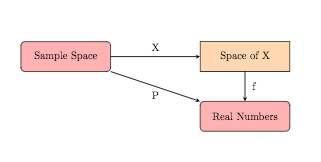
\includegraphics[width=\linewidth]{images/randomvariable.png}
\end{image}%
We will make various restrictions on the range of the \hyperref[x:definition:DefnRandomVariable]{random variable~{\xreffont\ref{x:definition:DefnRandomVariable}}} to fit different generalized problems. Then, we will be able to work on a problem (which may be inherently non-numerical) by using the random variable in subsequent calculations.%
\par
\begin{example}{Success vs Failure.}{g:example:idp202}%
When dealing with only two outcomes, one might use%
\begin{equation*}
S = \text{{ success, failure }}.
\end{equation*}
Choose%
\begin{gather*}
X( \text{success})=1\\
X( \text{failure})=0.
\end{gather*}
Then, \(R\) = \textbraceleft{}0,1\textbraceright{}.%
\end{example}
%
\par
\begin{example}{Standard Dice Pairs.}{g:example:idp203}%
When gambling with a pair of dice, one might use S=ordered pairs of all possible rolls.  Then%
\begin{equation*}
S = \text{ {(a,b): a=die 1 outcome, b=die 2 outcome}}.
\end{equation*}
Choose%
\begin{equation*}
X( (a,b) ) = a+b.
\end{equation*}
Then, \(R\) = \textbraceleft{}2, 3, 4, 5, ..., 12\textbraceright{}.%
\end{example}
%
\par
\begin{example}{Other Dice Options.}{g:example:idp204}%
When rolling dice in a board game (like RISK), one might use%
\begin{equation*}
S= \text{{ (a,b) : a=die 1 outcome, b=die 2 outcome}}
\end{equation*}
Choose%
\begin{equation*}
X( (a,b) ) = \text{max{a,b}}.
\end{equation*}
Then, \(R\) = \textbraceleft{}1, 2, 3, 4, 5, 6\textbraceright{}.%
\end{example}
%
\par
\begin{definition}{Countable and Uncountable Sets.}{g:definition:idp205}%
\(R\) contains a countable number of points if either \(R\) is finite or there is a one to one correspondence between R and the positive integers. Such a set will be called discrete. We will see that often the set \(R\) is not countable. If \(R\) consists of an interval of points (or a union of intervals), then we call X a continuous random variable.%
\end{definition}
%
\par
Notice that in each of the examples above, the space \(R\) was finite. Therefore, each of those random variables would be considered countable. One can however have random variables with a infinite number of values in \(R\) and yet still be countable.%
\par
\begin{example}{}{g:example:idp206}%
Consider the random variable \(X\) representing the number of coin flips \emph{until} you get a Heads.  Even though it is unlikely to have to keep on going, consider the fact that you \emph{could} continually flip and get Tails every time for a long time.  So, the possible values for \(X\) would be \(R\) = \textbraceleft{}1, 2, 3, 4, ... \textbraceright{} which is precisely the infinite set of positive integers.  Therefore, \(X\) is a countable random variable.%
\end{example}
%
\par
\begin{example}{}{g:example:idp207}%
Consider the random variable \(X\) representing the time until a light bulb fails to work after being successfully turned on.  Notice that the bulb \emph{could} fail in a relatively short time (near 0 let's say) or \emph{could} continue to last for almost eternity (or as long as you might want to measure).  However, time is measured on a continuum and therefore for this random variable \(X\) you would have \(R\) equal to the interval from 0 to infinity, i.e. \(R = (0,\infty)\) which is not a countable set.%
\end{example}
%
\end{sectionptx}
%
%
\typeout{************************************************}
\typeout{Section 5.3 Probability Functions}
\typeout{************************************************}
%
\begin{sectionptx}{Probability Functions}{}{Probability Functions}{}{}{x:section:ProbabilityFunctionsDefined}
In the formulas below, we will presume that we have a \hyperref[x:definition:DefnRandomVariable]{random variable~{\xreffont\ref{x:definition:DefnRandomVariable}}} \(X\) which maps the sample space S onto some range of real numbers \(R\).  From this set, we then can define a probability function \(f(x)\) which acts on the numerical values in \(R\) and returns another real number.  We attempt to do so to obtain (for discrete values) P(sample space value s)\(= f(X(s))\).  That is, the probability of a given outcome s is equal to the composition which takes s to a numerical value x which is then plugged into f to get the same final values.%
\par
For example, consider a random variable which assigns a 1 when you roll a 1 on a six-sided die and 0 otherwise. Presuming each side is equally likely, \(f(1) = \frac{1}{6}\) and \(f(0) = \frac{5}{6}\).%
\par
\begin{definition}{Probability "Mass" Function.}{x:definition:DefnPMF}%
Given a discrete \hyperref[x:definition:DefnRandomVariable]{random variable~{\xreffont\ref{x:definition:DefnRandomVariable}}} \(X\) on a space \(R\), a probability mass function on \(X\) is given by a function \(f:R \rightarrow \mathbb{R}\) such that:%
\begin{align*}
& \forall x \in R , f(x) \gt 0\\
& \sum_{x \in R} f(x) = 1\\
& A \subset R \Rightarrow P(X \in A) = \sum_{x \in A}f(x)
\end{align*}
For \(x \not\in R\), you can use the convention \(f(x)=0\).%
\end{definition}
%
\par
\begin{definition}{Probability "Density" Function.}{x:definition:DefnPDF}%
Given a continuous random variable \(X\) on a space \(R\), a probability density function on \(X\) is given by a function \(f:R \rightarrow \mathbb{R}\) such that:%
\begin{align*}
& \forall x \in R , f(x) \gt 0\\
& \int_{R} f(x) dx = 1\\
& A \subset R \Rightarrow P(X \in A) = \int_{A} f(x) dx
\end{align*}
For \(x \not\in R\), you can use the convention \(f(x)=0\).%
\end{definition}
%
\par
For the purposes of this book, we will use the term "Probability Function" to refer to either of these options.%
\par
\begin{example}{Discrete Probability Function.}{g:example:idp208}%
Consider \(f(x) = x/10\) over R = \textbraceleft{}1,2,3,4\textbraceright{}.  Then, f(x) is obviously positive for each of the values in R and certainly%
\begin{equation*}
\sum_{x \in R} f(x) = f(1) + f(2) + f(3) + f(4) = 1/10 + 2/10 + 3/10 + 4/10 = 1.
\end{equation*}
Therefore, f(x) is a probability mass function over the space \(R\).%
\end{example}
%
\par
\leavevmode%
\begin{sageinput}
# Combining all of the above into one interactive cell
@interact
def _(D = input_box([1,2,3,5,6,8,9,11,12,14],label="Domain (in brackets):"), 
       Probs = input_box([1/20,1/20,1/20,3/20,1/20,4/20,4/20,1/20,1/20,3/20],label=" $$f(x)$$ (in brackets):"),
       n_samples=slider(100,10000,100,100,label="# if samples:")):
    n = len(D)
    R = range(n)
    one_huh = sum(Probs)

    if one_huh!=1:
        print("f(x) values do not sum to 1")
    else:
        G = Graphics()
        if len(D)==len(Probs):
            f = zip(D,Probs)
            meanf = 0
            variancef = 0
            for k in R:
                meanf += D[k]*Probs[k]
                variancef += D[k]^2*Probs[k]
                G += line([(D[k],0),(D[k],Probs[k])],color='green')
            variancef = variancef - meanf^2
            sd = sqrt(variancef)
            G += points(f,color='blue',size=50)
            G += point((meanf,0),color='yellow',size=60,zorder=3)
            G += line([(meanf-sd,0),(meanf+sd,0)],color='red',thickness=5)
    
            g = DiscreteProbabilitySpace(D,Probs)
            pretty_print("     mean = %s"%str(meanf))
            pretty_print(" variance = %s"%str(variancef))
    
        #  perhaps to add mean and variance for pmf here
        else:
            print("Domain D and Probabilities Probs must be lists of the same size")
    
    #  Now, let's sample from the distribution given above and see how a random sampling matches up

        counts = [0] * len(Probs)
        X = GeneralDiscreteDistribution(Probs)
        sample = []

        for _ in range(n_samples):
            elem = X.get_random_element()
            sample.append(D[elem])
            counts[elem] += 1
        Empirical = [1.0*x/n_samples for x in counts] # random
    
        samplemean = mean(sample)
        samplevariance = variance(sample)
        sampdev = sqrt(samplevariance)
    
        E = points(zip(D,Empirical),color='orange',size=40)
        E += point((samplemean,0.005),color='brown',size=60,zorder=3)
        E += line([(samplemean-sampdev,0.005),(samplemean+sampdev,0.005)],color='orange',thickness=5)    
        (G+E).show(ymin=0,figsize=(8,5))
\end{sageinput}
%
\par
\begin{example}{Continuous Probability Function.}{g:example:idp209}%
Consider \(f(x) = x^2/c\) for some positive real number c and presume \(R\) = [-1,2]. Then f(x) is nonnegative (and only equals zero at one point). To make \(f(x)\) a \hyperref[x:definition:DefnPDF]{probability density function~{\xreffont\ref{x:definition:DefnPDF}}}, we must have%
\begin{equation*}
\int_{x \in R} f(x) = 1.
\end{equation*}
In this instance you get%
\begin{equation*}
1 = \int_{-1}^2 x^2/c = x^3/(3c) |_{-1}^2 = \frac{8}{3c} - \frac{-1}{3c} = \frac{3}{c}
\end{equation*}
Therefore, \(f(x)\) is a probability density function over \(R\) provided  \(c = 3\).%
\end{example}
%
\par
\begin{definition}{Distribution Function.}{x:definition:DefnDistributionFunction}%
Given a random variable \(X\) on a space \(R\), a probability distribution function on \(X\) is given by a function%
\begin{equation*}
F:\mathbb{R} \rightarrow \mathbb{R} \ni \displaystyle F(x)=P(X \le x).
\end{equation*}
%
\end{definition}
%
\par
\begin{example}{Discrete Distribution Function.}{g:example:idp210}%
Using \(f(x) = x/10\) over \(R\) = \textbraceleft{}1,2,3,4\textbraceright{} again, note that \(F(x)\) will only change at these four domain values. We get \begin{tableptx}{\textbf{Discrete Distribution Function Example}}{g:table:idp211}{}%
\centering
{\tabularfont%
\begin{tabular}{rr}
\multicolumn{1}{rB}{X}&F(x)\tabularnewline\hrulemedium
\multicolumn{1}{rB}{\(x \lt 1\)}&0\tabularnewline[0pt]
\multicolumn{1}{rB}{\(1 \le x \lt 2\)}&1\slash{}10\tabularnewline[0pt]
\multicolumn{1}{rB}{\(2 \le x \lt 3\)}&3\slash{}10\tabularnewline[0pt]
\multicolumn{1}{rB}{\(3 \le x \lt 4\)}&6\slash{}10\tabularnewline[0pt]
\multicolumn{1}{rB}{\(4 \le x \)}&1
\end{tabular}
}%
\end{tableptx}%
%
\end{example}
%
\par
\begin{example}{Continuous Distribution Function.}{g:example:idp212}%
Consider \(f(x) = x^2/3\) over \(R\) = [-1,2].  Then, for \(-1 \le x \le 2\),%
\begin{equation*}
F(x) = \int_{-1}^x u^2/3 du = x^3/9 + 1/9.
\end{equation*}
Notice, \(F(-1) = 0\) since nothing has yet been accumulated over values smaller than -1 and \(F(2) = 1\) since by that time everything has been accumulated. In summary: \begin{tableptx}{\textbf{Continuous Distribution Function Example}}{g:table:idp213}{}%
\centering
{\tabularfont%
\begin{tabular}{rr}
\multicolumn{1}{rB}{X}&F(x)\tabularnewline\hrulemedium
\multicolumn{1}{rB}{\(x \lt -1\)}&0\tabularnewline[0pt]
\multicolumn{1}{rB}{\(-1 \le x \lt 2\)}&\(x^3/9 + 1/9\)\tabularnewline[0pt]
\multicolumn{1}{rB}{\(2 \le x\)}&1
\end{tabular}
}%
\end{tableptx}%
%
\end{example}
%
\par
\begin{theorem}{}{}{x:theorem:theorem-Fmin}%
\(F(x)=0, \forall x \lt \inf(R)\) where inf is the infimum...the "minimum" but in a limit sense.%
\end{theorem}
\begin{proof}{}{g:proof:idp214}
Let a = inf(\(R\)). Then, for \(x \lt a,\)%
\begin{equation*}
F(x) = P(X \le x) \le P(X \lt a) = 0
\end{equation*}
since none of the x-values in this range are in \(R\).%
\end{proof}
%
\par
\begin{theorem}{}{}{x:theorem:theorem-Fmax}%
\(F(x)=1, \forall x \ge \sup(R)\) where sup is the supremum...the "maximum" but in a limit sense.%
\end{theorem}
\begin{proof}{}{g:proof:idp215}
Let b = sup(\(R\)). Then, for \(x \ge b,\)%
\begin{equation*}
F(x) = P(X \le x)  = P(X \le b) + P( b \lt X \le x) = P(X \le b) = 1
\end{equation*}
since all of the x-values in this range are in R and therefore will either sum over or integrate over all of \(R\).%
\end{proof}
%
\par
\begin{theorem}{}{}{g:theorem:idp216}%
\(F\) is non-decreasing%
\end{theorem}
\begin{proof}{}{g:proof:idp217}
Case 1: \(R\) discrete%
\begin{align*}
\forall x_1,x_2 \in \mathbb{Z} \ni x_1 \lt x_2\\
F(x_2) & = \sum_{x \le x_2} f(x) \\
& = \sum_{x \le x_1} f(x) + \sum_{x_1 \lt x \le x_2} f(x)\\
& \ge \sum_{x \le x_1} f(x) = F(x_1)
\end{align*}
%
\par
Case 2: \(R\) continuous%
\begin{align*}
\forall x_1,x_2 \in \mathbb{R} \ni x_1 \lt x_2\\
F(x_2) & = \int_{-\infty}^{x_2} f(x) dx \\
& = \int_{-\infty}^{x_1} f(x) dx + \int_{x_1}^{x_2} f(x) dx\\
& \ge \int_{-\infty}^{x_1} f(x) dx\\
& = F(x_1)\qedhere
\end{align*}
%
\end{proof}
%
\par
\begin{theorem}{Using Discrete Distribution Function to compute probabilities.}{}{x:theorem:theorem-Fvsf-discrete}%
For \(x \in R, f(x) = F(x) - F(x-1)\)%
\end{theorem}
\begin{proof}{}{g:proof:idp218}
Assume \(x \in R\) for some discrete \(R\). Then,%
\begin{equation*}
F(x) - F(x-1) = \sum_{u \le x} f(u) - \sum_{u \lt x} f(u) = f(x)\qedhere
\end{equation*}
%
\end{proof}
%
\par
\begin{theorem}{Using Continuous Distribution function to compute probabilities.}{}{x:theorem:theorem-Fvsf-continuous}%
For \(a \lt b, (a,b) \in R, P(a \lt X \le b) = F(b) - F(a)\)%
\end{theorem}
\begin{proof}{}{g:proof:idp219}
For a and b as noted, consider%
\begin{align*}
F(b) - F(a) & = \int_{-\infty}^b f(x) dx - \int_{-\infty}^a f(x) dx\\
& = \int_a^b f(x) dx \\
& = P(a \lt x \le b)\qedhere
\end{align*}
%
\end{proof}
%
\par
\begin{corollary}{}{}{x:corollary:corollary-ProbPointZero-continuous}%
For continuous distributions, \(P(X = a) = 0\).%
\end{corollary}
\begin{proof}{}{g:proof:idp220}
We will assume that \(F(x)\) is a continuous function. With that assumption, note%
\begin{equation*}
P(a-\epsilon \lt  x \le a)  = \int_{a-\epsilon}^a f(x) dx = F(a) - F(a-\epsilon)
\end{equation*}
Take the limit as \(\epsilon \rightarrow 0^+\) to get the result noting that%
\end{proof}
%
\par
\begin{theorem}{\(F(x)\) vs \(f(x)\), for continuous distributions.}{}{g:theorem:idp221}%
If \(X\) is a continuous random variable, \(f\) the corresponding probability function, and \(F\) the associated distribution function, then%
\begin{equation*}
f(x) = F'(x)
\end{equation*}
%
\end{theorem}
\begin{proof}{}{g:proof:idp222}
Assume \(X\) is continuous and \(f\) and \(F\) as above. Notice, by the definition of \(f\), \(\lim_{x \rightarrow \pm \infty} f(x) = 0\) since otherwise the integral over the entire space could not be finite.%
\par
Now, let \(A(x)\) be any antiderivative of \(f(x)\). Then, by the Fundamental Theorem of Calculus,%
\begin{align*}
F(x) & = \int_{-\infty}^x f(u) du\\
& = A(x) - \lim_{u \rightarrow -\infty} A(u)
\end{align*}
Hence, \(F'(x) = A'(x) - \lim_{u \rightarrow -\infty} A'(u) = f(x)\) as desired.%
\end{proof}
%
\par
\begin{definition}{Percentiles for Random Variables.}{x:definition:DefnPercentileRandomVariable}%
For \(0 \lt p \lt 1\), the \(100p^{th}\) percentile is the largest random variable value c that satisfies%
\begin{equation*}
F(c) = p.
\end{equation*}
For continuous random variables over an interval \(R = [a,b]\), you will solve for c in the equation%
\begin{equation*}
\int_a^c f(x) dx.
\end{equation*}
For discrete random variables, it is unlikely that a particular percentile will land exactly on one of the elements of \(R\) but you will want to take the smallest value in \(R\) so that \(F(c) \ge p\).%
\par
The 50th percentile (as before) is also known as the median.%
\end{definition}
%
\par
\begin{example}{Continuous Percentile.}{g:example:idp223}%
For our earlier example with \(f(x) = x^2/3\) on R = [-1,2], the 50th percentile (i.e. the median) is found by starting with p = 0.5 and then solving%
\begin{equation*}
F(c) = 0.5
\end{equation*}
or%
\begin{equation*}
c^3/9 + 1/9 = 1/2
\end{equation*}
or%
\begin{equation*}
c^3 + 1 = 9/2.
\end{equation*}
After solving for c, you find%
\begin{equation*}
\text{median} = \sqrt[3]{7/2} \approx 1.518.
\end{equation*}
%
\end{example}
%
\par
\begin{example}{Discrete Percentile.}{g:example:idp224}%
TBA, using one of the table examples from above.%
\end{example}
%
\end{sectionptx}
%
%
\typeout{************************************************}
\typeout{Section 5.4 Expected Value}
\typeout{************************************************}
%
\begin{sectionptx}{Expected Value}{}{Expected Value}{}{}{x:section:ExpectedValue}
Blaise Pascal was a 	17th century mathematician and philosopher who was accomplished in many areas but may likely be best known to you for his creation of what is now known as Pascal's Triangle. As part of his philosophical pursuits, he proposed what is known as "Pascal's wager". It suggests two  mutually exclusive outcomes: that God exists or that he does not. His argument is that a rational person should live as though God exists and seek to believe in God. If God does not actually exist, such a person will have only a finite loss (some pleasures, luxury, etc.), whereas they stand to receive infinite gains as represented by eternity in Heaven and avoid an infinite losses of eternity in Hell. This type of reasoning is part of what is known as "decision theory".%
\par
You may not confront such dire payouts when making your daily decisions but we need a formal method for making these determinations precise. The procedure for doing so is what we call expected value.%
\par
\begin{definition}{Expected Value.}{x:definition:DefnExpectedValue}%
Given a random variable \(X\) over space \(R\), corresponding probability function \(f(x)\) and "value function" \(v(x)\), the expected value of \(v(x)\) is given by%
\begin{equation*}
E = E[v(X)] = \sum_{x \in R} v(x) f(x)
\end{equation*}
provided \(X\) is discrete, or%
\begin{equation*}
E = E[v(X)] = \int_R v(x)f(x) dx
\end{equation*}
provided \(X\) is continuous.%
\end{definition}
%
\par
\begin{theorem}{Expected Value is a Linear Operator.}{}{g:theorem:idp225}%
%
\begin{enumerate}
\item{}\(\displaystyle E[c] = c\)%
\item{}\(\displaystyle E[c v(X)] = c E[v(X)]\)%
\item{}\(\displaystyle E[v(X) + w(X)] = E[v(X)] + E[w(X)]\)%
\end{enumerate}
%
\end{theorem}
\begin{proof}{}{g:proof:idp226}
Each of these follows by utilizing the corresponding linearity properties of the summation and integration operations. For example, to verify part three in the continuous case:%
\begin{align*}
E[v(X) + w(X)] & = \int_{x \in R} [v(x)+w(x)]f(x) dx\\
& = \int_{x \in R} v(x)f(x) dx + \int_{x \in R} w(x)f(x) dx\\
& = E[v(X)] + E[w(X)].\qedhere
\end{align*}
%
\end{proof}
%
\begin{inlineexercise}{WebWork - Expected Value.}{g:exercise:idp227}%
If \(E[X]=4\) and \(\mbox{Var}(X) = 1\), then%
\par
\(E[(4 + 5 X)^2] =\)\fillin{18.1818181818182}%
\par
and%
\par
\(\mbox{Var}(3 + 5 X) =\)\fillin{18.1818181818182}.%
\par\smallskip%
\noindent\textbf{\blocktitlefont Answer 1}.\hypertarget{g:answer:idp228}{}\quad{}\(601\)%
\par\smallskip%
\noindent\textbf{\blocktitlefont Answer 2}.\hypertarget{g:answer:idp229}{}\quad{}\(25\)%
\end{inlineexercise}%
\begin{example}{Discrete Expected Value.}{g:example:idp230}%
Consider \(f(x) = x/10\) over \(R\) = \textbraceleft{}1,2,3,4\textbraceright{} where the payout is 10 euros if x=1, 5 euros if x=2, 2 euros if x=3 and -7 euros if x = 4.  Then your value function would be%
\begin{equation*}
v(1)=10, v(2) = 5, v(3)=2, v(4) = -7.
\end{equation*}
Computing the expect payout gives%
\begin{equation*}
E = 10 \times 1/10 + 5 \times 2/10 + 2 \times 3/10 - 7 \times 4/10 = -2/10
\end{equation*}
Therefore, the expected payout is actually negative due to a relatively large negative payout associated with the largest likelihood outcome and the larger positive payout only associated with the least likely outcome.%
\end{example}
%
\par
\begin{example}{Continuous Expected Value.}{x:example:ContinuousEV-example}%
Consider \(f(x) = x^2/3\) over \(R\) = [-1,2] with value function given by \(v(x) = e^x - 1\). Then, the expected value for \(v(x)\) is given by%
\begin{equation*}
E = \int_{-1}^2 (e^x-1) \cdot x^2/3 = -1/9 \cdot (e + 15) \cdot e^{-1} + 2/3 \cdot e^2 - 8/9 \approx 3.3129
\end{equation*}
%
\end{example}
%
\par
\begin{definition}{Theoretical Measures.}{x:definition:TheoreticalMeasures}%
Given a random variable with probability function f(x) over space R%
\begin{enumerate}
\item\hypertarget{x:li:TheoreticalMean}{}The mean of \(X = \mu = E[x]\)%
\item\hypertarget{x:li:TheoreticalVariance}{}The variance of \(X = \sigma^2 = E[(x-\mu)^2]\)%
\item\hypertarget{x:li:TheoreticalSkewness}{}The skewness of \(X = \gamma_1 = \frac{E[(x-\mu)^3]}{\sigma^3}\)%
\item\hypertarget{x:li:TheoreticalKurtosis}{}The kurtosis of \(X = \gamma_2 = \frac{E[(x-\mu)^4]}{\sigma^4}\)%
\end{enumerate}
%
\end{definition}
%
\par
\begin{theorem}{Alternate Formulas for Theoretical Measures.}{}{x:theorem:TheoreticalMeasuresAlternates}%
%
\begin{enumerate}
\item\hypertarget{x:li:TheoreticalMeasuresAlternatesVar}{}\(\displaystyle \sigma^2 = E[x^2] - \mu^2 = E[X(x-1)] + \mu - \mu^2\)%
\item\hypertarget{x:li:TheoreticalMeasuresAlternatesSkew}{}\(\displaystyle \gamma_1 = \frac{1}{\sigma^3} \cdot \left [ E[X^3] - 3 \mu E[X^2] + 2\mu^3 \right ]\)%
\item\hypertarget{x:li:TheoreticalMeasuresAlternatesKurt}{}\(\displaystyle \gamma_2 = \frac{1}{\sigma^4} \cdot \left [ E[X^4] - 4 \mu E[X^3] + 6\mu^2 E[X^2] - 3 \mu^4 \right ]\)%
\end{enumerate}
%
\end{theorem}
\begin{proof}{}{g:proof:idp231}
In each case, expand the binomial inside and use the linearity of expected value.%
\end{proof}
%
\par
Consider the following example when computing these statistics for a discrete variable. In this case, we will utilize a variable with a relatively small space so that the summations can be easily done by hand. Indeed, consider \begin{tableptx}{\textbf{Discrete Probability Function Example}}{g:table:idp232}{}%
\centering
{\tabularfont%
\begin{tabular}{rr}
\multicolumn{1}{rB}{X}&f(x)\tabularnewline\hrulemedium
\multicolumn{1}{rB}{0}&0.10\tabularnewline[0pt]
\multicolumn{1}{rB}{1}&0.25\tabularnewline[0pt]
\multicolumn{1}{rB}{2}&0.40\tabularnewline[0pt]
\multicolumn{1}{rB}{4}&0.15\tabularnewline[0pt]
\multicolumn{1}{rB}{7}&0.10
\end{tabular}
}%
\end{tableptx}%
 \begin{image}{0}{1}{0}%
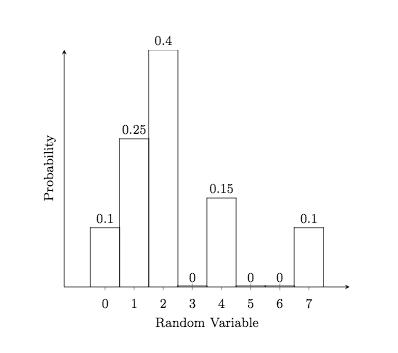
\includegraphics[width=\linewidth]{images/DiscreteHistogramExample.png}
\end{image}%
%
\par
Using the definition of \hyperlink{x:li:TheoreticalMean}{mean~{\xreffont 1}} as a sum,%
\begin{align*}
\mu & = 0 \cdot 0.10 + 1 \cdot 0.25 + 2 \cdot 0.40 + 4 \cdot 0.15 + 7 \cdot 0.10\\
& = 0 + 0.25 + 0.80 + 0.60 + 0.70\\
& = 2.35
\end{align*}
Notice where this lies on the probability histogram for this distribution.%
\par
For the \hyperlink{x:li:TheoreticalVariance}{variance~{\xreffont 2}} and using \hyperlink{x:li:TheoreticalMeasuresAlternatesVar}{the alternate formulation~{\xreffont 1}}%
\begin{align*}
\sigma^2 & = E[X^2] - \mu^2\\
& = \left [ 0^2 \cdot 0.10 + 1^2 \cdot 0.25 + 2^2 \cdot 0.40 + 4^2 \cdot 0.15 + 7^2 \cdot 0.10 \right ] - 2.35^2\\
& = 0 + 0.25 + 1.60 + 2.40 + 4.90 - 5.5225\\
& = 9.15 - 5.225\\
& = 3.6275 
\end{align*}
and so the standard deviation \(\sigma = \sqrt{3.6275} \approx 1.90\). Notice that 4 times this value encompasses almost all of the range of the distribution.%
\par
For the \hyperlink{x:li:TheoreticalSkewness}{skewness~{\xreffont 3}} and using \hyperlink{x:li:TheoreticalMeasuresAlternatesSkew}{the alternate formulation~{\xreffont 2}}%
\begin{align*}
\text{Numerator = } & E[X^3] - 3 \mu E[X^2] + 2\mu^3\\
& = \left [ 0^3 \cdot 0.10 + 1^3 \cdot 0.25 + 2^3 \cdot 0.40 + 4^3 \cdot 0.15 + 7^3 \cdot 0.10 \right ] - 3 \cdot 2.35 \cdot 9.15 + 2 \cdot 2.35^3\\
& \approx 0 + 0.25 + 3.20 + 9.60 + 34.3 - 64.5075 + 25.96\\
& = 47.35 - 64.5075 + 25.96\\
& \approx 8.80
\end{align*}
which yields a skewness of \(\gamma_1 = 8.80 / \sigma^3 \approx 1.27 \). This indicates a slight skewness to the right of the mean. You can notice the 4 and 7 entries on the histogram illustrate a slight trailing off to the right.%
\par
Finally, for \hyperlink{x:li:TheoreticalKurtosis}{kurtosis~{\xreffont 4}} and using \hyperlink{x:li:TheoreticalMeasuresAlternatesKurt}{the alternate formulation~{\xreffont 3}}%
\begin{align*}
\text{Numerator = } & E[X^4] - 4 \mu E[X^3] + 6 \mu^2 E[X^2] - 3\mu^4\\
& = \left [ 0^4 \cdot 0.10 + 1^4 \cdot 0.25 + 2^4 \cdot 0.40 + 4^4 \cdot 0.15 + 7^4 \cdot 0.10 \right ] - 4 \cdot 2.35 \cdot 47.35 + 6 \cdot 2.35^2 \cdot 9.15^2 - 3 \cdot 2.35^4\\
& \approx 0 + 0.25 + 6.40 + 38.4 + 240.1 - 445.09 + 303.19 - 91.49\\
& \approx 285.15 - 445.09 + 303.19 - 91.49\\
& \approx 51.75
\end{align*}
which yields a kurtosis of \(\gamma_2 = 51.75 / \sigma^4 \approx 3.93\) which also notes that the data appears to have a modestly bell-shaped distribution.%
\begin{inlineexercise}{WebWork - Random Variables.}{g:exercise:idp233}%
Find the expected value for the random variable:%
\begin{sidebyside}{1}{0}{0}{0}%
\begin{sbspanel}{1}%
{\centering%
{\tabularfont%
\begin{tabular}{BlBlBlBlBlB}\hrulemedium
\(X\)&3&5&6&8\tabularnewline\hrulemedium
\(P(X)\)&0.21&0.16&0.25&0.38\tabularnewline\hrulemedium
\end{tabular}
}%
\par}
\end{sbspanel}%
\end{sidebyside}%
\par
\(E(X) =\) \fillin{9.090909090909092}%
\par\smallskip%
\noindent\textbf{\blocktitlefont Answer}.\hypertarget{g:answer:idp234}{}\quad{}\(5.97\)%
\end{inlineexercise}%
\begin{inlineexercise}{WebWork - More Random Variables.}{g:exercise:idp235}%
Prizes and the chances of winning in a sweepstakes are given in the table below.%
\begin{sidebyside}{1}{0}{0}{0}%
\begin{sbspanel}{1}%
{\centering%
{\tabularfont%
\begin{tabular}{BlBlB}\hrulemedium
Prize&Chances\tabularnewline\hrulemedium
\textdollar{}10,000,000&1 chance in 300,000,000\tabularnewline\hrulemedium
\textdollar{}350,000&1 chance in 150,000,000\tabularnewline\hrulemedium
\textdollar{}50,000&1 chance in 80,000,000\tabularnewline\hrulemedium
\textdollar{}20,000&1 chance in 5,000,000\tabularnewline\hrulemedium
\textdollar{}500&1 chance in 800,000\tabularnewline\hrulemedium
A watch valued at \textdollar{}60&1 chance in 7,000\tabularnewline\hrulemedium
\end{tabular}
}%
\par}
\end{sbspanel}%
\end{sidebyside}%
\par
(a) \(\) Find the expected value (in dollars) of the amount won by one entry.%
\par
(b) \(\) Find the expected value (in dollars) if the cost of entering this sweepstakes is the cost of a postage stamp (34 cents)%
\par\smallskip%
\noindent\textbf{\blocktitlefont Answer 1}.\hypertarget{g:answer:idp236}{}\quad{}\(0.0494880952380952\)%
\par\smallskip%
\noindent\textbf{\blocktitlefont Answer 2}.\hypertarget{g:answer:idp237}{}\quad{}\(-0.290511904761905\)%
\par\smallskip%
\noindent\textbf{\blocktitlefont Solution}.\hypertarget{g:solution:idp238}{}\quad{}\(W\) be the amount of money (in dollars) won by an entry.  Then%
\begin{equation*}
\begin{aligned}
E[W]  = \amp 10000000\cdot P(W = 10000000) + 350000 \cdot P(W = 350000) +  50000 \cdot P(W = 50000)\\
\amp  + \, 20000 \cdot P(W = 20000) +500 \cdot P( W = 500) + 60 \cdot P( W = 60)\\
\amp  = \frac{10000000}{300000000} + \frac{350000}{150000000} + \frac{50000}{80000000} + \frac{20000}{5000000} + \frac{500}{800000} + \frac{60}{7000} \\
\amp = 0.0494880952380952
\end{aligned}
\end{equation*}
So the expected value of the amount won by one entry in the sweepstakes is about 5 cents. (b) Let \(X\) be the net earnings from one entry into the sweepstakes.  Then \(X = W - 0.34\), so%
\begin{equation*}
E[X] = E[W- 0.34] = E[W] - 0.34 = -0.290511904761905.
\end{equation*}
\end{inlineexercise}%
\begin{inlineexercise}{WebWork - Even More.}{g:exercise:idp239}%
The table below summarizes the number of surface flaws found on the paintwork of new cars following their inspection after primer paint was applied by a new method:%
\begin{sidebyside}{1}{0}{0}{0}%
\begin{sbspanel}{1}%
{\centering%
{\tabularfont%
\begin{tabular}{BlBlB}\hrulemedium
No. of flaws&No. of cars\tabularnewline\hrulemedium
0&3\tabularnewline\hrulemedium
1&7\tabularnewline\hrulemedium
2&12\tabularnewline\hrulemedium
3&11\tabularnewline\hrulemedium
4&3\tabularnewline\hrulemedium
5&2\tabularnewline\hrulemedium
6&2\tabularnewline\hrulemedium
\end{tabular}
}%
\par}
\end{sbspanel}%
\end{sidebyside}%
\par
\alert{Part a)} Find the mean number of flaws per car. Please give your answer to two decimal places.%
\par
The mean number of flaws per car is: \fillin{2.727272727272727}%
\par
\alert{Part b)}%
\par
Find the variance of the number of flaws per car. Please give your answer to two decimal places.%
\par
The variance of the number of flaws per car is: \fillin{2.727272727272727}%
\par\smallskip%
\noindent\textbf{\blocktitlefont Answer 1}.\hypertarget{g:answer:idp240}{}\quad{}\(2.45\)%
\par\smallskip%
\noindent\textbf{\blocktitlefont Answer 2}.\hypertarget{g:answer:idp241}{}\quad{}\(2.151\)%
\par\smallskip%
\noindent\textbf{\blocktitlefont Solution}.\hypertarget{g:solution:idp242}{}\quad{}Here \(n = 40\) and the sample mean is%
\begin{equation*}
\bar{x} = 
\frac{3\times 0 +
7\times 1 +
12\times 2 +
11\times 3 +
3\times 4 +
2\times 5 +
2\times 6}
{40} \\
= 2.45.
\end{equation*}
%
\par
The sample variance is%
\par
%
\begin{equation*}
\frac{3\left( 0 - 2.45 \right) ^{2} +
7\left( 1 - 2.45 \right) ^{2} +
12\left( 2 - 2.45 \right) ^{2} +
11\left( 3 - 2.45 \right) ^{2} +
3\left( 4 - 2.45 \right) ^{2} + 
2\left( 5 - 2.45 \right) ^{2} +
2\left( 6 - 2.45 \right) ^{2}}
{39}
\end{equation*}
which is 2.151.%
\end{inlineexercise}%
Consider the following example when computing these statistics for a continuous variable. Let \(f(x) = \frac{3}{4} \cdot (1-x^2)\) over \(R = [-1,1]\). \begin{image}{0}{1}{0}%
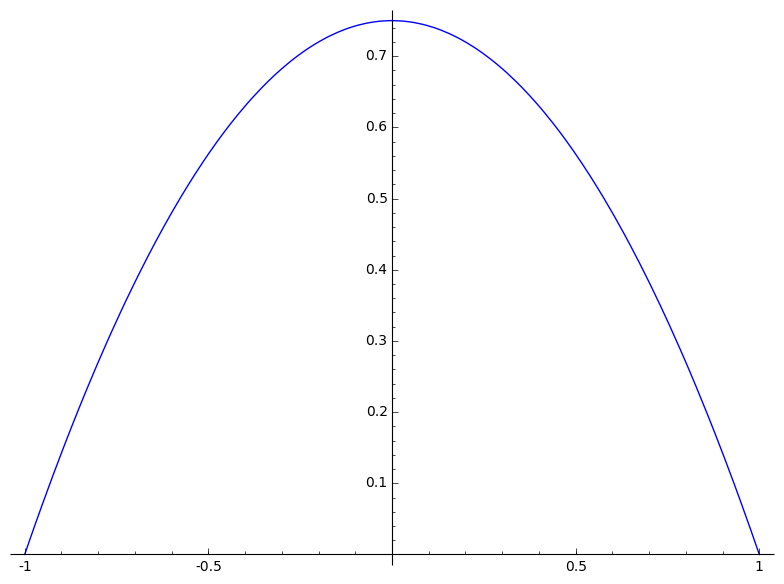
\includegraphics[width=\linewidth]{images/ContinuousDistributionExample.png}
\end{image}%
%
\par
Then for the \hyperlink{x:li:TheoreticalMean}{mean~{\xreffont 1}}%
\begin{align*}
\mu & = \int_{-1}^1 x \cdot \frac{3}{4} \cdot (1-x^2) dx\\
& = \int_{-1}^1 \frac{3}{4} \cdot (x-x^3) dx\\
& = \frac{3}{4} \cdot (x^2/2-x^4/4) \big |_{-1}^1\\
& = \frac{3}{4} \cdot [(1/2)-(1/4)] - [(1/2) - (1/4)]\\
& = 0
\end{align*}
as expected since the probability function is symmetric about x=0.%
\par
For the \hyperref[x:theorem:TheoreticalMeasuresAlternates]{variance~{\xreffont\ref{x:theorem:TheoreticalMeasuresAlternates}}}%
\begin{align*}
\sigma^2 & = \int_{-1}^1 x^2 \cdot \frac{3}{4} \cdot (1-x^2) dx - \mu^2\\
& = \int_{-1}^1 \cdot \frac{3}{4} \cdot (x^2-x^4) dx - 0\\
& = \frac{3}{4} \cdot (x^3 /3 -x^5 / 5) \big |_{-1}^1\\
& = \frac{3}{4} \cdot 2 \cdot (1/3-1/5)\\
& = \frac{3}{4} \cdot \frac{4}{15}\\
& = \frac{1}{5}
\end{align*}
and taking the square root gives a standard deviation slightly less than 1\slash{}2. Notice that four times this value encompasses almost all of the range of the distribution.%
\par
For the \hyperlink{x:li:TheoreticalSkewness}{skewness~{\xreffont 3}}, notice that the graph is symmetrical about the mean and so we would expect a skewness of 0.  Just to check it out%
\begin{align*}
\text{Numerator = } & E[X^3] - 3 \mu E[X^2] + 2\mu^3\\
& = \int_{-1}^1 x^3 \cdot \frac{3}{4} \cdot (1-x^2) dx - 3 E[X^2] \cdot 0 + 0^3 \\
& = \int_{-1}^1 \cdot \frac{3}{4} \cdot (x^3-x^5) dx\\
& = \frac{3}{4} \cdot (x^4/4-x^6/6) \big |_{-1}^1\\
& = 0
\end{align*}
as expected without having to actually complete the calculation by dividing by the cube of the standard deviation.%
\par
Finally, note that the probability function in this case is modestly close to a bell shaped curve so we would expect a \hyperlink{x:li:TheoreticalKurtosis}{kurtosis~{\xreffont 4}} and using \hyperlink{x:li:TheoreticalKurtosis}{the alternate formulation~{\xreffont 4}} in the vicinity of 3. Indeed, noting that (conveniently) \(\mu = 0\) gives%
\begin{align*}
\text{Numerator = } & E[X^4] - 4 \mu E[X^3] + 6 \mu^2 E[X^2] - 3 \mu^4\\
& = \int_{-1}^1 x^4 \cdot \frac{3}{4} \cdot (1-x^2) dx\\
& = \frac{3}{4} \cdot (x^5 /5-x^7 /7) \big |_{-1}^1\\
& = \frac{3}{4} \cdot 2(1/5-1/7)\\
& = \frac{3}{35}
\end{align*}
and so by dividing by \(\sigma^4 = \sqrt{\frac{1}{5}}^4 = \frac{1}{25}\) gives a kurtosis of%
\begin{equation*}
\gamma_2 = \frac{3}{35} / \frac{1}{25} = \frac{75}{35} \approx 2.14.
\end{equation*}
%
\par
\begin{example}{}{g:example:idp243}%
Consider \hyperref[x:example:ContinuousEV-example]{our previous example~{\xreffont\ref{x:example:ContinuousEV-example}}}. To compute the \hyperlink{x:li:TheoreticalMean}{mean~{\xreffont 1}} and \hyperlink{x:li:TheoreticalVariance}{variance~{\xreffont 2}} (and hence the standard deviation) for this distribution,%
\begin{equation*}
\mu = \int_{-1}^2 x \cdot x^2/3 dx = \int_{-1}^2 x^3/3 dx = \frac{2^4}{12} - \frac{(-1)^4}{12} = \frac{15}{12} = \frac{5}{4}
\end{equation*}
and by using \hyperref[x:theorem:TheoreticalMeasuresAlternates]{the alternate formulas~{\xreffont\ref{x:theorem:TheoreticalMeasuresAlternates}}}%
\begin{align*}
\sigma^2 & = E[X^2] - \mu^2\\
& = \int_{-1}^2 x^2 \cdot x^2/3 \; dx - \mu^2\\
& = \int_{-1}^2 x^4/3 \; dx - \left ( \frac{5}{4} \right )^2\\
& = \frac{2^5}{15} - \frac{(-1)^5}{15} - \frac{25}{16}\\
& = \frac{33}{15} - \frac{25}{16} = \frac{51}{80}
\end{align*}
which gives%
\begin{equation*}
\sigma = \sqrt{\frac{51}{80}} \approx 0.7984.
\end{equation*}
%
\par
For \hyperlink{x:li:TheoreticalSkewness}{skewness~{\xreffont 3}}, note that in computing the variance above you also found that%
\begin{equation*}
E[X^2] = \frac{11}{5}.
\end{equation*}
So, once again by using \hyperref[x:theorem:TheoreticalMeasuresAlternates]{the alternate forumulas~{\xreffont\ref{x:theorem:TheoreticalMeasuresAlternates}}}%
\begin{equation*}
E[X^3] = \int_{-1}^2 x^3 \cdot x^2/3 dx = \frac{x^6}{18} |_{-1}^2 = \frac{7}{2}
\end{equation*}
and so%
\begin{equation*}
\gamma_1 = \frac{\frac{7}{2} - 3 \cdot \frac{5}{4} \cdot \frac{11}{5} + 2 \cdot (\frac{5}{4})^3}{\sqrt{\frac{51}{80}}^3}
\end{equation*}
%
\par
For \hyperlink{x:li:TheoreticalKurtosis}{kurtosis~{\xreffont 4}}, you can reuse \(E[X^3] = \frac{7}{2}\) and \(E[X^2] = \frac{11}{5}\) and \hyperref[x:theorem:TheoreticalMeasuresAlternates]{the alternate forumulas~{\xreffont\ref{x:theorem:TheoreticalMeasuresAlternates}}} to determine%
\begin{equation*}
E[(X-\mu)^4] = E[X^4] - 4 \mu \cdot E[X^3] + 6 \mu^2 \cdot E[X^2] - 3 \mu^4
\end{equation*}
which is the numerator for the kurtosis.%
\end{example}
%
\par
\begin{example}{Roulette.}{g:example:idp244}%
Roulette is a gambling game popular in may casinos in which a player attempts to win money from the casino by predicting the location that a ball lands on in a spinning wheel.  There are two variations of this game...the American version and the European version. The difference being that the American version has one additional numbered slot on the wheel. The American version of the game will be used for the purposes of this example.%
\par
A Roulette wheel consists of 38 equally-sized sectors identified with the numbers 1 through 36 plus 0 and 00. The 0 and 00 sectors are colored green and half of the remaining numbers are in sectors colored red with the remainder colored black.  A steel ball is dropped onto a spinning wheel and as the wheel comes to rest the sector in which it comes to rest is noted.  It is easy to determine that the probability of landing on any one of the 38 sectors is 1\slash{}38. A picture of a typical American-style wheel and betting board is given by \begin{image}{0}{1}{0}%
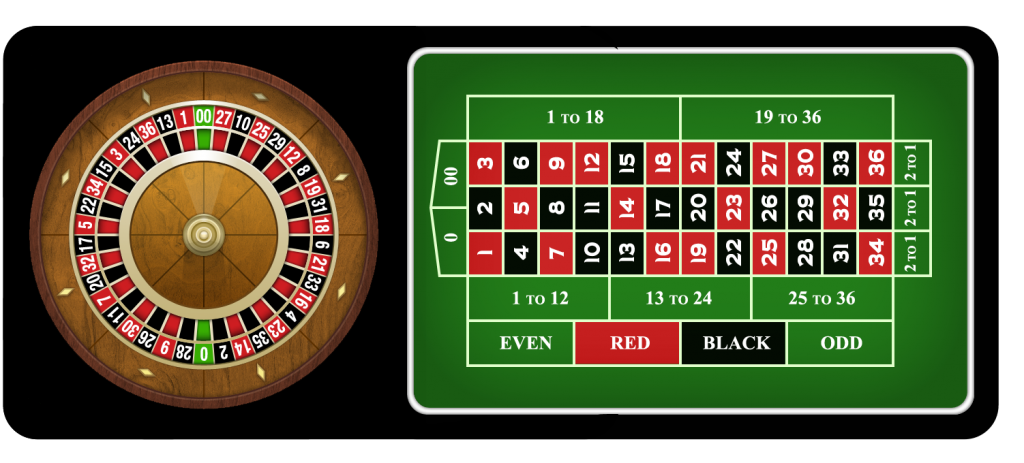
\includegraphics[width=\linewidth]{images/6-1-American-Roulette-1024x463.png}
\end{image}%
. (Found at BigFishGames.com.)%
\par
Since this is a game in a casino, there must be the opportunity to bet (and likely lose) money. For the remainder of this example we will assume that you are betting 1 dollar each time. If you were to bet more then the values would scale correspondingly. However, if you place your bet on any single number and the ball ends up on the sector corresponding to that number, you win a net of 35 dollars.  If the ball lands elsewhere you lose your dollar. Therefore the expected value of winning if you bet on one number is%
\begin{equation*}
E[\text{win on one}] = 35 \cdot \frac{1}{38} - 1 \cdot \frac{37}{38} = - \frac{2}{38}
\end{equation*}
which is a little more than a nickel loss on average.%
\par
You can bet on two numbers as well and if the ball lands on either of the two then you win a payout in this case of 17 dollars.  Therefore the expected value of winning if you bet on two numbers is%
\begin{equation*}
E[\text{win on two numbers}] = 17 \cdot \frac{2}{38} - 1 \cdot \frac{36}{38} = - \frac{2}{38}.
\end{equation*}
%
\par
Continuing, you can bet on three numbers and if the ball lands on any of the three then you win a payout of 11 dollars.  Therefore the expected value of winning if you bet on three numbers is%
\begin{equation*}
E[\text{win on three numbers}] = 11 \cdot \frac{3}{38} - 1 \cdot \frac{35}{38} = - \frac{2}{38}.
\end{equation*}
%
\par
You can bet on all reds, all blacks, all evens (ignoring 0 and 00), or all odds and get your dollar back. The expected value for any of these options is%
\begin{equation*}
E[\text{win on eighteen numbers}] = 1 \cdot \frac{18}{38} - 1 \cdot \frac{20}{38} = - \frac{2}{38}.
\end{equation*}
%
\par
There is one special way to bet which uses the the 5 numbers \textbraceleft{}0, 00, 1, 2, 3\textbraceright{} and pays 6 dollars. This is called the "top line of basket".  Notice that the use of five numbers will make getting the same expected value as the other cases impossible using regular dollars and cents. The expected value of winning in this case us%
\begin{equation*}
E[\text{win on top line of basket}] = 6 \cdot \frac{5}{38} - 1 \cdot \frac{33}{38} = - \frac{3}{38}
\end{equation*}
which is of course worse and is the only normal way to bet on roulette which has a different expected value.%
\par
There are other possible ways to bet on roulette but none provide a better expected value of winning.  The moral of this story is that you should never bet on the 5 number option and if you ever get ahead by winning on roulette using any of the possible options then you should probably stop quickly since over a long period of time it is expected that you will lose an average of \(\frac{1}{19}\) dollars per game.%
\end{example}
%
\par
Going back to Pascal's wager, let%
\begin{itemize}[label=\textbullet]
\item{}X = 0 represent disbelief when God doesn't exist%
\item{}X = 1 represent disbelief when God does exist%
\item{}X = 2 represent belief when God does exist%
\item{}X = 3 represent belief when God does not exist%
\end{itemize}
Presume that p is the likelihood that God exists. Then you can compute the expected value of disbelief and the expect value of belief by first creating a value function. Below, for argument sake we are somewhat randomly assign a value of one million to disbelief if God doesn't exist. The conclusions are the same if you choose any other finite number...%
\begin{gather*}
v(0) = 1,000,000, f(0) = 1-p\\
v(1) = -\infty, f(1) = p\\
v(2) = \infty, f(2) = p\\
v(3) = 0, f(3) = 1-p
\end{gather*}
Then,%
\begin{align*}
E[\text{disbelief}] & = v(0)f(0) + v(1)f(1)\\
& = 1000000 \times (1-p) - \infty \times p\\
& = -\infty
\end{align*}
if p\textgreater{}0. On the other hand,%
\begin{align*}
E[\text{belief}] & = v(2)f(2) + v(3)f(3)\\
& = \infty \times p + 0 \times (1-p)\\
& = \infty
\end{align*}
if p\textgreater{}0. So Pascal's conclusion is that if there is even the slightest chance that God exists then belief is the smart and scientific choice.%
\end{sectionptx}
%
%
\typeout{************************************************}
\typeout{Section 5.5 Generating Functions}
\typeout{************************************************}
%
\begin{sectionptx}{Generating Functions}{}{Generating Functions}{}{}{x:section:GeneratingFunctions}
In the previous section, you were able to take a given probability distribution and create several "special" expected value metrics that provided useful or interesting facts about the particular distribution...such as the mean and variance. It is possible however to embed a lot of these metrics in a "generating function".%
\begin{definition}{Moment Generating Function.}{x:definition:DefnMomentGeneratingFunction}%
Given a probability function \(f(x)\), the moment generating function is a transformation given by%
\begin{equation*}
M(t) = E[e^{tx}]
\end{equation*}
where the expected value is a summation or integral dependent upon the nature of the random variable x. If the expected value does not exist (due perhaps to a f(x) with asymptotes) then the M(t) does not exist.%
\end{definition}
\begin{definition}{Probability Generating Function.}{x:definition:DefnProbabilityGeneratingFunction}%
Given a probability function \(f(x)\), the probability generating function is a transformation given by%
\begin{equation*}
N(t) = E[t^x]
\end{equation*}
where the expected value is a summation or integral dependent upon the nature of the random variable x and again presuming that the resulting expected value exists.%
\end{definition}
\begin{theorem}{Relationship between \(M(t)\) and \(N(t)\).}{}{g:theorem:idp245}%
\(M(t) = N(e^t)\) and \(N(t) = M(\ln(t))\)\end{theorem}
\begin{proof}{}{g:proof:idp246}
Obvious?  :)%
\end{proof}
\begin{theorem}{\(M(t)\) Properties.}{}{x:theorem:MomentGeneratingFunctionProperties}%
%
\begin{equation*}
M(0)=1
\end{equation*}
%
\begin{equation*}
M'(0)=\mu
\end{equation*}
%
\begin{equation*}
M''(0)=\sigma^2 + \mu^2
\end{equation*}
%
\end{theorem}
\begin{proof}{}{g:proof:idp247}
For the first result, notice%
\begin{equation*}
M(0) = E[e^{0}] = E[1] = 1
\end{equation*}
is pretty trivial.%
\par
For the next results, take derivatives and use the linearity of the summation or integral.  Here, let's consider the case where \(X\) is a continuous variable and leave the discrete case for you.%
\begin{equation*}
M'(t) = D_t \left [ \int_R e^{tx} f(x) dx \right ] = \int_R x e^{tx} f(x) dx
\end{equation*}
and then evaluating at t=0 gives%
\begin{equation*}
M'(0) = \int_R x e^{0} f(x) dx = \mu .
\end{equation*}
Continuing,%
\begin{equation*}
M''(t) = D_t \left [ \int_R x e^{tx} f(x) dx \right ] = \int_R x^2 e^{tx} f(x) dx
\end{equation*}
and evaluating at t=0 gives%
\begin{equation*}
M''(0) = \int_R x^2 e^{0} f(x) dx = E[x^2] = \sigma^2 + \mu^2.
\end{equation*}
It should be noted that one may also determine the skewness and the kurtosis in a similar manner.%
\end{proof}
\begin{theorem}{N(t) Properties.}{}{x:theorem:ProbabilityGeneratingFunctionProperties}%
For discrete variable \(X\),%
\begin{equation*}
P(X=k) = \frac{N^{(k)}(0)}{k!} 
\end{equation*}
%
\end{theorem}
\begin{proof}{}{g:proof:idp248}
Notice, in the discrete case where \(R\) = \textbraceleft{}0, 1, 2, ... \textbraceright{}%
\begin{equation*}
N(t) = E[t^x] = \sum_R t^x f(x) = f(0) + t f(1) + t^2 f(x) + t^3 f(3) + ...
\end{equation*}
Therefore, by continually taking derivatives with respect to t and then evaluating those derivatives at t=0,%
\begin{gather*}
N(0) = f(0)\\
N'(0) = f(1)\\
N''(0) = 2 f(2)\\
N'''(0) = 6 f(3) 
\end{gather*}
etc.%
\end{proof}
\begin{corollary}{Identical Random Variables have Identical Probability Generating Functions.}{}{g:corollary:idp249}%
If random variables \(X_1\) and \(X_2\) have the same probability generating function (and therefore the same moment generating function) then the variables have identical distributions.\end{corollary}
\begin{proof}{}{g:proof:idp250}
Apply previous result and notice that both variables have the same probability function \(f(x)\).%
\end{proof}
\end{sectionptx}
%
%
\typeout{************************************************}
\typeout{Section 5.6 Standard Units}
\typeout{************************************************}
%
\begin{sectionptx}{Standard Units}{}{Standard Units}{}{}{x:section:StandardUnits}
Any distribution variable can be converted to “standard units” using the linear translation%
\begin{equation*}
\displaystyle z = \frac{x-\mu}{\sigma}.
\end{equation*}
In doing so, values of z will always represent the number of standard deviations x is from the mean and will provide “dimensionless” comparisons.%
\par
\begin{example}{}{g:example:idp251}%
Consider our earlier \hyperref[x:example:ContinuousEV-example]{continuous example~{\xreffont\ref{x:example:ContinuousEV-example}}} in which we found \(\mu = \frac{5}{4}\) and \(\sigma = \sqrt{\frac{51}{80}}\).  Then,%
\begin{equation*}
P(0 < X < 1) = P \left ( \frac{0-\frac{5}{4}}{\sqrt{\frac{51}{80}}} < \frac{X - \frac{5}{4}}{\sqrt{\frac{51}{80}}} < \frac{1-\frac{5}{4}}{\sqrt{\frac{51}{80}}} \right )
\end{equation*}
gives the middle term is Z and the other endpoints are now in standard units that indicate the number of standard deviations from the mean rather than actual problem units.%
\end{example}
%
\end{sectionptx}
%
%
\typeout{************************************************}
\typeout{Section 5.7 Summary}
\typeout{************************************************}
%
\begin{sectionptx}{Summary}{}{Summary}{}{}{x:section:ProbabilityFunctionsSummary}
TBA%
\end{sectionptx}
%
%
\typeout{************************************************}
\typeout{Section 5.8 Exercises}
\typeout{************************************************}
%
\begin{sectionptx}{Exercises}{}{Exercises}{}{}{x:section:ProbabilityFunctionsExercises}
Here are some exercises to consider related to Probability Functions.%
\begin{inlineexercise}{Flipping A Fixed Number of Coins.}{g:exercise:idp252}%
Consider the random variable from the previous section where you flip three coins and measure the number of heads obtained. Determine f(0), f(1), f(2), and f(3) and the corresponding distribution function F(x). These can be expressed in a table format. Generalize your answer to the case when you flip a n coins where n is a fixed natural number.%
\end{inlineexercise}%
\begin{inlineexercise}{Flipping Fixed Number of Coins.}{g:exercise:idp253}%
You flip three coins and measure the number of heads obtained. Determine the space \(R\) for the corresponding random variable \(X\). From the eight possible outcomes, determine all outcomes corresponding to \(X = 2\). Identify the random variable as discrete or continuous.%
\end{inlineexercise}%
\begin{inlineexercise}{Flipping Coins till success.}{g:exercise:idp254}%
You flip one coin repeatedly until you get a second head. Determine the space \(R\) for the corresponding random variable \(X\). From the possibilities, determine all outcomes corresponding to \(X = 4\). Identify the random variable as discrete or continuous.%
\end{inlineexercise}%
\begin{inlineexercise}{Time between Accidents.}{g:exercise:idp255}%
Now you want to measure the time between accidents at a particular intersection in town. Determine the space \(R\) for the corresponding random variable \(X\). Describe all outcomes corresponding to \(X \lt 1\). Be purposeful in the problem to describe the units you are using to measure time. Identify the random variable as discrete or continuous.%
\end{inlineexercise}%
\end{sectionptx}
\end{chapterptx}
%
%
\typeout{************************************************}
\typeout{Chapter 6 Distributions based upon Equally likely Outcomes}
\typeout{************************************************}
%
\begin{chapterptx}{Distributions based upon Equally likely Outcomes}{}{Distributions based upon Equally likely Outcomes}{}{}{x:chapter:EquallyLikelyBasedDistributions}
%
%
\typeout{************************************************}
\typeout{Section 6.1 Introduction}
\typeout{************************************************}
%
\begin{sectionptx}{Introduction}{}{Introduction}{}{}{x:section:EquallyLikelyBasedDistributionsIntroduction}
When motivating our definition of probability you may have noticed that we modeled our definition on the relative frequency of equally-likely outcomes. In this chapter you will develop the theoretical formulas which can be used to model equally-likely outcomes.%
\par
In this chapter, you will investigate the following distributions:%
\begin{enumerate}
\item{}Discrete Uniform - each of a finite collection of outcomes is equally likely and prescribed a "position" and \(X\) measures the position of an item selected randomly from the outcomes.%
\item{}Continuous Uniform - an interval of values is possible with sub-intervals of equal length having equal probabilities and \(X\) measures a location inside that interval.%
\item{}Hypergeometric - each of a finite collection of values are equally likely and grouped into two classes (successes vs failures) and a subset of that collection is extracted with \(X\) measuring the number of successes in the sample.%
\end{enumerate}
%
\end{sectionptx}
%
%
\typeout{************************************************}
\typeout{Section 6.2 Discrete Uniform Distribution}
\typeout{************************************************}
%
\begin{sectionptx}{Discrete Uniform Distribution}{}{Discrete Uniform Distribution}{}{}{x:section:DiscreteUniform}
In this section, you will investigate distributions that begin with individual outcomes that are equally likely and expand into more general settings.%
\par
\begin{theorem}{Discrete Uniform Distribution.}{}{x:theorem:DiscreteUniformPF}%
Assume outcomes in \(R\) = \textbraceleft{}1, 2, 3, ..., n\textbraceright{} are equally likely.  Then, the probability function for the discrete uniform variable \(X\) is%
\begin{equation*}
f(x) = \frac{1}{n}
\end{equation*}
for \(x \in R\).%
\end{theorem}
\begin{proof}{}{g:proof:idp256}
Assume that you have a variable with space \(R\) = \textbraceleft{}1, 2, 3, ..., n\textbraceright{} so that the likelihood of each value is equally likely. Then, the probability function satisfies \(f(x) = c\) for any \(x \in R\).  As before, since \(\sum_{x \in R} f(x) = 1\), then%
\begin{equation*}
f(x) = \frac{1}{n}.\qedhere
\end{equation*}
%
\end{proof}
%
\par
\leavevmode%
\begin{sageinput}
# Uniform distribution over 1 .. n
pretty_print("Discrete Uniform Distribution over the set 1, 2, ..., n")
var('x')
@interact
def _(n=slider(2,10,1,2)):
    np1 = n+1
    R = range(1,np1)
    f(x) = 1/n
    pretty_print(html('Density Function: $f(x) =%s$'%str(latex(f(x)))+' over the space $R = %s$'%str(R)))
    points((k,f(x=k)) for k in R).show()
    for k in R:
        pretty_print(html('$f(%s'%k+') = %s'%f(x=k)+' \\approx %s$'%f(x=k).n(digits=5)))
\end{sageinput}
%
\par
\begin{theorem}{Properties of the Discrete Uniform Probability Function.}{}{x:theorem:DiscreteUniformProperties}%
\(f(x) = \frac{1}{n}\) over \(R\) = \textbraceleft{}1, 2, 3, ..., n\textbraceright{} satisfies the properties of a discrete probability function and%
\begin{enumerate}
\item{}\(\displaystyle \mu = \frac{1+n}{2}\)%
\item{}\(\displaystyle \sigma^2 = \frac{n^2-1}{12}\)%
\item{}\(\displaystyle \gamma_1 = 0\)%
\item{}\(\displaystyle \gamma_2 = 3 - \frac{6}{5}\frac{n^2+1}{n^2-1}\)%
\item{}Distribution function \(F(x) = \frac{x}{n}\) for \(x \in R\).%
\end{enumerate}
%
\end{theorem}
\begin{proof}{}{g:proof:idp257}
Trivially, by construction you get by summing over \(R = \{1, 2, ... , n \}\)%
\begin{equation*}
\sum_{x=1}^n \frac{1}{n} = 1
\end{equation*}
Also, 1\slash{}n is positive for all x values.%
\par
To determine the \hyperlink{x:li:TheoreticalMean}{mean~{\xreffont 1}},%
\begin{align*}
\mu & = \sum_{x=1}^n x \cdot \frac{1}{n}\\
& = \frac{1}{n}\sum_{x=1}^n x \\
& = \frac{1}{n} \frac{n(n+1)}{2}\\
& = \frac{1+n}{2}
\end{align*}
%
\par
To determine the \hyperlink{x:li:TheoreticalVariance}{variance~{\xreffont 2}},%
\begin{align*}
\sigma^2 & = \sum_{x=1}^n x^2 \cdot \frac{1}{n} - \mu^2\\
& = \frac{1}{n}\sum_{x=1}^n x^2 - \left ( \frac{1+n}{2}\right )^2 \\
& = \frac{1}{n} \frac{n(n+1)(2n+1)}{6} - \frac{1+2n+n^2}{4}\\
& = \frac{(2n^2+3n+1)}{6} - \frac{1+2n+n^2}{4}\\
& = \frac{(4n^2+6n+2)}{12} - \frac{3+6n+3n^2}{12}\\
& = \frac{(n^2-1)}{12}
\end{align*}
%
\par
For \hyperlink{x:li:TheoreticalSkewness}{skewness~{\xreffont 3}},%
\begin{align*}
\gamma_1 = & \sum_{x=1}^n x^3 \cdot \frac{1}{n} - 3 \mu \sum_{x=1}^n x^2 \cdot \frac{1}{n}  + 2\mu^3\\
& = \frac{n^2(n+1)^2}{4n} - 3\frac{(n(n+1)(2n+1))}{2n} \frac{1+n}{2} + 2 \left ( \frac{1+n}{2}\right )^3 \\
& = \frac{n^2(n+1)^2}{4n} - \frac{(n+1)^2 (n(2n+1)}{4n} + \frac{(n+1)^3}{4}\\
& = \frac{(n+1)^2}{4} \left [ n - 2n -1 + (n+1) \right ]\\
& = 0
\end{align*}
which should be obvious since the histogram for this distribution is constantly flat.%
\par
For \hyperlink{x:li:TheoreticalKurtosis}{kurtosis~{\xreffont 4}}, use the fourth moment and simplify.  This this is tedious, the algebra is performed using Sage in the active cell below this proof. However, you might want to supply the remainder of this proof using the fact that%
\begin{equation*}
\sum_{x=1}^n x^4 = \frac{6n^5 + 15n^4 + 10n^3 - n}{30}.\qedhere
\end{equation*}
%
\end{proof}
%
\par
Sage can also do the algebra for you to determine each of these measures. Notice, as n increases the Kurtosis approaches \(\frac{6}{5}\) which indicates that there is (obviously) no tend toward central tendency over time.%
\par
\leavevmode%
\begin{sageinput}
var('x,n')
f = 1/n
mu = sum(x*f,x,1,n).factor()
pretty_print('Mean = ',mu)
mu = (1+n)/2
v = sum((x-mu)^2*f, x, 1, n)
pretty_print('Variance = ',v.factor())
stand = sqrt(v)
pretty_print('Skewness =  ',(sum((x-mu)^3*f, x, 1, n)/stand^3))
kurt = sum((x-mu)^4*f, x, 1, n)/stand^4
pretty_print('Kurtosis = ',(kurt-3).factor(),' + 3')
\end{sageinput}
%
\par
\begin{example}{Rolling one die.}{g:example:idp258}%
When you consider rolling a regular, fair, single 6-sided die, each side is equally likely. The sample space consists of the 6 sides, each with a unique number of physical dots. Let the random variable \(X\) correspond each side with the number corresponding to the number of dots. Then, \(R\) = \textbraceleft{}1, 2, 3, 4, 5, 6\textbraceright{}.  Since each side is equally likely then \(f(x) = 1/6\).%
\par
Further, the probability of getting an outcome in A = \textbraceleft{}2,3\textbraceright{} would be \(f(2)+f(3) = 1/6 + 1/6 = 2/6\).%
\end{example}
%
\end{sectionptx}
%
%
\typeout{************************************************}
\typeout{Section 6.3 Continuous Uniform Distribution}
\typeout{************************************************}
%
\begin{sectionptx}{Continuous Uniform Distribution}{}{Continuous Uniform Distribution}{}{}{x:section:ContinuousUniform}
Modeling the idea of "equally-likely" in a continuous world requires a slightly different perspective since there are obviously infinitely many outcomes to consider. Instead, you should consider requiring that intervals in the domain which are of equal width should have the same probability regardless of where they are in that domain. This behaviour suggests%
\begin{equation*}
P(u \lt X \lt v) = P(u + \Delta \lt X \lt v + \Delta)
\end{equation*}
for reasonable values of \(\Delta\) so that the interval remains inside \(R\).%
\par
\begin{theorem}{Continuous Uniform Probability Function.}{}{x:theorem:ContinuousUniformPF}%
For \(R\) = [a,b], with a \textless{} b, the continuous uniform probability function is given by%
\begin{equation*}
f(x) = \frac{1}{b-a}.
\end{equation*}
%
\end{theorem}
\begin{proof}{}{g:proof:idp259}
From before, for X a continuous uniform variable, we get%
\begin{gather*}
\int_u^v f(x) dx = \int_{u+\Delta}^{v+\Delta} f(x) dx\\
F(v)-F(u) = F(v+\Delta)-F(u+\Delta)\\
F(u+\Delta)-F(u) = F(v+\Delta)-F(v)\\
\frac{F(u+\Delta)-F(u)}{\Delta} = \frac{F(v+\Delta)-F(v)}{\Delta}
\end{gather*}
which is true regardless of \textbackslash{}Delta so long as you stay in the domain of interest. Letting \(\Delta \rightarrow 0\) gives%
\begin{equation*}
F'(u) = F'(v)
\end{equation*}
but since F is an antiderivative of the probability function,%
\begin{equation*}
f(u) = f(v)
\end{equation*}
for all u and v in R. This only happens if f is constant...say, f(x)=c. If the space of X is a single interval with \(R = [a,b]\) then%
\begin{equation*}
1 = \int_a^b c dx = c(b-a)
\end{equation*}
which yields \(c = \frac{1}{b-a}\) as desired.%
\end{proof}
%
\par
\begin{example}{Basic Continuous Uniform.}{g:example:idp260}%
On \(R = [1,2 \pi]\),%
\begin{equation*}
f(x) = \frac{1}{2 \pi - 1}.
\end{equation*}
Then, if you want to compute something like \(P(2 < X < 4.5)\) integrate%
\begin{equation*}
P(2 < X < 4.5) = \int_2^{4.5} \frac{1}{2 \pi -1} dx = \frac{2.5}{2 \pi - 1}
\end{equation*}
%
\end{example}
%
\begin{inlineexercise}{WebWork - Continuous Uniform.}{g:exercise:idp261}%
A man and a woman agree to meet at a cafe about noon. If the man arrives at a time uniformly distributed between \(11:30\) and \(12:15\) and if the woman independently arrives at a time uniformly distributed between \(11:55\) and \(12:40\), what is the probability that the first to arrive waits no longer than \(5\) minutes?%
\par\smallskip%
\noindent\textbf{\blocktitlefont Answer}.\hypertarget{g:answer:idp262}{}\quad{}\(0.0987654320987654\)%
\end{inlineexercise}%
\begin{example}{Continuous Uniform over two disjoint intervals.}{g:example:idp263}%
Suppose \(R = [0,2] \cup [5,7]\).  Then, as in the theorem proof%
\begin{equation*}
1 = \int_R c \cdot dx = \int_0^2 c \cdot dx + \int_5^7 c \cdot dx = 4c.
\end{equation*}
Thus, \(f(x) = \frac{1}{4}\). For computing probabilities, you will want to break up any resulting integrals in a similar manner.%
\end{example}
%
\par
\begin{theorem}{Properties of the Continuous Uniform Probability Function.}{}{x:theorem:ContinuousUniformProperties}%
For the Continuous Uniform Distribution over \(R = [a,b]\), with a \textless{} b,%
\begin{enumerate}
\item{}\(f(x) = \frac{1}{b-a}\) satisfies the properties of a probability function over R = [a,b].%
\item{}\(\displaystyle \mu = \frac{a+b}{2}\)%
\item{}\(\displaystyle \sigma^2 = \frac{(b-a)^2}{12}\)%
\item{}\(\displaystyle \gamma_1 = 0\)%
\item{}\(\displaystyle \gamma_2 = \frac{9 \, {\left(a^{5} - 5 \, a^{4} b + 10 \, a^{3} b^{2} - 10 \, a^{2} b^{3} + 5 \, a b^{4} - b^{5}\right)} {\left(a - b\right)}}{5 \, {\left(a^{3} - 3 \, a^{2} b + 3 \, a b^{2} - b^{3}\right)}^{2}}\)%
\end{enumerate}
%
\end{theorem}
 \begin{proof}{}{g:proof:idp264}
We can verify most of these here but you can also determine these using Sage below.%
\par
For the \hyperlink{x:li:TheoreticalMean}{mean~{\xreffont 1}},%
\begin{align*}
\mu & = E[X] = \int_a^b x \frac{1}{b-a} dx\\
& = \frac{x^2}{2(b-a)} right |_a^b\\
& = \frac{b^2-a^2}{2(b-a)} = \frac{b+a}{2}.
\end{align*}
%
\par
For the \hyperlink{x:li:TheoreticalVariance}{variance~{\xreffont 2}},%
\begin{align*}
\sigma^2 & = E[X^2] - \mu^2 = \int_a^b x^2 \frac{1}{b-a} dx  - \mu^2\\
& = \frac{x^3}{3(b-a)} right |_a^b - \left ( \frac{a+b}{2} \right )^2\\
& = \frac{b^3-a^3}{3(b-a)} - \frac{a^2 + 2ab + b^2}{4}\\
& = \frac{4 b^2 + 4 ab + 4 a^2 - 3a^2 - 6 ab - 3b^2}{12}\\
& = \frac{b^2-2ab+a^2}{12} = \frac{(b-a)^2}{12}.
\end{align*}
%
\par
For the \hyperlink{x:li:TheoreticalSkewness}{skewness~{\xreffont 3}},%
\begin{align*}
\gamma_0 & = E[X^3] - 3 \mu E[X^2] + 2 \mu^3\\
& = \int_a^b x^3 \frac{1}{b-a} dx - 3 \mu \frac{b^3-a^3}{3(b-a)} + 2 \left ( \frac{a+b}{2} \right )^3\\
& = \frac{x^4}{4(b-a)} right |_a^b - 3 \frac{a+b}{2} \cdot \frac{b^3-a^3}{3(b-a)} + 2 \frac{a^3 + 3a^2 b + 3a b^2 + b^3}{8} \\
& = \text{a miracle of algebra}\\
& = 0.
\end{align*}
%
\par
The \hyperlink{x:li:TheoreticalKurtosis}{kurtosis~{\xreffont 4}} is more algebra like above. We will just let Sage do that part for us below.%
\end{proof}
%
\par
\leavevmode%
\begin{sageinput}
# Continous uniform distribution statistics derivation
reset()
var('x,a,b')
f = 1/(b-a)
mu = integrate(x*f,x,a,b).factor()
pretty_print('Mean = ',mu)

v = integrate((x-mu)^2*f, x, a, b)
pretty_print('Variance = ',v.factor())
stand = sqrt(v)

sk = (integrate((x-mu)^3*f, x, a, b)/stand^3)
pretty_print('Skewness =  ',sk)

kurt = (integrate((x-mu)^4*f, x, a, b)/stand^4)
pretty_print('Kurtosis = ',kurt)

pretty_print('Several Examples')
a1=0
for b1 in range(2,7):
    pretty_print('Using [',a1,',',b1,']:')
    pretty_print('    mean = ',mu(a=a1,b=b1))
    pretty_print('variance = ',v(a=a1,b=b1))
    pretty_print('skewness = ',sk(a=a1,b=b1))
    pretty_print('kurtosis = ',kurt(a=a1,b=b1))
\end{sageinput}
%
\par
\begin{example}{Occurence of exactly one event randomly in a given interval.}{g:example:idp265}%
Suppose you know that only one person showed up at the counter of a local business in a given 30 minute interval of time. Then, \(R\) = [0,30] given \(f(x) = 1/30\).%
\par
Further, the probability that the person arrived within the first 6 minutes would be \(\int_0^6 \frac{1}{30} dx = 0.2\).%
\end{example}
%
\par
\begin{theorem}{Distribution Function for Continuous Uniform.}{}{g:theorem:idp266}%
For \(x \in [a,b], F(x) = \frac{x-a}{b-a}\)%
\end{theorem}
\begin{proof}{}{g:proof:idp267}
For x in this range,%
\begin{equation*}
F(x) = \int_a^x \frac{1}{b-a} du = \frac{u}{b-a} \big |_a^x = \frac{x-a}{b-a}.\qedhere
\end{equation*}
%
\end{proof}
%
\end{sectionptx}
%
%
\typeout{************************************************}
\typeout{Section 6.4 Hypergeometric Distribution}
\typeout{************************************************}
%
\begin{sectionptx}{Hypergeometric Distribution}{}{Hypergeometric Distribution}{}{}{x:section:HypergeometricDistribution}
For the discrete uniform distribution, the presumption is that you will be making a selection one time from the collection of items. However, if you want to take a larger sample without replacement from a distribution in which originally all are equally likely then you will end up with something which will not be uniform.%
\par
Indeed, consider a collection of n items from which you want to take a sample of size r without replacement. If \(n_1\) of the items are "desired" and the remaining \(n_2 = n - n_1\) are not, let the random variable X measure the number of items from the first group in your sample with \(R = \{0, 1, ..., min {r,n_1} \}\). The resulting collection of probabilities is called a Hypergeometric Distribution.%
\par
\begin{image}{0.2}{0.6}{0.2}%
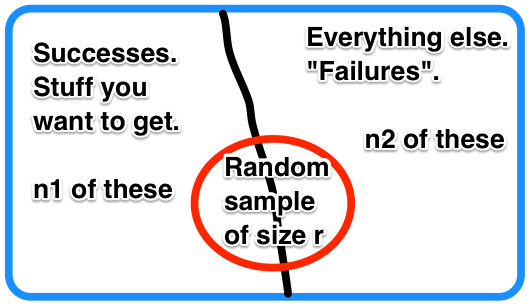
\includegraphics[width=\linewidth]{images/HypergeometricBucket.png}
\end{image}%
%
\par
\begin{theorem}{Hypergeometric Probability Function.}{}{x:theorem:HypergeometricPF}%
For a Hypergeometric random variable with \(R\) = \textbraceleft{}0, 1, ..., r\textbraceright{} and assuming \(n_1 \ge r\) and \(n-n_1 \ge r\),%
\begin{equation*}
f(x) = \frac{\binom{n_1}{x} \binom{n-n_1}{r-x}}{\binom{n}{r}}
\end{equation*}
%
\end{theorem}
\begin{proof}{}{g:proof:idp268}
For the following, we will presume thatSince you are sampling without replacement and trying only measure the number of items from your desired group in the sample, then the space of X will include R = \textbraceleft{}0, 1, ..., r\textbraceright{} assuming \(n_1 \ge r\) and \(n-n_1 \ge r\). In the case when r is too large for either of these, the formulas below will follow noting that binomial coefficients are zero if the top is smaller than the bottom or if the bottom is negative.%
\par
So f(x) = P(X = x) = P(x from the sample are from the target group and the remainder are not). Breaking these up gives%
\begin{equation*}
f(x) = \frac{\binom{n_1}{x} \binom{n-n_1}{r-x}}{\binom{n}{r}}\qedhere
\end{equation*}
%
\end{proof}
%
\par
For example, suppose that you have a bag of assorted candies but you really prefer the little dark chocolate bars. Because you are obsessive, you first empty the whole bag onto your desk and discover that the bag contains 33 equally-sized candy bars of which 6 of them are your delightful dark chocolate bars. Putting the bars randomly back into the bag, you find that a friend's friend's friend walks into the room and grabs a handful of 5 candy bars from your bag. You are shocked and would like to know the probability that this person got 2 or more of your dark chocolate candy bars.%
\par
As a good prob\slash{}stats student you recognize that this situation fits the requirements of the hypergeometric distribution with \(n_1 = 6, n_2 = 27, r=5\) and you want \(P(X \ge 2)\).  You determine that it would be easier to compute the complement%
\begin{equation*}
1 - P(X \le 1) = 1 - f(0) - f(1).
\end{equation*}
Therefore,%
\begin{equation*}
P (X \ge 2) = 1 - \frac{\binom{6}{0} \binom{27}{5}}{\binom{33}{5}} - \frac{\binom{6}{1} \binom{27}{4}}{\binom{33}{5}}
\end{equation*}
or after some simplification%
\begin{equation*}
P (X \ge 2) = 1 - \frac{13455}{39556} - \frac{8775}{19778} \approx 0.21617
\end{equation*}
Therefore, you have about 1 chance out of 5 that the friend got 2 or more of your bars. You can be somewhat confident that plenty of dark chocolate bars remain hoarded for yourself.%
\begin{theorem}{Properties of the Hypergeometric Distribution.}{}{x:theorem:HypergeometricProperties}%
%
\begin{enumerate}
\item{}\(f(x) = \frac{\binom{n_1}{x} \binom{n-n_1}{r-x}}{\binom{n}{r}}\) satisfies the properties of a probability function.%
\item{}\(\displaystyle \mu = r \frac{n_1}{n}\)%
\item{}\(\displaystyle \sigma^2 = r \frac{n_1}{n} \frac{n_2}{n} \frac{n-r}{n-1}\)%
\item{}\(\displaystyle \gamma_1 = \frac{(n - 2 n_1)\sqrt{n-1}(n - 2r)}{r n_1 (n - n_1) \sqrt{n-r}(n-2)}\)%
\item{}\(\gamma_2 = \) very complicated!%
\end{enumerate}
%
\end{theorem}
\begin{proof}{}{g:proof:idp269}
%
\begin{enumerate}
\item{}%
\begin{align*}
\sum_{x=0}^n \binom{n}{x} y^x & = (1+y)^n, \text{ by the Binomial Theorem}\\
& = (1+y)^{n_1} \cdot (1+y)^{n_2} \\
& = \sum_{x=0}^{n_1} \binom{n_1}{x} y^x \cdot \sum_{x=0}^{n_2} \binom{n_2}{x} y^x \\
& = \sum_{x=0}^n \sum_{t=0}^r \binom{n_1}{r} \binom{n_2}{r-t} y^x
\end{align*}
Equating like coefficients for the various powers of y gives%
\begin{equation*}
\binom{n}{r} = \sum_{t=0}^r \binom{n_1}{r} \binom{n_2}{r-t}.
\end{equation*}
Dividing gives%
\begin{equation*}
1 = \sum_{x=0}^r f(x).
\end{equation*}
%
\item{}For the mean%
\begin{align*}
\sum_{x=0}^n x \frac{\binom{n_1}{x} \binom{n-n_1}{r-x}}{\binom{n}{r}} & = 
\frac{1}{\binom{n}{r}} \sum_{x=1}^n  \frac{n_1(n_1-1)!}{(x-1)!(n_1-x)!}  \binom{n-n_1}{r-x}\\
& = \frac{n_1}{\binom{n}{r}} \sum_{x=1}^n  \frac{(n_1-1)!}{(x-1)!((n_1-1)-(x-1))!}  \binom{n-n_1}{r-x} \\
& = \frac{n_1}{\frac{n(n-1)!}{r!(n-r)!}} \sum_{x=1}^n  \binom{n_1-1}{x-1}  \binom{n-n_1}{r-x} 
\end{align*}
Consider the following change of variables for the summation:%
\begin{gather*}
y = x-1\\
n_3 = n_1-1\\
s = r-1\\
m = n-1
\end{gather*}
Then, this becomes%
\begin{align*}
\mu = \sum_{x=0}^n x \frac{\binom{n_1}{x} \binom{n-n_1}{r-x}}{\binom{n}{r}} & = r \frac{n_1}{n} \sum_{y=0}^m  \frac{\binom{n_3}{y} \binom{m-n_3}{s-y}}{\binom{m}{s}}\\
& = r \frac{n_1}{n} \cdot 1
\end{align*}
noting that the summation is in the same form as was show yields 1 above.%
\item{}For variance, we will use an alternate form of the definition that is useful when looking for cancellation options with the numerous factorials in the \hyperref[x:section:HypergeometricDistribution]{hypergeometric probability function~{\xreffont\ref{x:section:HypergeometricDistribution}}}.  Indeed, you can easily notice that%
\begin{equation*}
\sigma^2 = E[X^2] - \mu^2 = E[X^2-X]+E[X] -\mu^2 = E[X(X-1)] + \mu - \mu^2.
\end{equation*}
Since we have \(\mu = r \frac{n_1}{n}\) from above then let's focus on the first term only and use the substitutions%
\begin{gather*}
y = x-2\\
n_3 = n_1-2\\
s = r-2\\
m = n-2
\end{gather*}
%
\par
to get%
\begin{gather*}
E[X(X-1)] = \sum_{x=0}^n x(x-1) \frac{\binom{n_1}{x} \binom{n-n_1}{r-x}}{\binom{n}{r}}\\
= \sum_{x=2}^n x(x-1) \frac{\frac{n_1!}{x(x-1)(x-2)!(n_1-x)! } \binom{n-n_1}{r-x}}{\binom{n}{r}}\\
= \sum_{x=2}^n \frac{\frac{n_1!}{(x-2)!(n_1-x)! } \frac{n_2!}{(r-x)!(n_2-r+x)!}}{\binom{n}{r}}\\
= n_1 \cdot (n_1-1) \cdot  
\sum_{x=2}^n \frac{\frac{(n_3)!}{(x-2)!(n_3 -(x-2))! } \frac{n_2!}{((r-2)-(x-2))!(n_2-(r-2)+(x-2))!}}{\binom{n}{r}}\\
= n_1 \cdot (n_1-1) \sum_{y=0}^{m} \frac{\frac{(n_3)!}{y!(n_3 -y)! } \frac{n_2!}{(s-y)!(n_2-s+y)!}}{\binom{n}{r}}\\
= \frac{n_1 \cdot (n_1-1) \cdot r \cdot (r-1)}{n (n-1)} \sum_{y=0}^{m} \frac{\binom{(n_3)}{y} \binom{n_2}{s-y}}{\binom{m}{s}}\\
= \frac{n_1 \cdot (n_1-1) \cdot r \cdot (r-1)}{n (n-1)} 
\end{gather*}
where we have used the summation formula above that showed that f(x) was a probability function.%
\par
Putting this together with the earlier formula gives%
\begin{equation*}
\sigma^2 = \frac{n_1 \cdot (n_1-1) \cdot r \cdot (r-1)}{n (n-1)} + r \frac{n_1}{n} - \left ( r \frac{n_1}{n} \right )^2.
\end{equation*}
%
\item{}The formula and resulting proof of kurtosis is even more messy and we won’t bother with proving it for this distribution! If you start searching on the web for the formula then you will find many places just ignore the kurtosis for the hypergeometric.  So we will as well here and just note that as the parameters increase the resulting graph sure looks bell-shaped.  That is, approaching a kurtosis of 3.%
\end{enumerate}
%
\end{proof}
Occasionally in this text, we will use symbolic computational tools to create formulas. Indeed, many of the formulas presented in this text for some theorems and for many of the examples were created actually by using the open-source software Sage.  Sometimes Sage can figure things out for us and save you a lot of tedious computational time. Sometimes it can uncover things that you might not be able to manage the complicated derivations. And sometimes it works great. Below, Sage attempts to create the formulas presented above for the hypergeometric distribution and this time it can't figure things out.  Just for the fun of it we can still make the attempt...%
\begin{sageinput}
var('x,n,n1,r,m')

assume(x,'integer')
assume(n,'integer')
assume(n1,'integer')
assume(r,'integer')
assume(r<n1)

f = factorial(n1)/(factorial(x)*factorial(n1-x))*factorial(n-n1)/(factorial(r-x)*factorial(n-n1-r+x))*(factorial(r)*factorial(n-r))/factorial(n)

f(x=2)
mu = sum(x*f,x,0,r)
M2 = sum(x^2*f,x,0,r)
M3 = sum(x^3*f,x,0,r)
M4 = sum(x^4*f,x,0,r)

pretty_print('Mean = ',mu)

v = (M2-mu^2).factor()
pretty_print('Variance = ',v)
stand = sqrt(v)

sk = ((M3 - 3*M2*mu + 2*mu^3)).factor()/stand^3
pretty_print('Skewness = ',sk)

kurt = (M4 - 4*M3*mu + 6*M2*mu^2 -3*mu^4).factor()/stand^4
pretty_print('Kurtosis = ',(kurt-3).factor(),'+3')
\end{sageinput}
So, trying to prove the limiting result also doesn't work using the symbolic software.  To empirically demonstrate the conclusion then consider the following interactive cell where you can pick a starting point for \(n_1, n_1,\) and \(r\) and then by increasing k watch what happens.  You should notice that pretty soon the resulting hypergeometric distribution looks very much like a symmetric bell-shapped distribution.%
\begin{sageinput}
k = 30    # make this number larger and larger to see the limiting distribution with similar proportions
N1 = k*10      # desirable items
N2 = k*16      # the others
n = N1+N2
r = k*5        # sample size extracted without replacement from a random sample of all n

X = 0:r        # the space R of the random variable 
mu = r*N1/n      # the formula for mean of the Binomial Distributions
sdev = sqrt(mu*(N2/n)*(n-r)/(n-1))  # the formula for the standard deviation
sink("message")
dhyper( X, N1, N2, r )   # let's print out a bunch of actual probs
Phyper = dhyper(X, N1, N2, r )  # create the probability function over X
Psample = rhyper(10^6, N1, N2, r)  # to create a histogram, sample a lot

Xtop=max(Psample)          # for scaling the x-axis. Shift by 1/2 below.
hist(Psample, prob=TRUE, br=(-1:Xtop)+0.5, col="skyblue2", xlab="X", 
  main="Hypergeometric Probability Function vs Approximating 'Bell Curve'")
points(X, Phyper, pch=19, col="darkgreen")  # to create actual (x,f(x))

invisible(Pnormal <- function(X){dnorm(X, mean=mu, sd=sdev)})   # to overlap a bell curve
invisible(curve(Pnormal, col="red", lwd=2, add=TRUE))
\end{sageinput}
Note, if r=1 then you are back at a regular discrete uniform model. Indeed,%
\begin{equation*}
P(\text{desired item}) = 1 \cdot \frac{n_1}{n} = \mu .
\end{equation*}
which is indeed what you might expect when selecting once.%
\par
For many of the distributions to be discussed in this text, it appears that as parameters are allowed to increase the resulting distribution becomes more and more symmetrical and more and more bell-shaped. This is indeed the case for the hypergeometric distribution.  In general, you can check by seeing what happens to the skewness \(\gamma_1\) and the kurtosis \(\gamma_2\) and to see if \(\gamma_1 \rightarrow 0\) and \(\gamma_2 \rightarrow 3\).  If so, that is the definition for what is meant when a distribution is bell-shaped. Eventually, we will see that the "Normal Distribution" is the eventual model of a distribution that is always bell-shaped.%
\begin{theorem}{Hypergeometric Limiting Distribution.}{}{x:theorem:LimitingHypergeometric}%
For the \hyperref[x:theorem:HypergeometricPF]{hypergeometric distribution~{\xreffont\ref{x:theorem:HypergeometricPF}}}, as \(m \rightarrow \infty\)%
\begin{equation*}
\gamma_1 \rightarrow 0
\end{equation*}
and%
\begin{equation*}
\gamma_2 \rightarrow 3.
\end{equation*}
%
\end{theorem}
\begin{proof}{}{g:proof:idp270}
For skewness, take the limit of the skewness result above as \(n_1, n_2\), and \(r\) are uniformly increased together (i.e. all are doubled, tripled, etc.) To model this behavior one can simply scale each of those term by some variable \(k\) and then let \(k\) increase. Asymptotically, the result is%
\begin{equation*}
\lim_{k \rightarrow \infty} \frac{(nk-2n_1k)(nk-1)^{1/2}(nk-2rk)}{rkn_1k(nk-n_1k)(nk-rk)^{1/2}(nk-2)} ~ \lim_{k \rightarrow \infty} C \frac{k^{5/2}}{k^{9/2}}= 0.
\end{equation*}
%
\par
Similarly for kurtosis.  However, since we can't find a nice formula for the kurtosis then taking the limit can be difficult.  So, we will have to appeal to general results proved in a course that would follow up this one that would prove this fact must be true. Sadly, not here.%
\end{proof}
\leavevmode%
\begin{sageinput}
N1 = 10
N2 = 16
n = N1+N2
r = 5

X = 0:r        # the space R of the random variable 
mu = r*N1/n      # the formula for mean of the Binomial Distributions
sdev = sqrt(mu*(N2/n)*(n-r)/(n-1))  # the formula for the standard deviation
dhyper( X, N1, N2, r )   # let's print out a bunch of actual probs

Phyper = dhyper(X, N1, N2, r )  # create the probability function over X

Psample = rhyper(10^6, N1, N2, r)  # to create a histogram, sample a lot
Xtop=max(Psample)          # for scaling the x-axis. Shift by 1/2 below.
hist(Psample, prob=TRUE, br=(-1:Xtop)+0.5, col="skyblue2", xlab="X", 
  main="Hypergeometric Probability Function vs Approximating 'Bell Curve'")

points(X, Phyper, pch=19, col="darkgreen")  # to create actual (x,f(x))

Pnormal <- function(X){dnorm(X, mean=mu, sd=sdev)}   # to overlap a bell curve
curve(Pnormal, col="red", lwd=2, add=TRUE)
\end{sageinput}
%
\par
Consider the \hyperref[x:section:HypergeometricDistribution]{Hypergeometric Distribution~{\xreffont\ref{x:section:HypergeometricDistribution}}} for various values of \(n_1, n_2,\) and r using the interactive cell above. Notice what happens when you start with relatively small values of \(n_1, n_2,\) and r (say, start with \(n_1 = 5, n_2 = 8,\) and r = 4 and then doubling then all again and again. Consider the likely skewness and kurtosis of the graph as the values get larger.%
\par
In the interactive cell below, notice how many items are in each portion of the "Venn Bucket" when you change the size of the number extracted-{}-{}denoted by what is inside the circle.%
\begin{sageinput}
# Hypergeometric distribution over 0 .. N
# Size of classes N1 and N2 must be given as well as subset size r
var('x')
@interact(layout=dict(top=[['N1','N2','r']]))
def _(N1=input_box(10,width=5,label='$$ N_1 $$'),
    N2=input_box(10,width=5,label='$$ N_2 $$'),
    r=input_box(5,width=5,label='$$ r $$')):
    N = N1 + N2
    f = binomial(N1,x)*binomial(N2,r-x)/binomial(N,r)
    @interact
    def __(X = slider(0,min(r,N1),1)):
        Px = f(x=X)
        Pxapprox = Px.n(digits=8)
        formula = "\\frac{\\binom{%s}"%str(N1)+"{%s}"%str(X)+" \\binom{%s}"%str(N2)+"{%s}}"%str(r-X)+"{ \\binom{%s}"%str(N)+"{%s}}"%str(r)
        pretty_print(html("P(X = %s"%str(X)+") = $ %s $"%str(formula)+" = $ %s $"%str(latex(Px))+"$ \\approx %s $"%str(Pxapprox)))
        G = polygon([(0,0), (1,0), (1.2,1), (-.2,1)],color='lightblue')
        G += line([(0.5,0),(0.5,1)],thickness=2)
        G += circle((0.5,0.3),0.25,fill=True,facecolor='yellow',alpha=0.5,zorder=2)
        G += text("Things I want",(0.2,0.9))+text("Everything else",(0.8,0.9))
        G += text("%s"%X,(0.4,0.3),fontsize=30) + text("%s"%(r-X),(0.6,0.3),fontsize=30)
        G += text("%s"%(N1-X),(0.1,0.5),fontsize=30) + text("%s"%(N2-(r-X)),(0.9,0.5),fontsize=30)
        show(G, axes=0, figsize=(4,4) )
\end{sageinput}
\end{sectionptx}
%
%
\typeout{************************************************}
\typeout{Section 6.5 Generating Functions for Uniform-based Distributions}
\typeout{************************************************}
%
\begin{sectionptx}{Generating Functions for Uniform-based Distributions}{}{Generating Functions for Uniform-based Distributions}{}{}{x:section:EquallyLikelyGeneratingFunctions}
\hyperref[x:definition:DefnMomentGeneratingFunction]{Moment Generating Functions~{\xreffont\ref{x:definition:DefnMomentGeneratingFunction}}} can be derived for each of the distributions in this chapter.%
\begin{theorem}{Moment Generating Function for Discrete Uniform.}{}{x:theorem:MGFDiscrete}%
For a discrete random variable X on the space \(R\) = \textbraceleft{}1, 2, ..., n\textbraceright{},%
\begin{equation*}
M(t) = \frac{1}{n} \cdot \left [ e^t + e^{2t} + ... e^{nt} \right ] 
\end{equation*}
%
\end{theorem}
\begin{proof}{}{g:proof:idp271}
Presuming \(R\) = \textbraceleft{}1, 2, ..., n\textbraceright{},%
\begin{equation*}
M(t) = \sum_{x=1}^n e^{tx}/n = \frac{1}{n} \cdot \left [ e^t + e^{2t} + ... e^{nt} \right ] \qedhere
\end{equation*}
%
\end{proof}
\begin{theorem}{Moment Generating Function for Continuous Uniform.}{}{x:theorem:MGFContinuous}%
For a continuous random variable X on the space \(R = [a,b]\),%
\begin{equation*}
M(t) = \frac{e^{bx} - e^{ax}}{b-a}
\end{equation*}
%
\end{theorem}
\begin{proof}{}{g:proof:idp272}
Presuming \(R\) = [a,b],%
\begin{equation*}
M(t) = \int_a^b e^{tx} \frac{1}{b-a} dx = \frac{1}{b-a} \frac{1}{t} e^{tx} \big |_a^b = \frac{e^{bx} - e^{ax}}{b-a}\qedhere
\end{equation*}
%
\end{proof}
\begin{theorem}{Moment Generating Function for Hypergeometric.}{}{x:theorem:MGFHypergeometric}%
For a hypergeometric random variable over the space \(R\) = \textbraceleft{}0, 1, ..., min(\(r,n_\))\textbraceright{}.%
\begin{equation*}
M(t) = \text{TBA}
\end{equation*}
%
\end{theorem}
\begin{proof}{}{g:proof:idp273}
%
\begin{align*}
M(t) & = \sum_{x=0}^{n_1} e^{tx} \frac{\binom{n_1}{x} \binom{n-n_1}{r-x}}{\binom{n}{r}}\\
& = \text{a mess...}\qedhere
\end{align*}
%
\end{proof}
\end{sectionptx}
%
%
\typeout{************************************************}
\typeout{Section 6.6 Summary}
\typeout{************************************************}
%
\begin{sectionptx}{Summary}{}{Summary}{}{}{x:section:EquallyLikelySummary}
Here is a summary of the major formulas from this chapter:%
\par
\hyperref[x:theorem:DiscreteUniformPF]{Discrete Uniform f(x)~{\xreffont\ref{x:theorem:DiscreteUniformPF}}}%
\par
\hyperref[x:theorem:DiscreteUniformProperties]{Discrete Uniform statistics~{\xreffont\ref{x:theorem:DiscreteUniformProperties}}}%
\par
\hyperref[x:theorem:ContinuousUniformPF]{Continuous Uniform f(x)~{\xreffont\ref{x:theorem:ContinuousUniformPF}}}%
\par
\hyperref[x:theorem:ContinuousUniformProperties]{Continuous Uniform statistics~{\xreffont\ref{x:theorem:ContinuousUniformProperties}}}%
\par
\hyperref[x:theorem:HypergeometricPF]{Hypergeometric f(x)~{\xreffont\ref{x:theorem:HypergeometricPF}}}%
\par
\hyperref[x:theorem:HypergeometricProperties]{Hypergeometric statistics~{\xreffont\ref{x:theorem:HypergeometricProperties}}}%
\end{sectionptx}
%
%
\typeout{************************************************}
\typeout{Section 6.7 Exercises}
\typeout{************************************************}
%
\begin{sectionptx}{Exercises}{}{Exercises}{}{}{x:section:EquallyLikelyExercises}
\begin{inlineexercise}{- The Proverbial Urn Problem.}{g:exercise:idp274}%
You have an urn with 10 marbles of which \(n_1 = 6\) are red and \(N_2 = 4\) are blue. You select randomly r = 3 of the marbles without replacement and let \(X\) represent the number of red marbles in your sample. With \(R\) = \textbraceleft{}0, 1, 2, 3\textbraceright{}, determine:%
\begin{itemize}[label=\textbullet]
\item{}f(x)%
\item{}P(2 of the 3 are red) = f(2)%
\item{}P(at most 2 of the 3 are red) = f(0) + f(1) + f(2)%
\end{itemize}
%
\par\smallskip%
\noindent\textbf{\blocktitlefont Hint}.\hypertarget{g:hint:idp275}{}\quad{}This is hypergeometric using%
\begin{equation*}
f(x) = \frac{\binom{6}{x} \binom{4}{3-x}}{\binom{10}{3}}.
\end{equation*}
%
\end{inlineexercise}%
\begin{inlineexercise}{- Playing Cards.}{g:exercise:idp276}%
You randomly select a hand of five cards without replacement from an ordinary deck of playing cards.%
\begin{itemize}[label=\textbullet]
\item{}Determine the probability that four of the five are spades.%
\item{}Determine the probability that three of the five are face cards (ie, Jacks, Queens, Kings).%
\end{itemize}
%
\par\smallskip%
\noindent\textbf{\blocktitlefont Hint}.\hypertarget{g:hint:idp277}{}\quad{}This exercise is actually two different hypergeometric distributions: the first is the 13 spades vs the 39 other cards and the second is the 12 face cards vs the 40 other cards.%
\par\smallskip%
\noindent\textbf{\blocktitlefont Solution}.\hypertarget{g:solution:idp278}{}\quad{}%
\begin{equation*}
\frac{\binom{13}{4} \binom{39}{1}}{\binom{52}{5}}
\end{equation*}
%
\begin{equation*}
\frac{\binom{12}{3} \binom{40}{2}}{\binom{52}{5}}
\end{equation*}
%
\end{inlineexercise}%
\begin{inlineexercise}{- Starting Seniors.}{g:exercise:idp279}%
You are picking an eleven member football starting team by picking randomly from a group with 15 seniors and 35 others. Determine:%
\begin{itemize}[label=\textbullet]
\item{}P(all seniors)%
\item{}P(exactly 6 seniors)%
\item{}the expected number of seniors on the team%
\item{}If your team has all seniors, explain whether someone could suggest that your decision on members was unfair%
\end{itemize}
%
\par\smallskip%
\noindent\textbf{\blocktitlefont Hint}.\hypertarget{g:hint:idp280}{}\quad{}This is a hypergeometric distribution with \(n_1 = 15, n_2 = 35, r = 11\).%
\end{inlineexercise}%
\begin{inlineexercise}{- Old Faithful.}{g:exercise:idp281}%
Ole Faithful geyser in Yellowstone National Park erupts every 91 minutes. You show up at some random time in the eruption cycle and your tour bus plans to stay for 25 minutes. Determine the likelihood that you will be able to see it erupt.  Express your answer by giving correct formulas for \(f(x)\) and \(F(x)\) and then determine the specific answer to this question.%
\par\smallskip%
\noindent\textbf{\blocktitlefont Hint}.\hypertarget{g:hint:idp282}{}\quad{}This is the continuous uniform distribution over \(R\) = [0, 91].%
\end{inlineexercise}%
\begin{inlineexercise}{- Uniform Scenarios.}{g:exercise:idp283}%
Explain how the following situations can be modeled using either a discrete or continuous uniform distribution by identifying the space \(R\) and the corresponding \(f(x)\) for each situation.%
\begin{itemize}[label=\textbullet]
\item{}The location on a prize wheel where the spun wheel will stop.%
\item{}Given a clock with only a minute hand, the current one second interval.%
\item{}The location on a automobile tire where the next puncture will occur.%
\end{itemize}
%
\end{inlineexercise}%
\begin{inlineexercise}{- Continuous Uniform on a different space.}{g:exercise:idp284}%
Determine an explicit formula for \(f(x)\) and the mean and variance for an continuous uniform distribution over \(R = [-2,3] \cup [5,6] \cup [9,15]\).%
\par\smallskip%
\noindent\textbf{\blocktitlefont Solution}.\hypertarget{g:solution:idp285}{}\quad{}Since you must have%
\begin{equation*}
\int_{x \in R} f(x) dx = 1
\end{equation*}
and since \(f(x)\) must be constant than all you must do is measure the accumulated width of the intervals in \(R\). This is 5 + 1 + 6 = 12 and so%
\begin{equation*}
f(x)=\left\{\begin{matrix}
\frac{1}{12}, & -2 \le x \le 3
\\ \frac{1}{12}, & 5 \le x \le 6
\\ \frac{1}{12}, & 9 \le x \le 15
\\ 0, & \text{otherwise}
\end{matrix}\right.
\end{equation*}
For the mean,%
\begin{align*}
\int_{x \in R} x \frac{1}{12} dx & = \int_{-2}^3 \frac{x}{12} dx + \int_5^6 \frac{x}{12} dx + \int_9^{15} \frac{x}{12} dx\\
& = \frac{9-4}{24} + \frac{36-25}{24} + \frac{225-81}{24}\\
& = \frac{5+11+144}{24} = \frac{160}{24} = \frac{20}{3}.
\end{align*}
For the variance,%
\begin{align*}
\int_{x \in R} x^2 \frac{1}{12} dx - \mu^2 & = \int_{-2}^3 \frac{x^2}{12} dx + \int_5^6 \frac{x^2}{12} dx + \int_9^{15} \frac{x^2}{12} dx - \mu^2\\
& = \frac{81+8}{36} + \frac{216-125}{36} + \frac{3375-729}{36} - \big ( \frac{20}{3} \big )^2\\
& = \frac{89+91+2646}{36} - \frac{400}{9} = \frac{2826-1600}{36} \\
& = \frac{1226}{36} \approx	34.055.
\end{align*}
%
\end{inlineexercise}%
\begin{inlineexercise}{- Louisiana Mega Millions Lottery.}{g:exercise:idp286}%
To play the Mega Millions Louisiana Lottery consists of picking five numbers from 1 to 75 and one yellow Mega Ball number from 1 through 15. (You can play up to five different sets of numbers on each playslip but we will just assume one play per ticket to keep things straight.) Each play costs \textdollar{}1 and you can pay an additional \textdollar{}1 to apply a "multiplier" which multiplies any non-Jackpot prize by the Multiplier number (2, 3, 4, or 5) randomly selected at the time of the drawing.%
\par
On October 10, 2016 the jackpots listed were%
\begin{itemize}[label=\textbullet]
\item{}Match 5 plus Mega ball = Jackpot of \textdollar{}49,000,000 with cash value of \textdollar{}32,600,000%
\item{}Match only 5 = \textdollar{}1,000,000%
\item{}Match 4 plus Mega ball = \textdollar{}5,000%
\item{}Match only 4 =\textdollar{}500%
\item{}Match 3 plus Mega ball = \textdollar{}50%
\item{}Match only 3 = \textdollar{}5%
\item{}Match 2 plus Mega ball = \textdollar{}5%
\item{}Match 1 plus Mega ball = \textdollar{}2%
\item{}Match only the Mega ball = \textdollar{}1%
\end{itemize}
%
\par
Verify the posted odds%
\begin{itemize}[label=\textbullet]
\item{}Match 5 plus Mega ball = 1 in 258,890,850%
\item{}Match only 5 = 1 in 18,492,204%
\item{}Match 4 plus Mega ball = 1 in 739,688%
\item{}Match only 4 = 1 in 52,835%
\item{}Match 3 plus Mega ball = 1 in 10,720%
\item{}Match only 3 = 1 in 766%
\item{}Match 2 plus Mega ball = 1 in 473%
\item{}Match 1 plus Mega ball = 1 in 56%
\item{}Match only the Mega ball = 1 in 21%
\end{itemize}
%
\par
Determine the expected payout for each ticket purchased. Also, determine what the Jackpot would need to be in order for the game to be considered "fair" with an expected value of zero.%
\par\smallskip%
\noindent\textbf{\blocktitlefont Solution}.\hypertarget{g:solution:idp287}{}\quad{}Throughout these calculations, you can presume that the first five numbers are selected independently from the Mega Ball number. However, the first five numbers are selected without replacement so computing probabilities with those does not allow for independence. This part is hypergeometric with the \(n_1 = 5\) numbers you selected being the "desired" numbers and the Lottery Commission picking a subset of size r = 5 from the 75 possible numbers.  So, your likelihood of matching all five would be%
\begin{equation*}
\frac{\binom{5}{5} \cdot \binom{70}{0}}{\binom{75}{5}} = \frac{1}{17259390}.
\end{equation*}
Multiplying this by the 1 chance in 15 that you also match the Mega Ball gives%
\begin{equation*}
P(\text{Match 5 plus Mega Ball}) = \frac{1}{17259390} \cdot \frac{1}{15} = \frac{1}{258,890,850}.
\end{equation*}
To match only 5 means you also MUST miss the Mega Ball which has probability 14\slash{}15 to give%
\begin{equation*}
\frac{1}{17259390} \cdot \frac{14}{15} = \frac{1}{17259390 \cdot \frac{15}{14}} \approx \frac{1}{18492204}.
\end{equation*}
Continue in this manner to determine the other odds.%
\par
For the expected earnings, first determine a value function corresponding to each outcome and apply the discrete expected value process. This gives%
\begin{align*}
& \$32600000 \cdot \frac{1}{258,890,850} + \$1000000 \cdot \frac{1}{18,492,204} \\
& + \$5000 \cdot \frac{1}{739,688} + \$500 \cdot \frac{1}{52,835}\\
& + \$50 \cdot \frac{1}{10,720} + \$5 \cdot \frac{1}{766} \\
& + \$5 \cdot \frac{1}{473} + \$2 \cdot \frac{1}{56} + \$1 \cdot \frac{1}{21}\\
& \approx \$0.3013.
\end{align*}
So, the expected payout is approximately 30 cents. Subtracting the cost of playing (\textdollar{}1) indicates that the average winnings per play of the Louisiana Lottery would be -70 cents. So, you would be better off to take, say, 50 cents and just give it to the local school system every time you consider playing this game rather than actually playing.%
\par
To determine the Jackpot A needed to make this a fair game means to solve the equation%
\begin{align*}
& A \cdot \frac{1}{258,890,850} + \$1000000 \cdot \frac{1}{18,492,204} \\
& + \$5000 \cdot \frac{1}{739,688} + \$500 \cdot \frac{1}{52,835}\\
& + \$50 \cdot \frac{1}{10,720} + \$5 \cdot \frac{1}{766} \\
& + \$5 \cdot \frac{1}{473} + \$2 \cdot \frac{1}{56} + \$1 \cdot \frac{1}{21}\\
& = 1
\end{align*}
for A.%
\par
Finally, to deal with the multiplier, note that all but the Jackpot payouts would be increased by the multiplier m where \(m \in \{1,2,3,4,5\}\).  For the cost of an extra \textdollar{}1 (total cost of \textdollar{}2 per bet) the expected payout increases as the multiplier increases but each of these decreases likelihood of winning that payout by a factor of 1\slash{}5.  In general, let x = 1, 2, ..., 9 indicate the various winning options in order listed above, f(x) the corresponding probabilities listed for each option, and  u(x) the listed payouts. Then the expected payout is given by%
\begin{equation*}
\$32600000 \cdot \frac{1}{258,890,850} + \sum_{m=1}^5
\sum_{x=2}^9 m \cdot u(x) f(x)/5 
\end{equation*}
or%
\begin{align*}
\$32600000 \cdot \frac{1}{258,890,850} & + \sum_{m=1}^5 \frac{m}{5} \sum_{x=2}^9 u(x) f(x) \\
& = \frac{\$32600000}{258890850} + \sum_{m=1}^5 \frac{m}{5} 0.17539\\
& = 0.12592 + 3 \cdot 0.17539\\
& = 0.65209
\end{align*}
Therefore, the expect value of spending another dollar to get the multiplier effect is about -\textdollar{}1.35.  Since this is slightly less than doubling the expected loss of 70 cents for playing without the multiplier with \textdollar{}1, it make more sense to bet \textdollar{}2 once rather than betting \textdollar{}1 twice.  Or, you can send the extra nickel to this author of this text and call it quits.%
\end{inlineexercise}%
\end{sectionptx}
\end{chapterptx}
%
%
\typeout{************************************************}
\typeout{Chapter 7 Distributions based upon Bernoulli Trials}
\typeout{************************************************}
%
\begin{chapterptx}{Distributions based upon Bernoulli Trials}{}{Distributions based upon Bernoulli Trials}{}{}{x:chapter:BernoulliBasedDistributions}
%
%
\typeout{************************************************}
\typeout{Section 7.1 Success vs Failure?}
\typeout{************************************************}
%
\begin{sectionptx}{Success vs Failure?}{}{Success vs Failure?}{}{}{x:section:BernoulliIntroduction}
Many practical problems involve measuring simply whether something was a success or a failure. In these situations, "success" should not be interpreted as having any moral or subjective meaning but only construed to mean that something you are looking for actually occurs.%
\par
In situation where a single trial is performed and the result is determined only to be a success or failure is called a Bernoulli event. Indeed, one could create a corresponding probability function using a random variable \(X\) over the space \(R = \{0, 1 \}\) mapping \(X\)(success) = 1 and \(X\)(Failure)=0. If p = P(Success) then%
\begin{equation*}
f(x) = p^x \cdot (1-p)^{1-x}
\end{equation*}
would be a formula but which only related to two values:%
\begin{equation*}
P(\text{Failure}) = f(0) = (1-p)
\end{equation*}
%
\begin{equation*}
P(\text{Success}) = f(1) = p
\end{equation*}
%
\par
Notice that p=0 means that you will always get a failure and that p=1 means that you will always get a success. In these cases, \(X\) would no longer be a random variable since the outcome for \(X\) could be predicted with certainty. Therefore, we will always assume that \(0 < p < 1\).%
\par
The Bernoulli distribution on its own is not extremely useful but serves as a starting point for several others that are useful.  Indeed, in this chapter you will investigate distributions that relate some number of successes in multiple trials to some number of independent trials. The difference between these distributions will be that one of these variables will be fixed and the other one will be variable.%
\par
In this chapter, you will investigate the following distributions:%
\begin{enumerate}
\item{}Binomial - the number of trials is fixed and \(X\) measures the variable number of successes%
\item{}Geometric - the number of successes is fixed-{}-{}at 1-{}-{}and \(X\) measures the variable number of trials%
\item{}Negative Binomial - the number of successes is fixed and \(X\) measures the variable number of trials%
\end{enumerate}
%
\end{sectionptx}
%
%
\typeout{************************************************}
\typeout{Section 7.2 Binomial Distribution}
\typeout{************************************************}
%
\begin{sectionptx}{Binomial Distribution}{}{Binomial Distribution}{}{}{x:section:BinomialDistribution}
Consider a sequence  of n independent Bernoulli trials with the likelihood of a success p on each individual trial stays constant from trial to trial with \(0 \lt p \lt 1 \). If we let the variable \(X\) measure the number of successes obtained when doing a fixed number of trials n with \(R = \{ 0, 1, ..., n \}\), then the resulting distribution of probabilities is called a Binomial Distribution.%
\par
Now, let's determine the actual probability function for this distribution.%
\par
\begin{theorem}{Derivation of Binomial Probability Function.}{}{x:theorem:BinomialProbabilityFunction}%
For R = \textbraceleft{}0, 1, ..., n\textbraceright{},%
\begin{equation*}
f(x) = \binom{n}{x}p^x(1-p)^{n-x}
\end{equation*}
%
\end{theorem}
\begin{proof}{}{g:proof:idp288}
Since successive trials are independent, then the probability of X successes occurring within n trials is given by%
\begin{equation*}
P(X=x) = \binom{n}{x}P(SS...SFF...F) = 		
\binom{n}{x}p^x(1-p)^{n-x}\qedhere
\end{equation*}
%
\end{proof}
%
\par
\begin{theorem}{Verification of Binomial Distribution Formula.}{}{g:theorem:idp289}%
%
\begin{equation*}
\sum_{x \in R} f(x) = \sum_{x=0}^n \binom{n}{x}p^x(1-p)^{n-x} = 1.
\end{equation*}
%
\end{theorem}
\begin{proof}{}{g:proof:idp290}
Using the Binomial Theorem with a = p and b = 1-p yields%
\begin{equation*}
\sum_{x=0}^n \binom{n}{x}p^x(1-p)^{n-x} = (p + (1-p))^n = 1\qedhere
\end{equation*}
%
\end{proof}
%
\par
The following interactive cell illustrates the range of choices for a Binomial setup with fixed N and fixed p:%
\par
\leavevmode%
\begin{sageinput}
# Binomial distribution over 0 .. N
# N and p need to be given
var('x')
@interact(layout=dict(top=[['N','p']]))
def _(N=input_box(10,width=5,label='$$ N $$'),
    p=input_box(3/10,width=5,label='$$ p $$')):
    f = binomial(N,x)*p^x*(1-p)^(N-x)
    @interact
    def __(X = slider(0,N,1)):
        Px = f(x=X)
        Pxapprox = Px.n(digits=8)
        formula = "\\binom{%s}"%str(N)+"{%s}"%str(X)+"({%s})"%str(p)+"^{%s}"%str(X)+"(1-{%s})"%str(p)+"^{%s}"%str(N-X)
        pretty_print(html("P(X = %s"%str(X)+") = $ %s $"%str(formula)+" = $ %s $"%str(latex(Px))+"$ \\approx %s $"%str(Pxapprox)))
        G = polygon([(0,0), (1,0), (1,1), (0,1)],thickness=10,color='blue',alpha=0.7,zorder=1)

        if X > 0:
            R =[j for j in range(N)] 
            selected = sample(R, X)
            for k in selected:
                xk = sqrt(k)*cos(k)/N^(4/5)+0.5
                yk = sqrt(k)*sin(k)/N^(4/5)+0.5
                G += circle((xk,yk),0.05,fill=True,facecolor='red',zorder=3) 
                G += text('p',(xk,yk))

        for k in range(N):
            xk = sqrt(k)*cos(k)/N^(4/5)+0.5
            yk = sqrt(k)*sin(k)/N^(4/5)+0.5
            G += circle((xk,yk),0.05,zorder=2,fill=True, facecolor="white")
   
        show(G, axes=0, figsize=(4,4) )
\end{sageinput}
%
\begin{example}{Flipping a coin a fixed number of times.}{g:example:idp291}%
Let's consider a simple example for flipping coins. Indeed, suppose you flip a coin exactly 20 times and need to determine the probability of getting exactly 10 heads.%
\par
This is binomial with n = 20, p = 1\slash{}2 and you are looking for f(10). With these values%
\begin{equation*}
f(10) = \binom{20}{10} \cdot \left ( \frac{1}{2} \right )^{10} \cdot \left ( \frac{1}{2} \right 	)^{20-10} = \frac{46189}{262144} \approx 0.176
\end{equation*}
Note that the mean for this distribution is also 10 so one might expect 10 heads in general%
\par
If you rather would prefer to determine the probability of getting 10 or fewer heads requires F(10) = f(0) + f(1) + ... + f(10). There is no "nice" formula for F but this calculation can be performed using a graphing calculator, such as the TI-84 with F(x) = binomcdf(n,p,x). In this case, F(10) = binomcdf(20,1\slash{}2,10) = 0.588.%
\end{example}
\begin{inlineexercise}{WebWork - Binomial.}{g:exercise:idp292}%
A coin is tossed 11 times.%
\par
a) How many different outcomes are possible?  \fillin{9.090909090909092}%
\par
b) What is the probability of getting exactly 4 heads? \fillin{9.090909090909092}%
\par
c) What is the probability of getting at least 2 heads? \fillin{9.090909090909092}%
\par
d) What is the probability of getting at most 7 heads? \fillin{9.090909090909092}%
\par\smallskip%
\noindent\textbf{\blocktitlefont Answer 1}.\hypertarget{g:answer:idp293}{}\quad{}\(2048\)%
\par\smallskip%
\noindent\textbf{\blocktitlefont Answer 2}.\hypertarget{g:answer:idp294}{}\quad{}\(0.1611328125\)%
\par\smallskip%
\noindent\textbf{\blocktitlefont Answer 3}.\hypertarget{g:answer:idp295}{}\quad{}\(0.994140625\)%
\par\smallskip%
\noindent\textbf{\blocktitlefont Answer 4}.\hypertarget{g:answer:idp296}{}\quad{}\(0.88671875\)%
\end{inlineexercise}%
\begin{example}{Testing critical components.}{g:example:idp297}%
Often one will test a critical system components for failure and toward that end collect a sample of 100 of these components from the manufacturer. Suppose the component is listed as having a p = 0.01 probability of breaking and you want to know the likelihood that at most 1 of the tested components actually fails when tested. You find it reasonable to presume that different components succeed or fail independently of each other. So, you can model this situation with a binomial distribution.%
\par
If \(X\) measures the number of components that fail when tested, the specific probability function is given by%
\begin{equation*}
f(x) = \binom{100}{x} 0.01^x 0.99^{100-x}.
\end{equation*}
The probability that at most one component fails is then given by%
\begin{equation*}
F(1) = f(0) + f(1) = \binom{100}{0} 0.01^0 0.99^{100} + \binom{100}{1} 0.01^1 0.99^99 \\ = 0.99^{100} + 100 \cdot 0.01 \cdot 0.99^{99} = 0.99^{99}(0.99 + 100 \cdot 0.01 \\ = 0.99^{99} \cdot 1.99 \approx 0.73576.
\end{equation*}
%
\end{example}
Utilize the interactive cell below to compute \(f(x)\) and \(F(x)\) for the Binomial distribution%
\par
\leavevmode%
\begin{sageinput}
# Binomial calculator
@interact
def _(p=input_box(3/10,width=15),n=input_box(10,width=15)):
    R = range(n+1)
    f(x) = binomial(n,x)*p^x*(1-p)^(n-x)
    acc = 0
    pretty_print("Binomial Calculator")
    for k in R:
        prob = f(x=k)
        acc = acc+prob
        pretty_print('f(%s) = '%k,' %.8f'%prob,' and F(%s) = '%k,' %.8f'%acc)
\end{sageinput}
%
\par
\begin{theorem}{Binomial Distribution Statistics.}{}{x:theorem:BinomialStatistics}%
%
\begin{equation*}
\mu = np
\end{equation*}
%
\begin{equation*}
\sigma^2 = np(1-p)
\end{equation*}
%
\begin{equation*}
\gamma_1 = \frac{1-2p}{\sqrt{np(1-p)}}
\end{equation*}
%
\begin{equation*}
\gamma_2 = \frac{1-6p(1-p)}{np(1-p)} + 3
\end{equation*}
%
\end{theorem}
\begin{proof}{}{g:proof:idp298}
For the \hyperlink{x:li:TheoreticalMean}{mean~{\xreffont 1}},%
\begin{align*}
\mu & = E[X] \\
& = \sum_{x=0}^{n} {x \binom{n}{x} p^x (1-p)^{n-x}}\\
& = \sum_{x=1}^{n} {x \frac{n(n-1)!}{x(x-1)!(n-x)!} p^x (1-p)^{n-x}}\\
& = np \sum_{x=1}^{n} {\frac{(n-1)!}{(x-1)!((n-1)-(x-1))!} p^{x-1} (1-p)^{(n-1)-(x-1)}}
\end{align*}
Using the change of variables \(k=x-1\) and \(m = n-1\) yields a binomial series%
\begin{align*}
& = np \sum_{k=0}^{m} {\frac{m!}{k!(m-k)!} p^k (1-p)^{m-k}}\\
& = np (p + (1-p))^m = np
\end{align*}
%
\par
For the \hyperlink{x:li:TheoreticalVariance}{variance~{\xreffont 2}},%
\begin{gather*}
\sigma^2  = E[X(X-1)] + \mu - \mu^2 \\
= \sum_{x=0}^{n} {x(x-1) \binom{n}{x} p^x (1-p)^{n-x}} + np - n^2p^2\\
= \sum_{x=2}^{n} {x(x-1) \frac{n(n-1)(n-2)!}{x(x-1)(x-2)!(n-x)!} p^x (1-p)^{n-x}}  + np - n^2p^2\\
= n(n-1)p^2 \sum_{x=2}^{n} {\frac{(n-2)!}{(x-2)!((n-2)-(x-2))!} p^{x-2} (1-p)^{(n-2)-(x-2)}} + np - n^2p^2
\end{gather*}
%
\par
Using the change of variables \(k=x-2\) and \(m = n-2\) yields a binomial series%
\begin{gather*}
= n(n-1)p^2  \sum_{k=0}^{m} {\frac{m!}{k!(m-k)!} p^k (1-p)^{m-k}} + np - n^2p^2\\
= n(n-1)p^2 + np - n^2p^2 = np - np^2 = np(1-p)
\end{gather*}
%
\par
The \hyperlink{x:li:TheoreticalSkewness}{skewness~{\xreffont 3}} and \hyperlink{x:li:TheoreticalKurtosis}{kurtosis~{\xreffont 4}} can be found similarly using formulas involving E[X(X-1)(X-2)] and E[X(X-1)(X-2)(X-3)]. The complete determination is performed using Sage below.%
\end{proof}
%
\par
The following uses Sage to symbolically confirm the general formulas for the Binomial distribution.%
\par
\leavevmode%
\begin{sageinput}
var('x,n,p')
assume(x,'integer')
f(x) = binomial(n,x)*p^x*(1-p)^(n-x)
mu = sum(x*f,x,0,n)
M2 = sum(x^2*f,x,0,n)
M3 = sum(x^3*f,x,0,n)
M4 = sum(x^4*f,x,0,n)

pretty_print('Mean = ',mu)

v = (M2-mu^2).factor()
pretty_print('Variance = ',v)
stand = sqrt(v)

sk = ((M3 - 3*M2*mu + 2*mu^3)).factor()/stand^3
pretty_print('Skewness = ',sk)

kurt = (M4 - 4*M3*mu + 6*M2*mu^2 -3*mu^4).factor()/stand^4
pretty_print('Kurtosis = ',(kurt-3).factor(),'+3')
\end{sageinput}
%
 Once again, you can see that as one of the parameters is allowed to increase without bound this distribution must become symmetrical and bell-shaped. \begin{theorem}{Binomial Limiting Distribution.}{}{x:theorem:LimitingBinomial}%
For the \hyperref[x:theorem:BinomialProbabilityFunction]{binomial distribution~{\xreffont\ref{x:theorem:BinomialProbabilityFunction}}}, as \(m \rightarrow \infty\)%
\begin{equation*}
\gamma_1 \rightarrow 0
\end{equation*}
and%
\begin{equation*}
\gamma_2 \rightarrow 3.
\end{equation*}
%
\end{theorem}
\begin{proof}{}{g:proof:idp299}
For skewness, take the limit of the skewness result above%
\begin{equation*}
\lim_{n \rightarrow \infty} \frac{n(2p-1)(p-1)p}{(-n(p-1)p)^{3/2}} = \lim_{n \rightarrow \infty} C \frac{n}{n^{3/2}} = 0.
\end{equation*}
%
\par
Similarly for kurtosis%
\begin{equation*}
\lim_{n \rightarrow \infty} -\frac{6p^2 - 6p + 1}{n (p - 1) p} +3 = 0 + 3 = 3.\qedhere
\end{equation*}
%
\end{proof}
\begin{inlineexercise}{WebWork - Binomial.}{g:exercise:idp300}%
The Census Bureau reports that 82\% of Americans over the age of 25 are high school graduates. A survey of randomly selected residents of certain county included 1260 who were over the age of 25, and 1086 of them were high school graduates.%
\par
(a) \(\) Find the mean and standard deviation for the number of high school graduates in groups of 1260 Americans over the age of 25.%
\par
Mean = \fillin{6.818181818181818}%
\par
Standard deviation = \fillin{6.818181818181818}%
\par
(b) \(\) Is that county result of 1086 unusually high, or low, or neither?%
\par
(Enter HIGH or LOW or NEITHER) \fillin{6.818181818181818}%
\par\smallskip%
\noindent\textbf{\blocktitlefont Answer 1}.\hypertarget{g:answer:idp301}{}\quad{}\(1033.2\)%
\par\smallskip%
\noindent\textbf{\blocktitlefont Answer 2}.\hypertarget{g:answer:idp302}{}\quad{}\(13.6373017859106\)%
\par\smallskip%
\noindent\textbf{\blocktitlefont Answer 3}.\hypertarget{g:answer:idp303}{}\quad{}high%
\end{inlineexercise}%
\leavevmode%
\begin{sageinput}
n = 10
p = 0.3
X = 0:n    # the space R of the random variable 
mu = n*p      # the formula for mean of the Binomial Distributions
sdev = sqrt(n*p*(1-p))  # the formula for the standard deviation
if(n < 101){
dbinom( X, n, p )   # let's print out a bunch of actual probs if N reasonable
}

Pbinom = dbinom(X, n, p )  # create the probability function over X

Psample = rbinom(10^6, n, p)  # to create a histogram, sample a lot
Xtop=max(Psample)          # for scaling the x-axis. Shift by 1/2 below.
hist(Psample, prob=TRUE, br=(-1:Xtop)+0.5, col="skyblue2", xlab="X", 
  main="Binomial Probability Function vs Approximating 'Bell Curve'")

points(X, Pbinom, pch=19, col="darkgreen")  # to create actual (x,f(x))

Pnormal <- function(X){dnorm(X, mean=mu, sd=sdev)}   # to overlap a bell curve
curve(Pnormal, col="red", lwd=2, add=TRUE)
\end{sageinput}
%
\par
You can of course get specific values and graph the Binomial Distribution using R as well...%
\par
\leavevmode%
\begin{sageinput}
n <- 10
p <- 0.3

paste('Probability Function')
dbinom(0:n, n, p)   # gives the probability function
paste('Distribution function')
pbinom(0:n, n, p)   # gives the distribution function
paste('A random sample')
rbinom(15, n, p)    # gives a random sample of 15 items from b(n,p)

x <- dbinom(0:n, size=n, prob=p)
barplot(x,names.arg=0:n, main=sprintf(paste('n=',n,' and p= ',p)))
\end{sageinput}
%
\end{sectionptx}
%
%
\typeout{************************************************}
\typeout{Section 7.3 Geometric Distribution}
\typeout{************************************************}
%
\begin{sectionptx}{Geometric Distribution}{}{Geometric Distribution}{}{}{x:section:GeometricDistribution}
Consider the situation where one can observe a sequence  of independent trials where the likelihood of a success on each individual trial stays constant from trial to trial. Call this likelihood the probably of "success" and denote its value by \(p\) where \(0 \lt p \lt 1 \). If we let the variable \(X\) measure the number of trials needed in order to obtain the first success with \(R = \{1, 2, 3, ... \}\), then the resulting distribution of probabilities is called a Geometric Distribution.%
\par
\begin{theorem}{}{}{x:theorem:GeometricProbabilityFunction}%
For a Geometric variable \(X\) with \(R = \{1, 2, 3, ... \}\),%
\begin{equation*}
f(x) = (1-p)^{x-1} \cdot p
\end{equation*}
%
\end{theorem}
\begin{proof}{}{g:proof:idp304}
Since successive trials are independent, then the probability of the first success occurring on the mth trial presumes that the previous m-1 trials were all failures.  Therefore the desired probability is given by%
\begin{equation*}
f(x) = P(X = x) = P(FF...FS) = (1-p)^{x-1}p\qedhere
\end{equation*}
%
\end{proof}
%
\begin{example}{Flipping a die until getting a success.}{g:example:idp305}%
Let's consider a simple example for rolling a 24-sided die until you get a multiple of 9...that is, either a 9 or an 18. Successive rolls of a die would appear to be independent events and the probability of getting a 9 or 18 on any given roll is \(p = \frac{1}{12}\). What is then the likelihood that it takes more than three rolls in order for you to get your first success?%
\par
This is easily modeled by a geometric distribution and you are looking for%
\begin{equation*}
P(X > 3) = 1 - P(X \le 3) = 1 - F(3) = 1 - f(1) - f(2) - f(3) \\
1 - \frac{1}{12} - \frac{11}{12} \cdot \frac{1}{12} - (\frac{11}{12})^2 \frac{1}{12} \approx 0.77025.
\end{equation*}
%
\end{example}
\begin{example}{Testing a critical component until failure.}{g:example:idp306}%
Often one will test a critical system component until it fails to see how long the component works. Suppose you have a particular component that on any given trial has a p=0.01 probability of breaking. You also might find it reasonable to presume that succesive trials are independent which could be the case if the component shows no wear from trial to trial. So, you can model this situation with a geometric distribution and the probability that the component fails on the x-th trial is given by%
\begin{equation*}
f(x) = 0.99^{x-1} \cdot 0.01.
\end{equation*}
For some reason, you might be interested in whether the component fails on the 5th trial. The probability of this outcome is given by%
\begin{equation*}
f(5) = 0.99^4 \cdot 0.01 \approx 0.0096
\end{equation*}
so it is unlikely that the component will fail on exactly the 5th trial. However, what about failing on one of the first five trials? Then, you would need%
\begin{equation*}
F(5) = f(1)+f(2)+f(3)+f(4)+f(5) \\ = 0.01 + 0.99 \cdot 0.01 + 0.99^2 \cdot 0.01 + 0.99^3 \cdot 0.01 + 0.99^4 \cdot 0.01 \approx 0.049
\end{equation*}
which is still relatively small. Indeed, with such a small probability of failure, you might expect the component to last for some time. Indeed, we will uncover a formula below for the number of trials, on average, you might expect before failure.%
\end{example}
Let's go ahead and verify this probability function and investigate some of the geometric distribution's properties.%
\par
\begin{theorem}{Geometric Distribution sums to 1.}{}{g:theorem:idp307}%
%
\begin{equation*}
f(x) = (1-p)^{x-1}p
\end{equation*}
sums to 1 over \(R = \{ 1, 2, ... \}\)%
\end{theorem}
\begin{proof}{}{g:proof:idp308}
%
\begin{equation*}
\sum_{x=1}^{\infty} {f(x)} = \sum_{x=1}^{\infty} {(1-p)^{x-1} p} \\ = p \sum_{j=0}^{\infty} {(1-p)^j} = p \frac{1}{1-(1-p)} = 1
\end{equation*}
using a change of variables j = x-1 and the known value for the sum of the geometric series.%
\end{proof}
%
\par
\leavevmode%
\begin{sageinput}
# Geometric distribution over 0 .. n
# Probability of success on one independent trial = p must also be given
var('x')
# n = 50 by default. actually should be infinite
@interact
def _(p=input_box(1/10,label='p = ',width=10),n=[25,50,75,100,200]):
    np1 = n+1
    R = range(1,np1)
    f(x) = (1-p)^(x-1)*p
    F(x) = 1 - (1-p)^x
    pretty_print(html('Density Function: $f(x) =%s$'%str(latex(f(x)))+' over the space $R = %s$'%str(R)))
    points((k,f(x=k)) for k in R).show(title="Probability Function")
    print
    points((k,F(x=k)) for k in R).show(title="Distribution Function")
    if (n == 25):
        for k in R:
            pretty_print(html('$f(%s'%k+') = %s'%latex(f(x=k))+' \\approx %s$'%f(x=k).n(digits=5)))
\end{sageinput}
%
\par
\begin{theorem}{Geometric Statistics Theorem.}{}{x:theorem:GeometricStatistics}%
For the geometric distribution,%
\begin{equation*}
\mu = 1/p
\end{equation*}
%
\begin{equation*}
\sigma^2  = \frac{1-p}{p^2}
\end{equation*}
%
\begin{equation*}
\gamma_1 = \frac{2-p}{\sqrt{1-p}}
\end{equation*}
%
\begin{equation*}
\gamma_2 = \frac{p^2-6p+6}{1-p} + 3
\end{equation*}
%
\end{theorem}
\begin{proof}{}{g:proof:idp309}
For the \hyperlink{x:li:TheoreticalMean}{mean~{\xreffont 1}},%
\begin{align*}
\mu & = E[X] = \sum_{x=1}^{\infty} {x(1-p)^{x-1}p}\\
& = p \sum_{x=1}^{\infty} {x(1-p)^{x-1}}\\
& = p \frac{1}{(1-(1-p))^2}\\
& = p \frac{1}{p^2} = \frac{1}{p}
\end{align*}
%
\par
For the \hyperlink{x:li:TheoreticalVariance}{variance~{\xreffont 2}},%
\begin{align*}
\sigma^2 & = E[X(X-1)] + \mu - \mu^2 \\
& = \sum_{x=1}^{\infty} {x(x-1)(1-p)^{x-1}p} + \mu - \mu^2 \\
& = (1-p)p \sum_{x=2}^{\infty} {x(x-1)(1-p)^{x-2}} + \frac{1}{p} - \frac{1}{p^2}\\
& = (1-p)p \frac{2}{(1-(1-p))^3} + \frac{1}{p} - \frac{1}{p^2}\\
& = \frac{1-p}{p^2}\qedhere
\end{align*}
%
\end{proof}
%
\par
\begin{theorem}{Geometric Distribution Function.}{}{g:theorem:idp310}%
%
\begin{equation*}
F(x) =  1- (1-p)^{x}
\end{equation*}
%
\end{theorem}
\begin{proof}{}{g:proof:idp311}
Consider the accumulated probabilities over a range of values...%
\begin{align*}
P(X \le x) & = 1 - P(X \gt x)\\
& = 1- \sum_{k={x+1}}^{\infty} {(1-p)^{k-1}p}\\
& = 1- p \frac{(1-p)^{x}}{1-(1-p)}\\
& = 1- (1-p)^{x}\qedhere
\end{align*}
%
\end{proof}
%
\begin{theorem}{Statistics for Geometric Distribution.}{}{g:theorem:idp312}%
Mean, Variance, \hyperlink{x:li:TheoreticalSkewness}{Skewness~{\xreffont 3}}, \hyperlink{x:li:TheoreticalKurtosis}{Kurtosis~{\xreffont 4}} computed by Sage.%
\end{theorem}
\begin{proof}{}{g:proof:idp313}
See the interactive Sage cell below...%
\end{proof}
\begin{sageinput}
var('x,n,p')
assume(x,'integer')
f(x) = p*(1-p)^(x-1)
mu = sum(x*f,x,0,oo).full_simplify()
M2 = sum(x^2*f,x,0,oo).full_simplify()
M3 = sum(x^3*f,x,0,oo).full_simplify()
M4 = sum(x^4*f,x,0,oo).full_simplify()

pretty_print('Mean = ',mu)

v = (M2-mu^2).factor().full_simplify()
pretty_print('Variance = ',v)
stand = sqrt(v)

sk = (((M3 - 3*M2*mu + 2*mu^3))/stand^3).full_simplify()
pretty_print('Skewness = ',sk)

kurt = (M4 - 4*M3*mu + 6*M2*mu^2 -3*mu^4).factor()/stand^4
pretty_print('Kurtosis = ',(kurt-3).factor(),'+3')
\end{sageinput}
\begin{theorem}{The Geometric Distribution yields a memoryless model..}{}{x:theorem:TheoremGeometricMemoryless}%
If X has a geometric distribution and a and b are nonnegative integers, then%
\begin{equation*}
P( X > a + b | X > b ) = P( X > a)
\end{equation*}
%
\end{theorem}
\begin{proof}{}{g:proof:idp314}
Using the definition of conditional probability,%
\begin{align*}
P( X > a + b | X > b ) & = \frac{P( X > a + b \cap X > b )}{P( X > b)}\\
& = \frac{P( X > a + b )}{P( X > b)}\\
& = \frac{(1-p)^{a+b}}{(1-p)^b}\\
& = (1-p)^a\\
& = P(X > a)\qedhere
\end{align*}
%
\end{proof}
\end{sectionptx}
%
%
\typeout{************************************************}
\typeout{Section 7.4 Negative Binomial}
\typeout{************************************************}
%
\begin{sectionptx}{Negative Binomial}{}{Negative Binomial}{}{}{x:section:NegativeBinomial}
Consider the situation where one can observe a sequence  of independent trials where the likelihood of a success on each individual trial stays constant from trial to trial. Call this likelihood the probably of "success" and denote its value by \(p\) where \(0 \lt p \lt 1 \). If we let the variable \(X\) measure the number of trials needed in order to obtain the rth success, \(r \ge 1\), with \(R = \{r, r+1, r+2, ... \}\) then the resulting distribution of probabilities is called a Geometric Distribution.%
\par
Note that r=1 gives the Geometric Distribution.%
\par
\begin{theorem}{Negative Binomial Series.}{}{x:theorem:NegBinomSeries}%
%
\begin{equation*}
\displaystyle \frac{1}{(a+b)^n} = \sum_{k=0}^{\infty} {(-1)^k \binom{n + k - 1}{k} a^k b^{-n-k}}
\end{equation*}
%
\end{theorem}
\begin{proof}{}{g:proof:idp315}
First, convert the problem to a slightly different form: \(\frac{1}{(a+b)^n} = \frac{1}{b^n} \frac{1}{(\frac{a}{b}+1)^n} 
= \frac{1}{b^n} \sum_{k=0}^{\infty} {(-1)^k \binom{n + k - 1}{k} \left ( \frac{a}{b} \right ) ^k}\)%
\par
So, let's replace \(\frac{a}{b} = x\) and ignore for a while the term factored out. Then, we only need to show%
\begin{equation*}
\sum_{k=0}^{\infty} {(-1)^k \binom{n + k - 1}{k} x^k} = \left ( \frac{1}{1+x} \right )^n 
\end{equation*}
However%
\begin{align*}
\left ( \frac{1}{1+x} \right )^n & = \left ( \frac{1}{1 - (-x)} \right )^n \\
& = \left ( \sum_{k=0}^{\infty} {(-1)^k x^k} \right )^n
\end{align*}
%
\par
This infinite sum raised to a power can be expanded by distributing terms in the standard way. In doing so, the various powers of x multiplied together will create a series in powers of x involving \(x^0, x^1, x^2, ...\). To detemine the final coefficients notice that the number of time \(m^k\) will appear in this product depends upon the number of ways one can write k as a sum of nonnegative integers.%
\par
For example, the coefficient of \(x^3\) will come from the n ways of multiplying the coefficients \(x^3, x^0, ..., x^0\) and \(x^2, x^1, x^0, ..., x^0\) and \(x^1, x^1, x^1, x^0,..., x^0\). This is equivalent to finding the number of ways to write the number k as a sum of nonnegative integers. The possible set of nonnegative integers is \textbraceleft{}0,1,2,...,k\textbraceright{} and one way to count the combinations is to separate k \textasteriskcentered{}'s by n-1 \textbar{}'s.  For example, if k = 3 then \textasteriskcentered{}\textbar{}\textbar{}\textasteriskcentered{}\textasteriskcentered{} means \(x^1 x^0 x^2 = x^3\). Similarly for k = 5 and \textbar{}\textasteriskcentered{}\textasteriskcentered{}\textbar{}\textasteriskcentered{}\textbar{}\textasteriskcentered{}\textasteriskcentered{}\textbar{} implies \(x^0 x^2 x^1 x^2 x^0 = x^5\).  The number of ways to interchange the identical \textasteriskcentered{}'s among the idential \textbar{}'s is \(\binom{n+k-1}{k}\).%
\par
Furthermore, to obtain an even power of x will require an even number of odd powers and an odd power of x will require an odd number of odd powers. So, the coefficient of the odd terms stays odd and the coefficient of the even terms remains even. Therefore,%
\begin{equation*}
\left ( \frac{1}{1+x} \right )^n = \sum_{k=0}^{\infty} {(-1)^k \binom{n + k - 1}{k} x^k}
\end{equation*}
Similarly,%
\begin{equation*}
\left ( \frac{1}{1-x} \right )^n = \left ( \sum_{k=0}^{\infty} {x^k} \right )^n = \sum_{k=0}^{\infty} {\binom{n + k - 1}{k} x^k}\qedhere
\end{equation*}
%
\end{proof}
%
\par
Consider the situation where one can observe a sequence of independent trials with the likelihood of a success on each individual trial \(p\) where \(0 \lt p \lt 1 \). For a positive integer r, let the variable \(X\) measure the number of trials needed in order to obtain the rth success. Then the resulting distribution of probabilities is called a Negative Binomial Distribution.%
\par
\begin{theorem}{Negative Binomial Probability Function.}{}{x:theorem:NegativeBinomialProbabilityFunction}%
%
\begin{equation*}
f(x) = \binom{x - 1}{r-1}(1-p)^{x-r}p^r,
\end{equation*}
for \(x \in R = \{r, r+1, ... \}\).%
\end{theorem}
\begin{proof}{}{g:proof:idp316}
Since successive trials are independent, then the probability of the rth success occurring on the x-th trial presumes that in the previous x-1 trials were r-1 successes and x-r failures. You can arrange these indistinguishable successes (and failures) in \(\binom{x-1}{r-1}\) unique ways. Therefore the desired probability is given by%
\begin{equation*}
P(X=x) = \binom{x - 1}{r-1}(1-p)^{x-r}p^r\qedhere
\end{equation*}
%
\end{proof}
%
\begin{example}{Flipping a die until getting a third success.}{g:example:idp317}%
Once again, consider rolling our 24-sided die until you get a multiple of 9...that is, either a 9 or an 18...for the third time. Once again, the probability of getting a 9 or 18 on any given roll is \(p = \frac{1}{12}\) but since we will continue rolling until we get a success for the third time, this is modeled by a negative binomial distribution and you are looking for%
\begin{equation*}
f(x) = \binom{x-1}{2}(\frac{11}{12})^{x-3} (\frac{1}{12})^3  \\
= \frac{(x-1)(x-2)}{2}(\frac{11}{12})^{x-3} (\frac{1}{12})^3
\end{equation*}
%
\par
Computing f(x) for any given x is relatively painless but computing F(x) could take some effort. There is generally not a graphing calculator distribution option for negative binomial but the interactive cells below can be utilized to help with the tedious computations. For example, if you were interested in \(P(X \lt 20) = P(X \le 19 ) = F(19)\) then the interactive calculator below using r=3 and \(p = \frac{1}{12}\) gives \(F(19) \approx 0.20737.\)%
\end{example}
\begin{example}{Testing a critical component until failure.}{g:example:idp318}%
Let's once again test a series of critical system components until you find two that fail. Again, suppose a particular component has a p=0.01 probability of breaking on any given trial. Since you will stop when you encounter the third failure, you can model this situation with a negative binomial distribution and the probability that the 2nd component fails on the x-th trial is given by%
\begin{equation*}
f(x) = \binom{x-1}{2-1} 0.99^{x-2} \cdot 0.01^2 = (x-1) \cdot 0.99^{x-2} \cdot 0.01^2.
\end{equation*}
Once again, let's compute the likelihood that you get the second failure on one of the first five trials. Then,%
\begin{equation*}
F(5) = f(2)+f(3)+f(4)+f(5) \\ = 0.01^2 + 2 \cdot 0.99 \cdot 0.01^2 + 3 \cdot 0.99^2 \cdot 0.01^2 + 4 \cdot 0.99^3 \cdot 0.01^2 \approx some nice number
\end{equation*}
which is still relatively small.%
\end{example}
\begin{theorem}{Negative Binomial Distribution Sums to 1.}{}{x:theorem:NegativeBinomialSumsToOne}%
\textgreater{} %
\begin{equation*}
\sum_{x=r}^{\infty} {\binom{x - 1}{r-1}(1-p)^{x-r}p^r} = 1
\end{equation*}
%
\end{theorem}
\begin{proof}{}{g:proof:idp319}
%
\begin{equation*}
\sum_{x=r}^{\infty} {\binom{x - 1}{r-1}(1-p)^{x-r}p^r} = p^r \sum_{x=r}^{\infty} {\binom{x - 1}{r-1}(1-p)^{x-r}}
\end{equation*}
and by using \(k = x-r\)%
%
\begin{align*}
& = p^r \sum_{k=0}^{\infty} {\binom{r + k - 1}{k}(1-p)^k}\\
& = p^r \frac{1}{(1-(1-p))^r}\\
& = 1\qedhere
\end{align*}
%
\end{proof}
%
\par
Below, the interactive cell symbolically computes f(x) and F(x) for the negative binomial distribution.%
\par
\leavevmode%
\begin{sageinput}
# Negative Binomial calculator
@interact
def _(p=input_box(1/12,width=15),r=slider(1,10,1,2)):
    n = 4*(floor(r/p)+1)
    np1 = n+1
    R = range(r,np1)
    f(x) = (factorial(x-1)/(factorial(r-1)*factorial(x-r)))*(1-p)^(x-r)*p^r
    acc = 0
    for k in R:
        prob = f(x=k)
        acc = acc+prob
        pretty_print('f(%s) = '%k,' %.8f'%prob,' and F(%s) = '%k,' %.8f'%acc)
\end{sageinput}
%
\begin{inlineexercise}{}{g:exercise:idp320}%
A telephone saleswoman arranges a sequence of interviews of potential customers in order to sell them an insurance policy. She believes that her success rate in completing a sale in any interview is 11 \%. Provide answers to at least 3 decimal places.%
\par
Determine the probability that she fails to make a sale on the first five interviews:  \fillin{4.545454545454546}%
\par
Determine the probability that she makes her first sale on the fourth interview: \fillin{4.545454545454546}%
\par
Determine the probability that the second sale is made on the sixth interview: \fillin{4.545454545454546}%
\par\smallskip%
\noindent\textbf{\blocktitlefont Answer 1}.\hypertarget{g:answer:idp321}{}\quad{}\(0.558\)%
\par\smallskip%
\noindent\textbf{\blocktitlefont Answer 2}.\hypertarget{g:answer:idp322}{}\quad{}\(0.078\)%
\par\smallskip%
\noindent\textbf{\blocktitlefont Answer 3}.\hypertarget{g:answer:idp323}{}\quad{}\(0.04209\)%
\par\smallskip%
\noindent\textbf{\blocktitlefont Solution}.\hypertarget{g:solution:idp324}{}\quad{}Using geometric,%
\par
%
\begin{equation*}
P(X \gt 5) = 1 - F(5) = (1-p)^5 = 0.89^5 \approx 0.558
\end{equation*}
%
\par
Using geometric,%
\par
%
\begin{equation*}
P(X = 4) = f(4) = (1-p)^3 \cdot p = 0.89^3 \cdot 0.11 \approx 0.078
\end{equation*}
%
\par
Using negative binomial with r=2,%
\par
%
\begin{equation*}
P(X = 6) = f(6) = 5 (1-p)^4 \cdot p^2 = 5 \cdot 0.89^4 \cdot 0.11^2 \approx 0.04209
\end{equation*}
%
\end{inlineexercise}%
\begin{theorem}{Statistics for Negative Binomial Distribution.}{}{x:theorem:NegativeBinomialStatistics}%
For the Negative Binomial Distribution,%
\begin{equation*}
\mu = \frac{r}{p}
\end{equation*}
%
\begin{equation*}
\sigma^2 = r \frac{1-p}{p^2}
\end{equation*}
%
\begin{equation*}
\gamma_1 = \frac{2-p}{\sqrt{r(1-p)}}
\end{equation*}
%
\begin{equation*}
\gamma_2 = \frac{p^2-6p+6}{r(1-p)} + 3
\end{equation*}
%
\end{theorem}
\begin{proof}{}{g:proof:idp325}
See interactive cell below...\end{proof}
\begin{sageinput}
# Negative Binomial
var('x,n,p,r,alpha')
assume(x,'integer')
assume(alpha,'integer')
assume(alpha > 2)
assume(0 < p < 1)
@interact
def _(r=[2,5,10,15,alpha]):
    f(x) = binomial(x-1,r-1)*p^r*(1-p)^(x-r)
    mu = sum(x*f,x,r,oo).full_simplify()
    M2 = sum(x^2*f,x,r,oo).full_simplify()
    M3 = sum(x^3*f,x,r,oo).full_simplify()
    M4 = sum(x^4*f,x,r,oo).full_simplify()
        
    pretty_print('Mean = ',mu)
    
    v = (M2-mu^2).full_simplify()
    pretty_print('Variance = ',v)
    stand = sqrt(v)
    
    sk = (((M3 - 3*M2*mu + 2*mu^3)).full_simplify()/stand^3).factor()
    pretty_print('Skewness = ',sk)
    
    kurt = ((M4 - 4*M3*mu + 6*M2*mu^2 -3*mu^4)/v^2).full_simplify()
    pretty_print('Kurtosis = ',(kurt-3).factor(),'+3')
\end{sageinput}
 Once again, you can see that as one of the parameters is allowed to increase without bound this distribution must become symmetrical and bell-shaped. \begin{theorem}{Negative Binomial Limiting Distribution.}{}{x:theorem:LimitingNegativeBinomial}%
For the \hyperref[x:theorem:NegativeBinomialProbabilityFunction]{negative binomial distribution~{\xreffont\ref{x:theorem:NegativeBinomialProbabilityFunction}}}, as \(r \rightarrow \infty\)%
\begin{equation*}
\gamma_1 \rightarrow 0
\end{equation*}
and%
\begin{equation*}
\gamma_2 \rightarrow 3.
\end{equation*}
%
\end{theorem}
\begin{proof}{}{g:proof:idp326}
For skewness, take the limit of the skewness result above%
\begin{equation*}
\lim_{r \rightarrow \infty} \frac{2-p}{\sqrt{r(1-p)}} =  lim_{r \rightarrow \infty} \frac{C}{r^{1/2}} = 0.
\end{equation*}
%
\par
Similarly for kurtosis%
\begin{equation*}
\lim_{r \rightarrow \infty} \frac{p^2-6p+6}{r(1-p)} + 3 = lim_{r \rightarrow \infty} \frac{C}{r} + 3 = 3.\qedhere
\end{equation*}
%
\end{proof}
\leavevmode%
\begin{sageinput}
r = 3
p = 0.4
M = 20*r
X = r:M    # the space R of the random variable should be infinite 
Xshift = 0:(M-r)   # because this is the way r does dbinom, etc. by letting
                   # x measure the number of failures rather than the number
                   # of total trials.  So, our x=r would be 0 failures and so
                   # r would count that as x=0.
mu = r/p      # the formula for mean of the Binomial Distributions
sdev = sqrt(r*(1-p)/p^2)  # the formula for the standard deviation
if(M < 101){
dnbinom( Xshift, r, p )   # let's print out a bunch of actual probs
}
Pnbinom = dnbinom(Xshift, r, p )  # create the probability function over X

Psample = rnbinom(10^6, r, p)  # to create a histogram, sample a lot

Xtop=max(Psample)          # for scaling the x-axis. Shift by 1/2 below.
hist(Psample, prob=TRUE, br=(-1:Xtop)+0.5, col="skyblue2", xlab="X - r", 
  main="Negative Binomial Probability Function vs Approximating 'Bell Curve'")

points(Xshift, Pnbinom, pch=19, col="darkgreen")  # to create actual (x,f(x))

Pnormal <- function(X){dnorm(X, mean=mu-r, sd=sdev)}   
# to overlap a bell curve, shifting our mean by r in order to fit the r protocol
curve(Pnormal, col="red", lwd=2, add=TRUE)
\end{sageinput}
%
\end{sectionptx}
%
%
\typeout{************************************************}
\typeout{Section 7.5 Generating Functions for Bernoulli-based Distributions}
\typeout{************************************************}
%
\begin{sectionptx}{Generating Functions for Bernoulli-based Distributions}{}{Generating Functions for Bernoulli-based Distributions}{}{}{x:section:BernoulliGeneratingFunctions}
\hyperref[x:definition:DefnMomentGeneratingFunction]{Moment Generating Functions~{\xreffont\ref{x:definition:DefnMomentGeneratingFunction}}} can be derived for each of the distributions in this chapter.%
\begin{theorem}{Moment Generating Function for Bernoulli.}{}{x:theorem:MGFBernoulli}%
%
\begin{equation*}
M(t) = (1-p) + p e^t
\end{equation*}
%
\end{theorem}
\begin{proof}{}{g:proof:idp327}
%
\begin{equation*}
M(t) = f(0) + e^t f(1) = (1-p) + p e^t\qedhere
\end{equation*}
%
\end{proof}
\begin{theorem}{Moment Generating Function for Geometric.}{}{x:theorem:MGFGeometric}%
%
\begin{equation*}
M(t) = \frac{p e^t }{1 - e^t (1-p)} = \frac{p}{e^{-t} - (1-p)}
\end{equation*}
%
\end{theorem}
\begin{proof}{}{g:proof:idp328}
Presuming \(e^t (1-p) \lt 1\),%
\begin{align*}
M(t) & = \sum_{x=1}^{\infty} e^{tx} p (1-p)^{x-1}\\
& = \frac{p}{1-p} \sum_{x=1}^{\infty} (e^t (1-p))^x\\
& = \frac{p}{1-p} \frac{e^t (1-p)}{1 - e^t (1-p)}\\
& = \frac{pe^t }{1 - e^t (1-p)}.
\end{align*}
where we used the geometric series to convert the sum.  The second form comes by dividing through by \(e^t\).%
\end{proof}
\begin{corollary}{Geometric Properties via Moment Generating Function.}{}{g:corollary:idp329}%
For the Geometric variable X,%
\begin{equation*}
M(0) = 1
\end{equation*}
%
\begin{equation*}
M'(0) = \frac{1}{p} = \mu
\end{equation*}
%
\begin{equation*}
M''(0) = \frac{1-p}{p^2} + \frac{1}{p^2} = \sigma^2 + \mu^2
\end{equation*}
%
\end{corollary}
\begin{proof}{}{g:proof:idp330}
%
\begin{equation*}
M(0) = p \frac{e^0 }{1 - e^0 (1-p)} = \frac{p}{1-(1-p)} = 1.
\end{equation*}
Using the second form for M(t),%
\begin{equation*}
M'(t) = \frac{e^{-t} p}{(e^{-t} - (1-p))^2}
\end{equation*}
and therefore%
\begin{equation*}
M'(0) = \frac{p}{(1-(1-p))^2} = \frac{1}{p}.
\end{equation*}
Continuing with the second derivative,%
\begin{equation*}
M''(t) = -\frac{p e^{-t} }{{\left(p + e^{-t} - 1\right)}^2} + \frac{2 p e^{-2t}}{{\left(p + e^{-t} - 1 \right)}^{3}}
\end{equation*}
and therefore%
\begin{equation*}
M''(0) = -\frac{p}{{\left(p + 1 - 1 \right)}^2} + \frac{2 p}{{\left(p + 1 - 1 \right)}^{3}} = -\frac{1}{p} + \frac{2}{p^2} = \frac{1}{p^2} + \frac{1-p}{p^2} 
\end{equation*}
which is the squared mean plus the variance for the geometric distribution.%
\end{proof}
For the two uniform distributions and basic Bernoulli, there is really nothing much that can be done as n (or a and b) vary.  However, for all distributions that have the opportunity to "scale" larger and larger, we will first determine the M(t) and then demonstrate the a surprising relationship as their variables to grow appropriately.%
\begin{theorem}{Moment Generating Function for Binomial.}{}{x:theorem:MGFBinomial}%
%
\begin{equation*}
M(t) = \left ( p e^t + (1-p) \right )^n
\end{equation*}
%
\end{theorem}
\begin{proof}{}{g:proof:idp331}
%
\begin{align*}
M(t) & = \sum_{x=0}^n e^{tx} \binom{n}{x} p^x (1-p)^{n-x} \\
& = \sum_{x=0}^n \binom{n}{x} (pe^t)^x (1-p)^{n-x} \\
& = \left ( p e^t + (1-p) \right )^n
\end{align*}
where we used the binomial theorem to simplify the sum.%
\end{proof}
Notice that the moment generating function for Bernoulli is simply the Binomial moment generating function with n=1.%
\begin{corollary}{Binomial Properties via Moment Generating Function.}{}{g:corollary:idp332}%
%
\begin{equation*}
M(0) = 1
\end{equation*}
%
\begin{equation*}
M'(0) = np
\end{equation*}
%
\begin{equation*}
M''(0) = np(1-p) + (np)^2
\end{equation*}
%
\end{corollary}
\begin{proof}{}{g:proof:idp333}
%
\begin{equation*}
M(0) = \left ( p e^0 + (1-p) \right )^n = 1^n = 1.
\end{equation*}
Taking the derivative with respect to t,%
\begin{equation*}
M'(t) = n \left ( p e^t + (1-p) \right )^{n-1} p e^t
\end{equation*}
and evaluating at t=0 gives%
\begin{equation*}
M'(0) = n \left ( p + (1-p) \right )^{n-1} p = n 1^{n-1} p = np.
\end{equation*}
Again, taking another derivative with respect to t,%
\begin{equation*}
M''(t) = n(n-1) \left ( p e^t + (1-p) \right )^{n-2} p^2 e^{2t} + n \left ( p e^t + (1-p) \right )^{n-1} p e^t 
\end{equation*}
and evaluating at t=0 gives%
\begin{align*}
M''(0) & = n(n-1) ( p + (1-p))^{n-2} p^2 + n ( p + (1-p)  )^{n-1} p \\
& = n(n-1)p^2 + np = (np)^2 + np - np^2 = np(1-p) + (np)^2.\qedhere
\end{align*}
%
\end{proof}
\begin{theorem}{Moment Generating Function for Negative Binomial.}{}{x:theorem:MGFNegativeBinomial}%
%
\begin{equation*}
M(t)  = \frac{p^r}{(1 - e^t(1-p))^r}
\end{equation*}
%
\end{theorem}
\begin{proof}{}{g:proof:idp334}
Using the \hyperref[x:theorem:NegativeBinomialSumsToOne]{a previous theorem~{\xreffont\ref{x:theorem:NegativeBinomialSumsToOne}}} justifying the Negative Binomial probability function  with \(a = p e^t\) and \(b = 1-p\) and by changing variables to \(u = x-r\) gives%
\begin{align*}
M(t) & = \sum_{u=0}^{\infty} e^{tu} \binom{u+r - 1}{r-1}(1-p)^{u}p^r\\
& =  p^r \sum_{u=0}^{\infty} \binom{u + r - 1}{r-1}(e^t(1-p))^u \\
& = \frac{ p^{r}}{(1 - e^t(1-p))^r} \sum_{u=0}^{\infty} \binom{u + r - 1}{r-1}(1 - e^t(1-p))^r (e^t(1-p))^u \\
& = \frac{p^{r}}{(1 - e^t(1-p))^r}  
\end{align*}
noting that the last summation is the the sum of a negative binomial probability function over its entire range.%
\par
It should be noted one may also rewrite the summation and appeal directly to the \hyperref[x:theorem:NegBinomSeries]{Negative Binomial Series~{\xreffont\ref{x:theorem:NegBinomSeries}}} to also prove this result.%
\end{proof}
Notice that the moment generating function for Geometric is simply the Negative Binomial moment generating function with r=1.%
\begin{corollary}{Negative Binomial Properties via Moment Generating Function.}{}{g:corollary:idp335}%
%
\begin{equation*}
M(0) = 1
\end{equation*}
%
\begin{equation*}
M'(0) = \frac{r}{p}
\end{equation*}
%
\begin{equation*}
M''(0) = \left ( \frac{r(1-p)}{p^2} \right )^2 + \left ( \frac{r}{p} \right )^2
\end{equation*}
%
\end{corollary}
\begin{proof}{}{g:proof:idp336}
%
\begin{equation*}
M(0) = \frac{(p)^r}{(1 - (1-p))^r} = \frac{p^r}{p^r} = 1.
\end{equation*}
Taking the derivative with respect to t,%
\begin{equation*}
M'(t) = -\frac{{\left(p e^{t} - e^{t} + 1\right)}^{r - 1} {\left(p - 1\right)} p^{r} r e^{t}}{{\left(p e^{t} - e^{t} + 1\right)}^{2 r}}
\end{equation*}
and evaluating at t=0 gives%
\begin{equation*}
M'(0) = -\frac{{p}^{r - 1} {p - 1} p^{r} r }{{p}^{2 r}} = \frac{r(1-p)}{p}.
\end{equation*}
OOPS...don't need the (1-p) on top. Again, taking another derivative with respect to t,%
\begin{equation*}
M''(t) =  -\frac{{\left(p e^{t} - e^{t}\right)} {\left(p e^{t} - e^{t} + 1\right)}^{r - 2} {\left(p - 1\right)} p^{r} {\left(r - 1\right)} r e^{t}}{{\left(p e^{t} - e^{t} + 1\right)}^{2r}}
\\ + \frac{2 {\left(p e^{t} - e^{t}\right)} {\left(p e^{t} - e^{t} + 1\right)}^{2r - 2} {\left(p - 1\right)} p^{r} r^{2} e^{t}}{{\left(p e^{t} - e^{t} + 1\right)}^{3r}}
\\ - \frac{{\left(p e^{t} - e^{t} + 1\right)}^{r - 1} {\left(p - 1\right)} p^{r} r e^{t}}{{\left(p e^{t} - e^{t} + 1\right)}^{2r}}
\end{equation*}
and evaluating at t=0 gives%
\begin{align*}
M''(0) & = \frac{{\left(p^{2 \, r - 1} r - p^{2 \, r - 2} r - p^{2 \, r - 2}\right)} {\left(p - 1\right)} r}{p^{2 \, r}} \\
& = \left ( \frac{r(1-p)}{p^2} \right )^2 + \left ( \frac{r}{p} \right )^2.\qedhere
\end{align*}
%
\end{proof}
Just in case you are wondering about the derivations and especially taking the derivatives above, Sage will do the heavy lifting for you. \leavevmode%
\begin{sageinput}
var('t,x,n,p,mu,r')
assume(p < 1)
assume(p > 0)
f = binomial(x+r-1,r-1)*p^r*(1-p)^x
M = sum(e^(t*x)*f,x,0,infinity).factor()
show(M)
show(M(t=0))
Mt = derivative(M,t).factor()
show(Mt(t=0).simplify())
Mtt = derivative(Mt,t)
show(Mtt)
show(Mtt(t=0).simplify())
show((Mtt(t=0)-Mt(t=0)^2).factor())
\end{sageinput}
%
\end{sectionptx}
%
%
\typeout{************************************************}
\typeout{Section 7.6 Summary}
\typeout{************************************************}
%
\begin{sectionptx}{Summary}{}{Summary}{}{}{x:section:BernoulliBasedSummary}
Here is a summary of the major results dealing with Bernoulli-based variables:%
\par
\hyperref[x:theorem:BinomialProbabilityFunction]{Binomial Distribution~{\xreffont\ref{x:theorem:BinomialProbabilityFunction}}}%
\par
\hyperref[x:theorem:BinomialStatistics]{Binomial Distribution Statistics~{\xreffont\ref{x:theorem:BinomialStatistics}}}%
\par
\hyperref[x:theorem:GeometricProbabilityFunction]{Geometric Distribution~{\xreffont\ref{x:theorem:GeometricProbabilityFunction}}}%
\par
\hyperref[x:theorem:GeometricStatistics]{Geometric Distribution Statistics~{\xreffont\ref{x:theorem:GeometricStatistics}}}%
\par
\hyperref[x:theorem:NegativeBinomialProbabilityFunction]{Negative Binomial Distribution~{\xreffont\ref{x:theorem:NegativeBinomialProbabilityFunction}}}%
\par
\hyperref[x:theorem:NegativeBinomialStatistics]{Negative Binomial Distribution Statistics~{\xreffont\ref{x:theorem:NegativeBinomialStatistics}}}%
\end{sectionptx}
%
%
\typeout{************************************************}
\typeout{Section 7.7 Exercises}
\typeout{************************************************}
%
\begin{sectionptx}{Exercises}{}{Exercises}{}{}{x:section:BernoulliBasedExercises}
\begin{inlineexercise}{Gallup Consumer Confidence Polling.}{g:exercise:idp337}%
A January 2008 Gallup poll on consumer confidence asked the question "How would you rate economic conditions in this country today" and 22\% responded "Excellent" or "Good", 45\% responded "Only Fair", and 33\% responded "Poor". If you pick a representative sample of 25 people and ask them the same question, if X measures the number of responses that are "Excellent" or "Good", determine%
\begin{itemize}[label=\textbullet]
\item{}P(X is at most 5).%
\item{}P(X is at least 5).%
\item{}the expected number of Excellent or Good responses.%
\end{itemize}
%
\par\smallskip%
\noindent\hypertarget{g:solution:idp338}{}This is a Binomial distribution with n=25 and p = 0.22.%
\begin{itemize}[label=\textbullet]
\item{}P(X is at most 5) = F(5) = f(0)+f(1)+f(2)+f(3)+f(4)+f(5) = 0.51843%
\item{}P(X is at least 5) = 1 - F(4) = 0.67183%
\item{}\(\displaystyle \mu = np = 25 \cdot .22 = 5.5\)%
\end{itemize}
%
\end{inlineexercise}%
\begin{inlineexercise}{- Rolling Dice.}{g:exercise:idp339}%
You keep on rolling a pair of dice and let X be the number of rolls needed until you get a sum of 7 or 11 for the second time. Determine:%
\begin{enumerate}
\item{}P(7 or 11 on one roll)%
\item{}The expected number of rolls until you get the second 7 or 11 sum.%
\item{}P(X = 12)%
\item{}\(\displaystyle P(X \ge 4)\)%
\end{enumerate}
%
\par\smallskip%
\noindent\hypertarget{g:solution:idp340}{}For this problem, use the Negative Binomial Distribution when looking for the number of trials till the 2nd success. p is determined in the first answer.%
\begin{enumerate}
\item{}P(7 or 11 on one roll) = 8\slash{}36 = 2\slash{}9, using equally likely outcomes.%
\item{}\(\displaystyle \mu = \frac{r}{p} = \frac{2}{2/9} = 9\)%
\item{}\(\displaystyle P( X = 12) = \binom{11}{1} (7/9)^10 \cdot (2/9)^2 = 0.044\)%
\item{}%
\begin{align*}
P(X \ge 4) & = 1- P(x \le 3) \\
& = 1 - [ f(2) + f(3) ]\\
& = 1 - \left[ \binom{1}{1} (2/9)^2 + \binom{2}{1} (7/9)^1 \cdot (2/9)^2 \right ]\\
& = 1 - 0.1262 = 0.8738.
\end{align*}
%
\end{enumerate}
%
\end{inlineexercise}%
\begin{inlineexercise}{- Collecting Kids Meal Prizes.}{g:exercise:idp341}%
You love to eat at Chick-Fil-A with your kids and want to collect all of the five new book titles that come randomly included with each kids meal.  If the promotion with these books starts today, determine:%
\begin{enumerate}
\item{}The probability that you get a book you don't have when purchasing the first children's meal.%
\item{}The probability that you it takes more than four purchases in order to get a second title.%
\item{}The expected total number of children's meals you would expect to purchase in order to get all five titles.%
\end{enumerate}
%
\par\smallskip%
\noindent\hypertarget{g:solution:idp342}{}%
\begin{enumerate}
\item{}One. The first meal will certainly have a book that you have not received yet.%
\item{}This is a geometric distribution with p=4\slash{}5.  P(X \textgreater{} 4) = 1 - F(4) = \((1 - 4/5)^4 = \frac{1}{625}\) which is very small. Note, in this case you would have needed to receive the same title randomly for all of the first four kids meal purchases. If this were to ever happen, please let the people at the counter know and it will be their pleasure to swap out for a new title.%
\item{}Use the geometric distribution five times with changing values for p. For the first book p = 1 means you are certain to get a new title. For the second book title the probability of success is p=4\slash{}5; for the third book title the probability of success is p=3\slash{}5; for the fourth the probability is p=2\slash{}5; and for the last the probability is p = 1\slash{}5. Using the mean as 1\slash{}p in each case and accumulating these gives the total expected number of meals to purchase as%
\begin{align*}
& 1 + \frac{1}{\frac{4}{5}} + \frac{1}{\frac{3}{5}} + \frac{1}{\frac{2}{5}} + \frac{1}{\frac{1}{5}} \\
& = 1 + \frac{5}{4} + \frac{5}{3} + \frac{5}{2} + \frac{5}{1} \\
& = \frac{12 + 15 + 25 + 30 + 60}{12} \\
& = \frac{142}{12} = 11.833
\end{align*}
and so you would need 12 kids meals.  If this were to happen, please be certain to donate the "extra" books to an organization that works with kids or directly to some kids that you might know.%
\end{enumerate}
%
\end{inlineexercise}%
\begin{inlineexercise}{- Rolling Dice.}{g:exercise:idp343}%
Suppose you roll a standard pair of 6-sided dice 20 times and let X measure the number of outcomes which result in a sum of 7 or 11. Determine:%
\begin{enumerate}
\item{}the expected number of rolls which have a sum of 7 or 11%
\item{}P(X=5)%
\item{}P( X \textgreater{} 5)%
\item{}P( X \textless{} 5)%
\end{enumerate}
%
\end{inlineexercise}%
\begin{inlineexercise}{- Rolling Dice yet again.}{g:exercise:idp344}%
Suppose you roll a standard pair of 6-sided dice X times until you get a sum of 7 or 11 a third time. Determine:%
\begin{enumerate}
\item{}the expected number of rolls needed on average.%
\item{}P(X=5)%
\item{}P( X \textgreater{} 5)%
\item{}P( X \textless{} 5)%
\end{enumerate}
%
\end{inlineexercise}%
\begin{inlineexercise}{- 2 standard deviations from the mean.}{g:exercise:idp345}%
Given p = 0.3 determine the following:%
\begin{enumerate}
\item{}For Binomial with n = 50, \(P(\mu - 2\sigma \le X \le \mu + 2\sigma)\)%
\item{}For Negative Binomial with r = 2, \(P(\mu - 2\sigma \le X \le \mu + 2\sigma)\)%
\end{enumerate}
%
\par\smallskip%
\noindent\hypertarget{g:solution:idp346}{}For Binomial with p = 0.3 and n = 50, \(\mu = n \cdot p = 15\) and \(\sigma^2 = n \cdot p \cdot (1-p) = 10.5\).  So, \(\sigma = \sqrt{10.5}\).  Therefore,%
\begin{align*}
P(\mu - 2\sigma \le X \le \mu + 2\sigma) & = P(15 - 2 \sqrt{10.5} \le X \le 15 + 2 \sqrt{10.5})\\
& P( X \in \{9, 10, 11, ... , 19, 20, 21 \} )
\end{align*}
Then%
\begin{equation*}
F(21) - F(8) \approx 0.97491 - 0.01825 = 0.95666 
\end{equation*}
%
\par
For Negative Binomial with p = 0.3 and r = 2, \(\mu = \frac{2}{0.3} = \frac{20}{3}\) and \(\sigma^2 = 2 \frac{0.7}{0.3^2} = \frac{140}{9}\) and so \(\sigma \approx 3.9\).  Therefore,%
\begin{align*}
P(\mu - 2\sigma \le X \le \mu + 2\sigma) & = P(6.7 - 7.8 \le X \le 6.7 + 7.8)\\
& P( X \in \{2, 3, ... , 14, 15, 16 \} )
\end{align*}
Then,%
\begin{equation*}
F(16) \approx 0.973888
\end{equation*}
%
\end{inlineexercise}%
\begin{inlineexercise}{Chapter Experiment.}{g:exercise:idp347}%
Take a die and roll it 4 times, keeping track on paper each time you get a 6 (say).  Repeat this 100 times. (Actually, you can use a standard 6-sided die or find a more exotic one with more sides.)  You should have gotten anywhere from 0 of the rolls to be a 6 up to all of the rolls to be a 6.  Collect the relative frequencies of each of the possible outcomes in R= \textbackslash{}\textbraceleft{}0,1,2, ..., 100\textbackslash{}\textbraceright{} and plot.  Compare several of the experimental relative frequencies with the theoretical value you would expect using the proper distribution from this chapter. Comment on how well you did.%
\end{inlineexercise}%
\end{sectionptx}
\end{chapterptx}
%
%
\typeout{************************************************}
\typeout{Chapter 8 Distributions based upon Poisson Processes}
\typeout{************************************************}
%
\begin{chapterptx}{Distributions based upon Poisson Processes}{}{Distributions based upon Poisson Processes}{}{}{x:chapter:PoissonProcess}
%
%
\typeout{************************************************}
\typeout{Section 8.1 Introduction}
\typeout{************************************************}
%
\begin{sectionptx}{Introduction}{}{Introduction}{}{}{x:section:PoissonProcessIntroduction}
In this chapter, you will investigate the relationship between number of successes over some interval.  For each, one of these quantities will be fixed and the other one variable. First, consider the following:%
\par
\begin{definition}{Poisson Process.}{x:definition:DefnPoissonProcess}%
A Poisson process is a course of action in which:%
\begin{enumerate}
\item{}Successes in non-overlapping subintervals are independent of each other.%
\item{}The probability of exactly one success in a sufficiently small interval of length h is proportional to h.  In notation, P(one success) = \(\lambda h\).%
\item{}The probability of two or more successes in a sufficiently small interval is essentially 0.%
\end{enumerate}
%
\end{definition}
%
\par
You should presume these assumptions implicitly for the distributions discussed in this chapter.%
\par
In this chapter, you will investigate the following distributions:%
\begin{enumerate}
\item{}Poisson - the interval is fixed and X measures the variable number of successes.%
\item{}Exponential - the number of successes is fixed-{}-{}at 1-{}-{}and X measures the variable interval length needed to get that success.%
\item{}Gamma - the number of successes is fixed and X measures the variable interval needed to get the desired number of successes.%
\end{enumerate}
%
\end{sectionptx}
%
%
\typeout{************************************************}
\typeout{Section 8.2 Poisson Distribution}
\typeout{************************************************}
%
\begin{sectionptx}{Poisson Distribution}{}{Poisson Distribution}{}{}{x:section:PoissonDistribution}
Consider a Poisson Process where you start with an interval of fixed length T and where X measures the variable number of successes, or changes, within that interval. The resulting distribution of X will be called a Poisson distribution.%
\par
\begin{theorem}{Poisson Probability Function.}{}{x:theorem:PoissonPF}%
Assume X measures the number of successes in an interval [0,T] within some Poisson process. Then, with \(\mu\) as a needed parameter%
\begin{equation*}
f(x) = \frac{\mu^x e^{-\mu}}{x!}
\end{equation*}
for \(R = \{ 0, 1, 2, ... \}.\)%
 You will verify later than the parameter \(\mu\) utilized here actually corresponds to the theoretical mean of this distribution.\end{theorem}
\begin{proof}{}{g:proof:idp348}
For a sufficiently large natural number n, break up the given interval [0,T] into n uniform parts each of width h = T\slash{}n.  Using the properties of Poisson processes, n very large implies h will be very small and eventually small enough so that%
\begin{equation*}
P(\text{exactly one success on a given interval}) = p = \lambda \frac{T}{n}.
\end{equation*}
However, since there are a finite number of independent intervals each with probability p of containing a success then you can use a Binomial distribution to evaluate the corresponding probabilities so long as n is finite. Doing so yields and taking the limit as n approaches infinity gives:%
\begin{align*}
f(x) & = P(x \text{changes in} [0,T]) \\
& = \lim_{n \rightarrow \infty} \binom{n}{x} p^x (1-p)^{n-x}\\
& = \lim_{n \rightarrow \infty} \binom{n}{x} (\frac{\lambda T}{n})^x (1-\frac{\lambda T}{n})^{n-x}\\
& = \lim_{n \rightarrow \infty} \frac{n(n-1)...(n-x+1)}{x!} ( \frac{\lambda T}{n})^x (1- \frac{\lambda T}{n})^{n-x}\\
& = \frac{(\lambda T)^x}{x!} \lim_{n \rightarrow \infty} \frac{n(n-1)...(n-x+1)}{n \cdot n \cdot ... \cdot n} (1-\lambda \frac{T}{n})^{n}(1-\lambda \frac{T}{n})^{-x}\\
& = \frac{(\lambda T)^x}{x!} \lim_{n \rightarrow \infty} (1-\frac{1}{n})...(1-\frac{x-1}{n})  (1- \frac{\lambda T}{n})^{n}(1- \frac{\lambda T}{n})^{-x}\\
& = \frac{(\lambda T)^x}{x!} 
\lim_{n \rightarrow \infty} (1- \frac{\lambda T}{n})^{n}
\lim_{n \rightarrow \infty} (1- \frac{\lambda T}{n})^{-x}\\
& = \frac{(\lambda T)^x}{x!} 
\lim_{n \rightarrow \infty} (1- \frac{\lambda T}{n})^{n} \cdot 1\\
& = \frac{(\lambda T)^x}{x!} 
e^{-\lambda T}
\end{align*}
where L'Hopitals rule was utilized in the final step.%
\end{proof}
%
\par
\begin{theorem}{Verify Poisson Probability Function.}{}{x:theorem:PoissonVerification}%
%
\begin{equation*}
\sum_{x=0}^{\infty} \frac{(\lambda T)^x}{x!} e^{-\lambda T} = 1
\end{equation*}
%
\end{theorem}
\begin{proof}{}{g:proof:idp349}
Using the Power Series expansion for the natural exponential,%
\begin{align*}
\sum_{x=0}^{\infty} f(x) & = \sum_{x=0}^{\infty} \frac{(\lambda T)^x}{x!} e^{-\lambda T} \\
& = e^{-\lambda T} \sum_{x=0}^{\infty} \frac{(\lambda T)^x}{x!} \\
& = e^{-\lambda T} e^{\lambda T}  \\
& = 1\qedhere
\end{align*}
%
\end{proof}
%
\par
\begin{example}{Router Requests.}{g:example:idp350}%
Everyone using the internet utilizes a series of "routers" who spend their time waiting for someone to show up and ask for something to be done. Let's consider one such router which, over time, has been shown to receive on average 1000 such requests in any given 10 minute period during regular working hours. In general, a Poisson process with mean 1000 would seem to fit and therefore the Poisson distribution would be a good model. We will find out below that \(\lambda T = \mu = 1000\) and will use that here to get%
\begin{equation*}
f(x) = \frac{1000^x}{x!} e^{-1000}.
\end{equation*}
%
\par
So, suppose we would like to know the likelihood of receiving exactly 1020 requests in a 10 minute time interval.  This means we need%
\begin{equation*}
P(X = 1020) = f(1020) = \frac{1000^{1020}}{1020!} e^{-1000}
\end{equation*}
which might be totally impossible to compute directly using a regular calculator. However, many graphing calculators have a built-in function where f(x) = poissonpdf(mu,x) and F(x) = poissoncdf(mu,x). To answer our question,%
\begin{equation*}
f(1020) = \text{poissonpdf(1000,1020)} \approx 0.01024.
\end{equation*}
On the other hand, suppose the question is to ask whether 1020 or fewer requests wil be made in the 10 minute interval. If so, then%
\begin{equation*}
F(1020) = \text{poissoncdf(1000,1020)} \approx 0.74258.
\end{equation*}
%
\end{example}
%
\begin{inlineexercise}{WebWork - Poisson.}{g:exercise:idp351}%
Customers arrive at a grocery store at an average of 2.1 per minute. Assume that the number of arrivals in a minute follows the Poisson distribution. Provide answers to the following to 3 decimal places.%
\par
\alert{Part a)}%
\par
What is the probability that exactly two customers arrive in a minute?%
\par
\alert{Part b)}%
\par
Find the probability that more than three customers arrive in a two-minute period.%
\par
\alert{Part c)}%
\par
What is the probability that at least seven customers arrive in three minutes, given that exactly two arrive in the first minute?%
\par\smallskip%
\noindent\textbf{\blocktitlefont Answer 1}.\hypertarget{g:answer:idp352}{}\quad{}\(0.27\)%
\par\smallskip%
\noindent\textbf{\blocktitlefont Answer 2}.\hypertarget{g:answer:idp353}{}\quad{}\(0\)%
\par\smallskip%
\noindent\textbf{\blocktitlefont Answer 3}.\hypertarget{g:answer:idp354}{}\quad{}\(0\)%
\par\smallskip%
\noindent\textbf{\blocktitlefont Solution}.\hypertarget{g:solution:idp355}{}\quad{}\alert{Part a)}%
\par
Let \(X\) be the number of customers arriving in a one-minute interval. Then \(X \sim Po(2.1),\) and%
\par
\(\Pr(X = 2) = \frac{\text{e}^{-2.1} 2.1^2}{2!}\) \(= 0.270.\)%
\par
\alert{Part b)}%
\par
If \(Y\) denotes the number of customers arriving in a two-minute interval, then \(Y \sim Po(2 \times 2.1),\) and \(\Pr(Y > 3) = 1 - \Pr(Y \leq 3) = 0.000.\) Via R:%
\par
ppois(3, lambda=4.2, lower.tail=FALSE)%
\par
\alert{Part c)}%
\par
For \(i = 1, 2, 3,\) let \(X_i\) be the number of customers arriving in minute \(i\). These variables are independent, since counts in a Poisson process over non-overlapping intervals are independent; moreover \(X \sim Po(2.1).\) Hence%
\par
\(\begin{align*} \Pr(X_1 + X_2 + X_3 \geq 7 | X_1 = 2) \amp = \frac{\Pr(X_1 + X_2 + X_3 \geq 7, X_1 = 2)}{\Pr(X_1 = 2)} \\ \amp = \frac{\Pr(X_2 + X_3 \geq 5) \Pr(X_1 = 2)}{\Pr(X_1 = 2)} \\ \amp = \Pr(X_2 + X_3 \geq 5) \\ \amp = \Pr(Y \geq 5) \end{align*}\)%
\par
where \(Y \sim Po(4.2)\) as in part b. The result is \(0.000.\) Via R:%
\par
ppois(4, 4.2, lower.tail=FALSE)%
\end{inlineexercise}%
\begin{theorem}{Statistics for Poisson.}{}{x:theorem:PoissonStats}%
%
\begin{equation*}
\mu = \lambda T
\end{equation*}
%
\begin{equation*}
\sigma^2 = \mu
\end{equation*}
%
\begin{equation*}
\gamma_1 = \frac{1}{\sqrt{\mu}}
\end{equation*}
%
\begin{equation*}
\gamma_2 = \frac{1}{\mu}+3
\end{equation*}
%
\end{theorem}
\begin{proof}{}{g:proof:idp356}
Using the f(x) generated in the previous theorem%
\begin{align*}
\mu & = E[X] \\
& = \sum_{x=0}^{\infty} x \cdot \frac{(\lambda T)^x}{x!} e^{-\lambda T}\\
& = \lambda T e^{-\lambda T} \sum_{x=1}^{\infty} \frac{(\lambda T)^{x-1}}{(x-1)!} \\
& = \lambda T e^{-\lambda T} \sum_{k=0}^{\infty} \frac{(\lambda T)^k}{k!} \\
& = \lambda T e^{-\lambda T} e^{\lambda T} \\
& = \lambda T 
\end{align*}
which confirms the use of \(\mu\) in the original probability formula.%
\par
Continuing with \(\mu = \lambda T\), the variance is given by%
\begin{align*}
\sigma^2 & = E[X(X-1)] + \mu - \mu^2 \\
& = \sum_{x=0}^{\infty} x(x-1) \cdot \frac{\mu^x}{x!} e^{-\mu} + \mu - \mu^2\\
& = e^{-\mu} \mu^2 \sum_{x=2}^{\infty} \frac{\mu^{x-2}}{(x-2)!} + \mu - \mu^2\\
& = e^{-\mu} \mu^2 \sum_{k=0}^{\infty} \frac{\mu^k}{k!} + \mu - \mu^2\\
& = \mu^2 + \mu - \mu^2 \\
& = \mu
\end{align*}
To derive the skewness and kurtosis, you can depend upon Sage...see the live cell below.%
\end{proof}
%
\par
\leavevmode%
\begin{sageinput}
var('x,mu')
assume(x,'integer')

f(x) =e^(-mu)*mu^x/factorial(x)
mu = sum(x*f,x,0,oo).factor()
M2 = sum(x^2*f,x,0,oo).factor()
M3 = sum(x^3*f,x,0,oo).factor()
M4 = sum(x^4*f,x,0,oo).factor()

pretty_print('Mean = ',mu)

v = (M2-mu^2).factor()
pretty_print('Variance = ',v)
stand = sqrt(v)

sk = ((M3 - 3*M2*mu + 2*mu^3)).factor()/stand^3
pretty_print('Skewness = ',sk)

kurt = (M4 - 4*M3*mu + 6*M2*mu^2 -3*mu^4).factor()/stand^4
pretty_print('Kurtosis = ',(kurt-3).factor(),'+3')
\end{sageinput}
%
\par
\leavevmode%
\begin{sageinput}
mu = 3           # the mean must be given
sdev = sqrt(mu)  # the formula for the standard deviation

M = mu*6   # the space is infinite but we just go out 6 standard deviations
X = 0:M    # part of the space R of the random variable 
if(M < 101){
dpois( X, mu, log = FALSE )   # let's print out a bunch of actual probs if M reasonable
}

Ppois = dpois(X, mu )  # create the probability function over X

Psample = rpois(10^6, mu)  # to create a histogram, sample a lot
Xtop=max(Psample)          # for scaling the x-axis. Shift by 1/2 below.
hist(Psample, prob=TRUE, br=(-1:Xtop)+0.5, col="skyblue2", xlab="X", 
  main="Poisson Probability Function vs Approximating 'Bell Curve'")

points(X, Ppois, pch=19, col="darkgreen")  # to create actual (x,f(x))

Pnormal <- function(X){dnorm(X, mean=mu, sd=sdev)}   # to overlap a bell curve
curve(Pnormal, col="red", lwd=2, add=TRUE)
\end{sageinput}
%
\end{sectionptx}
%
%
\typeout{************************************************}
\typeout{Section 8.3 Exponential Distribution}
\typeout{************************************************}
%
\begin{sectionptx}{Exponential Distribution}{}{Exponential Distribution}{}{}{x:section:ExponentialDistribution}
Once again, consider a Poisson Process where you start with an interval of variable length X so that X measures the interval needed in order to obtain a first success with \(R = (0,\infty)\). The resulting distribution of X will be called an Exponential distribution.%
\par
To derive the probability function for this distribution, consider finding f(x) by first considering F(x).%
\par
\begin{theorem}{Exponential Probability Function.}{}{x:theorem:ExponentialPDF}%
For an exponential random variable \(X\),%
\begin{equation*}
f(x) = \lambda e^{-\lambda x},
\end{equation*}
where \(\lambda\) is a given parameter.%
\par
(Note that we will find later that \(\lambda = \frac{1}{\mu}\) or the reciprocal of the theoretical mean.)%
 \begin{proof}{}{g:proof:idp357}
%
\begin{align*}
F(x)&  = P(X \le x)\\
& = 1 - P(X \gt x)\\
& = 1 - P(\text{first change occurs after an interval of length} x)\\
& = 1 - P(\text{no changes in the interval} [0,x])\\
& = 1 - \frac{(\lambda x)^0 e^{-\lambda x}}{0!}\\
& = 1 - e^{-\lambda x}
\end{align*}
where the discrete Poisson Probability Function is used to answer the probability of exactly no changes in the "fixed" interval [0,x].%
\par
Using this distribution function and taking the derivative yields%
\begin{equation*}
f(x) = F'(x) = \lambda e^{-\lambda x}.\qedhere
\end{equation*}
%
\end{proof}
%
\end{theorem}
%
\par
We found that if \(\lambda\) is the parameter for the Poisson process, then the Poisson distribution had mean \(\lambda T\) or if one presumed that T=1, then for that distribution, the mean is just \(\lambda\).  We will find out below that the mean for the exponential distribution will be \(\frac{1}{\lambda}\). Therefore, we will eventually present this formula using the exponental mean \(\mu = \frac{1}{\lambda}\) rather than using \(\lambda\) in the actual formula.%
\par
You will also often find that exercises in other textbooks and in online WeBWorK will just provide \(\lambda\) for the underlying Poisson process and that the time interval T will be presumed to be T=1.  For those problems, if the exercise asks for a Poisson probability, use \(\mu = \lambda\) while if the exercise asks for an Exponential probability, use \(\mu = \frac{1}{\lambda}\).%
\par
\begin{theorem}{Verification of Exponential Probability Function.}{}{x:theorem:ExponentialVerification}%
%
\begin{equation*}
\int_0^{\infty} \lambda e^{-\lambda x} dx = 1
\end{equation*}
%
\end{theorem}
\begin{proof}{}{g:proof:idp358}
%
\begin{align*}
& \int_0^{\infty} \lambda e^{-\lambda x} dx\\
& = \int_0^{\infty} e^{-u} du\\
& = -e^{-u} \big |_0^{\infty} = 1
\end{align*}
where we used the substitution \(u = \lambda x\).%
\end{proof}
%
\par
\begin{theorem}{Derivation of Statistics for Exponential Distribution and Plotting.}{}{x:theorem:ExponentialStatistics}%
%
\begin{equation*}
\mu = \frac{1}{\lambda}
\end{equation*}
%
\begin{equation*}
\sigma^2 = \mu^2
\end{equation*}
%
\begin{equation*}
\gamma_1 = 2
\end{equation*}
%
\begin{equation*}
\gamma_2 = 9
\end{equation*}
%
\end{theorem}
\begin{proof}{}{g:proof:idp359}
For the mean, use integration by parts with \(u = x\) and \(dv = \lambda e^{-\lambda \cdot x}\) to get (eventually)%
\begin{align*}
\text{Mean} = \mu & = \int_0^{\infty} x \cdot \lambda  e^{-\lambda \mu} \\
& = \left [ -(x+\frac{1}{\lambda}) e^{-\lambda \cdot x} \right ] \big |_0^{\infty} \\
& = \frac{1}{\lambda}.
\end{align*}
and so the use of \(\lambda = \frac{1}{\mu}\) in f(x) is warranted.%
\par
The remaining statistics are derived similarly using repeated integration by parts. The interactive Sage cell below calculates those for you automatically.%
\end{proof}
%
\par
\begin{corollary}{Alternate Form for the Exponential Distribution Probability Function.}{}{x:corollary:ExponentialPF}%
Given a Poisson process and a constant \(\mu = \frac{1}{\lambda}\), suppose \(X\) measures the variable interval length needed until you get a first success.  Then \(X\) has an exponential distribution with probability function%
\begin{equation*}
f(x) = \frac{1}{\mu} e^{-\frac{x}{\mu}}.
\end{equation*}
%
\end{corollary}
\begin{proof}{}{g:proof:idp360}
Simply replace the mean as derived above in the original function.%
\end{proof}
%
\begin{sageinput}
# Exponential Distribution
var('x,mu')
assume(mu>0)

f(x) =e^(-x/mu)/mu
mu = integral(x*f,x,0,oo).factor()
M2 = integral(x^2*f,x,0,oo).factor()
M3 = integral(x^3*f,x,0,oo).factor()
M4 = integral(x^4*f,x,0,oo).factor()

pretty_print('Mean = ',mu)

v = (M2-mu^2).factor()
pretty_print('Variance = ',v)
stand = sqrt(v)

sk = (((M3 - 3*M2*mu + 2*mu^3))/stand^3).simplify()
pretty_print('Skewness = ',sk)

kurt = (M4 - 4*M3*mu + 6*M2*mu^2 -3*mu^4).factor()/stand^4
pretty_print('Kurtosis = ',(kurt-3).factor(),'+3')
@interact
def _(m = slider(1,12,1/2,2,label='mu')):
    plot(f(mu=m),x,0,30).show(ymax=1)
\end{sageinput}
\begin{theorem}{Distribution function for Exponential Distribution.}{}{x:theorem:ExponentialDistributionFunction}%
%
\begin{equation*}
F(x) = 1 - e^{-\frac{x}{\mu}}
\end{equation*}
%
\end{theorem}
\begin{proof}{}{g:proof:idp361}
Using \(f(x) = \frac{1}{\mu} e^{-\frac{x}{\mu}}\), note%
\begin{align*}
F(x) & = \int_0^x \frac{1}{\mu} e^{-\frac{u}{\mu}} du\\
& =  - e^{-\frac{u}{\mu}} \big |_0^x\\
& = 1 - e^{-\frac{x}{\mu}}\qedhere
\end{align*}
%
\end{proof}
\begin{example}{Router Requests Revisited.}{g:example:idp362}%
Once again, let's consider a router which, over time, has been shown to receive on average 1000 such requests in any given 10 minute period during regular working hours. This would mean that, on average, it would take \(\mu = \frac{10}{1000} = \frac{1}{100} = 0.01\) minutes (i.e., less than a second) to receive the first request. If X were to measure the time interval until the first actual request comes in, then the Exponential distribution would be a good model using%
\begin{equation*}
f(x) = \frac{1}{0.01} e^{-\frac{x}{0.01}}.
\end{equation*}
%
\par
Let's determine the probability that a first request arrives in the next two seconds. First, note that since X is a continuous variable that f(x) is NOT the probability of exactly X minutes but you must integrate to compute all probabilities. Also, the next 2 seconds is actually the next \(\frac{2}{60} = \frac{1}{30}\) of a minute. Therefore, F(x) is what you need in general and you find%
\begin{equation*}
P(X \le \frac{1}{30}) = F(\frac{1}{30}) = 1 - e^{-\frac{\frac{1}{30}}{0.01}} \approx 0.96433.
\end{equation*}
%
\end{example}
%
\begin{inlineexercise}{WebWork - Exponential.}{g:exercise:idp363}%
Suppose that the time (in hours) required to repair a machine is an exponentially distributed random variable with parameter \(\lambda = 0.8\). What is%
\par
(a) the probability that a repair time exceeds \(10\) hours? \fillin{9.090909090909092}%
\par
(b) the conditional probability that a repair takes at least \(9\) hours, given that it takes more than \(6\) hours? \fillin{9.090909090909092}%
\par\smallskip%
\noindent\textbf{\blocktitlefont Answer 1}.\hypertarget{g:answer:idp364}{}\quad{}\(0.000335462627902512\)%
\par\smallskip%
\noindent\textbf{\blocktitlefont Answer 2}.\hypertarget{g:answer:idp365}{}\quad{}\(0.0907179532894125\)%
\end{inlineexercise}%
\begin{sageinput}
r=1                # the number of successes desired
            # the mean till first must be given
mu = 3
sdev = sqrt(mu)  # the formula for the standard deviation

M = mu*3   # the space is infinite but we just go out 3 standard deviations
X = 0:M    # quantiles for the space R of the random variable 

Pexp <- function(x){dexp(x, mu )}  # create the probability function over X

curve(Pexp, from=0, to=M, xlab="X", col="blue", lwd=3,
 main="Gamma Sampling vs Gamma Curve vs Approximating 'Bell Curve'") 
Pnormal <- function(X){dnorm(X, mean=mu, sd=sdev)}   # to overlap a bell curve
curve(Pnormal, col="red", lwd=2, add=TRUE) 

Psample = rexp(10^6, mu)  # to create a histogram, sample a lot
# Xtop=max(Psample)          # for scaling the x-axis. Shift by 1/2 below.
hist(Psample, prob=TRUE, add=TRUE)
\end{sageinput}
\begin{theorem}{The Exponential Distribution yields a continuous memoryless model..}{}{x:theorem:ExponentialMemoryless}%
If X has an exponential distribution and a and b are nonnegative integers, then%
\begin{equation*}
P( X > a + b \; \; | \; \; X > b ) = P( X > a)
\end{equation*}
%
\end{theorem}
\begin{proof}{}{g:proof:idp366}
Using the definition of conditional probability,%
\begin{align*}
P( X > a + b | X > b ) & = P( X > a + b \cap X > b ) \ P( X > b)\\
& = P( X > a + b ) / P( X > b)\\
& = e^{-(a+b)/ \mu} / e^{-b / \mu}\\
& = e^{-a/ \mu}\\
& = P(X > a)\qedhere
\end{align*}
%
\end{proof}
\begin{inlineexercise}{}{g:exercise:idp367}%
It can be presumed that the life span in years of a certain brand of lightbulbs follows the Poisson process assumptions.  Suppose that the mean life span till failure is known to be 0.7 years. A tester makes random observations of the life times of this particular brand of lightbulbs and records them one by one as either a success if the life time exceeds 1 year, or as a failure otherwise.%
\par
Determine the probability that a randomly tested bulb lasts more than 1 year: \fillin{4.545454545454546}%
\par
Determine probability that the first success occurs in the fifth observation: \fillin{4.545454545454546}%
\par
Determine the probability that the second success occurs in the 8th observation given that the first success occurred in the 3rd observation:  \fillin{4.545454545454546}%
\par
Determine the probability that the first success occurs in an odd-numbered observation: \fillin{4.545454545454546}%
\par\smallskip%
\noindent\textbf{\blocktitlefont Hint}.\hypertarget{g:hint:idp368}{}\quad{}Use the exponential distribution to get the first answer. Use the geometric to get the remainder.%
\par\smallskip%
\noindent\textbf{\blocktitlefont Answer 1}.\hypertarget{g:answer:idp369}{}\quad{}\(0.2397\)%
\par\smallskip%
\noindent\textbf{\blocktitlefont Answer 2}.\hypertarget{g:answer:idp370}{}\quad{}\(0.0801\)%
\par\smallskip%
\noindent\textbf{\blocktitlefont Answer 3}.\hypertarget{g:answer:idp371}{}\quad{}\(0.0801\)%
\par\smallskip%
\noindent\textbf{\blocktitlefont Answer 4}.\hypertarget{g:answer:idp372}{}\quad{}\(0.5681\)%
\par\smallskip%
\noindent\textbf{\blocktitlefont Solution}.\hypertarget{g:solution:idp373}{}\quad{}Using the exponential distribution,%
\par
%
\begin{equation*}
p = P(X \gt 1) = 1 - F(1) = 1 - (1-e^{-\frac{1}{0.7}}) \approx 0.2397.
\end{equation*}
%
\par
Now, use the geometric distribution with \(p = 0.2397\text{...}\)%
\par
%
\begin{equation*}
P(X = 5) = f(5) = (1-0.2397)^4 \cdot 0.2397 \approx 0.0801.
\end{equation*}
%
\par
%
\begin{equation*}
P(\text{2nd success on 8} | \text{1st success on 3}) = P(X = 5) \approx 0.0801
\end{equation*}
%
\par
%
\begin{equation*}
\begin{aligned}
P(\text{1st success on an odd trial}) \amp  = f(1) + f(3) + f(5) + ...\\
\amp  = p + (1-p)^2 \cdot p + (1-p)^4 \cdot p + (1-p)^6 \cdot p + ... \\
\amp  = p \sum_{x=0}^{\infty} \left ( (1-p)^2 \right)^k \\
\amp  = p \frac{1}{1-(1-p)^2} \approx 0.5681
\end{aligned}
\end{equation*}
%
\end{inlineexercise}%
\end{sectionptx}
%
%
\typeout{************************************************}
\typeout{Section 8.4 Gamma Distribution}
\typeout{************************************************}
%
\begin{sectionptx}{Gamma Distribution}{}{Gamma Distribution}{}{}{x:section:GammaDistribution}
Extending the exponential distribution model developed above, consider a Poisson Process where you start with an interval of variable length X so that X measures the interval needed in order to obtain the rth success for some natural number r. Then \(R = (0,\infty)\) and the resulting distribution of X will be called a Gamma distribution.%
\begin{definition}{Gamma Function.}{x:definition:GammaFunction}%
%
\begin{equation*}
\Gamma(t) = \int_0^{\infty} u^{t-1} e^{-u} du
\end{equation*}
%
\end{definition}
\begin{theorem}{Gamma Function on the natural numbers.}{}{x:theorem:GammaAsFactorial}%
For \(n \in \mathbb{N}\),%
\begin{equation*}
\Gamma(n+1) = n!
\end{equation*}
%
\end{theorem}
\begin{proof}{}{g:proof:idp374}
Letting n be a natural number and applying integration by parts one time gives%
\begin{align*}
\Gamma(n+1) & = \int_0^{\infty} u^n e^{-u} du\\
& = -u^n \cdot e^{-u} \big |_0^{\infty} + n \int_0^{\infty} u^{n-1} e^{-u} du \\
& = 0 - 0 + n \Gamma(n)
\end{align*}
Continuing using an inductive argument to obtain the final result.%
\end{proof}
To find the probability function for the gamma distribution, once again focus on the development of F(x). Assuming r is a natural number greater than 1 and noting that X measures the interval length needed in order to achieve the rth success%
\begin{align*}
F(x) & = P(X \le x)\\
& = 1 - P(X \gt x)\\
& = 1 - P(\text{fewer than r successes in [0,x]})\\
& = 1 - \big [ \frac{(\lambda x)^0 e^{-\lambda x}}{0!} + \frac{(\lambda x)^1 e^{-\lambda x}}{1!} + ... + \frac{(\lambda x)^{r-1} e^{-\lambda x}}{(r-1)!} \big ]\\
& = 1 - \sum_{k=0}^{r-1} \frac{(\lambda x)^k e^{-\lambda x}}{k!} 
\end{align*}
where the discrete Poisson probability function is used on the interval [0,x]. The derivative of this function however is "telescoping" and terms cancel. Indeed,%
\begin{align*}
F'(x) & = \lambda e^{-\lambda x}/0!\\
& - \lambda e^{-\lambda x}/1! + \lambda x \cdot \lambda e^{-\lambda x}/1!\\
& - \lambda^2 2x e^{-\lambda x}/2! + \lambda^2 x^2 \cdot \lambda e^{-\lambda x}/2!\\
& - \lambda^3 3x^2 e^{-\lambda x}/3! + \lambda^3 x^3 \cdot \lambda e^{-\lambda x}/3!\\
& . . .\\
& - \lambda^{r-1} (r-1)x^{r-2} e^{-\lambda x}/(r-1)! + \lambda^{r-1} x^{r-1} \cdot \lambda e^{-\lambda x}/(r-1)!\\
& = \lambda^r x^{r-1} e^{-\lambda x}/(r-1)!
\end{align*}
where you can replace \((r-1)! = \Gamma(r)\).%
\par
Notice that for this random variable, \(\mu = \lambda T\) can be obtained for the exponential distribution. For the Gamma distribution, the following takes \(\mu\) to be the average interval till the first success and then modifies the corresponding Gamma parameters according to increasing values of r.%
\par
So, to summarize, you get the Gamma Probability Function below.%
\begin{definition}{Gamma Probability Function.}{x:definition:GammaPF}%
If X measures the interval until the rth success and \(\mu\) as the average interval until the 1st success, then X with probability function%
\begin{equation*}
f(x) =  \frac{x^{r-1} \cdot e^{-\frac{x}{\mu}}}{\Gamma(r) \cdot \mu^r}
\end{equation*}
has a Gamma Distribution.%
\end{definition}
\begin{inlineexercise}{}{g:exercise:idp375}%
It can be presumed that the life span in years of a certain brand of lightbulbs follows the Poisson process assumptions.  Suppose that the mean life span till failure is known to be 0.7 years. To do long-term study, a series of light bulbs are arranged so that when the first one fails, the next one comes on, etc.%
\par
Determine the probability that it takes at most 3.5 years before the 4th bulb fails: \fillin{4.545454545454546}%
\par\smallskip%
\noindent\textbf{\blocktitlefont Answer}.\hypertarget{g:answer:idp376}{}\quad{}\(0.73497\)%
\par\smallskip%
\noindent\textbf{\blocktitlefont Solution}.\hypertarget{g:solution:idp377}{}\quad{}This is a gamma distribution with r = 4 and%
\par
%
\begin{equation*}
F(x) = 1 - \sum_{k=0}^3 \frac{ (x/0.7)^k e^{-x/0.7}}{k!}
\end{equation*}
%
\par
So,%
\par
%
\begin{equation*}
\begin{aligned}
P(X \lt 3.5) \amp  = F(3.5)\\
\amp  = 1 - \frac{ (3.5/0.7)^0 e^{-3.5/0.7}}{0!} \\ - \frac{ (3.5/0.7)^1 e^{-3.5/0.7}}{1!} \\ - \frac{ (3.5/0.7)^2 e^{-3.5/0.7}}{2!} - \frac{ (3.5/0.7)^3 e^{-3.5/0.7}}{3!}\\
\amp  = 1 - e^{-5} - 5 \cdot e^{-5} - \frac{25}{2} \cdot e^{-5} - \frac{125}{6} \cdot e^{-5}\\
\amp  = 1 - e^{-5} \left ( 1 + 5 + 25/2 + 125/6 \right ) \approx 0.73497.
\end{aligned}
\end{equation*}
%
\end{inlineexercise}%
\begin{example}{Router Requests Revisited Again.}{g:example:idp378}%
For the third time, let's consider a router which, over time, has been shown to receive on average 1000 requests in any given 10 minute period during regular working hours and you want to know the likelihood that it takes more than 4 seconds in order to receive the 5th request. As you have already seen, it takes on average \(\frac{10}{1000} = \frac{1}{100} = 0.01\) minutes to receive the first request so we use that again here. If X were to measure the time interval until the fifth actual request comes in, then the Gamma distribution would be a good model using%
\begin{equation*}
f(x) =  \frac{x^{5-1} \cdot e^{- \frac{x}{0.01}}}{\Gamma(5) \cdot 0.01^5}
\end{equation*}
%
\par
The question above asks for%
\begin{equation*}
P(X \gt 4 \text{seconds}) = P(X \gt \frac{4}{60} ) = 1 - F(\frac{4}{60}).
\end{equation*}
Therefore%
\begin{equation*}
P(X \gt 4 \text{seconds}) = 1 - F(\frac{4}{60}) \approx 0.205627.
\end{equation*}
Again, since X is a continuous variable you must integrate to compute probabilities. This will require integration by parts or you can use the F(x) from the derivation above. Here, let's just let Sage do the integration for us noting that \(\Gamma(5) = 4! = 24\). You can compute the needed integral using the interactive cell immediately below.%
\end{example}
\begin{sageinput}
var('x')
f = x^4*e^(-x/0.01)/(24*0.01^5)
prob_complement = integrate(f,x,0,4/60)
print('For the interval from 0 to 4/60, the probability above is')
print(n(1-prob_complement))
\end{sageinput}
\begin{theorem}{Verify Gamma Probability function.}{}{x:theorem:GammaVerification}%
%
\begin{equation*}
\int_0^{\infty} \frac{x^{r-1} e^{-x/ \mu}}{\Gamma(r) \mu^r} dx = 1
\end{equation*}
%
\end{theorem}
\begin{proof}{}{g:proof:idp379}
Evaluate the sage code below.%
\end{proof}
\begin{sageinput}
# Gamma Distribution
var('x,mu,r')
assume(mu>0)
assume(r,'integer')
assume(r>1)
f(x) = x^(r-1)*e^(-x/mu)/(gamma(r)*mu^r)
S = integral(f,x,0,oo).full_simplify()
F = "$ \\int_0^{\\infty} \\frac{x^{r-1} e^{-x/ \\mu}}{\\Gamma(r) \\mu^r} dx = %s $"%str(S)
show(html(F))
\end{sageinput}
\begin{sageinput}
# Gamma Distribution Graphing
var('x,mu,r')
assume(mu>0)
assume(r,'integer')
@interact
def _(r=[2,3,6,12,24],mu=slider(1,12,1,5,label='mu')):
    f(x) =x^(r-1)*e^(-x/mu)/(gamma(r)*mu^r)
    plot(f,x,0,r*10).show()
\end{sageinput}
Derivation of mean, variance, skewness, and kurtosis. Pick "alpha" for the general formulas.%
\begin{sageinput}
# Gamma Distribution
var('x,mu,r,alpha')
assume(mu>0)
assume(alpha,'integer')
assume(alpha>1)
@interact
def _(r=[2,3,6,9,alpha]):
    f(x) =x^(r-1)*e^(-x/mu)/(gamma(r)*mu^r)
    mean = integral(x*f,x,0,oo).full_simplify()
    M2 = integral(x^2*f,x,0,oo).full_simplify()
    M3 = integral(x^3*f,x,0,oo).full_simplify()
    M4 = integral(x^4*f,x,0,oo).full_simplify()
    
    pretty_print('Mean = ',mean)
    
    v = (M2-mean^2).full_simplify().factor()
    pretty_print('Variance = ',v)
    stand = sqrt(v)
    
    sk = (((M3 - 3*M2*mean + 2*mean^3))/stand^3).full_simplify()
    pretty_print('Skewness = ',sk)
    
    kurt = (M4 - 4*M3*mean + 6*M2*mean^2 -3*mean^4).factor()/stand^4
    pretty_print('Kurtosis = ',(kurt-3).factor(),'+3')
\end{sageinput}
The interactive cell below can be used to compute the distribution function for the gamma distribution for various input values. If you desire to let r get bigger than the slider allows, feel free to edit the cell above and evaluate again.%
\begin{sageinput}
# Gamma Distribution Calculator
var('x,mu,r')
pretty_print('Enter the number of successes desired,')
pretty_print('the given mean, and the value of X to get F(X)')
@interact
def _(r=slider(1,10,1,2, label="$$ r = $$"),
      mu = input_box(2,label="$$\\mu = $$",width=10),
      b=input_box(2,label="$$ X = $$",width=10)):
    f(x) =x^(r-1)*e^(-x/mu)/(gamma(r)*mu^r)
    p = integral(f,x,0,b)
    
    pretty_print('Probability = ',p,' which is approximately \t',p.n(digits=5))
\end{sageinput}
\begin{sageinput}
r=3                # the number of successes desired
mu1 = 3            # the mean till first must be given
mu = mu1*r
sdev = sqrt(r)*mu1  # the formula for the standard deviation

M = mu*3   # the space is infinite but we just go out 3 standard deviations
X = 0:M    # quantiles for the space R of the random variable 

Ppois <- function(x){dgamma(x, shape=r, scale=mu1 )}  # create the probability function over X

curve(Ppois, from=0, to=M, xlab="X", col="blue", lwd=3,
 main="Gamma Sampling vs Gamma Curve vs Approximating 'Bell Curve'") 
Pnormal <- function(X){dnorm(X, mean=mu, sd=sdev)}   # to overlap a bell curve
curve(Pnormal, col="red", lwd=2, add=TRUE) 

Psample = rgamma(10^6, shape=r, scale=mu1)  # to create a histogram, sample a lot
# Xtop=max(Psample)          # for scaling the x-axis. Shift by 1/2 below.
hist(Psample, prob=TRUE, add=TRUE)
\end{sageinput}
\end{sectionptx}
%
%
\typeout{************************************************}
\typeout{Section 8.5 Generating Functions for Poisson Process Distributions}
\typeout{************************************************}
%
\begin{sectionptx}{Generating Functions for Poisson Process Distributions}{}{Generating Functions for Poisson Process Distributions}{}{}{x:section:PoissonProcessGeneratingFunctions}
\hyperref[x:definition:DefnMomentGeneratingFunction]{Moment Generating Functions~{\xreffont\ref{x:definition:DefnMomentGeneratingFunction}}} can be derived for each of the distributions in this chapter.%
\begin{theorem}{Moment Generating Function for Poisson.}{}{x:theorem:PoissonMGF}%
Presuming \(t \gt 0\) and%
\begin{equation*}
M(t) = e^{\mu \left ( e^t - 1 \right )}
\end{equation*}
%
\end{theorem}
\begin{proof}{}{g:proof:idp380}
Using the Poisson probability function%
\begin{align*}
M(t) & = \sum_{x=0}^{\infty} e^{tx} \frac{\mu^x e^{-\mu}}{x!}\\
& = \sum_{x=0}^{\infty} \frac{\left (\mu e^t \right )^x e^{-\mu e^t} e^{\mu e^t} e^{-\mu} }{x!}\\
& =  e^{\mu e^t} e^{-\mu} \sum_{x=0}^{\infty} \frac{\left (\mu e^t \right )^x e^{-\mu e^t} }{x!}\\
& =  e^{\mu \left( e^t - 1 \right )}  \sum_{x=0}^{\infty} \frac{\left (\mu e^t \right )^x e^{-\mu e^t} }{x!}\\
& =  e^{\mu \left( e^t - 1 \right )},
\end{align*}
where we used a new poisson distribution with new mean \(\mu e^t\) to convert the sum.%
\end{proof}
\begin{corollary}{Poisson Properties via Moment Generating Function.}{}{g:corollary:idp381}%
For the Poisson variable X,%
\begin{equation*}
M(0) = 1
\end{equation*}
%
\begin{equation*}
M'(0) = \mu
\end{equation*}
%
\begin{equation*}
M''(0) = \mu + \mu^2 = \sigma^2 + \mu^2
\end{equation*}
%
\end{corollary}
\begin{proof}{}{g:proof:idp382}
%
\begin{equation*}
M(0) = e^{\mu \left ( e^0 - 1 \right )} = e^0 = 1.
\end{equation*}
Continuing,%
\begin{equation*}
M'(t) = \mu e^{\left(\mu {\left(e^{t} - 1\right)} + t\right)}
\end{equation*}
and therefore%
\begin{equation*}
M'(0) = \mu e^{\left(\mu {\left(1 - 1\right)} + 0\right)} = \mu e^0 = \mu.
\end{equation*}
Continuing with the second derivative,%
\begin{equation*}
M''(t) = {\left(\mu e^{t} + 1\right)} \mu e^{\left(\mu {\left(e^{t} - 1\right)} + t\right)}
\end{equation*}
and therefore%
\begin{equation*}
M''(0) = {\left(\mu + 1\right)} \mu e^{\left(\mu {\left(1 - 1\right)} + 0\right)} = {\left(\mu + 1\right)} \mu e^0 = \mu + \mu^2 
\end{equation*}
which is the squared mean plus the variance for the poisson distribution.%
\end{proof}
\begin{theorem}{Moment Generating Function for Exponential.}{}{x:theorem:ExponentialMGF}%
Presuming \(t \lt \frac{1}{\mu}\),%
\begin{equation*}
M(t) = \frac{1}{1-\mu t}.
\end{equation*}
%
\end{theorem}
\begin{proof}{}{g:proof:idp383}
Using the \hyperref[x:corollary:ExponentialPF]{Exponential probability function~{\xreffont\ref{x:corollary:ExponentialPF}}}%
\begin{align*}
M(t) & = \int_0^{\infty} e^{tx} \frac{1}{\mu} e^{-\frac{x}{\mu}} dx\\
& = \frac{1}{\mu} \int_0^{\infty} e^{- x \left ( -t + \frac{1}{\mu} \right ) } dx\\
& =  \frac{1}{\mu \left(-t + \frac{1}{\mu} \right )}  e^{- x \left ( -t + \frac{1}{\mu} \right ) } \big |_0^{\infty}\\
& =  \frac{1}{\mu \left(-t + \frac{1}{\mu} \right )}  \left ( -0 + 1 \right )\\
& =  \frac{1}{\left(-\mu t + 1 \right )}.\qedhere
\end{align*}
%
\end{proof}
\begin{corollary}{Exponential Properties via Moment Generating Function.}{}{g:corollary:idp384}%
For the Exponential variable X,%
\begin{equation*}
M(0) = 1
\end{equation*}
%
\begin{equation*}
M'(0) = \mu
\end{equation*}
%
\begin{equation*}
M''(0) = \mu^2 + \mu^2 = \sigma^2 + \mu^2
\end{equation*}
%
\end{corollary}
\begin{proof}{}{g:proof:idp385}
%
\begin{equation*}
M(0) = \frac{1}{1-\mu 0} = 1.
\end{equation*}
Continuing,%
\begin{equation*}
M'(t) = \frac{\mu}{ \left ( 1-\mu t \right )^2}
\end{equation*}
and therefore%
\begin{equation*}
M'(0) = \frac{\mu}{ \left ( 1-\mu 0 \right )^2} = \mu.
\end{equation*}
Continuing with the second derivative,%
\begin{equation*}
M''(t) = \frac{2 \mu^2}{ \left ( 1-\mu t \right )^3}
\end{equation*}
and therefore%
\begin{equation*}
M''(0) = \frac{2 \mu^2}{ \left ( 1-\mu 0 \right )^3}= 2 \mu^2 = \mu^2 + \mu^2. 
\end{equation*}
which is the squared mean plus the variance for the poisson distribution.%
\end{proof}
\begin{theorem}{Moment Generating Function for Gamma.}{}{x:theorem:GammaMGF}%
Presuming \(t \lt \frac{1}{\mu}\) where \(\mu\) is the mean waiting time till the first "change" and \(r\) is the number of changes desired,%
\begin{equation*}
M(t) = \frac{1}{ \left ( 1-\mu t \right )^{r}}
\end{equation*}
%
\end{theorem}
\begin{proof}{}{g:proof:idp386}
Using the \hyperref[x:definition:GammaPF]{Gamma probability function~{\xreffont\ref{x:definition:GammaPF}}},%
\begin{align*}
M(t) & = \int_0^{\infty} e^{tx}  \frac{x^{r-1} \cdot e^{-\frac{x}{\mu}}}{\Gamma(r) \cdot \mu^r} dx\\
M(t) & = \int_0^{\infty} \frac{x^{r-1} \cdot e^{-x \left ( \frac{1}{\mu} - t \right )}}{\Gamma(r) \mu^r \left ( \frac{1}{\mu} - t \right )} dx\\
M(t) & = {  \frac{1}{\left ( 1-t \mu \right )^r} } \int_0^{\infty} \frac{x^{r-1} \cdot e^{-\frac{x}{ \left ( \frac{\mu}{1-t \mu} \right )}}}{\Gamma(r) \cdot { \left ( \frac{\mu}{1-t \mu} \right )}^r} dx\\
& =  \frac{1}{\left(-\mu t + 1 \right )^{r}}.
\end{align*}
since the last integral is on the Gamma probability function but with an adjusted mean.%
\end{proof}
\begin{corollary}{Gamma Properties via Moment Generating Function.}{}{g:corollary:idp387}%
For the Gamma variable X,%
\begin{equation*}
M(0) = 1
\end{equation*}
%
\begin{equation*}
M'(0) = r \mu
\end{equation*}
%
\begin{equation*}
M''(0) = r \mu^2 + \left ( r \mu \right )^2 = \sigma^2 + \mu^2
\end{equation*}
%
\end{corollary}
\begin{proof}{}{g:proof:idp388}
%
\begin{equation*}
M(0) = \frac{1}{ \left ( 1-\mu 0 \right )^{r}}  \frac{1}{1} = 1.
\end{equation*}
Continuing,%
\begin{equation*}
M'(t) = \frac{r \mu}{ \left ( 1-\mu t \right )^{r+1}}
\end{equation*}
and therefore%
\begin{equation*}
M'(0) = \frac{r \mu}{ \left ( 1-\mu 0 \right )^{r+1}} = r \mu.
\end{equation*}
Continuing with the second derivative,%
\begin{equation*}
M''(t) = \frac{r(r+1) \mu^2}{ \left ( 1-\mu t \right )^{r+2}}
\end{equation*}
and therefore%
\begin{equation*}
M''(0) = \frac{r(r+1) \mu^2}{ \left ( 1-\mu 0 \right )^{r+2}} = r(r+1) \mu^2 = r \mu^2 + r^2 \mu^2 
\end{equation*}
which is the squared mean plus the variance for the poisson distribution.%
\end{proof}
Once again, Sage can obtain the final answers quickly.  For Poisson:%
\begin{sageinput}
var('t,mu')
M = e^(mu *  (e^t - 1))
Mt = derivative(M,t)
Mtt = derivative(Mt,t)
show(M)
show(Mt)
show(Mt(t=0))
show(Mtt)
show(Mtt(t=0))
\end{sageinput}
\end{sectionptx}
%
%
\typeout{************************************************}
\typeout{Section 8.6 Summary}
\typeout{************************************************}
%
\begin{sectionptx}{Summary}{}{Summary}{}{}{x:section:PoissonProcessSummary}
Here is a summary of the major points in this chapter:%
\par
TBA%
\end{sectionptx}
%
%
\typeout{************************************************}
\typeout{Section 8.7 Exercises}
\typeout{************************************************}
%
\begin{sectionptx}{Exercises}{}{Exercises}{}{}{x:section:PoissonProcessExercises}
\begin{inlineexercise}{- Home Sales.}{g:exercise:idp389}%
A local realty office sells on average 10 houses a week.  Let X measure the number of houses they will sell in the next week.  Determine%
\begin{enumerate}
\item{}the probability the realty office sells 12 houses next week.%
\item{}the probability the realty office sells fewer than 10 houses next week.%
\item{}the interval \(\mu - 2\sigma \le X \le \mu + 2\sigma\).%
\item{}\(P(\mu - 2\sigma \le X \le \mu + 2\sigma)\).%
\end{enumerate}
%
\end{inlineexercise}%
\begin{inlineexercise}{- Customer arrivals - Total.}{g:exercise:idp390}%
Customers arrive at your store on the average of 10 per hour.  Assuming that the arrival of customers satisfies the properties of a Poisson process, determine:%
\begin{enumerate}
\item{}the expected number of customers to arrive in a given 3 hour period.%
\item{}the probability that fewer than 10 customers arrive in a given hour.%
\end{enumerate}
%
\par\smallskip%
\noindent\hypertarget{g:solution:idp391}{}Using the given information, apply the Poisson distribution.  For one hour \(\mu = 10\) so that for three hours the expected number of customers would be triple with 30 expected customers.%
\par
With \(\mu_1 = 10\),%
\begin{align*}
P(X \lt 10) & = F(9)\\
& = \frac{10^0 e^{-10}}{0!} + \frac{10^1 e^{-10}}{1!} + \frac{10^2 e^{-10}}{2!} + ... + \frac{10^8 e^{-10}}{8!} + \frac{10^9 e^{-10}}{9!}\\
& = e^{-10} \cdot ( 1 + 10 + \frac{100}{2} + ... + \frac{10^8}{8!} + \frac{10^9}{9!} )
\end{align*}
%
\end{inlineexercise}%
\begin{inlineexercise}{- Customer arrivals - First.}{g:exercise:idp392}%
Customers arrive at your store on the average of 10 per hour.  Assuming that the arrival of customers satisfies the properties of a Poisson process, determine:%
\begin{enumerate}
\item{}the number of minutes expected between the arrival of each customer%
\item{}the probability it takes more than 9 minutes before the next customer arrives.%
\end{enumerate}
%
\par\smallskip%
\noindent\hypertarget{g:solution:idp393}{}Using the given information, apply the exponential distribution.  Since 10 arrive on average in one hour then you would expect 1 to arrive in 6 minutes.%
\par
With \(\mu = 6\) minutes,%
\begin{equation*}
P(X \gt 9) = 1 - F(9) = e^{-9/6}.
\end{equation*}
%
\end{inlineexercise}%
\begin{inlineexercise}{- Customer arrivals - 10th.}{g:exercise:idp394}%
Customers arrive at your store on the average of 10 per hour.  Assuming that the arrival of customers satisfies the properties of a Poisson process, determine:%
\begin{enumerate}
\item{}the number of minutes expected for the arrival of three customers.%
\item{}the probability it takes less than 20 minutes before the third customer arrives.%
\end{enumerate}
%
\par\smallskip%
\noindent\hypertarget{g:solution:idp395}{}Using the given information, apply the gamma distribution.  Since 10 arrive on average in one hour then you would expect 1 to arrive in 6 minutes and therefore 3 to arrive on average in 18 minutes.%
\par
With \(\mu = 18\) minutes,%
\begin{equation*}
P(X \lt 20) = F(20).
\end{equation*}
%
\end{inlineexercise}%
\begin{inlineexercise}{Approximating Binomial with Poisson.}{g:exercise:idp396}%
\par\smallskip%
\noindent\hypertarget{g:hint:idp397}{}First determine the mean \(\mu\) for the binomial. Use this mean as the input for the Poisson distribution function.%
\par\smallskip%
\noindent\hypertarget{g:solution:idp398}{}From the formula, \(\mu = np = 40000 \cdot \frac{1}{4} = 10000\). So, using Poisson's probability function%
\begin{equation*}
f_{\text{Poisson}} = \frac{10000^{x}}{x!}e^{-10000}
\end{equation*}
would require you to compute%
\begin{equation*}
e^{-10000} \sum_{x=10000}^{\infty} \frac{10000^{x}}{x!}
\end{equation*}
which is also a mess. However with a computational resource such as a graphing calculator, just compare 1 - binomcdf(40000,0.25,9999) to 1-poissoncdf(10000,9999) noting that the complement of the given question is from X from 0 to 9999. The two values should be relatively close%
\par
This approximation method is not completely satisfactory since both being discrete distributions with no nice distribution function formulas require summations to accumulate. We have seen however that both the Poisson and the Binomial probability functions start to have a bell-shape as \(\mu\) increases for the Poisson and as n increases (i.e. and therefore \(\mu\) increases) for the Binomial. Hence, we will eventually approximate with each of these using the (continuous) bell-shaped distribution-{}-{}the normal distribution discussed later-{}-{}for which instead of accumulating probability function values we integrate them.%
\end{inlineexercise}%
\begin{inlineexercise}{- Computer Network Data Traffic.}{g:exercise:idp399}%
Consider the arrival of requests on a server. Presume that the requests are considered as coming from an anonymous and large collection of users independently of each other on an average of 50 requests per second. If X measures the number of requests per second, determine%
\begin{enumerate}
\item{}the probability that in any given second the server gets fewer than 50 requests%
\item{}\(\displaystyle P(\mu - 2\sigma \le X \le \mu + 2\sigma)\)%
\item{}the expected number of requests per hour.%
\end{enumerate}
%
\par\smallskip%
\noindent\hypertarget{g:solution:idp400}{}Given the average of 50 requests per second and X measuring the number of "successes" in a given second long time interval given a Poission distribution%
\begin{equation*}
f(x) = \frac{50^x}{x!}e^{-50}.
\end{equation*}
Then,%
\begin{equation*}
P(X \lt 50) = F(49) = \sum_{x=0}^{49} \frac{50^x}{x!} e^{-50}
\end{equation*}
and using the graphing calculator function poissoncdf(50,49) = 0.48119.%
\par
For a time interval of one second, the mean is given to be 50 requests. Using the formulas developed above, the standard deviation therefore is \(\sqrt{50}\). Therefore%
\begin{align*}
P(\mu - 2\sigma \le X \le \mu + 2\sigma) & = P(50 - 2\sqrt{50} \le X \le 50 + 2\sqrt{50})\\
& = P(X \in \{ 36, 37, 38, ..., 62, 63, 64 \}).
\end{align*}
Using the distribution function,%
\begin{equation*}
F(64) - F(35) \approx 0.97640 - 0.01621 = 0.96019
\end{equation*}
%
\par
Finally, notice that the time interval has been adjusted. Since the mean formula is proportional to the interval over which X is measured, using \(\mu = \lambda T\) with \(\lambda = 1\) when the interval is 1 second, then when the interval is one hour, T = 3600 seconds. Hence, we would expect on average \(50 \cdot 3600 = 180,000\) requests in one hour.%
\end{inlineexercise}%
\end{sectionptx}
\end{chapterptx}
%
%
\typeout{************************************************}
\typeout{Chapter 9 Normal Distributions}
\typeout{************************************************}
%
\begin{chapterptx}{Normal Distributions}{}{Normal Distributions}{}{}{x:chapter:NormalRelatedDistributions}
%
%
\typeout{************************************************}
\typeout{Section 9.1 Introduction}
\typeout{************************************************}
%
\begin{sectionptx}{Introduction}{}{Introduction}{}{}{x:section:NormalRelatedDistributionsIntroduction}
You should have noticed by now that many distributions tend to have a bell-shaped graph as parameters are allowed to increase. Indeed, the formulas for skewness \(\gamma_1\) and kurtosis \(\gamma_2\) approach 0 and 3 respectively for the Hypergeometric, Binomial, Negative Binomial, Poisson, and Gamma Distributions. One might wonder if this is just a happy coincidence or is something more insidious at play.%
\par
The answer by appealing to mathematics reveals that nothing sinister is going on but that it is indeed true that the eventual destiny for distributions is one that is bell-shaped. It is therefore of interest to figure out if that distribution has a nice form that can be accessed directly. The focus of this chapter is to consider this bell-shaped goal known as the "normal distribution."%
\par
We present the normal distribution by simply presenting it's probability function without derivation. In order to more carefully investigate the development of the normal distribution (and the Chi-Square Distribution) you will need to study "Moment Generating Functions" and some serious mathematics. Without supplying this rigor you can still utilize the results.%
\end{sectionptx}
%
%
\typeout{************************************************}
\typeout{Section 9.2 The Normal Distribution}
\typeout{************************************************}
%
\begin{sectionptx}{The Normal Distribution}{}{The Normal Distribution}{}{}{x:section:NormalDistribution}
\begin{definition}{The Normal Distribution.}{x:definition:NormalPF}%
Given two parameters \(\mu\) and \(\sigma\), a random variable X over \(R = (-\infty,\infty)\) has a normal distribution provided it has a probability function given by%
\begin{equation*}
f(x) = \frac{1}{\sigma \sqrt{2 \pi}} e^{ -\left ( \frac{x-\mu}{\sigma} \right ) ^2 / 2}
\end{equation*}
%
\end{definition}
%
\par
The normal distribution is also sometimes referred to as the Gaussian Distribution (often by Physicists) or the Bell Curve (often by social scientists).%
\par
\leavevmode%
\begin{sageinput}
var('x,mu,sigma')
f(x) = e^(-((x-mu)/sigma)^2/2)/(sigma*sqrt(2*pi))
@interact
def _(m=slider(-10,10,1,0,label='$\mu$'),s=slider(1/5,5,1/10,1,label='$\sigma$')):
    titletext = "Normal Curve with mean "+str(m)+" and standard deviation "+str(s)
    G = plot(f(mu=m,sigma=s),(x,m-5*s,m+5*s))
    G += point((0,1),size=1)+point((12,0),size=1)+point((-12,0),size=1)
    G += point((m,f(x=m,mu=m,sigma=s)),color='red',size=20)
    G += point((m+s,f(x=m+s,mu=m,sigma=s)),color='green',size=20)
    G += point((m-s,f(x=m-s,mu=m,sigma=s)),color='green',size=20)    
    show(G,figsize=(5,3),title=titletext,ymin=0,ymax=1,xmin=-15,xmax=15)
\end{sageinput}
%
\par
\begin{theorem}{Standard Normal Distribution.}{}{x:theorem:StandardNormalDistribution}%
If \(\mu = 0\) and \(\sigma = 1\), then we say X has a standard normal distribution and often use Z as the variable name and will use \(\Phi(z)\) for the standard normal distribution function. In this case, the density function reduces to%
\begin{equation*}
f(z) = \frac{1}{\sqrt{2 \pi}} e^{ -z^2 / 2}
\end{equation*}
%
\end{theorem}
\begin{proof}{}{g:proof:idp401}
Convert to "standard units" using the conversion%
\begin{equation*}
z = \frac{x-\mu}{\sigma} = \frac{x-0}{1} = x.\qedhere
\end{equation*}
%
\end{proof}
%
\par
When in the standard normal distribution, you can use a graphing calculator's normalcdf(a,b) to approximate \(P(a \le Z \le b)\).  Note that when no mean or standard deviation for normalcdf is provided, the calculator presumes standard normal.%
\par
Note that you can use a graphing calculator's normalcdf(a,b) to compute probabilities.%
\begin{inlineexercise}{WebWork - Computing Standard Normal Probabilities.}{g:exercise:idp402}%
Find the value of the standard normal random variable \(z\), called \(z_0\) such that:%
\par
(a) \(\) \(P(z \leq z_0 ) = 0.6038\)%
\par
\(z_0 =\) \fillin{4.545454545454546}%
\par
(b) \(\) \(P(-z_0 \leq z \leq z_0 ) = 0.8998\)%
\par
\(z_0 =\) \fillin{4.545454545454546}%
\par
(c) \(\) \(P(-z_0 \leq z \leq z_0 ) = 0.6052\)%
\par
\(z_0 =\) \fillin{4.545454545454546}%
\par
(d) \(\) \(P(z \geq z_0 ) = 0.1749\)%
\par
\(z_0 =\) \fillin{4.545454545454546}%
\par
(e) \(\) \(P(-z_0 \leq z \leq 0 ) = 0.2037\)%
\par
\(z_0 =\) \fillin{4.545454545454546}%
\par
(f) \(\) \(P(-1.31 \leq z \leq z_0 ) = 0.7961\)%
\par
\(z_0 =\) \fillin{4.545454545454546}%
\par\smallskip%
\noindent\textbf{\blocktitlefont Answer 1}.\hypertarget{g:answer:idp403}{}\quad{}\(0.263195369019234\)%
\par\smallskip%
\noindent\textbf{\blocktitlefont Answer 2}.\hypertarget{g:answer:idp404}{}\quad{}\(1.64388480223783\)%
\par\smallskip%
\noindent\textbf{\blocktitlefont Answer 3}.\hypertarget{g:answer:idp405}{}\quad{}\(0.85094483050679\)%
\par\smallskip%
\noindent\textbf{\blocktitlefont Answer 4}.\hypertarget{g:answer:idp406}{}\quad{}\(0.934977296227476\)%
\par\smallskip%
\noindent\textbf{\blocktitlefont Answer 5}.\hypertarget{g:answer:idp407}{}\quad{}\(0.535072102430854\)%
\par\smallskip%
\noindent\textbf{\blocktitlefont Answer 6}.\hypertarget{g:answer:idp408}{}\quad{}\(1.23293504284833\)%
\end{inlineexercise}%
\begin{theorem}{Verifying the normal probability function.}{}{g:theorem:idp409}%
%
\begin{equation*}
\int_{-\infty}^{\infty} \frac{1}{\sigma \sqrt{2 \pi}} e^{ -\left ( \frac{x-\mu}{\sigma} \right ) ^2 / 2} dx = 1
\end{equation*}
%
\end{theorem}
\begin{proof}{}{g:proof:idp410}
Note that you can convert the integral above to \hyperref[x:section:StandardUnits]{standard units~{\xreffont\ref{x:section:StandardUnits}}} so that it is sufficient to show%
\begin{equation*}
I = \int_{-\infty}^{\infty} \frac{1}{\sqrt{2 \pi}} e^{ -\frac{z^2}{2} } dz = 1
\end{equation*}
Toward this end, consider \(I^2\) and change the variables to get%
\begin{align*}
I^2 & = \int_{-\infty}^{\infty} \frac{1}{\sqrt{2 \pi}} e^{ -\frac{u^2}{2} } du \cdot \int_{-\infty}^{\infty} \frac{1}{\sqrt{2 \pi}} e^{ -\frac{v^2}{2} } dv\\
& = \frac{1}{2 \pi} \int_{-\infty}^{\infty} \int_{-\infty}^{\infty} e^{ -\frac{u^2+v^2}{2} } du dv
\end{align*}
Converting to polar coordinates using%
\begin{equation*}
du dv = r dr d\theta 
\end{equation*}
and%
\begin{equation*}
u^2 + v^2 = r^2
\end{equation*}
gives%
\begin{align*}
I^2 & = \frac{1}{2 \pi} \int_0^{2 \pi} \int_0^{\infty} e^{ -\frac{r^2}{2} } r dr d\theta\\
& = \frac{1}{2 \pi} \int_0^{2 \pi} -e^{ -\frac{r^2}{2} } \big |_0^{\infty} d\theta\\
& = \frac{1}{2 \pi} \int_0^{2 \pi} 1 \cdot d\theta\\
& = \frac{1}{2 \pi} \theta \big |_0^{2 \pi} = 1
\end{align*}
as desired.%
\end{proof}
%
\par
\begin{theorem}{Verifying the normal probability mean.}{}{x:theorem:NormalMean}%
%
\begin{equation*}
E[X] = \int_{-\infty}^{\infty} x \cdot \frac{1}{\sigma \sqrt{2 \pi}} e^{ - \left ( \frac{x-\mu}{\sigma} \right ) ^2 / 2} dx = \mu
\end{equation*}
%
\end{theorem}
\begin{proof}{}{g:proof:idp411}
%
\begin{equation*}
z = \frac{x-\mu}{\sigma}
\end{equation*}
implies by solving that%
\begin{equation*}
x = \mu + z \sigma
\end{equation*}
and therefore%
\begin{align*}
E[X] &= \int_{-\infty}^{\infty} x \cdot \frac{1}{\sigma \sqrt{2 \pi}} e^{ - \left ( \frac{x-\mu}{\sigma} \right ) ^2 / 2} dx \\
&= \frac{1}{\sqrt{2 \pi}} \int_{-\infty}^{\infty} (\mu + z\sigma) \cdot e^{ -z^2 / 2} dz\\
&= \mu \cdot \frac{1}{\sqrt{2 \pi}} \int_{-\infty}^{\infty} e^{ -z^2 / 2} dz + \sigma \cdot \frac{1}{\sqrt{2 \pi}} \int_{-\infty}^{\infty} z \cdot e^{ -z^2 / 2} dz\\
&= \mu \cdot 1 + \sigma \cdot 0\\
& = \mu
\end{align*}
and therefore the use of \(\mu\) is warranted.%
\end{proof}
%
\par
\begin{theorem}{Verifying the normal probability variance.}{}{x:theorem:NormalVariance}%
%
\begin{equation*}
E[(X-\mu)^2] = \int_{-\infty}^{\infty} (x-\mu)^2 \cdot \frac{1}{\sigma \sqrt{2 \pi}} e^{ - \left ( \frac{x-\mu}{\sigma} \right ) ^2 / 2} dx = \sigma^2
\end{equation*}
%
\end{theorem}
\begin{proof}{}{g:proof:idp412}
%
\begin{align*}
E[(X-\mu)^2] & = \int_{-\infty}^{\infty} (x-\mu)^2 \cdot \frac{1}{\sigma \sqrt{2 \pi}} e^{ - \left ( \frac{x-\mu}{\sigma} \right ) ^2 / 2} dx\\
& = \frac{1}{\sqrt{2 \pi}} \int_{-\infty}^{\infty} \sigma^2 z^2 \cdot  e^{ -z^2 / 2} dz\\
& = \frac{\sigma^2}{\sqrt{2 \pi}} \int_{-\infty}^{\infty} z \cdot z e^{ -z^2 / 2} dz\\
& = \frac{\sigma^2}{\sqrt{2 \pi}} \cdot \big [ -z e^{-z^2 / 2} \big |_{-\infty}^{\infty} + \int_{-\infty}^{\infty}  e^{ -z^2 / 2}  dz \big ]\\
& = \frac{\sigma^2}{\sqrt{2 \pi}} \cdot \big [ 0 + \sqrt{2 \pi} \big ]\\
& = \sigma^2 
\end{align*}
using integration by parts and using the integration in the proof of the mean above.  So, the use of \(\sigma\) is warranted.%
\end{proof}
%
\par
Once again, you can use a graphing calculator's normalcdf(a,b,mu,sigma) to compute general normal probabilities.  Pay attention to the the order of terms. For normal distributions, the calculator function always requires an interval. If you are looking for a one-sided probability, such as \(P(X \gt 4)\) for a problem with mean \(\mu = 2\) and \(\sigma = 3\), you can replace the infinite upper limit with "large" finite endpoint. Providing something that is more than 10 standard deviations above the mean is for all practical purposes infinity with respect to calculations. So, in this case \(P(X \gt 4)\) can be approximated by normalcdf(4,32,2,3).  If you are brave, you can go even higher and use normalcdf(4,100000,2,3) if desired.%
\begin{inlineexercise}{WebWork - Computing Regular Normal Probabilities.}{g:exercise:idp413}%
The shelf life of a batteries produced by one major company are normally distributed with a mean of 4.1 years and a standard deviation of 0.9 years. The figure below shows the distribution of shelf lives of batteries produced by one major company. Calculate the shaded area under the curve.   \alert{Express your answer in decimal form with at least two decimal place accuracy.}%
\par
Answer: \fillin{6.818181818181818}%
\begin{sidebyside}{1}{0.133333333333333}{0.133333333333333}{0}%
\begin{sbspanel}{0.733333333333333}%
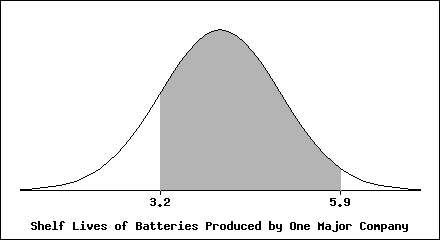
\includegraphics[width=\linewidth]{images/webwork-39-image-1.png}
\end{sbspanel}%
\end{sidebyside}%
\par\smallskip%
\noindent\textbf{\blocktitlefont Answer}.\hypertarget{g:answer:idp414}{}\quad{}\(0.818594614120363\)%
\end{inlineexercise}%
While we are at it, can we "go backwards" and figure out the mean and variance if given some probabilities.%
\begin{inlineexercise}{WebWork - Computing Regular Normal Probabilities.}{g:exercise:idp415}%
Consider a normal distribution curve where the middle 45 \% of the area under the curve lies above the interval ( 3 , 15 ). Use this information to find the mean,  \(\mu\) , and the standard deviation, \(\sigma\) , of the distribution.%
\par
a)  \(\mu =\) \fillin{9.090909090909092}%
\par
b)  \(\sigma =\) \fillin{9.090909090909092}%
\par\smallskip%
\noindent\textbf{\blocktitlefont Answer 1}.\hypertarget{g:answer:idp416}{}\quad{}\(9\)%
\par\smallskip%
\noindent\textbf{\blocktitlefont Answer 2}.\hypertarget{g:answer:idp417}{}\quad{}\(10.0375\)%
\end{inlineexercise}%
\begin{theorem}{Normal Distribution Maximum.}{}{x:theorem:NormalCurveMax}%
The maximum of the normal distribution probability function occurs when \(x = \mu\)%
\end{theorem}
\begin{proof}{}{g:proof:idp418}
Take the derivative of the probability function to get%
\begin{equation*}
\frac{\sqrt{2} {\left(\mu - x\right)} e^{\left(-\frac{{\left(\mu - x\right)}^{2}}{2 \, \sigma^{2}}\right)}}{2 \, \sqrt{\pi} \sigma^{3}}
\end{equation*}
which is zero only when \(x = \mu\).  Easily by evaluating to the left and right of this value shows that this critical value yields a maximum.%
\end{proof}
%
\par
\begin{theorem}{Normal Distribution Points of Inflection.}{}{x:theorem:NormalPOI}%
Points of Inflection for the normal distribution probability function occurs when \(x = \mu + \sigma\) and \(x = \mu - \sigma\).%
\end{theorem}
\begin{proof}{}{g:proof:idp419}
Take the second derivative of the probability function to get%
\begin{equation*}
\frac{\sqrt{2} {\left(\mu + \sigma - x\right)} {\left(\mu - \sigma - x\right)} e^{\left(-\frac{\mu^{2}}{2 \, \sigma^{2}} + \frac{\mu x}{\sigma^{2}} - \frac{x^{2}}{2 \, \sigma^{2}}\right)}}{2 \, \sqrt{\pi} \sigma^{5}}
\end{equation*}
which is zero only when \(x = \mu \pm \sigma\).  Easily by evaluating to the left and right of this value shows that these critical values yield points of inflection.%
\end{proof}
%
\par
Notice that the work needed to complete the integrals over the entire domain above was pretty serious. To determine probabilities for a given interval is however not possible in general and therefore approximations are needed. When using TI graphing calculators, you can use%
\begin{equation*}
P( a \lt x \lt b ) = \text{normalcdf}(a,b,\mu, \sigma).
\end{equation*}
Or you can use the calculator below.%
\par
\leavevmode%
\begin{sageinput}
@interact(layout=dict(top=[['a', 'b']],bottom=[['mu','sigma']]))
def _(a=input_box(-2,width=10,label='a = '),b=input_box(2,width=10,label='b = '),mu=input_box(0,width=8,label='$\mu = $'),sigma=input_box(1,width=8,label='$\sigma = $')):
    f = e^(-((x-mu)/sigma)^2/2)/(sigma*sqrt(2*pi))
    P = integral_numerical(f,a,b)[0]
    print "P("+str(a)+" < X < "+str(b)+") ~= "+str(P)
\end{sageinput}
%
\begin{inlineexercise}{WebWork - Applying Normal Probabilities.}{g:exercise:idp420}%
The physical fitness of an athlete is often measured by how much oxygen the athlete takes in (which is recorded in milliliters per kilogram, ml\slash{}kg).  The mean maximum oxygen uptake for elite athletes has been found to be \(70\) with a standard deviation of \(9.3\).  Assume that the distribution is approximately normal.%
\par
(a) \(\) What is the probability that an elite athlete has a maximum oxygen uptake of at least \(70\) ml\slash{}kg?%
\par
answer: \fillin{4.545454545454546}%
\par
(b) \(\) What is the probability that an elite athlete has a maximum oxygen uptake of \(65\) ml\slash{}kg or lower?%
\par
answer: \fillin{4.545454545454546}%
\par
(c) \(\) Consider someone with a maximum oxygen uptake of \(25\) ml\slash{}kg.  Is it likely that this person is an elite athlete? Write "YES" or "NO."%
\par
answer: \fillin{4.545454545454546}%
\par\smallskip%
\noindent\textbf{\blocktitlefont Answer 1}.\hypertarget{g:answer:idp421}{}\quad{}\(0.499999999013163\)%
\par\smallskip%
\noindent\textbf{\blocktitlefont Answer 2}.\hypertarget{g:answer:idp422}{}\quad{}\(0.295414734181962\)%
\par\smallskip%
\noindent\textbf{\blocktitlefont Answer 3}.\hypertarget{g:answer:idp423}{}\quad{}NO%
\end{inlineexercise}%
\end{sectionptx}
%
%
\typeout{************************************************}
\typeout{Section 9.3 Chi-Square Distribution}
\typeout{************************************************}
%
\begin{sectionptx}{Chi-Square Distribution}{}{Chi-Square Distribution}{}{}{x:section:ChiSquareDistribution}
The following distribution is related to both the Normal Distribution and to the Gamma Distribution. Initially, consider a gamma distribution with probability function%
\begin{equation*}
\frac{x^{r-1} \cdot e^{-x / \mu}}{\Gamma(r) \cdot \mu^r}.
\end{equation*}
Replacing \(\mu = 2\) and r with r\slash{}2 gives%
\begin{equation*}
\frac{x^{r/2-1} \cdot e^{-x/2}}{\Gamma(r/2) \cdot 2^{r/2}}
\end{equation*}
which is given a special name below.%
\par
\begin{definition}{Chi-Square Probability Function.}{x:definition:ChiSquarePF}%
Given an natural number r, suppose X is a random variable over the space \(R = (0,\infty)\) with probability function given by%
\begin{equation*}
f(x) = \frac{x^{r/2-1} e^{-x/2} }{\Gamma(r/2) 2^{r/2}}.
\end{equation*}
Then X has a Chi-Square distribution with r degrees of freedom. This is often denoted \(\chi^2(r)\).%
\end{definition}
%
\par
\leavevmode%
\begin{sageinput}
# Chi-Square Grapher
@interact
def _(r=slider(1,20,1,3,label='r =')):
    f = x^(r/2-1)*e^(-x/2)/(gamma(r/2)*2^(r/2))
    plot(f,x,0,20).show()
\end{sageinput}
%
\par
\begin{theorem}{\(\chi^2\) statistics.}{}{x:theorem:ChiSquareStatistics}%
%
\begin{equation*}
\mu = r
\end{equation*}
%
\begin{equation*}
\sigma^2 = 2r
\end{equation*}
%
\begin{equation*}
\gamma_1 = 2 \sqrt{2/r}
\end{equation*}
%
\begin{equation*}
\gamma_2 = \frac{12}{r} + 3
\end{equation*}
\end{theorem}
%
\par
\begin{theorem}{Relationship between Normal and \(\chi^2\).}{}{x:theorem:NormalVsChiSquare}%
If \(Z_1, Z_2, ..., Z_r\) are r standard normal variables, then%
\begin{equation*}
X = \sum_{k=1}^r Z_k^2
\end{equation*}
is \(\chi^2(r)\).\end{theorem}
%
\par
It also can be difficult to compute Chi-Square probabilities manually so you will perhaps want to use a numerical approximation in this case as well. The TI graphing calculator can be used with \(\chi ^2\)cdf(a,b,r).  Or, you can use the calculator below.%
\par
On your graphing calculator, you can use \(P(a \le X \le b) \approx \Chi^2\)cdf(a,b,r).%
\par
\leavevmode%
\begin{sageinput}
# Chi-Square Calculator
@interact(layout=dict(top=[['a', 'b']],bottom=[['r']]))
def _(a=input_box(0,width=10,label='a = '),b=input_box(2,width=10,label='b = '),r=input_box(2,width=8,label='r =')):
    f = x^(r/2-1)*e^(-x/2)/(gamma(r/2)*2^(r/2))
    P = numerical_integral(f,a,b)[0]
    print "P("+str(a)+" < X < "+str(b)+") ~= "+str(P)
\end{sageinput}
%
\end{sectionptx}
%
%
\typeout{************************************************}
\typeout{Section 9.4 Other "Bell Shaped" distributions}
\typeout{************************************************}
%
\begin{sectionptx}{Other "Bell Shaped" distributions}{}{Other "Bell Shaped" distributions}{}{}{x:section:OtherBellShapedDistributions}
The Normal distribution discussed above is very important when doing statistical analysis. It however is not the only distribution that is symmetrical about the mean and looks like a bell.  In this section, we consider two other options-{}-{}one which is virtually useless and another which is very useful.%
\par
\begin{definition}{The Cauchy Distribution.}{x:definition:CauchyPF}%
Consider a continuous random variable on the real numbers defined by%
\begin{equation*}
f(x) = \frac{1/\pi}{1+x^2}.
\end{equation*}
A random variable with this probability function is said to be a Cauchy Distribution.%
\end{definition}
%
\begin{theorem}{The Cauchy Distribution.}{}{x:theorem:CauchyStatistics}%
%
\begin{equation*}
f(x) = \frac{1/\pi}{1+x^2}
\end{equation*}
is a probability function on \((-\infty, \infty)\).\end{theorem}
\begin{proof}{}{g:proof:idp424}
Easily, note that%
\begin{equation*}
\int_{-\infty}^{\infty} \frac{1}{1+x^2} dx = arctan(\infty) - arctan(-\infty) = \pi/2 - (-\pi/2) = \pi.
\end{equation*}
Dividing by \(\pi\) gives the Cauchy probability function integrates to 1.\end{proof}
\begin{sageinput}
n &- 10
p &- 0.3

paste('Probability Function')
dcauchy(x, location = 0, scale = 1, log = FALSE)   # gives the probability function
paste('Distribution function')
pcauchy(q, location = 0, scale = 1, lower.tail = TRUE, log.p = FALSE)
   # gives the distribution function
paste('A random sample')
rcauchy(n, location = 0, scale = 1)    # gives a random sample of 15 items from b(n,p)

x=seq(-4,4,length=200)
y=dcauchy(x,dcauchy(x, location = 0, scale = 1, log = FALSE))
plot(x,y,type="l",lwd=2,col="red",ylab="p")
\end{sageinput}
Now that we have a probability function, it is important to determine its mean and variance. It should be obvious that when doing so using the Cauchy probability function, problems quickly arise.  Indeed,%
\begin{equation*}
\int_{-\infty}^{\infty} x \frac{1}{1+x^2} dx = (1/2) ( \ln( | \infty |) - \ln( | -\infty |)
\end{equation*}
which is problematic.  Further, for the variance%
\begin{equation*}
\int_{-\infty}^{\infty} x^2 \frac{1}{1+x^2} dx 
\end{equation*}
and note that the integrand does not converge to 0 at the endpoints and therefore the integral is automatically considered divergent.  Thus it is reasonable to note that the Cauchy distribution has no variance.%
\par
On the other hand, there is another "bell-shaped" distribution that is useful and its random variable can be created by using a mixture of a normal variable and a \(\Chi^2\) variable.%
\par
\begin{definition}{Student-t Distribution.}{x:definition:StudenttPF}%
Suppose Z is a standard normal variable and Y is \(\Chi^2(r)\) with Y and Z independent.  Define a new random variable%
\begin{equation*}
T = \frac{Z}{\sqrt(Y/r)}.
\end{equation*}
Then, T is said to have a (Student) t distribution with probability function given by%
\begin{equation*}
\frac{\Gamma \left ( \frac{n+1}{2} \right ) }{\sqrt{n \pi} \Gamma \left ( \frac{n}{2} \right ) } \left ( 1 + \frac{x^2}{n}\right )^{ - \left ( \frac{n+1}{2} \right )}  
\end{equation*}
%
\end{definition}
 The good news is that this distribution is useful and its properties are presented below without proof. \begin{theorem}{Student t-distribution properties.}{}{x:theorem:StudenttStatistics}%
For the Student t variable T defined above,%
\begin{equation*}
\mu = 0
\end{equation*}
and if r\textgreater{}2%
\begin{equation*}
\sigma^2 = \frac{r}{r-2}
\end{equation*}
and if r\textgreater{}3%
\begin{equation*}
\gamma_1 = 0
\end{equation*}
and if r\textgreater{}4%
\begin{equation*}
\gamma_2 = \frac{6}{r-4} + 3.
\end{equation*}
%
\end{theorem}
%
\par
\begin{example}{Similarity between Normal and t-distributions for larger n.}{g:example:idp425}%
Consider the probabilities \(P(-2 \le Z \le 2)\) vs \(P(-2 \le T \le 2)\) for a t-distribution with r=30 degrees of freedom.%
\par
For normal,%
\begin{equation*}
P(-2 \le Z \le 2) = \Phi(2) - \Phi(-2) = 0.9545
\end{equation*}
while for t,%
\begin{equation*}
P(-2 \le T \le 2) = 0.9454.
\end{equation*}
%
\end{example}
%
\par
\leavevmode%
\begin{sageinput}
# Display the Student's t distributions with various
# degrees of freedom and compare to the normal distribution
# Copied from www.statmethods.net

x <- seq(-4, 4, length=100)
hx <- dnorm(x)

degf <- c(1, 3, 8, 30)
colors <- c("red", "blue", "darkgreen", "gold", "black")
labels <- c("df=1", "df=3", "df=8", "df=30", "normal")

plot(x, hx, type="l", lty=2, xlab="x value",
  ylab="Density", main="Comparison of t Distributions")

for (i in 1:4){
  lines(x, dt(x,degf[i]), lwd=2, col=colors[i])
}

legend("topright", inset=.05, title="Distributions",
  labels, lwd=2, lty=c(1, 1, 1, 1, 2), col=colors)
\end{sageinput}
%
\end{sectionptx}
%
%
\typeout{************************************************}
\typeout{Section 9.5 Generating Functions for Normal and Associated Distributions}
\typeout{************************************************}
%
\begin{sectionptx}{Generating Functions for Normal and Associated Distributions}{}{Generating Functions for Normal and Associated Distributions}{}{}{x:section:NormalAssociatedGeneratingFunctions}
\hyperref[x:definition:DefnMomentGeneratingFunction]{Moment Generating Functions~{\xreffont\ref{x:definition:DefnMomentGeneratingFunction}}} can be derived for each of the distributions in this chapter.%
\par
\begin{theorem}{Moment Generating Function for Normal.}{}{x:theorem:NormalMGF}%
Presuming \(t \gt 0\) and%
\begin{equation*}
M(t) = e^{t \mu+\frac{1}{2}t^2\sigma^2}
\end{equation*}
%
\end{theorem}
\begin{proof}{}{g:proof:idp426}
Using the \hyperref[x:definition:NormalPF]{Normal probability function~{\xreffont\ref{x:definition:NormalPF}}},%
\begin{align*}
M(t) & = \int_{-\infty}^{\infty} e^{tx} \frac{1}{\sigma \sqrt{2 \pi}} e^{ -\left ( \frac{x-\mu}{\sigma} \right ) ^2 / 2}\\
& = \int_{-\infty}^{\infty} e^{tx} \frac{1}{\sigma \sqrt{2 \pi}} e^{ -\left ( \frac{x-\mu}{\sigma} \right ) ^2 / 2} dx\\
& = \int_{-\infty}^{\infty} e^{t(z \sigma + \mu)} \frac{1}{\sqrt{2 \pi}} e^{  -z ^2 / 2} dz\\
& = e^{t \mu} \int_{-\infty}^{\infty}  \frac{1}{\sqrt{2 \pi}} e^{  -(z ^2 - 2t z \sigma ) / 2} dz\\
& = = e^{t \mu} \int_{-\infty}^{\infty}  \frac{1}{\sqrt{2 \pi}} e^{  -(z ^2 - 2t z \sigma + t^2 \sigma^2 - t^2 \sigma^2 ) / 2} dz\\
& = e^{t \mu+\frac{1}{2}t^2\sigma^2} \int_{-\infty}^{\infty}  \frac{1}{\sqrt{2 \pi}} e^{  -\left (z - t \sigma \right )^2 / 2} dz\\
& = e^{t \mu+\frac{1}{2}t^2\sigma^2} \cdot 1 
\end{align*}
where the final integral is just a shifted standard normal and therefore has value 1.%
\end{proof}
 \begin{corollary}{Normal Properties via Moment Generating Function.}{}{g:corollary:idp427}%
For the Normal variable X,%
\begin{equation*}
M(0) = 1
\end{equation*}
%
\begin{equation*}
M'(0) = \mu
\end{equation*}
%
\begin{equation*}
M''(0) = \sigma^2 + \mu^2
\end{equation*}
%
\end{corollary}
\begin{proof}{}{g:proof:idp428}
%
\begin{equation*}
M(0) = e^{0 \mu+\frac{1}{2}0^2\sigma^2} = e^0 = 1.
\end{equation*}
Continuing,%
\begin{equation*}
M'(t) = {\left(\sigma^2 t + \mu \right)} e^{\left(\frac{1}{2} \sigma^2 t^{2} + \mu t \right)}
\end{equation*}
and therefore%
\begin{equation*}
M'(0) = {\left(\sigma^2 0 + \mu \right)} e^{\left(\frac{1}{2} \sigma^2 0^{2} + \mu 0 \right)} = \mu e^0 = \mu.
\end{equation*}
Continuing with the second derivative,%
\begin{equation*}
M''(t) = {\left(\sigma^2 t + \mu\right)}^2 e^{\left(\frac{1}{2} \sigma^2 t^2 + \mu t\right)} + \sigma^2 e^{\left(\frac{1}{2} \sigma^2 t^2 + \mu t\right)}
\end{equation*}
and therefore%
\begin{equation*}
M''(0) = {\left(\sigma^2 0 + \mu\right)}^2 e^{\left(\frac{1}{2} \sigma^2 0^2 + \mu 0\right)} + \sigma^2 e^{\left(\frac{1}{2} \sigma^2 0^2 + \mu 0\right)} = \mu^2 + \sigma^2 
\end{equation*}
which is the squared mean plus the variance for the normal distribution.%
\end{proof}
%
\par
\begin{theorem}{Moment Generating Function for Chi-Square.}{}{x:theorem:ChiSquareMGF}%
Presuming \(t \gt 0\) and%
\begin{equation*}
M(t) = \left ( \frac{1}{1-2t} \right )^{r/2}
\end{equation*}
%
\end{theorem}
\begin{proof}{}{g:proof:idp429}
Using the \hyperref[x:definition:ChiSquarePF]{Chi-Square probability function~{\xreffont\ref{x:definition:ChiSquarePF}}},%
\begin{align*}
M(t) & = \int_0^{\infty} e^{tx} \frac{x^{r/2-1} e^{-x/2} }{\Gamma(r/2) 2^{r/2} } dx\\
& = \int_0^{\infty} \frac{x^{r/2-1} e^{-x(1-2 t)/2} }{\Gamma(r/2) 2^{r/2}} dx\\
& = \int_0^{\infty} \frac{\left ( \frac{u}{1-2t} \right )^{r/2-1} e^{-u/2} }{\Gamma(r/2) 2^{r/2} } \frac{1}{1-2t} du\\
& = \left ( \frac{1}{1-2t} \right )^{r/2} \int_0^{\infty} \frac{u^{r/2-1} e^{-u/2} }{\Gamma(r/2) 2^{r/2}} du\\
& = \left ( \frac{1}{1-2t} \right )^{r/2}
\end{align*}
where the final integral is again Chi-Square and therefore has value 1.%
\end{proof}
 \begin{corollary}{Chi-Square Properties via Moment Generating Function.}{}{g:corollary:idp430}%
For the Chi-Square variable X,%
\begin{equation*}
M(0) = 1
\end{equation*}
%
\begin{equation*}
M'(0) = r = \mu
\end{equation*}
%
\begin{equation*}
M''(0) = 2r + r^2 = \sigma^2 + \mu^2
\end{equation*}
%
\end{corollary}
\begin{proof}{}{g:proof:idp431}
%
\begin{equation*}
M(0) = \left ( \frac{1}{1-2 \cdot 0} \right )^{r/2} = 1.
\end{equation*}
Continuing,%
\begin{equation*}
M'(t) = \frac{r {\left(-2 t + 1\right)}^{\frac{1}{2} r - 1}}{{\left(-2 t + 1 \right)}^{r}}
\end{equation*}
and therefore%
\begin{equation*}
M'(0) = \frac{r {\left(-2 \cdot 0 + 1\right)}^{\frac{1}{2} r - 1}}{{\left(-2 \cdot 0 + 1 \right)}^{r}} = \frac{r}{1} = r.
\end{equation*}
Continuing with the second derivative,%
\begin{equation*}
M''(t) = -\frac{{\left(r - 2\right)} r {\left(-2 t + 1\right)}^{\frac{1}{2} r - 2}}{{\left(-2 t + 1\right)}^{r}} + \frac{2 r^{2} {\left(-2 t + 1\right)}^{r - 2}}{{\left(-2 t + 1\right)}^{\frac{3}{2} r}}
\end{equation*}
and therefore%
\begin{align*}
M''(0) & = -\frac{{\left(r - 2\right)} r {\left(-2 \cdot 0 + 1\right)}^{\frac{1}{2} r - 2}}{{\left(-2 \cdot 0 + 1\right)}^{r}} + \frac{2 r^{2} {\left(-2 \cdot 0 + 1\right)}^{r - 2}}{{\left(-2 \cdot 0 + 1\right)}^{\frac{3}{2} r}} \\
& = -\frac{{\left(r - 2\right)} r }{1} + \frac{2 r^{2} }{1}= 2r + r^2 = \sigma^2 + \mu^2
\end{align*}
which is the squared mean plus the variance for the normal distribution.%
\end{proof}
%
\par
It is interesting to note that the moment generating functions are not defined for the \hyperref[x:definition:CauchyPF]{Cauchy Distribution~{\xreffont\ref{x:definition:CauchyPF}}} or for the \hyperref[x:definition:StudenttPF]{Student's t distribution~{\xreffont\ref{x:definition:StudenttPF}}}.%
\end{sectionptx}
%
%
\typeout{************************************************}
\typeout{Section 9.6 Normal Distribution as a Limiting Distribution}
\typeout{************************************************}
%
\begin{sectionptx}{Normal Distribution as a Limiting Distribution}{}{Normal Distribution as a Limiting Distribution}{}{}{x:section:NormalAsLimitingDistribution}
Over the past several chapters you should have noticed that many distributions have skewness and kurtosis formulae which have limiting values of 0 and 3 respectively. This means that each of those distributions which can be approximated by the normal distribution for "large" parameter values.%
\par
To see how this works, consider a "random" distribution in the following two interactive experiments.  For the first graph below, a sequence of N random samples, each of size r, ranging from 0 to "Range" is generated and graphed as small data points.  As the number of samples N and the sample size r increase, notice that the data seems to cover the entire range of possible values relatively uniformly.  (For this scatter plot note that each row represents the data for one sample of size r.  The larger the N, the greater the number of rows.)  Each row is averaged and that mean value is plotted on the graph as a red circle.  If you check the "Show\textunderscore{}Mean" box, the mean of these circles is indicated by the green line in the middle of the plot.%
\par
For the second graph below, the means are collected and the relative frequency of each is plotted.  As N increases, you should see that the results begin to show an interesting tendency.   As you increase the data range, you may notice this graph has a larger number of data values.  Smoothing groups this data into intervals of length two for perhaps a graph with less variability.%
\par
Consider each of the following:%
\begin{itemize}[label=\textbullet]
\item{}As N increases with single digit values of r, what appears to happen to the mean and range of the means?  How does increasing the data range from 1-100 to 1-200 or 1-300 affect these results?%
\item{}As N increases (say, for a middle value of r), what appears to happen to the means?  How does increasing the data range from 1-100 to 1-200 or 1-300 affect these results?%
\item{}As r increases (say, for a middle value of N), what appears to happen to the range of the averages?  Does your conclusion actually depend upon the value of N?  (Look at the graph and don't worry about the actual numerical values.) How does increasing N for the second graph affect the skewness and kurtosis of that graph?  Do things change significantly as r is increased?%
\end{itemize}
%
\par
\leavevmode%
\begin{sageinput}
var('n,k')
from sage.finance.time_series import TimeSeries

@interact(layout=dict(top=[['Range'],['Show_Mean', 'Smoothing']],  
bottom=[['N'],['r']]))

def _(Range=[100,200,300,500],N=slider(5,200,2,2,label="N = Number of Samples"),r=slider(3,200,1,2,label="r = Sample Size"),Show_Mean=False,Smoothing=False):
    R=[1..N]     #  R ranges over the number of samples...will point to the list of averages
    rangemax = Range

    data = random_matrix(ZZ,N,r,x=rangemax)
    datapoints = []
    avg_values = []
    avg_string = []
    averages = []
    for n in range(N):
        temp = 0
        for k in range(r):
            datapoints += [(data[n][k],n)]
            temp += data[n][k]
        avg_values.append(round(temp/r))
        if Smoothing:
            avg_string.append(str(2*round((temp/r)/2)))    
        else:
            avg_string.append(str(round(temp/r)))
            
        averages += [(round(temp/r),n)]   #  make these averages integers for use in grouping later
    SCAT = scatter_plot(datapoints,markersize=2,edgecolor='red',figsize=(10,4),axes_labels=['Sample Values','Sample Number'])
    AVGS = scatter_plot(averages,markersize=50,edgecolor='blue',marker='o',figsize=(7,4))
    
    freqslist = frequency_distribution(avg_string,1).function().items()
       
       
# compute sample statistics for the raw data as well as for the N averages
    Mean_data = (sum(sum(data))/(N*r)).n()
#    STD_data = sqrt(sum(sum( (data-Mean_data)^2 ))/(N*r)).n()
    Mean_averages = mean(avg_values).n()
#    STD_averages = sqrt(variance(avg_values).n())
#    print "Data mean =",Mean_data," vs Mean of the averages =",Mean_averages
#    print "Data STD = ",STD_data," vs Standard Dev of avgs =", STD_averages
    if Show_Mean:
        avg_line = line([(Mean_data,0),(Mean_data,N-1)],rgbcolor='green',thickness=10)
        avg_text = text('xbar',(Mean_data,N),horizontal_alignment='right',rgbcolor='green')
    else:
        avg_line = Graphics()
        avg_text = Graphics()
            
#  Plot a scatter plot exhibiting uniformly random data and the collection of averages 
    print(html("The random data plot on the left with each row representing a sample with size determined by\n"+
         "the slider above and each circle representing the average for that particular sample.\n"+
         "First, keep sample size relatively low and increase the number of samples.  Then, \n"+
         "watch what happens when you slowly increase the sample size."))

    
#  Plot the relative frequencies of the grouped sample averages
    print(html("Now, the averages (ie. the circles) from above are collected and counted\n"+
         "with the relative frequency of each average graphed below.  For a relatively large number of\n"+
         "samples, notice what seems to happen to these averages as the sample size increases."))
    if Smoothing:
        binRange = Range//2
    else:
        binRange = Range
    
    # normed=True  # if you want to have relative frequencies below
    
    his_low = 2*rangemax/7
    his_high = 5*rangemax/7
    
    T = histogram(avg_values,normed=False,bins=binRange,range=(his_low,his_high),axes_labels=['Sample Averages','Frequency']) 
    #T = TimeSeries(avg_values).plot_histogram(axes_labels=['Sample Averages','Frequency'])   
    
    pretty_print('Scatter Plot of random data.  Horizontal is number of samples.')
    (SCAT+AVGS+avg_line+avg_text).show()
    pretty_print('Histogram of Sample Averages')
    T.show(figsize=(5,2))
\end{sageinput}
%
\par
\leavevmode%
\begin{sageinput}
var('n,k')
from sage.finance.time_series import TimeSeries

@interact(layout=dict(top=[['Range'],['Show_Mean', 'Smoothing']],  
bottom=[['N'],['r']]))

def _(Range=[100,200,300,500],N=slider(5,200,2,2,label="N = Number of Samples"),r=slider(3,200,1,2,label="r = Sample Size"),Show_Mean=False,Smoothing=False):
    R=[1..N]     #  R ranges over the number of samples...will point to the list of averages
    rangemax = Range

    data = random_matrix(ZZ,N,r,x=rangemax)
    datapoints = []
    avg_values = []
    avg_string = []
    averages = []
    for n in range(N):
        temp = 0
        for k in range(r):
            datapoints += [(data[n][k],n)]
            temp += data[n][k]
        avg_values.append(round(temp/r))
        if Smoothing:
            avg_string.append(str(2*round((temp/r)/2)))    
        else:
            avg_string.append(str(round(temp/r)))
            
        averages += [(round(temp/r),n)]   #  make these averages integers for use in grouping later
    SCAT = scatter_plot(datapoints,markersize=2,edgecolor='red',figsize=(10,4),axes_labels=['Sample Values','Sample Number'])
    AVGS = scatter_plot(averages,markersize=50,edgecolor='blue',marker='o',figsize=(7,4))
    
    freqslist = frequency_distribution(avg_string,1).function().items()
       
       
# compute sample statistics for the raw data as well as for the N averages
    Mean_data = (sum(sum(data))/(N*r)).n()
#    STD_data = sqrt(sum(sum( (data-Mean_data)^2 ))/(N*r)).n()
    Mean_averages = mean(avg_values).n()
#    STD_averages = sqrt(variance(avg_values).n())
#    print "Data mean =",Mean_data," vs Mean of the averages =",Mean_averages
#    print "Data STD = ",STD_data," vs Standard Dev of avgs =", STD_averages
    if Show_Mean:
        avg_line = line([(Mean_data,0),(Mean_data,N-1)],rgbcolor='green',thickness=10)
        avg_text = text('xbar',(Mean_data,N),horizontal_alignment='right',rgbcolor='green')
    else:
        avg_line = Graphics()
        avg_text = Graphics()
            
#  Plot a scatter plot exhibiting uniformly random data and the collection of averages 
    print(html("The random data plot on the left with each row representing a sample with size determined by\n"+
         "the slider above and each circle representing the average for that particular sample.\n"+
         "First, keep sample size relatively low and increase the number of samples.  Then, \n"+
         "watch what happens when you slowly increase the sample size."))

    
#  Plot the relative frequencies of the grouped sample averages
    print(html("Now, the averages (ie. the circles) from above are collected and counted\n"+
         "with the relative frequency of each average graphed below.  For a relatively large number of\n"+
         "samples, notice what seems to happen to these averages as the sample size increases."))
    if Smoothing:
        binRange = Range//2
    else:
        binRange = Range
    
    # normed=True  # if you want to have relative frequencies below
    
    his_low = 2*rangemax/7
    his_high = 5*rangemax/7
    
    T = histogram(avg_values,normed=False,bins=binRange,range=(his_low,his_high),axes_labels=['Sample Averages','Frequency']) 
    #T = TimeSeries(avg_values).plot_histogram(axes_labels=['Sample Averages','Frequency'])   
    
    pretty_print('Scatter Plot of random data.  Horizontal is number of samples.')
    (SCAT+AVGS+avg_line+avg_text).show()
    pretty_print('Histogram of Sample Averages')
    T.show(figsize=(5,2))
\end{sageinput}
%
\par
So, even with random data, if you are to consider the arrangement of the collected means rather than the arrangement of the actual data then the means appear to have a bell-shaped distribution as well.%
\end{sectionptx}
%
%
\typeout{************************************************}
\typeout{Section 9.7 Central Limit Theorem}
\typeout{************************************************}
%
\begin{sectionptx}{Central Limit Theorem}{}{Central Limit Theorem}{}{}{x:section:CentralLimitTheoremSection}
Often, when one wants to solve various scientific problems, several assumptions will be made regarding the nature of the underlying setting and base their conclusions on those assumptions.  Indeed, if one is going to use a Binomial Distribution or a Negative Binomial Distribution, an assumption on the value of p is necessary.  For Poisson and Exponential Distributions, one must know the mean.  For Normal Distributions, one must assume values for both the mean and the standard deviation.   Where do these values come from?  Often, one may perform a preliminary study and obtain a sample statistic...such as a sample mean or a relative frequency and use these values for μ or p.%
\par
But what is the underlying distribution of these sample statistics?  The Central Limit Theorem gives the answer...%
\par
The results from the previous section illustrate the tendency for bell-shaped distributions. This tendency can be described more mathematically through the following theorem. It is presented here without proof.%
\par
\begin{theorem}{Central Limit Theorem.}{}{x:theorem:CentralLimitTheorem}%
Presume X is a random variable from a distribution with known mean \(\mu\) and known variance \(\sigma_x^2\). For some natural number n, sample the distribution repeatedly creating a string of random variables denoted \(X_1, X_2, ... , X_n\) and set \(\overline{X} = \frac{\sum X_k}{n}\).%
\par
Then, \(\overline{X}\) is approximately normally distributed with mean \(\mu\) and variance \(\sigma^2 = \frac{\sigma_x^2}{n}\).%
\end{theorem}
%
\par
Often the Central Limit Theorem is stated more formally using a conversion to standard units. Indeed, the theorem indicates that the random variable \(\overline{X}\) has variance \(\frac{\sigma^2}{n}\) which means as n grows this variance approaches 0. So, the limiting random variable has a zero variance and therefore is no longer a random variable. To avoid this issue, the Central Limit Theorem is often stated as:%
\par
For random variables%
\begin{equation*}
W_n = \frac{\overline{X} - \mu}{\sigma/ \sqrt{n}}
\end{equation*}
with corresponding distribution function \(F_n(W_n)\),%
\begin{equation*}
\lim_{n \rightarrow \infty} F_n(c) = \int_{-\infty}^c \frac{1}{\sqrt{2 \pi}} e^{-z^2/2} dz = \Phi(c)
\end{equation*}
that is, the standard normal distribution function.%
\par
While we are at it, we can again "go backwards" and figure out the mean and variance if given some probabilities.%
\begin{inlineexercise}{WebWork - Computing probabilities on \(\overline{X}\).}{g:exercise:idp432}%
A sample of \(n= 20\) observations is drawn from a normal population with \(\mu = 1000\) and \(\sigma = 180\).  Find each of the following:%
\par
A. \(P(\bar{X} > 1076)\)%
\par
Probability = \fillin{6.818181818181818}%
\par
B. \(P(\bar{X} \lt  931)\)%
\par
Probability = \fillin{6.818181818181818}%
\par
C. \(P(\bar{X} > 955)\)%
\par
Probability = \fillin{6.818181818181818}%
\par\smallskip%
\noindent\textbf{\blocktitlefont Answer 1}.\hypertarget{g:answer:idp433}{}\quad{}\(0.0294971914033473\)%
\par\smallskip%
\noindent\textbf{\blocktitlefont Answer 2}.\hypertarget{g:answer:idp434}{}\quad{}\(0.0432350967176791\)%
\par\smallskip%
\noindent\textbf{\blocktitlefont Answer 3}.\hypertarget{g:answer:idp435}{}\quad{}\(0.868223760375634\)%
\end{inlineexercise}%
\begin{example}{Exponential X vs Normal \(\overline{X}\).}{g:example:idp436}%
Consider an exponential variable X with mean time till first success of \(\mu = 4\).  Then, \(\sigma = 2\) using the exponential formulas.%
\par
You can use the exponential probability function to compute probabilities dealing with X. Indeed,%
\begin{equation*}
P(X \lt 3.9) = F(3.9) = 1 - e^{-3.9/4} \approx 0.6228 .
\end{equation*}
%
\par
If instead you plan to sample from this distribution n=32 times, the Central Limit Theorem implies that you will get a random variable \(\overline{X}\) which has an approximate normal distribution with the same mean but with new variance \(\sigma_{\overline{X}}^2 = \frac{4}{32} = \frac{1}{8}\).  Therefore%
\begin{equation*}
P( \overline{X} \lt 3.9 ) \approx normalcdf(0,3.9,4,sqrt(1/8)) = 0.3886 .
\end{equation*}
%
\end{example}
%
\par
When converting probability problems from continuous (such as exponential or uniform) then no adjustment to the question is needed since you are approximating one area with another area. However, when converting probability problems from discrete (such as binomial or geometric) then you need to consider how the interval would need to be adjusted so that histogram areas for the discrete problem would relate to areas under the normal curve. Generally, you will need to expand the stated interval each way by 1\slash{}2.%
\par
The Central Limit Theorem provides that regardless of the distribution of X, the distribution of an average of X's is approximately normally distributed. However, it also shows why X may also be approximated for some distributions using the normal distribution as certain parameters are allowed to increase. Below, you can see how Binomial and Poisson distributions can be approximated directly using the Normal distribution.%
\par
Toward that end, for \(0 \lt p \lt 1\) consider a sequence of Bernoulli trials \(Y_1, Y_2, ..., Y_n\) with each over the space \textbraceleft{}0,1\textbraceright{}. Then,%
\begin{equation*}
X = \sum_{k=1}^n Y_k
\end{equation*}
is a Binomial variable.%
\begin{theorem}{The Binomial Distribution approximately Normal if n large..}{}{x:theorem:BinomialApproximatelyNormal}%
Given a Binomial variable X with \(\mu = np\) and \(\sigma^2 = np(1-p)\), then X is approximately also normal with the same mean and variance so long as \(np \gt 5\) and \(n(1-p) \gt 5\).%
\end{theorem}
\begin{proof}{}{g:proof:idp437}
Using the Bernoulli variables \(Y_k\) each with mean p and variance p(1-p), note that the Central Limit Theorem applied to \(\overline{X} = \frac{\sum Y_k}{n}\) gives that%
\begin{equation*}
\frac{\overline{X}-p}{\sqrt{p(1-p)/n}}
\end{equation*}
is approximately standard normal. By multiplying top and bottom by n yields%
\begin{equation*}
\frac{\sum Y_k - np}{\sqrt{np(1-p)}}
\end{equation*}
is approximately standard normal. But \(\sum Y_k\) actually is the sum of the number of successes in n trials and is therefore a Binomial variable.%
\end{proof}
\begin{example}{Binomial as Normal.}{g:example:idp438}%
Binomial becomes normal as \(n \rightarrow \infty\).  Consider n = 50 and p = 0.3.  Then, \(\mu = 15\) and \(\sigma^2 = 10.5\).%
\par
Using the binomial formulas, for example,%
\begin{equation*}
P( X = 16 ) = \binom{50}{16} 0.3^{16} \cdot 0.7^{34} \approx 0.11470
\end{equation*}
Using the normal distribution,%
\begin{align*}
P( X = 16 ) & = P( 15.5 \lt X \lt 16.5) \\
& \approx normalcdf(15.5,16.5,15,sqrt(10.5)) \\
& = 0.11697
\end{align*}
Notice that these are very close.%
\end{example}
\begin{corollary}{The Poisson Distribution is approximately normal with \(\mu\) large..}{}{x:corollary:PoissonApproximatelyNormal}%
Given a Poisson variable X with \(\mu\) and \(\sigma^2 = \mu\) given, then X is approximately also normal with the same mean and variance so long as \(\mu \gt 5\).%
\end{corollary}
\begin{proof}{}{g:proof:idp439}
Note from before that the Poisson distribution function was derived by approximating with Binomial and letting n approach infinity. Therefore, by the previous theorem, the Poisson variable is also approximately Normal using the Poisson mean and variance rather than the binomial's. Indeed, in standard units%
\begin{equation*}
\frac{Y - \mu}{\sqrt{\mu}}
\end{equation*}
is approximately normal for large \(\mu\).%
\end{proof}
\begin{example}{Poisson as Normal.}{g:example:idp440}%
Poisson becomes normal as \(\mu \rightarrow \infty\).  Consider \(\mu = 20\).  Then, \(\sigma^2 = \mu = 20\).%
\par
Using the Poisson formulas, for example,%
\begin{equation*}
P( X = 19 ) = \frac{20^{19} e^{-20}}{19!} \approx 0.08883
\end{equation*}
Using the normal distribution,%
\begin{align*}
P( X = 19 ) & = P( 18.5 \lt X \lt 19.5) \\
& \approx normalcdf(18.5,19.5,20,sqrt(20)) \\
& = 0.08683
\end{align*}
Again, these are very close.%
\end{example}
\begin{theorem}{The Gamma is approximate Normal for \(\mu\) large..}{}{x:theorem:GammaApproximatelyNormal}%
Given a Gamma variable X with mean \(r \mu\) and variance \(r BLOB\) given, then X is approximately also normal with the same mean and variance so long as CONDITION????.%
\end{theorem}
\begin{example}{Gamma as Normal.}{g:example:idp441}%
Gamma becomes normal as \(r \rightarrow \infty\).  Assume that the average time till a first success is 12 minutes and that \(r = 8\).  Then, the mean for the Gamma distribution is \(\mu = 12 \cdot 8 = 96\) and \(\sigma^2 = 8 \cdot 12^2 = 1152\) and so \(\sigma \approx 33.9411\).%
\par
Using the Gamma formulas,%
\begin{align*}
P( 90 \le X \le 100 ) & = \int_{90}^{100} f(x) dx \\
& = 0.59252 - 0.47536 = 0.11716.
\end{align*}
Using the normal distribution,%
\begin{equation*}
P( 90 \le X \le 100) \approx normalcdf(90,100,96,33.9411) = 0.11707.
\end{equation*}
Amazingly, these are also very close.%
\end{example}
\begin{example}{Uniform X vs Normal \(\overline{X}\).}{g:example:idp442}%
Consider a discrete uniform variable X over R = \textbraceleft{}1,2,...,20\textbraceright{}.  Then, \(\mu = 10.5\) and \(\sigma = \frac{20^2-1^2}{20}\) using the uniform formulas.%
\par
You can use the uniform probability function to compute probabilities dealing with X. Indeed,%
\begin{equation*}
P(8 \le X \lt 12) = P(X \in \{8,9,10,11 \} = \frac{4}{20} = 1/5.
\end{equation*}
%
\par
If instead you plan to sample from this distribution n=49 times, the Central Limit Theorem implies that you will get a random variable \(\overline{X}\) which has an approximate normal distribution with the same mean but with new variance \(\sigma_{\overline{X}}^2 = \frac{199/20}{49} = \frac{199}{580}\).  Therefore, expanding the interval to include the boundaries of the corresponding histogram areas,%
\begin{equation*}
P( 8 \le \overline{X} \lt 12 ) = P(7.5 \le \overline{X} \le 11.5) \approx normalcdf(7.5,11.5,10.5,0.585750) \approx 0.9561 .
\end{equation*}
%
\end{example}
As these examples illustrate, you will have increasing success in approximating the desired probabilities so long as the distribution's corresponding parameter is allowed to be "sufficiently large". The mathematical reasoning this is true is not provided but depends upon the "Central Limit Theorem" discussed in the next section.%
\par
The above theorems allow you to utilize the normal distribution to compute approximate probabilities for the variable X in the stated distributions. This is not always true for all distributions since some do not have parameters which allow for approaching normality. However, regardless of the distribution the Central Limit Theorem always allows you to approximate probabilities if they involve an average of repeated attempts...that is, for variable \(\overline{X}\). This usefulness is illustrated in the examples below.%
\end{sectionptx}
%
%
\typeout{************************************************}
\typeout{Section 9.8 Summary}
\typeout{************************************************}
%
\begin{sectionptx}{Summary}{}{Summary}{}{}{x:section:NormalRelatedDistributionsSummary}
Here is a summary of the major points in this chapter:%
\par
TBA%
\end{sectionptx}
%
%
\typeout{************************************************}
\typeout{Section 9.9 Exercises}
\typeout{************************************************}
%
\begin{sectionptx}{Exercises}{}{Exercises}{}{}{x:section:NormalRelatedDistributionsExercises}
\begin{inlineexercise}{- Computing basic standard normal probabilities.}{g:exercise:idp443}%
Compute%
\begin{itemize}[label=\textbullet]
\item{}%
\begin{equation*}
P( Z \gt 0)
\end{equation*}
%
\item{}%
\begin{equation*}
P( Z \lt 0.892)
\end{equation*}
%
\item{}%
\begin{equation*}
P( Z \lt -0.892)
\end{equation*}
%
\item{}%
\begin{equation*}
P( -1.45 \lt Z \lt 2.37)
\end{equation*}
%
\item{}%
\begin{equation*}
P( -1 \lt Z \lt 1)
\end{equation*}
which is the probability of lying within 1 standard deviation of the mean.%
\item{}%
\begin{equation*}
P( -2 \lt Z \lt 2)
\end{equation*}
which is the probability of lying within 2 standard deviations of the mean.%
\item{}%
\begin{equation*}
P( -3 \lt Z \lt 3)
\end{equation*}
which is the probability of lying within 3 standard deviations of the mean.%
\item{}A value for a so that%
\begin{equation*}
P( Z \lt a) = 0.8
\end{equation*}
which would be the location of the 80th percentile.%
\end{itemize}
%
\end{inlineexercise}%
\begin{inlineexercise}{- Computing basic normal probabilities.}{g:exercise:idp444}%
Given \(\mu = 25\) and \(\sigma = 4\) compute%
\begin{equation*}
P(X \lt \mu)
\end{equation*}
%
\begin{equation*}
P( X \gt 26)
\end{equation*}
%
\begin{equation*}
P( X \gt 22)
\end{equation*}
%
\begin{equation*}
P( 20 \le X \le 26)
\end{equation*}
%
\end{inlineexercise}%
\begin{inlineexercise}{- IQ values.}{g:exercise:idp445}%
The Intelligence Quotient (IQ) is a measure of your ability to think and reason. Presuming that IQ scores are normally distributed with mean 100 and standard deviation 15, determine the location of the 90th percentile.  That is, the IQ score below which you will find approximately 90\% of other IQ scores.%
\end{inlineexercise}%
\end{sectionptx}
\end{chapterptx}
%
%
\typeout{************************************************}
\typeout{Chapter 10 Estimation}
\typeout{************************************************}
%
\begin{chapterptx}{Estimation}{}{Estimation}{}{}{x:chapter:IntervalEstimation}
%
%
\typeout{************************************************}
\typeout{Section 10.1 How Close is Close?}
\typeout{************************************************}
%
\begin{sectionptx}{How Close is Close?}{}{How Close is Close?}{}{}{x:section:IntervalEstimationIntroduction}
You should have noticed by now that repeatedly sampling from a given distribution will yield a variety of sample statistics such as \(\overline{x}\) as an estimate perhaps for the population mean \(\mu\) or \(\frac{Y}{n}\) as an estimate for the population likelihood of success p. In this section, you will see how these sample "point estimators" are actually the best possible choices.%
\par
In creating these point estimates repeatedly, you have noticed that the results will change somewhat over time. Indeed, flip a coin 20 times and you might expect 10 heads. However, in practice it is likely to 9 or 12 out of 20 and possible to get any of the other possible outcomes. This natural variation makes the point estimates noted above to almost certainly be in error. However one would expect that they should be close and the Central Limit Theorem does indicate that the distribution of sample means should be approximately normally distributed. Thus, instead of relying just on the value of the point estimate, you might want to investigate a way to determine a reasonable interval centered on the sample statistic in which you have some confidence the actual population statistic should belong. This leads to a discussion of interval estimates known as confidence intervals (using calculational tools) and statistical tolerance intervals (using order statistics).%
\par
In this chapter we first discuss how to determine appropriate methods for estimating the needed population statistics (point estimates) and then quantify how good they are (confidence intervals).%
\end{sectionptx}
%
%
\typeout{************************************************}
\typeout{Section 10.2 Interval Estimates - Chebyshev}
\typeout{************************************************}
%
\begin{sectionptx}{Interval Estimates - Chebyshev}{}{Interval Estimates - Chebyshev}{}{}{x:section:IntervalEstimationChebyshev}
An interval centered on the mean in which at least a certain proportion of the actual data must lie.%
\begin{theorem}{Chebyshev's Theorem.}{}{g:theorem:idp446}%
Given a random variable X with given mean \(\mu\) and standard deviation \(\sigma\), for \(a \in \mathbb{R}^+\) ,%
\begin{equation*}
P( \big | X - \mu \big | \lt a ) \gt 1 - \frac{\sigma^2}{a^2}
\end{equation*}
%
\end{theorem}
\begin{proof}{}{g:proof:idp447}
Notice that the variance of a continuous variable X is given by%
\begin{align*}
\sigma^2 & = \int_{-\infty}^{\infty} (x - \mu)^2 f(x) dx\\
& \ge \int_{-\infty}^{\mu-a} (x - \mu)^2 f(x) dx + \int_{\mu + a}^{\infty} (x - \mu)^2 f(x) dx\\
& \ge \int_{-\infty}^{\mu-a} a^2 f(x) dx + \int_{\mu + a}^{\infty} a^2 f(x) dx\\
& = a^2 \big ( \int_{-\infty}^{\mu-a} f(x) dx + \int_{\mu + a}^{\infty} f(x) dx \big )\\
& = a^2 P( X \le \mu - a \text{  or  } X \ge \mu + a )\\
& = a^2 P( \big | X - \mu \big | \ge a)
\end{align*}
Dividing by \(a^2\) and taking the complement gives the result.%
\end{proof}
\begin{corollary}{Alternate Form for Chebyshev's Theorem.}{}{g:corollary:idp448}%
For positive k,%
\begin{equation*}
P( \big | X - \mu \big | \lt k \sigma ) \gt 1 - \frac{1}{k^2}
\end{equation*}
%
\end{corollary}
\begin{corollary}{Special Cases for Chebyshev's Theorem.}{}{g:corollary:idp449}%
For any distribution, it is not possible for f(x)=0 within one standard deviation of the mean. Aslo, at least 75\% of the data for any distribution must lie within two standard deviations of the mean and at least 88\% must lie within three.%
\end{corollary}
\begin{proof}{}{g:proof:idp450}
Apply the Chebyshev Theorem with \(a = \sigma\) to get%
\begin{equation*}
P(\mu - \sigma \lt X \lt \mu + \sigma) \gt 1 - \frac{\sigma^2}{\sigma^2} = 0
\end{equation*}
%
\par
Apply the Chebyshev Theorem with \(a = 2 \sigma\) to get \(1 - \frac{1}{2^2} = 0.75\) and with \(k = 3 \sigma\) to get \(1 - \frac{1}{3^2} = \frac{8}{9} > 0.8888\).%
\end{proof}
\begin{inlineexercise}{WebWork - Chebyshev.}{g:exercise:idp451}%
A statistician uses Chebyshev's Theorem to estimate that at least 75 \% of a population lies between the values 7 and 12.  Use this information to find the values of the population mean, \(\mu\) , and the population standard deviation \(\sigma\).%
\par
a)  \(\mu =\) \fillin{9.090909090909092}%
\par
b)  \(\sigma =\) \fillin{9.090909090909092}%
\par\smallskip%
\noindent\textbf{\blocktitlefont Answer 1}.\hypertarget{g:answer:idp452}{}\quad{}\(9.5\)%
\par\smallskip%
\noindent\textbf{\blocktitlefont Answer 2}.\hypertarget{g:answer:idp453}{}\quad{}\(1.25\)%
\end{inlineexercise}%
\begin{inlineexercise}{WebWork - More Chebyshev.}{g:exercise:idp454}%
Suppose that the blood pressure of the human inhabitants of a certain Pacific island is  distributed with mean, \(\mu\) = 113 mmHg and standard deviation , \(\sigma\) = 14 mmHg. According to Chebyshev's Theorem, at least what percentage of the islander's have blood pressure in the range from 89.2 mmHg to 136.8 mmHg ?%
\par
answer: \fillin{9.090909090909092}\%%
\par\smallskip%
\noindent\textbf{\blocktitlefont Answer}.\hypertarget{g:answer:idp455}{}\quad{}\(65.3979238754325\)%
\end{inlineexercise}%
\begin{example}{- Comparing known distribution to Chebyshev.}{g:example:idp456}%
TBA%
\end{example}
\end{sectionptx}
%
%
\typeout{************************************************}
\typeout{Section 10.3 Point Estimates}
\typeout{************************************************}
%
\begin{sectionptx}{Point Estimates}{}{Point Estimates}{}{}{x:section:IntervalEstimationPointEstimates}
For Binomial, Geometric, what is p? For exponential, what is the mean?  For normal, what are the mean and standard deviation? Each of these parameters are necessary before you can compute any probability values from their respective formulas. Since they might not be given in a particular instance, they will need to be estimated in some manner.%
\par
This estimate will have to be determined likely by utilizing sampling in some form. Since such an estimate will come from partial information (i.e. a sample) then it is very likely going to only be an approximation to the exact (but unknown) value. In general, an estimator is a numerical value which is used in the place of an unknown population statistic. To determine precisely what is a "best" estimator requires a multivariate approach and is beyond the scope of this text. Indeed, to justify why each of the following are good estimators look up the topic "Maximum Likelihood Estimators".%
\par
From your previous experience with the Poisson, Exponential, and Gamma distributions, you should also remember that each required a known value for \(\mu\) before proceeding with calculations.  It is sensible to consider estimating the unknown population mean \(\mu\) using the sample mean%
\begin{equation*}
\mu \approx \overline{x} = \frac{\sum x_k}{n}
\end{equation*}
where the values \(x_k\) are the n individual sample values.%
\par
For any continous variable and indeed for \(\overline{X}\)), \(P(\overline{X} = \mu) = 0\). In general, you should expect a sample statistic to be close but not precisely equal to the population statistic. Indeed, if you were so lucky as to have the sample statistic to land on the population statistic, doing one more trial would mess things up anyway and the sample statistic would certainly change some.%
\par
In a similar manner with the Binomial, Geometric, and Negative Binomial distributions, you will remember that each required a known value for p before  proceeding with any calculations. From our experiments we saw that relative frequency appeared to stabilize around what you might expect for the true proportion of success and therefore estimating the unknown proportion of success p using relative frequency%
\begin{equation*}
p \approx \tilde{p} = \frac{y}{n}
\end{equation*}
where y is the number of successes in a collection of n bernoulli trials. Again, notice that the relative frequency \(\tilde{p}\) is technically an average as well so the probability that a given relative frequency will like exactly on the actual value of p is again zero.%
\par
Finally, the Normal distribution requires a numerical value for \(\sigma\), the population's standard deviation. It can be shown that the maximum likelihood estimator for \(\sigma^2\) is the variance v found in chapter one. However, you may remember that at that time we always adjusted this value somewhat using the formula \(s^2 = \frac{n}{n-1} v\) which increased the variance slightly. To uncover why you would not use the maximum likelihood estimator v requires you to look up the idea of "bias". As it turns out, v is maximum likelihood but exhibits mathematical bias whereas \(s^2\) is slightly suboptimal with respect to likelihood but exhibits no bias. Therefore, for estimating the unknown population variance \(\sigma^2\) you can use sample variance%
\begin{equation*}
\sigma^2 \approx s^2
\end{equation*}
and similarly sample standard deviation%
\begin{equation*}
\sigma \approx s
\end{equation*}
to approximate the theoretical standard deviation.%
\end{sectionptx}
%
%
\typeout{************************************************}
\typeout{Section 10.4 Interval Estimates - Confidence Interval for p}
\typeout{************************************************}
%
\begin{sectionptx}{Interval Estimates - Confidence Interval for p}{}{Interval Estimates - Confidence Interval for p}{}{}{x:section:ConfidenceIntervalsForP}
Sometimes selecting a value for p for a Binomial, Geometric, or Negative Binomial distribution problem can be done by using a theoretical value. Indeed, when flipping a coin it is reasonable to assume p = 1\slash{}2 is the probability of getting a head on one flip. Similarly, it is reasonable to assume p = 1\slash{}6 when you are looking for a particular side of a 6-sided die. However, many times you will want to deal with a problem in which it is not possible to determine exactly the precise value for the likelihood of success such as your true probability of making a free throw in basketball or knowing the true percentage of the electorate that will vote for your favorite candidate.%
\par
In these later situations, we found in the previous section that relative frequency \(\frac{Y}{n}\) is generally a good way to estimate p. In this section, you will investigate how to measure the closeness-{}-{}and thereby assure some confidence in that estimate-{}-{}regarding how well the point estimate approximates the actual value of p.%
\begin{definition}{Confidence Intervals for p.}{x:definition:DefnConfidenceIntervalForP}%
Given a point estimate \(\tilde{p}\) for p, a confidence interval for p is a range of values which contains the actual value of p with high probability. In notation, a two-sided confidence interval for p is of the form%
\begin{equation*}
\tilde{p} - E_1 \lt p \lt \tilde{p} + E_2
\end{equation*}
with%
\begin{equation*}
P(\tilde{p} - E_1 \lt p \lt \tilde{p} + E_2) = 1 - \alpha
\end{equation*}
where \(\alpha\) is near 0 and \(E_k \gt 0\).  One-sided confidence intervals for p can be similarly described%
\begin{equation*}
P( p \lt \tilde{p} + E_2) = 1 - \alpha
\end{equation*}
or%
\begin{equation*}
P(\tilde{p} - E_1 \lt p) = 1 - \alpha.
\end{equation*}
%
\end{definition}
Generally, symmmetry is presumed when using a two-sided confidence interval so that \(E_1 = E_2 = E\) and therefore the interval looks like%
\begin{equation*}
P(\tilde{p} - E \lt p \lt \tilde{p} + E) = 1 - \alpha.
\end{equation*}
In this case, E is known as the margin of error.%
\par
To determine E carefully, note that from the central limit theorem%
\begin{equation*}
\frac{Y-np}{\sqrt{np(1-p}} = \frac{\tilde{p} - p}{\sqrt{p(1-p)/n}}
\end{equation*}
is approximately standard normal for large n.  Presuming that \(\tilde{p} \approx p\) and replacing the unknown p terms on the bottom with \(\tilde{p}\) gives%
\begin{equation*}
z = \frac{\tilde{p} - p}{\sqrt{\tilde{p}(1-\tilde{p})/n}}
\end{equation*}
where z is a standard normal distribution variable. So, using the central limit theorem and the standard normal distribution, you can find the value \(z_{ \alpha/2}\) where%
\begin{equation*}
P( -z_{ \alpha/2} \lt z \lt z_{ \alpha/2}) = 1 - \alpha
\end{equation*}
%
\begin{equation*}
P( -z_{ \alpha/2} \lt \frac{\tilde{p} - p}{\sqrt{\tilde{p}(1-\tilde{p})/n}} \lt z_{ \alpha/2}) = 1 - \alpha
\end{equation*}
or by rearranging the inside inequality%
\begin{equation*}
P( \tilde{p} - z_{ \alpha/2}\sqrt{\tilde{p}(1-\tilde{p})/n} \lt  p \lt \tilde{p} + z_{ \alpha/2}\sqrt{\tilde{p}(1-\tilde{p})/n}) = 1 - \alpha.
\end{equation*}
Setting \(E = z_{ \alpha/2}\sqrt{\tilde{p}(1-\tilde{p})/n}\) gives a way to determine a confidence interval centered on \(\tilde{p} = \frac{Y}{n}\) for p with "confidence level" \(1-\alpha\).%
\par
To complete the interval, one needs a specific value for \(z_{ \alpha/2}\). Generally, one chooses confidence levels on the order of 90\%, 95\%, or 99\% with 95\% being the usual choice.  Fortunately this value is easily computed using graphing calculators or other automatic methods although your ancient teacher might have been required to use tables. On a TI calculator, use%
\begin{equation*}
z_{\alpha /2} = \text{InvNorm}( 1 - \frac{\alpha}{2} )
\end{equation*}
%
\par
For 90\% confidence level, you need to find a z-value so that%
\begin{equation*}
P( -z_{ \alpha/2} \lt z \lt z_{ \alpha/2}) = 0.9 = 1 - 0.1 .
\end{equation*}
Using the symmetry of the normal distribution, this can be rewritten%
\begin{equation*}
F(z_{ \frac{0.1}{2}}) = P( z \lt z_{ \frac{0.1}{2}}) = 0.95 = 1 - \frac{0.1}{2} .
\end{equation*}
Using the inverse of the standard normal distribution (on the TI calculator this is InvNorm(0.95)) gives \(z_{ 0.05} \approx 1.645\).%
\par
Similarly, for a 95 \% confidence level, find where%
\begin{equation*}
F(z_{ \frac{0.05}{2}}) = P( z \lt z_{ \frac{0.05}{2}}) = 0.975 = 1 - \frac{0.05}{2} .
\end{equation*}
The calculators InvNorm(0.975) gives \(z_{ 0.025} \approx 1.960\).%
\par
For a 99 \% confidence level, find where%
\begin{equation*}
F(z_{ \frac{0.01}{2}}) = P( z \lt z_{ \frac{0.01}{2}}) = 0.995 = 1 - \frac{0.01}{2} .
\end{equation*}
The calculators InvNorm(0.995) gives \(z_{ 0.005} \approx 2.576\).%
\par
Notice that when computing the confidence intervals above that we choose to just replace some of the p terms with \(\tilde{p}\) so that only one p term was left and could be isolated in the middle. There are other ways to deal with this. The easiest is to take the worst case scenario for the p terms in the denominator above. Indeed, the confidence interval is made wider (and therefore more likely to contain the actual p) if the square root term is as large as possible, using basic calculus it is easy to see that p(1-p) is maximized when p = 1\slash{}2. Therefore, a second alternative is to create your confidence interval using%
\begin{equation*}
z = \frac{\tilde{p} - p}{\frac{1}{2\sqrt{n}}}
\end{equation*}
and therefore \(E = \frac{z_{ \alpha/2}}{2\sqrt{n}}\). This method should be used only when trying to create the roughest and "safest" interval.%
\par
The methods for determining a confidence interval for p above depend upon a good approximation with the Central Limit Theorem. This approximation will be fine if n is relatively large. To consider a confidence interval for p when n is small, note that the binomial random variable is discrete and so expanding the interval by a factor of \(\frac{1}{2n}\) might be in order. Indeed, replace \(z_{\alpha/2}\) by \(t_{\alpha/2}(n-1)\) and continue otherwise.%
\par
Another more elaborate mechanism when n is relatively large is given by the Wilson Score. This confidence interval is more complicated than just taking \(\tilde{p}\) and adding and subtracting E. This approach notes that the possible extreme values for p must satisfy (before replacing some of the p terms with \(\tilde{p}\))%
\begin{theorem}{Wilson Score Confidence Interval for p.}{}{x:theorem:WilsonConfidenceInterval}%
%
\begin{equation*}
\frac{\tilde{p} + \frac{z_{\alpha/2}^2}{2n} - z_{\alpha/2} \sqrt{\frac{\tilde{p}(1-\tilde{p}) + \frac{z_{\alpha/2}^2}{4n}}{n}}}{1 + \frac{z_{\alpha/2}^2}{n}} \lt p \lt \frac{\tilde{p} + \frac{z_{\alpha/2}^2}{2n} + z_{\alpha/2} \sqrt{\frac{\tilde{p}(1-\tilde{p}) + \frac{z_{\alpha/2}^2}{4n}}{n}}}{1 + \frac{z_{\alpha/2}^2}{n}}
\end{equation*}
%
\end{theorem}
\begin{proof}{}{g:proof:idp457}
Again, noting that \(\tilde{p} = \frac{Y}{n}\), the expression above%
\begin{equation*}
\big | p - \tilde{p} \big | = z_{\alpha /2} \sqrt{\frac{p(1-p)}{n}}
\end{equation*}
can be simplified by squaring both sides to get%
\begin{equation*}
\big ( p - \tilde{p} \big )^2 = z_{\alpha /2}^2 \frac{p(1-p)}{n}.
\end{equation*}
Replacing \(\tilde{p}\) with the relative frequency gives%
\begin{equation*}
\big ( p - \frac{Y}{n} \big )^2 = z_{\alpha /2}^2 \frac{p(1-p)}{n}
\end{equation*}
or by simplifying%
\begin{equation*}
(n+z_{\alpha /2}^2 )p^2 - (2Y+z_{/alpha /2}^2) p + \frac{Y^2}{2} = 0.
\end{equation*}
Solving for p using the quadratic formula and simplifying ultimately results in the described interval.%
\end{proof}
\begin{example}{Comparison of the three Confidence Interval methods for p.}{g:example:idp458}%
Presume that from a sample of size n = 400 you get Y = 144 successes.  Determine 95\% two-sided confidence intervals for the actual p using all three of the methods above. Note that for each you will utilize \(z_{\alpha/2} = z_{0.025} = 1.960\) and \(\tilde{p} = \frac{144}{400} = 0.36\).%
\par
Normal Interval:%
\begin{equation*}
P( 0.36 - 1.96 \sqrt{0.36 \cdot 0.64) / 400} \lt  p \lt 0.36 + 1.96 \sqrt{0.36 \cdot 0.64) / 400}) = 1 - \alpha.
\end{equation*}
or%
\begin{equation*}
P( 0.36 - 1.96 \cdot 0.6 \cdot 0.8) / 20 \lt  p \lt 0.36 + 1.96 \cdot 0.6 \cdot 0.8) / 20) = 0.95 
\end{equation*}
or%
\begin{equation*}
P( 0.36 - 0.04704 \lt  p \lt 0.36 + 0.04704) = 0.95 .
\end{equation*}
or%
\begin{equation*}
P( 0.31296 \lt  p \lt 0.40704) = 0.95 .
\end{equation*}
So, there is a 95\% chance that the actual value for p lies inside the interval \((0.31296 , 0.40704).\)%
\par
Maximal Interval:%
\begin{equation*}
P( 0.36 - 1.960 \frac{1}{2\sqrt{400}} \lt  p \lt 0.36 + 1.960 \frac{1}{2\sqrt{400}} ) = 1 - \alpha.
\end{equation*}
or%
\begin{equation*}
P( 0.36 - 1.960 \frac{1}{40} \lt  p \lt 0.36 + 1.960 \frac{1}{40} ) = 1 - \alpha.
\end{equation*}
or%
\begin{equation*}
P( 0.311 \lt  p \lt 0.409 ) = 1 - \alpha.
\end{equation*}
Notice the interval is only slightly wider than when using \(\tilde{p}\) to estimate p in the first case.%
\par
Wilson Score Interval:  Let's do this on in parts...%
\begin{equation*}
z_{\alpha/2} \sqrt{\frac{\tilde{p}(1-\tilde{p}) + \frac{z_{\alpha/2}^2}{4n}}{n}} = 1.96 \sqrt{ \frac{0.36 \cdot 0.64 + \frac{1.96^2}{1600}}{400}} \approx 0.04728
\end{equation*}
Therefore,%
\begin{equation*}
\frac{0.36 + \frac{1.96^2}{800} - 0.04728}{1 + \frac{1.96^2}{400}} \lt p \lt \frac{0.36 + \frac{1.96^2}{800} + 0.04728}{1 + \frac{1.96^2}{400}}
\end{equation*}
or%
\begin{equation*}
0.3145 \lt p \lt 0.4082
\end{equation*}
which is slightly different than the first and slightly smaller than the second.%
\end{example}
\begin{inlineexercise}{WebWork - Confidence Intervals.}{g:exercise:idp459}%
A poll is taken in which \(399\) out of \(550\) randomly selected voters indicated their preference for a certain candidate.%
\par
(a) Find a \(95\)\% confidence interval for \(p\).%
\par
\fillin{9.090909090909092} \(\leq p \leq\) \fillin{9.090909090909092}%
\par
(b) Find the margin of error for this \(95\)\% confidence interval for \(p\).%
\par
(c) Without doing any calculations, indicate whether the margin of error is larger or smaller or the same for an 80\% confidence interval. \begin{itemize}[label=$\odot$,leftmargin=3em,]
\item{}smaller%

\item{}larger%

\item{}same%

\end{itemize}
%
\par\smallskip%
\noindent\textbf{\blocktitlefont Answer 1}.\hypertarget{g:answer:idp460}{}\quad{}\(0.688157109378002\)%
\par\smallskip%
\noindent\textbf{\blocktitlefont Answer 2}.\hypertarget{g:answer:idp461}{}\quad{}\(0.762751981531088\)%
\par\smallskip%
\noindent\textbf{\blocktitlefont Answer 3}.\hypertarget{g:answer:idp462}{}\quad{}\(0.0372974360765431\)%
\end{inlineexercise}%
\begin{theorem}{Determining Sample Size for proportions with a preliminary estimate.}{}{x:theorem:SampleSizeForConfidenceIntervalForP}%
Given a margin of error E and preliminary relative frequency estimate \(\tilde{p_0}\) the sample size needed to create the corresponding confidence interval is given by%
\begin{equation*}
n \gt \left ( \frac{z_{\alpha /2}}{E} \right )^2 \tilde{p_0}(1-\tilde{p_0}).
\end{equation*}
%
\end{theorem}
\begin{proof}{}{g:proof:idp463}
From the confidence interval%
\begin{equation*}
P( \tilde{p} - z_{ \alpha/2}\sqrt{\tilde{p}(1-\tilde{p})/n} \lt  p \lt \tilde{p} + z_{ \alpha/2}\sqrt{\tilde{p}(1-\tilde{p})/n}) = 1 - \alpha,
\end{equation*}
note that%
\begin{equation*}
E = z_{ \alpha/2}\sqrt{\tilde{p}(1-\tilde{p})/n}.
\end{equation*}
Presuming E is given and n is unknown, simply solve for n (noting that n is an integer and therefore you will likely need to replace the equality with an appropriate inequality).%
\end{proof}
\begin{theorem}{Determining Sample Size for proportions with no preliminary estimate.}{}{x:theorem:SampleSizeForConfidenceIntervalForPWithoutPreliminary}%
Given only a margin of error E, the sample size needed to create the corresponding confidence interval is given by%
\begin{equation*}
n \gt \left ( \frac{z_{\alpha /2}}{2 E} \right )^2 .
\end{equation*}
%
\end{theorem}
\begin{proof}{}{g:proof:idp464}
Note that the maximum for \(y = x(1-x) \) occurs at \(x = 1/2, y = 1/4.\) Therefore, replacing \(\tilde{p_0}(1-\tilde{p_0} \le \frac{1}{4}\) gives the result.%
\end{proof}
\begin{example}{Determining Sample Size for one proportion.}{g:example:idp465}%
Given a 99\% confidence level, margin of error E=0.03, and preliminary estimate \(\tilde{p_0} = 0.35\), notice that \(z_{\alpha / 2} = 2.58\) gives%
\begin{equation*}
n \gt \left ( \frac{2.58}{0.03} \right )^2 0.35 \cdot 0.65 \approx 1682.59
\end{equation*}
or a sample size of at least 1683.%
\end{example}
\begin{inlineexercise}{WebWork - Sample Size.}{g:exercise:idp466}%
Refer to the following scenario.%
\par
An epidemiologist is worried about the prevalence of the flu in East Vancouver and the potential shortage of vaccines for the area. She will need to provide a recommendation for how to allocate the vaccines appropriately across the city. She takes a simple random sample of 331 people living in East Vancouver and finds that 31 have recently had the flu.%
\par
Suppose that the epidemiologist wants to re-estimate the population proportion and wishes for her 95\% confidence interval to have a margin of error no larger than 0.05.  How large a sample should she take to achieve this? Please carry answers to at least six decimal places in intermediate steps.%
\par
Sample size = \fillin{2.727272727272727}%
\par\smallskip%
\noindent\textbf{\blocktitlefont Answer}.\hypertarget{g:answer:idp467}{}\quad{}\(136\)%
\end{inlineexercise}%
\end{sectionptx}
%
%
\typeout{************************************************}
\typeout{Section 10.5 Interval Estimates - Confidence Interval for \(\mu\)}
\typeout{************************************************}
%
\begin{sectionptx}{Interval Estimates - Confidence Interval for \(\mu\)}{}{Interval Estimates - Confidence Interval for \(\mu\)}{}{}{x:section:ConfidenceIntervalForMean}
As with the confidence intervals above for proportions, the Central Limit Theorem also allows you to create an interval centered on a sample mean for estimating the population mean \(\mu\).%
\begin{definition}{Confidence Interval for One Mean.}{x:definition:DefnConfidenctIntervalForMean}%
Given a sample mean \(\overline{x}\), a two-sided confidence interval for the mean with confidence level \(1-\alpha\) is an interval%
\begin{equation*}
\overline{x} - E_1 \lt \mu \lt \overline{x} + E_2
\end{equation*}
such that%
\begin{equation*}
P(\overline{x} - E_1 \lt \mu \lt \overline{x} + E_2) = 1-\alpha.
\end{equation*}
Generally, the interval is symmetrical of the form \(\overline{x} \pm E\) with E again known as the margin of error.  One-sided confidence intervals can be determined in the same manner as in the previous section.%
\end{definition}
Once again, utilize the Central Limit Theorem.  Notice that the symmetrical confidence interval%
\begin{equation*}
P(\overline{x} - E \lt \mu \lt \overline{x} + E) = 1-\alpha.
\end{equation*}
is equivalent to%
\begin{equation*}
P \left ( \frac{-E}{\sigma / \sqrt{n}} \lt \frac{\overline{x} - \mu}{\sigma / \sqrt{n}} \lt \frac{E}{\sigma / \sqrt{n}} \right ) = 1 - \alpha
\end{equation*}
in which the middle term can be approximated using a standard normal variable and therefore this statement is approximately%
\begin{equation*}
P \left ( \frac{-E}{\sigma / \sqrt{n}} \lt Z \lt \frac{E}{\sigma / \sqrt{n}} \right ) = 1 - \alpha.
\end{equation*}
Using the symmetry of the standard normal distribution about Z=0 gives%
\begin{equation*}
\Phi (z_{\alpha/2} ) = \Phi \left ( \frac{E}{\sigma / \sqrt{n}} \right ) = P \left ( Z \lt \frac{E}{\sigma / \sqrt{n}} \right ) = 1 - \frac{\alpha}{2}
\end{equation*}
and so to determine E again requires the inverse of the standard normal distribution function.  Using an appropriate \(z_{\alpha /2}\) (as determine in a manner described in the previous section) gives a confidence interval for the mean%
\begin{equation*}
\overline{x} - z_{\alpha / 2} \frac{\sigma}{\sqrt{n}} \lt \mu \lt \overline{x} + z_{\alpha / 2} \frac{\sigma}{\sqrt{n}}
\end{equation*}
with confidence level \(1-\alpha\) and margin of error%
\begin{equation*}
E = z_{\alpha /2} \frac{\sigma}{\sqrt{n}}.
\end{equation*}
%
\begin{inlineexercise}{WebWork - Confidence Interval for the Mean.}{g:exercise:idp468}%
A random sample of \(n\) measurements was selected from a population with standard deviation \(\sigma = 13.6\) and unknown mean \(\mu\). Calculate a \(90\) \% confidence interval for \(\mu\) for each of the following situations:%
\par
(a) \(n = 35, \ \overline{x} = 97\)%
\par
\fillin{6.818181818181818} \(\leq \mu \leq\) \fillin{6.818181818181818}%
\par
(b)  \(n = 50, \ \overline{x} = 97\)%
\par
\fillin{6.818181818181818} \(\leq \mu \leq\) \fillin{6.818181818181818}%
\par
(c)  \(n = 70, \ \overline{x} = 97\)%
\par
\fillin{6.818181818181818} \(\leq \mu \leq\) \fillin{6.818181818181818}%
\par
(d)  In general, we can say that for the same confidence level, increasing the sample size \fillin{9.090909090909092} the margin of error (width) of the confidence interval.  (Enter: '{}'{}DECREASES'{}'{}, '{}'{}DOES NOT CHANGE'{}'{} or '{}'{}INCREASES'{}'{}, without the quotes.)%
\par\smallskip%
\noindent\textbf{\blocktitlefont Answer 1}.\hypertarget{g:answer:idp469}{}\quad{}\(93.2184\)%
\par\smallskip%
\noindent\textbf{\blocktitlefont Answer 2}.\hypertarget{g:answer:idp470}{}\quad{}\(100.782\)%
\par\smallskip%
\noindent\textbf{\blocktitlefont Answer 3}.\hypertarget{g:answer:idp471}{}\quad{}\(93.8361\)%
\par\smallskip%
\noindent\textbf{\blocktitlefont Answer 4}.\hypertarget{g:answer:idp472}{}\quad{}\(100.164\)%
\par\smallskip%
\noindent\textbf{\blocktitlefont Answer 5}.\hypertarget{g:answer:idp473}{}\quad{}\(94.326\)%
\par\smallskip%
\noindent\textbf{\blocktitlefont Answer 6}.\hypertarget{g:answer:idp474}{}\quad{}\(99.674\)%
\par\smallskip%
\noindent\textbf{\blocktitlefont Answer 7}.\hypertarget{g:answer:idp475}{}\quad{}\(\text{DECREASES}\)%
\end{inlineexercise}%
It should be noted that the use of the Central Limit Theorem makes the use of  InvNorm an approximation. It can be shown that so long as n is larger than 30 then generally this approximation is reasonable. If not, then use replace the z-score with a corresponding value from the t-distribution.%
\begin{inlineexercise}{WebWork - Confidence Interval with t-scores.}{g:exercise:idp476}%
Use the given data to find the 95\% confidence interval estimate of the population mean \(\mu\). Assume that the population has a normal distribution.%
\par
IQ scores of professional athletes:%
\par
Sample size \(n = 15\)%
\par
Mean \(\overline{x} = 104\)%
\par
Standard deviation \(s  = 14\)%
\par
\fillin{9.090909090909092} \(\lt  \mu \lt \) \fillin{9.090909090909092}%
\par\smallskip%
\noindent\textbf{\blocktitlefont Answer 1}.\hypertarget{g:answer:idp477}{}\quad{}\(96.2470464456286\)%
\par\smallskip%
\noindent\textbf{\blocktitlefont Answer 2}.\hypertarget{g:answer:idp478}{}\quad{}\(111.752953554371\)%
\end{inlineexercise}%
Additionally, this derivation assumes that \(\mu\) is not known...indeed the goal is to approximate that mean using \(\overline{x}\)...but that \(\sigma\) is known. This is often not the case. It can however be shown that if n is larger than 30, replacing \(\sigma\) with the sample standard deviation s gives an acceptable confidence interval.%
\begin{theorem}{Sample Size needed for \(\mu\) given Margin of Error.}{}{x:theorem:SampleSizeForConfidenceIntervalForMeanWithoutPreliminary}%
Given confidence level \(1-\alpha\) and margin of error E, the sample size needed to determine an appropriate confidence interval satisfies%
\begin{equation*}
n \gt \left ( z_{\alpha /2} \frac{\sigma}{E} \right )^2
\end{equation*}
%
\end{theorem}
\begin{proof}{}{g:proof:idp479}
Solve for n in the formula for E above. Notice that n must be an integer so you will need to round up. You will also need an estimate for the sample standard deviation s by using a preliminary sample.%
\end{proof}
Notice, in practice you might want to take n to be a little larger than the absolute minimum value prescribed above since you are dealing with approximations (Central Limit Theorem and the use of an estimate for s rather than the actual \(\sigma\).)%
\begin{example}{Determining Sample Size for one Mean.}{g:example:idp480}%
Given a 95\% confidence level, margin of error E=0.1, and preliminary sample with standard deviation s = 2, \(z_{\alpha / 2} = 1.96\) gives%
\begin{equation*}
n \gt \left ( 1.96 \cdot \frac{2}{0.1} \right )^2 \approx 1536.64
\end{equation*}
or a sample size of at least 1537.%
\end{example}
\end{sectionptx}
%
%
\typeout{************************************************}
\typeout{Section 10.6 Interval Estimates - Confidence Interval for \(\sigma^2\)}
\typeout{************************************************}
%
\begin{sectionptx}{Interval Estimates - Confidence Interval for \(\sigma^2\)}{}{Interval Estimates - Confidence Interval for \(\sigma^2\)}{}{}{x:section:ConfidenceIntervalsForSigma2}
Once again, you may need to approximate the population variance or standard deviation but only have the sample values available. One difference from the previous sections is that you are not dealing with an average of values (such as \(\overline{x}\) or \(\tilde{p}\)) but with the average of the squares of values. The Central Limit Theorem does not directly help you in this case but the following result (presented without proof) provides a solution.%
\begin{theorem}{Relationship between Variance and \(\chi ^2\).}{}{g:theorem:idp481}%
If \(S^2\) is a random variable of possible sample variance values from a sample of size n, then%
\begin{equation*}
W = \frac{(n-1)S^2}{\sigma^2}
\end{equation*}
is approximately \(\chi ^2(n-1).\)%
\end{theorem}
To create a confidence interval for \(\sigma^2\) first consider an interval of the form%
\begin{equation*}
E_1 \lt \sigma^2 \lt E_2
\end{equation*}
and determine values for the boundaries so that the likelihood of this being true is high. For this case, since the chi-square distribution only has a positive domain and is not symmetrical, you will not expect to determine a symmetrical confidence interval.  Therefore, consider%
\begin{equation*}
P (E_1 \lt \sigma^2 \lt E_2 ) = 1 - \alpha 
\end{equation*}
and by playing around with algebra you get%
\begin{equation*}
P \left ( \frac{E_1}{(n-1)S^2} \lt \frac{\sigma^2}{(n-1)S^2} \lt \frac{E_2}{(n-1)S^2} \right ) = 1 - \alpha 
\end{equation*}
or by inverting the inequality yields%
\begin{equation*}
P \left ( \frac{(n-1)S^2}{E_2} \lt \frac{(n-1)S^2}{\sigma^2} \lt \frac{(n-1)S^2}{E_1} \right ) = 1 - \alpha .
\end{equation*}
Using the previous theorem, note that the inside variable can be replaced with a chi-square variable. If F is the distribution function for chi-square, then you get%
\begin{equation*}
F \left ( \frac{(n-1)S^2}{E_1} \right ) - F \left ( \frac{(n-1)S^2}{E_2} \right ) = 1 - \alpha .
\end{equation*}
For a given value of \(\alpha\) there are many possible choices but often one often utilized is one in which%
\begin{equation*}
F(\chi^2_{1-\alpha/2} ) = F \left ( \frac{(n-1)S^2}{E_1} \right ) = 1 - \alpha / 2
\end{equation*}
and%
\begin{equation*}
F(\chi^2_{\alpha/2} ) = F \left ( \frac{(n-1)S^2}{E_2} \right ) = \alpha / 2.
\end{equation*}
Using the inverse chi-square gives values for the expression on the inside and algebra can be used to solve for each of \(E_1, E_2\). Indeed,%
\begin{equation*}
E_1 = \frac{(n-1)S^2}{\chi^2_{1-\alpha/2}} 
\end{equation*}
and%
\begin{equation*}
E_2 = \frac{(n-1)S^2}{\chi^2_{\alpha/2}} 
\end{equation*}
%
\par
To determine appropriate values for \(\chi^2_{\alpha/2} \) and \(\chi^2_{1-\alpha/2} \) with equal probabilities in each tail, consider using the interactive cell below:%
\begin{sageinput}
# Chi-Square Calculator for confidence intervals with equal alpha/2 tails
var('t')
@interact(layout=dict(top=[['c'],['n']]))
def _(c=input_box(0.95,width=10,label='Confidence Level = '),n=input_box(20,width=8,label='n =')):
    alpha = 1-c
    T = RealDistribution('chisquared', n)
    a = T.cum_distribution_function_inv(alpha/2)
    a1 = T.cum_distribution_function(a)
    b = T.cum_distribution_function_inv(1-alpha/2)
    b1 = T.cum_distribution_function(b)
    
    print('From the Chi-Square distribution for X:')
    print('P(',a,'< X < ',(b),') = ',c)
    print('with')
    print('P( X < ',a,') = ',a1)
    print('P( X < ',b,') = ',b1)
    
    f = x^(n/2-1)*e^(-x/2)/(gamma(n/2)*2^(n/2))
    G = plot(f,x,0,b+(b-a)/2)+plot(f,x,a,b,thickness=5,color='green')
    G += line([(a,0),(a,f(x=a))],color='green',thickness=3)
    G += line([(b,0),(b,f(x=b))],color='green',thickness=3)
    G += text(str(c.n(digits=5)),((a+b)/2,f(x=(a+b)/2)/3),color='green')
    G.show()
\end{sageinput}
You can simply type in your input values easily in the Sage cell below.%
\begin{sageinput}
# Chi-Square Calculator specifics
var('t')
c=0.95
n=8
alpha = 1-c
T = RealDistribution('chisquared', n)
a = T.cum_distribution_function_inv(alpha/2)
a1 = T.cum_distribution_function(a)
b = T.cum_distribution_function_inv(1-alpha/2)
b1 = T.cum_distribution_function(b)

print('From the Chi-Square distribution for X:')
print('P(',a,'< X < ',(b),') = ',c)
print('with')
print('P( X < ',a,') = ',a1)
print('P( X < ',b,') = ',b1)

f = x^(n/2-1)*e^(-x/2)/(gamma(n/2)*2^(n/2))
G = plot(f,x,0,b+(b-a)/2)+plot(f,x,a,b,thickness=5,color='green')
G += line([(a,0),(a,f(x=a))],color='green',thickness=3)
G += line([(b,0),(b,f(x=b))],color='green',thickness=3)
G += text(str(c.n(digits=5)),((a+b)/2,f(x=(a+b)/2)/3),color='green')
G.show()
\end{sageinput}
\begin{example}{- Two-sided Confidence interval for \(\sigma^2\) and \(\sigma\).}{g:example:idp482}%
Given the data 570, 561, 546, 540, 609, 580, 550, 577, 585, determine a 95\% confidence interval for \(\sigma^2\).%
\par
Using the computational forumaula (or your calculator) gives \(s^2 \approx 479.5\). Also, notice for n=9, the resulting interval will use a Chi-square variable with 8 degrees of freedom. Using the symmetric option, gives \(\chi_{0.025}^2 = 2.18\) and \(\chi_{0.975}^2 = 17.53\).  Therefore%
\begin{equation*}
E_1 = \frac{8 \cdot 479.5}{17.53} \approx 221.095
\end{equation*}
and%
\begin{equation*}
E_2 = \frac{8 \cdot 479.5}{2.18} \approx 1759.63.
\end{equation*}
Hence, you are 95\% certain that%
\begin{equation*}
221.095 \lt \sigma^2 \lt 1759.63.
\end{equation*}
By taking square roots you get%
\begin{equation*}
14.87 \lt \sigma \lt 41.95.
\end{equation*}
Notice, this interval is relatively wide which is a result both of the number of data values being relatively small (n=9) and the actual data values being relatively large and spread out.%
\end{example}
\begin{sageinput}
# Chi-Square Calculator specifics
var('t')
c=0.95
n=399
alpha = 1-c
T = RealDistribution('chisquared', n)
a = T.cum_distribution_function_inv(alpha/2)
a1 = T.cum_distribution_function(a)
b = T.cum_distribution_function_inv(1-alpha/2)
b1 = T.cum_distribution_function(b)

print('From the Chi-Square distribution for X:')
print('P(',a,'< X < ',(b),') = ',c)
print('with')
print('P( X < ',a,') = ',a1)
print('P( X < ',b,') = ',b1)
\end{sageinput}
\begin{inlineexercise}{WebWork - Two-sided Confidence Interval with large n.}{g:exercise:idp483}%
Find the critical values \(\chi_L^2 = \chi_{1-\alpha/2}^2\) and \(\chi_R^2 = \chi_{\alpha/2}^2\) that correspond to \(95\)\% degree of confidence and the sample size \(n = 6.\)%
\par
\(\chi_L^2 =\) \fillin{4.545454545454546} \(\ \ \ \ \) \(\chi_R^2 =\) \fillin{4.545454545454546}%
\par\smallskip%
\noindent\textbf{\blocktitlefont Answer 1}.\hypertarget{g:answer:idp484}{}\quad{}\(0.83122\)%
\par\smallskip%
\noindent\textbf{\blocktitlefont Answer 2}.\hypertarget{g:answer:idp485}{}\quad{}\(12.8325\)%
\end{inlineexercise}%
Suppose  that you have n=400 data values and suppose you have computed from those a sample variance of \(s^2 = 479.5\).  Then, the only change in the calculation is the two chi-square statistic values. For 95\% but now with 399 degrees of freedom \(\chi_{0.025}^2 = 345.55\) and \(\chi_{0.975}^2 = 456.24\).%
\par
Therefore%
\begin{equation*}
E_1 = \frac{8 \cdot 479.5}{456.24} \approx 419.3
\end{equation*}
and%
\begin{equation*}
E_2 = \frac{8 \cdot 479.5}{345.55} \approx 553.7.
\end{equation*}
Hence, you are 95\% certain that%
\begin{equation*}
419.24 \lt \sigma^2 \lt 553.7.
\end{equation*}
By taking square roots you get%
\begin{equation*}
20.48 \lt \sigma \lt 23.53
\end{equation*}
which is a relatively tight confidence interval.  Notice, these are also completely contained in the confidence intervals from the previous small n example.%
\par
Similar to above, another choice to estimate \(\sigma ^2\) is to use a one sided confidence interval. If you want to find one of these, continue as described above but just leave one endpoint off.  Indeed,%
\begin{equation*}
\sigma^2 \lt E_2
\end{equation*}
can be determined using%
\begin{equation*}
F(\chi^2_{\alpha} ) = F \left ( \frac{(n-1)S^2}{E_2} \right ) = \alpha
\end{equation*}
and%
\begin{equation*}
E_1 \lt \sigma^2 
\end{equation*}
can be determined using%
\begin{equation*}
F(\chi^2_{1-\alpha} ) = F \left ( \frac{(n-1)S^2}{E_1} \right ) = 1 - \alpha.
\end{equation*}
%
\begin{example}{- One-sided Confidence intervals for \(\sigma^2\).}{g:example:idp486}%
TBA%
\end{example}
You can, of course, use the formula to work out the sample size needed in order to have a sufficiently narrow confidence interval%
\begin{inlineexercise}{WebWork - One-sided Confidence Interval.}{g:exercise:idp487}%
Find the minimum sample size needed to be \(99\)\%  confident that the sample variance is within \(40\)\% of the population variance.%
\par\smallskip%
\noindent\textbf{\blocktitlefont Answer}.\hypertarget{g:answer:idp488}{}\quad{}\(100\)%
\end{inlineexercise}%
Finally, to determine a confidence interval for \(\sigma\), proceed using the protocols described above and simply take the square root on the resulting interval.%
\begin{example}{- Confidence intervals for \(\sigma\).}{g:example:idp489}%
TBA%
\end{example}
\end{sectionptx}
%
%
\typeout{************************************************}
\typeout{Section 10.7 Exercises}
\typeout{************************************************}
%
\begin{sectionptx}{Exercises}{}{Exercises}{}{}{x:section:IntervalEstimationExercises}
\begin{inlineexercise}{Basic Confidence interval for p.}{g:exercise:idp490}%
Given Y = 30 successes in n = 100 trials, determine a 90\% confidence interval for the unknown value for p.%
\par\smallskip%
\noindent\hypertarget{g:solution:idp491}{}\(\tilde{p} = 0.3\) and \(z_{0.05} = 1.645\) gives%
\begin{equation*}
0.3 - 1.645 \sqrt{\frac{0.3 \cdot 0.7}{100}} \lt p \lt 0.3 + 1.645 \sqrt{\frac{0.3 \cdot 0.7}{100}}
\end{equation*}
or%
\begin{equation*}
0.225 \lt p \lt 0.375.
\end{equation*}
%
\end{inlineexercise}%
\begin{inlineexercise}{- Sample Size for confidence interval for p.}{g:exercise:idp492}%
Given a preliminary estimate \(\tilde{p_0} = 0.23\), determine the same size needed for determine a 95\% confidence interval for p with margin of error 0.02.%
\par\smallskip%
\noindent\hypertarget{g:solution:idp493}{}Using \(z_{0.025} = 1.96\),%
\begin{equation*}
n \gt \big ( \frac{1.96}{0.02} \big )^2 \cdot 0.23 \cdot 0.77 \approx 1700.87
\end{equation*}
and so pick at least 1701 as the sample size.%
\end{inlineexercise}%
\begin{inlineexercise}{- Voting projection.}{g:exercise:idp494}%
Randomly polling 3200 eligible voters for governor in a particular state resulted in finding that 1590 favored your candidate. Determine an appropriate 95\% confidence interval for the true proportion p of voters who favor your candidate. Noting that \(\tilde{p}\) in this instance is smaller than 50\%, write a short paragraph regarding what you might conclude from this confidence interval regarding your candidate's chances in winning the election.%
\par\smallskip%
\noindent\hypertarget{g:solution:idp495}{}Note that although the point estimate is below 50\%, the confidence interval includes the possibility that the actual value for p is greater than 50\%. So, you cannot conclude that your candidate will either win or lose.%
\end{inlineexercise}%
\begin{inlineexercise}{- Basic Confidence interval for the mean.}{g:exercise:idp496}%
Given a sample mean of \(\overline{x} = 25.3\) with n = 121 and sample variance \(s^2 = 12.1\), determine a 99\% confidence interval for the true mean \(\mu\).%
\par\smallskip%
\noindent\hypertarget{g:solution:idp497}{}Using \(z_{0.005} = 2.576\) and \(s = \sqrt{12.1} \approx 3.4786\) gives a confidence interval%
\begin{equation*}
25.3 - 2.576 \cdot \frac{3.4786}{11} \lt \mu \lt 25.3 + 2.576 \cdot \frac{3.4786}{11}
\end{equation*}
or%
\begin{equation*}
24.4854 \lt \mu \lt 26.1148.
\end{equation*}
%
\end{inlineexercise}%
\begin{inlineexercise}{- Confidence Interval Experiment.}{g:exercise:idp498}%
TBA%
\end{inlineexercise}%
 \textgreater{} Roll two regular pair of dice 35 times, recording the sum of the dots for each roll.  Using the data from your sample, determine the corresponding sample mean and sample variance.  Using this data, create a 95\% confidence interval for the population mean and a 95\% "centered" confidence interval for the standard deviation. Once complete, compare your results with what you know should be the correct population statistics an appropriate "hat" distribution. (You might want to use the chi-square calculator provided earlier in this text.)%
\par
Go back over your 35 rolls and count the number of 7's or 11's rolled. Determine a corresponding relative frequency for this outcome. Using this data, create a 95\% confidence interval for the theoretical proportion of success p.  Compare your result with what you know should be the correct theoretical p.%
\par
Repeat this exercise but this time roll 105 times.  Notice how these differ from the confidence intervals created with the smaller set.  Write a paragraph describing how these compare and whether one is better or not than the other.%
\end{sectionptx}
\end{chapterptx}
%
%
\typeout{************************************************}
\typeout{Chapter 11 Hypothesis Testing}
\typeout{************************************************}
%
\begin{chapterptx}{Hypothesis Testing}{}{Hypothesis Testing}{}{}{x:chapter:HypothesisTesting}
%
%
\typeout{************************************************}
\typeout{Section 11.1 Introduction}
\typeout{************************************************}
%
\begin{sectionptx}{Introduction}{}{Introduction}{}{}{x:section:HypothesisTestingIntroduction}
When creating confidence intervals, you started with a sample and used the sample statistic (sample mean, relative frequency, sample variance, etc.) to anchor an interval which (with high possibility) contains the corresponding population statistic \(\mu, p, \sigma^2\), etc. In this section, we instead start with an educated guess for one of the population statistics \(\mu, p, \sigma^2\) and then statistically compare that value with the subsequently collected sample statistic.%
\par
The educated guess noted above is often called the "null hypothesis" and should be considered as a guess that one tries to disprove if possible by using a subsequent statistical sample.%
\end{sectionptx}
%
%
\typeout{************************************************}
\typeout{Section 11.2 Hypotheses and Errors}
\typeout{************************************************}
%
\begin{sectionptx}{Hypotheses and Errors}{}{Hypotheses and Errors}{}{}{x:section:HypothesisTestingErrors}
In formulating a hypothesis, you will be making a declarative statement (a proposition) that has an actual truth value. That is, it is either true or it is not true in real life. However, since we will assess that truth using a test sample then measuring that truth value will never be 100\% certain in the same manner that confidence intervals can never include 100\% of the possible choices for a particular statistic. Hence, it is possible for you to make an incorrect conclusion.%
\par
In general, there are four different outcomes that are possible when testing a hypothesis:%
\begin{itemize}[label=\textbullet]
\item{}Your hypothesis is true and you determine that it is true.%
\item{}Your hypothesis is false but you determine that it is true.%
\item{}Your hypothesis is true but you determine that it is false.%
\item{}Your hypothesis is false and you determine that it is false.%
\end{itemize}
The first and last cases are "good" since you have accurately determined the truth of the hypothesis. The second and third are however bad since you either believe something that is not true or you don't believe something that is true. We would like to minimize the likelihood of allowing these last two possibilities.%
\par
Toward that end, let's consider the case where the hypothesis is true but you determine (in error) that it is false. This is called a Type I error and we will designate the probability of this error by \(\alpha\). To lower the risk of a Type I error, you will want to make \(\alpha\) smaller.  In general, \(\alpha\) is also called "the significance level" with \(\alpha = 0.05\) a common choice with 0.01 and 0.10 also sometimes used. In general, any value between 0 and 1 is ok but large values mean large likelihood for error so choosing a value closer to 0 is preferred.%
\par
In a similar manner, consider the case where the hypothesis is false but you determine (in error) that it is true. This is called a Type II error and will be denote the probability of a Type II error by \(\beta\). Again, your goal is to make the risk of a Type II error smaller and therefore want \(\beta\) to be as small as possible.%
\par
In the following sections you will play around with minimizing Type I and Type II errors. Type I errors will be minimized by simply choosing a smaller value for \(\alpha\) when working through the formulas. Type II errors will be minimized by talking (if possible) a larger sample size when computing the needed sample statistics.%
\par
Toward that end, you will compose in each case a \emph{Null Hypothesis} (denoted \(N_0\)). This statement is what you will test for truth. You will also compose an \emph{Alternate Hypothesis} (denoted \(N_a\)) that is often the logical complement (but not always) of \(N_0\). The null hypothesis is often a statement corresponding to the likelihood that observations occur purely by chance while the alternate hypothesis will often indicate that outcomes are not actually random but are influenced by some (possibly unknown) causes.  If our sample shows that the null hypothesis \(N_0\) is false, then we will accept the alternate \(N_a\). If this is a bad decision then it will be true that the hypothesis is true but you will have determined that it is false...that is, made a Type I error.%
\par
To avoid ever making an Type II error, often often never "accepts" the null hypothesis \(N_0\) even if the sample does not conclude that it is false. In other words, if you do this then you will never allow yourself to determine that \(N_0\) is true.  Seems odd but this is one way to avoid ever worrying much about type II errors. The best way to avoid this blind spot is to use relatively large test samples and in doing so you will minimize the likelihood of type II.%
\par
So, our plan of attack is to find some way to determine, from a sample, the amount of Type I error we might make. For a given problem, from the sample, you will create a specific estimate for Type I error...called a p-statistic...and compare to the chosen significance level \(\alpha\). Sounds easy enough?%
\par
Finally, you will notice in each of the instances presented that the form of the solution method will be very similar to the forms we used in creating confidence intervals. The difference is that for hypothesis testing we \emph{assume} the value in the middle and test to see whether the sample statistic is in one of the tails so that we can reject rather than with confidence intervals we assume as sample statistic is in the middle and then use that sample to create boundaries within which the theoretical population statistic \emph{must} like with high confidence.%
\end{sectionptx}
%
%
\typeout{************************************************}
\typeout{Section 11.3 Hypothesis Test for one proportion}
\typeout{************************************************}
%
\begin{sectionptx}{Hypothesis Test for one proportion}{}{Hypothesis Test for one proportion}{}{}{x:section:HypothesisTestingOneP}
In this section, you will consider the following options for null hypothesis and corresponding alternate hypothesis with respect to the unknown value p:%
\begin{equation*}
H_0 : p = p_0 \\ H_a : p \neq p_0
\end{equation*}
or%
\begin{equation*}
H_0 : p \le p_0 \\ H_a : p \gt p_0
\end{equation*}
or%
\begin{equation*}
H_0 : p \ge p_0 \\ H_a : p \lt p_0.
\end{equation*}
For any given problem, we choose only one of these three options. The first is called a "two-tailed" test since the alternate hypothesis can not be equal if it is actually larger or smaller. The last two are called "one-tailed" tests since the alternate hypothesis only allows for being on one side.  Note that some people will write all of these null hypothesis options using equality but the alternate hypothesis determines the number of tails.%
\par
From the Central Limit Theorem, you found that every interesting distribution eventually becomes approximately normal. This includes the binomial distribution with mean \(\mu = n p_0\) and variance \(\sigma^2 = n p_0 (1-p_0)\). Hence, the \emph{z-statistic}%
\begin{equation*}
Z = \frac{X - n p_0}{\sqrt{n p_0(1-p_0)}} = \frac{p - p_0}{\sqrt{p_0(1-p_0)/n}}
\end{equation*}
is approximately standard normal and so probabilities on this statistic can be computed as needed using the normal distribution.%
\par
Let's look at an example for this by considering:%
\begin{equation*}
H_0: p = 0.20
\end{equation*}
vs%
\begin{equation*}
H_a: p \ne 0.20.
\end{equation*}
Tests like this are called \emph{two-tailed} since there are two ways to reject the null hypothesis: we find that p should be less than 0.2 or we find that p should be greater than 0.2.%
\par
To test our hypothesis, let's now chose a significance level of \(\alpha = 0.05\) and take a sample. Presuming we actually do this, let's assume that we find that out of n=100 sample values we get X = 27 successes. Hence, our actual test statistic is \(p = \frac{27}{100} = 0.27\).%
\par
So, in this case we have%
\begin{equation*}
\sigma = \sqrt{\frac{p_0(1-p_0)}{n}} = \sqrt{\frac{0.2 \cdot 0.8}{100}} = 0.04
\end{equation*}
and the z-statistic (using the normal distribution) for the sample statistic of p = 0.27 is%
\begin{equation*}
z = \frac{0.27 - 0.2}{0.04} = 1.75.
\end{equation*}
Remember, the alternate hypothesis has two tails so to determine the P value we need to determine from the normal distribution%
\begin{equation*}
P(Z \gt 1.75) + P(Z \lt -1.75)
\end{equation*}
and find that this has probability approximately 0.0392 + 0.0392 = 0.0784.  However, this P value is greater than our significance level \(\alpha = 0.05\) so we cannot reject the null hypothesis at the 5 percent significance level. However, if we had chosen initially to use a 10 percent significance level then we would have rejected the null hypothesis and accepted the alternate.%
\begin{inlineexercise}{WebWork - Two Tailed Test.}{g:exercise:idp499}%
An article in the Washington Post on March 16, 1993 stated that nearly 45 percent of  all Americans have brown eyes.  A random sample of \(n = 
82\) C of I students found 30 with brown eyes.%
\par
We test%
\par
\(H_0: p = .45\)%
\par
\(H_a: p \neq .45\)%
\par
(a) What is the \(z\)-statistic for this test? \(\) \fillin{4.545454545454546}%
\par
(b) What is the P-value of the test?  \(\) \fillin{4.545454545454546}%
\par\smallskip%
\noindent\textbf{\blocktitlefont Answer 1}.\hypertarget{g:answer:idp500}{}\quad{}\(-1.53\)%
\par\smallskip%
\noindent\textbf{\blocktitlefont Answer 2}.\hypertarget{g:answer:idp501}{}\quad{}\(0.126\)%
\end{inlineexercise}%
Next is a one-tailed test for p. Notice, in this case you will only compute z-score probability for one tail and not both tails.%
\begin{inlineexercise}{WebWork - One Tailed Test.}{g:exercise:idp502}%
A noted psychic was tested for ESP.  The psychic was presented with 240 cards face down and was asked to determine if the card was one of 5 symbols: a star, cross, circle, square, or three wavy lines.  The psychic was correct in 65 cases.  Let \(p\) represent the probability that the psychic correctly identifies the symbol on the card in a random trial. Assume the 240 trials can be treated as an SRS from the population of all guesses.%
\par
To see if there is evidence that the psychic is doing better than just guessing, we test%
\par
\(H_0: p = .2\)%
\par
\(H_a: p > .2\)%
\par
(a) What is the \(z\)-statistic for this test? \(\) \fillin{4.545454545454546}%
\par
(b) What is the P-value of the test?  \(\) \fillin{4.545454545454546}%
\par\smallskip%
\noindent\textbf{\blocktitlefont Answer 1}.\hypertarget{g:answer:idp503}{}\quad{}\(2.74336\)%
\par\smallskip%
\noindent\textbf{\blocktitlefont Answer 2}.\hypertarget{g:answer:idp504}{}\quad{}\(0.0031\)%
\end{inlineexercise}%
\end{sectionptx}
%
%
\typeout{************************************************}
\typeout{Section 11.4 Hypothesis Test for one mean}
\typeout{************************************************}
%
\begin{sectionptx}{Hypothesis Test for one mean}{}{Hypothesis Test for one mean}{}{}{x:section:HypothesisTestingOneMean}
In this section, you will consider the following options for null hypothesis and corresponding alternate hypothesis with respect to the unknown value \(\mu\):%
\begin{equation*}
H_0 : \mu = \mu_0 \\ H_a: \mu \neq \mu_0
\end{equation*}
or%
\begin{equation*}
H_0 : \mu \le \mu_0 \\ H_a: \mu \gt \mu_0
\end{equation*}
or%
\begin{equation*}
H_0 : \mu \ge \mu_0 \\ H_a:\mu \lt \mu_0
\end{equation*}
Again, we choose only one of these three options and as before the first is called a "two-tailed" test and the last two are called "one-tailed" tests.  Note that some people will write all of these null hypothesis options using equality but the alternate hypothesis determines the number of tails.%
\par
Once again, if the test sample size is sufficiently large and the standard deviation \(\sigma\) of the underlying distribution is known, one can use the normal distribution to compute probabilities. If the test sample size is relatively small or if \(\sigma\) is not known (and therefore is approximated by the sample standard deviation s), then the t-distribution can be utilized to compute probabilities. We will only consider using the t-distribution to compute p-values.%
\par
The Standard Error \(\sigma_e\) is given by%
\begin{equation*}
\sigma_e = \frac{s}{\sqrt{n}}
\end{equation*}
where s is the standard deviation of the sample. For this presentation, we will assume that the actual population is relatively large relative to the sample size. In cases where this is not true, an adjustment (not presented here) will need to be made when computing \(\sigma_e\).%
\par
To determine the p-value for a given sample with sample mean \(\overline{x}\),%
\begin{equation*}
t = \frac{\overline{x}-\mu}{\frac{s}{\sqrt{n}}}
\end{equation*}
is a t-variable with n-1 degrees of freedom. Therefore, probabilities on t can be computed using the t-distribution.%
\par
Consider a Two-tailed Hypothesis test for \(\mu\) using%
\begin{equation*}
H_0 : \mu = 200 \\ H_a: \mu \neq 200
\end{equation*}
using a sample of size n = 49 and with a resulting mean of \(\overline{x} = 206\), a sample standard deviation of \(s = 15\), and a significance level of \(\alpha = 0.01\).%
\par
The standard error for this test is%
\begin{equation*}
\sigma_e = \frac{15}{\sqrt{49}} = \frac{15}{7}
\end{equation*}
and so using the t-distribution with degrees of freedom n-1 = 48 yields a t-statistic of%
\begin{equation*}
t = \frac{\overline{x} - 200}{\sigma_e} = \frac{206-200}{\frac{15}{7}} = \frac{14}{5} = 2.80.
\end{equation*}
To compute the p-value,%
\begin{equation*}
P(t \gt 2.80) + P(t \lt 2.80) \approx 0.0037 + 0.0037 = 0.0074.
\end{equation*}
Since this p-value is less than our significance level \(\alpha = 0.01\) then you can reject the null hypothesis and accept the alternate.%
\begin{inlineexercise}{}{g:exercise:idp505}%
A random sample of 10 observations was drawn from a large normally distributed population. The data is below.%
\par
22 20 22 20 25 18 22 23 19 18%
\par
To determine if you can infer at the 4\% significance level that the population mean is not equal to 22, complete the steps below:%
\par
The value of the standardized test statistic: \fillin{4.545454545454546}%
\par
Using interval notation with \(\infty\) written as ``infty'' and \(\cup\) written as ``U'' (capital u), determine each of the following:%
\par
The rejection region for the standardized test statistic: \fillin{13.6363636363636}%
\par
The p-value is \fillin{4.545454545454546}%
\par
Your decision for the hypothesis test therefore would be to not reject the null hypothesis \(H_0\text{.}\)%
\par\smallskip%
\noindent\textbf{\blocktitlefont Answer 1}.\hypertarget{g:answer:idp506}{}\quad{}\(-1.5238\)%
\par\smallskip%
\noindent\textbf{\blocktitlefont Answer 2}.\hypertarget{g:answer:idp507}{}\quad{}\(\text{}\)%
\par\smallskip%
\noindent\textbf{\blocktitlefont Answer 3}.\hypertarget{g:answer:idp508}{}\quad{}\(0.161894\)%
\end{inlineexercise}%
\begin{inlineexercise}{WebWorK - Another Two Tailed Test.}{g:exercise:idp509}%
A random sample of 10 observations was drawn from a large normally distributed population.  The data is below.%
\par
%
\begin{equation*}
\begin{array}{ccccccccccc} 
23 \amp  23 \amp  22 \amp  22 \amp  28 \amp  22 \amp  24 \amp  23 \amp  27 \amp  27 
\end{array}
\end{equation*}
%
\par
Test to determine if we can infer at the 1\% significance level that the population mean is not equal to 25, filling in the requested information below.%
\par
A. The value of the standardized test statistic: \fillin{11.3636363636364}%
\par
\alert{Note:} For the next part, your answer should use interval notation.  An answer of the form \((-\infty, a)\) is expressed (-infty, a), an answer of the form \((b, \infty)\) is expressed (b, infty), and an answer of the form \((-\infty, a) \cup (b, \infty)\) is expressed (-infty, a)U(b, infty).%
\par
B. The rejection region for the standardized test statistic: \fillin{18.1818181818182}%
\par
C. The p-value is \fillin{11.3636363636364}%
\par
D. Your decision for the hypothesis test:%
\par
\begin{itemize}[label=$\odot$,leftmargin=3em,]
\item{}Reject \(H_1\).%

\item{}Do Not Reject \(H_1\).%

\item{}Reject \(H_0\).%

\item{}Do Not Reject \(H_0\).%

\end{itemize}
%
\par\smallskip%
\noindent\textbf{\blocktitlefont Answer 1}.\hypertarget{g:answer:idp510}{}\quad{}\(-1.22098220544456\)%
\par\smallskip%
\noindent\textbf{\blocktitlefont Answer 2}.\hypertarget{g:answer:idp511}{}\quad{}\(\left(-\infty ,-3.24982\right)\cup \left(3.24982,\infty \right)\)%
\par\smallskip%
\noindent\textbf{\blocktitlefont Answer 3}.\hypertarget{g:answer:idp512}{}\quad{}\(0.253114\)%
\end{inlineexercise}%
Consider One-tailed Hypothesis test for \(\mu\) using an interesting application:%
\par
Suppose that a manufacturer bottling a delicious beverage and the label indicates that the bottle contains 16 fluid ounces. Since providing the customer too little product might cause a significant negative reaction relative to the modest additional cost of providing a little too much, consider the following hypothesis test:%
\begin{equation*}
H_0 : \mu = 16 \\ H_a: \mu \gt 200.
\end{equation*}
To test this hypothesis at significance level \(\alpha = 0.05\), you randomly pull out 20 bottles from the production line and accurately measure the amount of produce in each bottle. If the resulting average of these measurements is \(\overline{x} = 16.05\) ounces with a standard deviation of \(s = 0.08\) ounces, determine if you can safely make it known that more product is actually delivered in general to each consumer.%
\par
The standard error for this test is%
\begin{equation*}
\sigma_e = \frac{0.08}{\sqrt{20}} \approx 0.01789
\end{equation*}
and using the t-distribution with n-1 = 19 degrees of freedom yields a t-statistic of%
\begin{equation*}
t = \frac{\overline{x} - 16}{\sigma_e} = \frac{16.05-16}{0.01789} \approx 2.795.
\end{equation*}
To compute the p-value,%
\begin{equation*}
P(t \gt 2.795) \approx 0.0058.
\end{equation*}
Since this p-value is less than our significance level \(\alpha = 0.05\) (by a lot) then you can reject the null hypothesis and accept the alternate. It is safe therefore to say that customers can expect at least 16 ounces! However, note that some folks will still be stiffed since the standard deviation of 0.08 certainly means that some bottles have less than 16.05-0.08 ounces of beverage.%
\begin{inlineexercise}{WebWorK - one tailed test.}{g:exercise:idp513}%
Ben thinks that people living in a rural environment have a healthier lifestyle than other people.  He believes the average lifespan in the USA is 77 years. A random sample of 20 obituaries from newspapers from rural towns in Idaho give \(\bar{x} = 80.52\) and \(s = 2.98\).  Does this sample provide evidence that people living in rural Idaho communities live longer than 77 years?%
\par
(a) State the null and alternative hypotheses:  (Type "mu" for the symbol \(\mu\) , e.g.  \alert{mu \(>\)1} for the mean is greater than 1,  \alert{mu \(\lt \) 1} for the mean is less than 1, \alert{mu not = 1} for the mean is not equal to 1)%
\par
\(H_0\) : \fillin{6.818181818181818}%
\par
\(H_a\) : \fillin{6.818181818181818}%
\par
(b) Find the test statistic, t =  \fillin{4.545454545454546}%
\par
(c) Answer the question: Does this sample provide evidence that people living in rural Idaho communities live longer than 77 years? (Use a 10\% level of significance)%
\par
(Type: Yes or No) \fillin{4.545454545454546}%
\par\smallskip%
\noindent\textbf{\blocktitlefont Answer 1}.\hypertarget{g:answer:idp514}{}\quad{}mu = 77%
\par\smallskip%
\noindent\textbf{\blocktitlefont Answer 2}.\hypertarget{g:answer:idp515}{}\quad{}mu \textgreater{} 77%
\par\smallskip%
\noindent\textbf{\blocktitlefont Answer 3}.\hypertarget{g:answer:idp516}{}\quad{}\(\frac{80.52-77}{\frac{2.98}{\sqrt{20}}}\)%
\par\smallskip%
\noindent\textbf{\blocktitlefont Answer 4}.\hypertarget{g:answer:idp517}{}\quad{}\(\text{Yes}\)%
\end{inlineexercise}%
\end{sectionptx}
%
%
\typeout{************************************************}
\typeout{Section 11.5 Hypothesis Test for one variance}
\typeout{************************************************}
%
\begin{sectionptx}{Hypothesis Test for one variance}{}{Hypothesis Test for one variance}{}{}{x:section:HypothesisTestingOneVariance}
Proceeding in a similar manner, we can also perform hypothesis testing on variances using the \(\chi^2\)-distribution to determine probabilities.%
\begin{equation*}
H_0 : \sigma^2 = \sigma_0^2  \\ H_a: \sigma^2 \neq \sigma_0^2
\end{equation*}
or%
\begin{equation*}
H_0 : \sigma^2 \ge \sigma_0^2  \\ H_a: \sigma^2 \lt \sigma_0^2
\end{equation*}
or%
\begin{equation*}
H_0 : \sigma^2 \le \sigma_0^2  \\ H_a: \sigma^2 \gt \sigma_0^2
\end{equation*}
%
\begin{equation*}
\text{test statistic} = T = (n-1) \frac{s^2}{\sigma_0^2}
\end{equation*}
For two-tailed, reject if%
\begin{equation*}
T \gt \chi_{1-\alpha/2,n-1}^2 \text{ or } T \lt \chi_{\alpha/2,n-1}^2
\end{equation*}
and for one-tailed to the right if%
\begin{equation*}
T \gt \chi_{1-\alpha,n-1}^2
\end{equation*}
and for one-tailed to the left if%
\begin{equation*}
T \lt \chi_{\alpha,n-1}^2.
\end{equation*}
Technically, for the two-tailed test you could pick T-values so that the total probability sums to \(\alpha\) in any fashion but generally this probability is split evenly between the two tails as noted above.%
\begin{inlineexercise}{WebWorK - Confidence Interval for \(\sigma\).}{g:exercise:idp518}%
Use a \(\alpha = 0.01\) significance level to test the claim that \(\sigma = 12\) if the sample statistics include \(n = 21,\) \(\overline{x} = 92,\) and \(s = 19.\)%
\par
The test statistic is \fillin{6.818181818181818}%
\par
The smaller critical number is \fillin{6.818181818181818}%
\par
The bigger critical number is \fillin{6.818181818181818}%
\par
What is your conclusion?%
\par
\begin{itemize}[label=$\odot$,leftmargin=3em,]
\item{}There is not sufficient evidence to warrant the rejection of the claim that the population standard deviation is equal to 12%

\item{}There is sufficient evidence to warrant the rejection of the claim that the population standard deviation is equal to 12%

\end{itemize}
%
\par\smallskip%
\noindent\textbf{\blocktitlefont Answer 1}.\hypertarget{g:answer:idp519}{}\quad{}\(50.1388888888889\)%
\par\smallskip%
\noindent\textbf{\blocktitlefont Answer 2}.\hypertarget{g:answer:idp520}{}\quad{}\(7.43384\)%
\par\smallskip%
\noindent\textbf{\blocktitlefont Answer 3}.\hypertarget{g:answer:idp521}{}\quad{}\(39.9969\)%
\end{inlineexercise}%
\end{sectionptx}
%
%
\typeout{************************************************}
\typeout{Section 11.6 Summary}
\typeout{************************************************}
%
\begin{sectionptx}{Summary}{}{Summary}{}{}{x:section:HypothesisTestingSummary}
TBA%
\end{sectionptx}
%
%
\typeout{************************************************}
\typeout{Section 11.7 Exercises}
\typeout{************************************************}
%
\begin{sectionptx}{Exercises}{}{Exercises}{}{}{x:section:HypothesisTestingExercises}
TBA%
\end{sectionptx}
\end{chapterptx}
%
%
\typeout{************************************************}
\typeout{Chapter 12 Review of Calculus}
\typeout{************************************************}
%
\begin{chapterptx}{Review of Calculus}{}{Review of Calculus}{}{}{x:chapter:PowerSeriesReview}
\begin{introduction}{}%
This chapter is a review of power series results from Calculus.%
\end{introduction}%
%
%
\typeout{************************************************}
\typeout{Section 12.1 Geometric Series}
\typeout{************************************************}
%
\begin{sectionptx}{Geometric Series}{}{Geometric Series}{}{}{x:section:GeometricSeriesReview}
\begin{introduction}{}%
Knowledge of the use of power series is very important when dealing with both probability functions.%
%
\begin{gather*}
S = \sum_{k=0}^{\infty} {x^k} = \frac{1}{1-x}
\end{gather*}
provided x is small is of utmost importance as is its extension know as the negative binomial series \(( n \in \mathbb{N} )\).%
%
\begin{gather*}
NB = \sum_{k=0}^{\infty} (-1)^k \binom{-n + k - 1}{k} {x^k b^{-n-k}} = \frac{1}{(x+b)^n}
\end{gather*}
In this section, we review this series, develop its properties, and explore some of its extensions.%
\end{introduction}%
%
%
\typeout{************************************************}
\typeout{Subsection 12.1.1 Geometric Series}
\typeout{************************************************}
%
\begin{subsectionptx}{Geometric Series}{}{Geometric Series}{}{}{x:subsection:GeometricSeries}
\begin{theorem}{}{}{x:theorem:theorem-GeomSeries}%
\(S = \sum_{k=0}^{\infty} {x^k} = \frac{1}{1-x}\)\end{theorem}
\begin{proof}{}{g:proof:idp522}
Consider the partial sum%
%
\begin{gather*}
S_n = \sum_{k=0}^{n} {x^k} = 1 + x + x^2 + ... + x^n \\
(1-x)S_n = S_n - x S_n = 1 + x + x^2 + ... + x^n - (x + x^2 + ... + x^n + x^{n+1}) = 1 - x^{n+1} \\
\Rightarrow S_n = \frac{1-x^{n+1}}{1-x} 
\end{gather*}
and so as \(n \rightarrow \infty \),%
%
\begin{gather*}
S_n \rightarrow S = \frac{1}{1-x} \qedhere
\end{gather*}
\end{proof}
The interactive activity below shows how well the partial sums approximate \(\frac{1}{1-x}\) as the number of terms increases.%
\begin{sageinput}
var('x,n,k')
f = 1/(1-x)
@interact
def _(n = slider(2,20,1,2)):
	Sn = sum(x^k,k,0,n)
	pretty_print(html('$S_n(x) = %s$'%str(latex(Sn))))
	G = plot(f,x,-1,0.9,color='black')
	G += plot(Sn,x,-1,0.9,color='blue')
	G += plot(abs(f-Sn),x,-1,0.9,color='red')
	G.show(title="Partial Sums (blue) vs Infinite Series (black) and Error (red)",figsize=(5,4))
\end{sageinput}
\end{subsectionptx}
%
%
\typeout{************************************************}
\typeout{Subsection 12.1.2 Alternate Forms for the Geometric Series}
\typeout{************************************************}
%
\begin{subsectionptx}{Alternate Forms for the Geometric Series}{}{Alternate Forms for the Geometric Series}{}{}{x:subsection:GeometricSeriesAlternate}
\begin{theorem}{Generalized Geometric Series.}{}{g:theorem:idp523}%
For \(k \in \mathbb{N}, \sum_{k=M}^{\infty} {x^k} = \frac{x^M}{1-x}\)\end{theorem}
\begin{proof}{}{g:proof:idp524}
%
\begin{align*}
\sum_{k=M}^{\infty} {x^k} & = x^M \sum_{k=0}^{\infty} {x^k}\\
& = x^M \frac{1}{1-x}\\
& = \frac{x^M}{1-x}\qedhere
\end{align*}
\end{proof}
\begin{example}{Integrating and Differentiating to get new Power Series.}{g:example:idp525}%
The geometric power series is a nice function which is relatively easily differentiated and integrated. In doing so, one can obtain new power series which might also be very useful in their own right.  Here we develop a few which are of special interest.%
\par
Let \(f(x) = \sum_{k=0}^\infty x^k = \frac{1}{1-x}\).  Then,%
%
\begin{gather*}
f'(x) = \sum_{k=1}^{\infty} {kx^{k-1}} = \frac{1}{(1-x)^2}\\
f''(x) = \sum_{k=2}^{\infty} {k(k-1)x^{k-1}} = \frac{2}{(1-x)^3}\\
f^{(n)}(x) = \sum_{k=n}^{\infty} {k(k-1)...(k-n+1)x^{k-n}} = \frac{n!}{(1-x)^{n+1}}\\
\int f(x) dx = \sum_{k=0}^{\infty} {\frac{x^{k+1}}{k+1}} = -ln(1-x)
\end{gather*}
\end{example}
\begin{example}{Playing with the base.}{g:example:idp526}%
%
\begin{align*}
\sum_{k=0}^{\infty} {a^k x^k} & = \sum_{k=0}^{\infty} {(ax)^k}\\
& = \frac{1}{1-ax}, |x| \lt \frac{1}{a}
\end{align*}
or perhaps%
%
\begin{gather*}
\sum_{k=0}^{\infty} {(x-b)^k} = \frac{1}{1-(x-b)}, |x-b| \lt 1
\end{gather*}
\end{example}
\begin{example}{Application: Converting repeating decimals to fractional form.}{g:example:idp527}%
Consider this example:%
%
\begin{align*}
2.48484848... & = 2 + 0.48 + 0.0048 + 0.000048 + ...\\
&  = 2 + 0.48(1 + 0.01 + 0.0001 + ... ) = 2 + 0.48 \sum_{k=0}^\infty (0.01)^k
\end{align*}
Therefore, applying the Geometric Series%
%
\begin{align*}
2.48484848... & = 2 + 0.48 \frac{1}{1-0.01} \\
& = 2 + 0.48 \frac{100}{99} = 2 + \frac{48}{99} 
\end{align*}
\end{example}
\begin{example}{Playing around with repeating decimals.}{g:example:idp528}%
Certainly most students would agree that \(0.333333... = \frac{1}{3} \). So, what about \(0.999999...\)? Simply follow the pattern above%
%
\begin{align*}
0.999999... & = 0.9 + 0.09 + 0.009 + 0.0009 + ... = 0.9(1 + 0.1 + 0.1^2 + 0.1^3 + ...\\
& = 0.9 \frac{1}{1-0.1} = 0.9 \frac{1}{0.9} = 1 
\end{align*}
\end{example}
\end{subsectionptx}
\end{sectionptx}
%
%
\typeout{************************************************}
\typeout{Section 12.2 Binomial SumsBinomial SeriesTrinomial Series}
\typeout{************************************************}
%
\begin{sectionptx}{Binomial SumsBinomial SeriesTrinomial Series}{}{Binomial SumsBinomial SeriesTrinomial Series}{}{}{x:section:BinomialSums}
The binomial series is also foundational. It is technically not a series since the sum\textunderscore{}if finite but we won’t bother with that for now. It is given by%
%
\begin{gather*}
B = \sum_{k=0}^{n} {\binom{n}{k} a^k b^{n-k}}
\end{gather*}
provided n is a natural number. \begin{theorem}{Binomial Theorem.}{}{x:theorem:theorem-Binomial}%
For \(n \in \mathbb{N} \), \(\displaystyle {(a+b)^n = \sum_{k=0}^{n} {\binom{n}{k} a^k b^{n-k}}}\)\end{theorem}
\begin{proof}{}{g:proof:idp529}
By induction:%
\par
Basic Step: n = 1 is trivial%
\par
Inductive Step:  Assume the statement is true as given for some \(n \ge 1\). Show \((a+b)^{n+1} = \sum_{k=0}^{n+1} {\binom{n+1}{k} a^k b^{n+1-k}}\)%
%
\begin{align*}
(a+b)^{n+1} & = (a+b)(a+b)^n\\
& = (a+b)\sum_{k=0}^{n} {\binom{n}{k} a^k b^{n-k}}\\
& = \sum_{k=0}^n \binom{n}{k} a^{k+1} b^{n-k} + \sum_{k=0}^n \binom{n}{k} a^k b^{n-k+1}\\
& = \sum_{k=0}^{n-1} \binom{n}{k} a^{k+1} b^{n-k} + a^{n+1} + b^{n+1} + \sum_{k=1}^n \binom{n}{k} a^k b^{n-k+1}\\
& = \sum_{j=1}^n \binom{n}{j-1} a^j b^{n-(j-1)} + a^{n+1} + b^{n+1} + \sum_{k=1}^n \binom{n}{k} a^k b^{n+1-k}\\
& = b^{n+1} + \sum_{k=1}^n \left [ \binom{n}{k-1} + \binom{n}{k} \right ] a^k b^{n+1-k} + a^{n+1}\\
& = b^{n+1} + \sum_{k=1}^n \binom{n+1}{k} a^k b^{n+1-k} + a^{n+1}\\
& = \sum_{k=0}^{n+1} \binom{n+1 }{k} a^k b^{n+1-k}\qedhere
\end{align*}
\end{proof}
Consider \(B(a,b) = \sum_{k=0}^{n} {\binom{n}{k} a^k b^{n-k}}\). This finite sum\textunderscore{}is known as the Binomial Series.%
\par
Show that \(B(a,b) = (a+b)^n\)%
\par
Show that \(B(1,1) = 2^n\)%
\par
Show that \(B(-1,1) = 0\)%
\par
Show that \(B(p,1-p) = 1\)%
\par
Easily, \(B(x,1) = \sum_{k=0}^{n} {\binom{n}{k} a^k}\)%
%
\begin{gather*}
(a+b+c)^n = \sum_{k_1+k_2+k_3=n}^{} {\binom{n}{k_1,k_2,k_3} a^{k_1} b^{k_2} c^{k_3}} 
\end{gather*}
where \(\binom{n}{k_1,k_2,k_3} = \frac{n!}{k_1!k_2!k_3!}\). This can be generalized to any number of terms to give what is know as a multinomial series.%
\end{sectionptx}
%
%
\typeout{************************************************}
\typeout{Section 12.3 Negative Binomial Series}
\typeout{************************************************}
%
\begin{sectionptx}{Negative Binomial Series}{}{Negative Binomial Series}{}{}{x:section:NegativeBinomialSeries}
\((a+b)^{-n} = \sum_{k=0}^{\infty} {\binom{-n}{k} a^k b^{-n-k}}\)%
\begin{theorem}{Alternate Form for Negative Binomial Series.}{}{g:theorem:idp530}%
\((a+b)^{-n} = \sum_{k=0}^{\infty} {(-1)^k \binom{n+k-1}{k} a^k b^{-n-k}}\)%
\end{theorem}
\end{sectionptx}
\end{chapterptx}
\end{document}